\documentclass[12pt, twoside,hidelinks]{article}
\usepackage[utf8]{inputenc}
\usepackage[english]{babel}
\usepackage{graphicx}
\usepackage{placeins}
\usepackage{float} % For precise figure placement, use the float package
\usepackage{multirow}
\usepackage{tabularx}
\usepackage{subcaption}
% For mathematical typesetting
\usepackage[authoryear]{natbib}						
\usepackage{pgfplots}		
\usepackage{booktabs}
\usepackage{amsthm}
\usepackage{amssymb} % For checkmark and cross
\usepackage{enumitem}
\setlist[itemize]{itemsep=0pt, parsep=0pt, leftmargin=*}
\usepackage{minted}
\usepackage{mathtools}												   	
\usepackage{longtable}
\usepackage[T1]{fontenc}
\usepackage{lmodern}
\usepackage{listings}
\usepackage{xcolor}

\definecolor{codegreen}{rgb}{0.5,0.5,0.5}
\definecolor{codeorange}{rgb}{1,0.62,0}
\definecolor{codepurple}{rgb}{0.72,0.33,0.81}
\definecolor{codeyellow}{rgb}{0.72,0.82,0.22}
\definecolor{codelightblue}{rgb}{0.36,0.77,1}
\definecolor{codegray}{rgb}{0.55,0.55,0.55}
\definecolor{codebackground}{rgb}{0.96,0.96,0.96}
\definecolor{codewhite}{rgb}{0,0,0}

\lstdefinestyle{darkmode}{
    language=R,
    backgroundcolor=\color{codebackground},   
    basicstyle=\color{codewhite}\ttfamily, 
    breakatwhitespace=false,         
    breaklines=true,                 
    captionpos=b,                    
    keepspaces=true,                 
    numbers=left,                    
    numbersep=5pt,                  
    showspaces=false,                
    showstringspaces=false,
    showtabs=false,                  
    tabsize=2,
    commentstyle=\color{codegreen},
    numberstyle=\tiny\color{codegray},
    stringstyle=\color{codeyellow},
    emph={function, library, if, else, ifelse, for, in, stop, return, tryCatch},
    emphstyle=\color{codepurple},
    emph={[2]TRUE, FALSE, NA, NULL},
    emphstyle={[2]\color{codeorange}},
    literate=%
    *{0}{{{\color{codeorange}0}}}1
    {*}{{{\color{codelightblue}*}}}1
    {~}{{{\color{codelightblue}~}}}1
    {1}{{{\color{codeorange}1}}}1
    {2}{{{\color{codeorange}2}}}1
    {3}{{{\color{codeorange}3}}}1
    {4}{{{\color{codeorange}4}}}1
    {5}{{{\color{codeorange}5}}}1
    {6}{{{\color{codeorange}6}}}1
    {7}{{{\color{codeorange}7}}}1
    {8}{{{\color{codeorange}8}}}1
    {9}{{{\color{codeorange}9}}}1
    {(}{{{\color{codelightblue}(}}}1
    {€}{{{\color{codelightblue})}}}1
    {[}{{{\color{codelightblue}[}}}1
    {]}{{{\color{codelightblue}]}}}1
    {\{}{{{\color{codelightblue}\{}}}1
    {\}}{{{\color{codelightblue}\}}}}1
    {+}{{{\color{codelightblue}+}}}1
    {-}{{{\color{codelightblue}-}}}1
    {/}{{{\color{codelightblue}/}}}1
    {=}{{{\color{codelightblue}=}}}1
    %{^}{{{\color{codelightblue}^}}}1
    {<}{{{\color{codelightblue}<}}}1
    {>}{{{\color{codelightblue}>}}}1
    {<-}{{{\color{codelightblue}<-}}}1
    {->}{{{\color{codelightblue}->}}}1
    {\%}{{{\color{codelightblue}\%}}}1
    {\$}{{{\color{codelightblue}\$}}}1,
    morecomment=[l][\color{codegreen}]{\#},
    morestring=[b]",
    morestring=[b]',
}

\lstset{style=darkmode}

\usepackage{tikz}
\usetikzlibrary{shapes.geometric, arrows, positioning, chains}
\usepackage{gensymb}
% Define block styles
\tikzstyle{startstop} = [rectangle, rounded corners, minimum width=3cm, minimum height=1cm,text centered, draw=black, fill=red!30]
\tikzstyle{io} = [trapezium, trapezium left angle=70, trapezium right angle=110, minimum width=3cm, minimum height=1cm, text centered, draw=black, fill=blue!30]
\tikzstyle{process} = [rectangle, minimum width=3cm, minimum height=1cm, text centered, draw=black, fill=orange!30]
\tikzstyle{arrow} = [thick,->,>=stealth]

\usepackage{smartdiagram}
\usesmartdiagramlibrary{additions}
\usepackage{lipsum}

\usepackage{placeins}

% For setting margins
\usepackage[top=3cm, bottom=3cm, inner=2.5cm, outer=2.5cm, marginparwidth=4cm]{geometry}				

\usepackage{hyperref}													 			 																																	 % For hrefs
\usepackage{booktabs}															   																																   	   % For better quality of tables

\usepackage{enumitem}

\usepackage{float}														\usepackage{wrapfig}	

\usepackage{upgreek}																																				% Help with objects that doesn't fit in the present page

\usepackage{subcaption}	
% setting exercise style
\theoremstyle{definition}
\newtheorem{oppgave}{Task}[section]
\newtheorem{definition}{Definition}
\newtheorem{theorem}{Theorem}[section]
\newtheorem{Lemma}{Lemma}[section]
\numberwithin{equation}{section}


\begin{document}
	
	
	\begin{titlepage}
		\begin{center}
			\vspace*{1cm}
			
			
			\textbf{\Huge Exploring Spline Based Models in glmmTMB}
			
			\vspace{0.5cm}
			
			\textit{\Large Flexibility and Performance of Non-Parametric Models with Regularization}
			
	       
            \vspace{1.0cm}
            \large
            \textbf{Erlend Myhre \& Håvard Kolve}


            \vfill


            \vspace{0.8cm}

            
\includegraphics[width=1\textwidth]{visuals/university.jpg}
            
            \vspace{0.8cm}
    
            \Large
            \textbf{Supervisor: Hans J. Skaug}
    
            \vspace{0.5cm}
    
            \large
            Master's Thesis\\
            Mathematical Institute, University of Bergen\\
            
            \small June 2024

        \end{center}
    \end{titlepage}
	
	\large
	\begin{abstract}

In recent times the R-package \texttt{glmmTMB} has been extended to facilitate spline regression. In this thesis we implement spline based smoothers in \texttt{glmmTMB}-models and compare them to generalized additive models from \texttt{mgcv} and other R-packages. Initially, we compare outputs with the default \texttt{mgcv} \texttt{gam} function, and find slight discrepancies. We explain this as the consequence of a necessary re-parameterization step, which we show is equivalent to the results given by other mixed model frameworks, such as \texttt{gamm4}. Across 7 different data sets, and 15 different models, we demonstrate that splines offer an advantage in many scenarios compared to simpler regression models. We show that \texttt{glmmTMB} as a modelling framework becomes a versatile choice for spline regression, with the additional dispersion and zero-inflation modelling capacity, while remaining user friendly. Lastly, we offer a proof of concept for a method of fitting spline models using Ridge regularization for smoothing, with generalized cross validation for choosing the smoothing parameter. The method greatly reduces the time to train and predict the models, and can offer stronger predictions when faced with multi-collinearity and/or strong smoothing is needed. 
            
	\end{abstract}

        \newpage
        \section*{Acknowledgements}
        \addcontentsline{toc}{section}{Acknowledgements}
        We want to first and foremost would like to thank Professor Hans J. Skaug for providing us with an exciting and challenging topic for our thesis. Furthermore his technical insight and experience has been invaluable to our progression.
        \newline
        Our gratitude also extends to the University of Bergen and the Department of Mathematics for providing us the opportunity to learn and apply important scientific methods during our studies of Actuarial Data Analytics.
        \newline

        We would also like to extend our gratitude to Ben Bolker, whom over the duration of our work on this thesis, has continually developed the package and fixed many of the issues we encountered early on. This has made the data analysis part of our work in particular, much easier.
        \newline

        Finally, we would like to thank our friends and family for their continuous support during the writing of this thesis.
        \newline
        
        \section*{Useful Links}

        Below is a list of some useful links to download the necessary software and Github pages for our models, and for following the ongoing development of the \texttt{glmmTMB} package.

        \begin{itemize}
            \item \href{https://posit.co/download/rstudio-desktop/}{Download R and Rstudio}
            \item \href{https://github.com/AllInCade/MasterProject}{Github: Our Repository}, \citet{masterproject}
            \item \href{https://github.com/glmmTMB/glmmTMB/issues/928}{Github: \texttt{glmmTMB} Discussion}
        \end{itemize}

        


        \newpage
        \section*{Tools and Aids}
        \addcontentsline{toc}{section}{Tools and Aids}

        \subsection*{ChatGPT}

        The fairly recent advent of readily available and powerful AI-based tools has sparked much debate in academia (and others fields) with respect to academic integrity and ethics. We will not discuss this debate in general here, but make full disclosure of our use of these tools.
        \newline 
        
        In the process of writing this thesis, we have used \href{https://openai.com/chatgpt/}{ChatGPT } from \citet{OpenAI2024} for several purposes throughout the project, particularly: 

        \begin{itemize}
            \item Feedback and explanations.
            \item Debugging and optimizing code.
            \item Generating skeleton and pseudo code for functions.
            \item Data cleaning, plotting and visualizations.
            \item Generating suggestions for paragraphs.
            \item Generating templates for LaTeX tables etc.
        \end{itemize}

        While useful, the output is generally generic, vague and imprecise. To ensure the academic integrity and value of the content within the thesis, we have thoroughly re-formulated and specified any parts which have been partly based on an initial suggestion from ChatGPT. In summary we have carefully ensured that we have:

        \begin{itemize}
            \item Described any interpretations in our own words to make sure we convey our actual beliefs, understanding, and thoughts on any given subject or result. 
            \item Read, re-formulated according to our own understanding, and appropriately cited credible peer reviewed sources for all theoretical content. 
            \item Generated our own models, code and visualizations, though parts may be suggestions from ChatGPT.
            \item Verified any information we have used.
        \end{itemize}

       We believe that we have used AI tools and aids responsibly, and that this thesis is a genuine product of our own ideas, due diligence, understanding, and combined effort of more than a thousand hours of dedicated work.
        
\newpage
\tableofcontents
\newpage
\large
\section*{Introduction}
\addcontentsline{toc}{section}{Introduction}


Splines are a powerful tool in statistical modeling. They extend the flexibility of traditional linear models by allowing for non-linear relationships between the variable of interest and the variable(s) which we expect to explain and predict the it. Our goal through this thesis is to show that splines can be used effectively in the \texttt{glmmTMB} framework, and to demonstrate the overall flexibility of the package.
It turns out that splines can be incorporated quite directly into mixed-effect models, due to their mathematical similarity to random effects.
Splines are most commonly used in generalized additive models (GAMs) within statistical modeling. There exists extensive theory and documentation on GAMs, particularly by Simon Wood \citep{wood2017} within the R programming language.
\newline

The \texttt{glmmTMB} \citep{GlmmTMB2017} package is designed for fitting mixed effect models, but does not currently support the use of splines, which limits its ability to model non-linear relationships. However, there is current and ongoing work being done by the developers (Ben Bolker in particular) of the \texttt{glmmTMB} package to implement such functionality. In this thesis we will use and test the developing \texttt{glmmTMB} framework in order to compare it against other mixed modelling frameworks which already have \texttt{mgcv} machinery implemented. Additionally, we will inspect the underlying methods and code being used to try and find and suggest possible solutions to potential problems and/or improvements in general. Finally, we will try manually implementing splines in \texttt{glmmTMB} and experiment with using a Ridge penalty to more effectively regularize models, in order to determine if an option for using a Ridge penalty could (or should) be implemented in \texttt{glmmTMB} at some point in time.
\newline

To motivate our thesis and work further, a \href{https://pubmed.ncbi.nlm.nih.gov/35073384/}{paper} published by \citet{Wallisch2022} states the need for easy-to-implement advanced statistical models with comprehensible documentation and guidance for users of all levels. This paper aims to provide both technical explanations and practical guidance with many examples for modelling complex data using advanced statistical methods like spline regression. Similarly financial institutions like insurance companies and hedge funds are also focusing their resources into data driven decision making and pricing.
\newline

A \href{https://github.com/glmmTMB/glmmTMB}{\texttt{glmmTMB}}-model with random effects, dispersion and zero-inflation sub-models, a diverse family of distribution families to choose from, and a user friendly interface, is already a strong offering in this direction. Adding more capability for non-linear modelling, as incorporated from the tried and tested \texttt{mgcv} machinery, the package can be a go-to alternative for many non-experts for modelling and analyzing a wide variety of data. Where packages like \href{https://www.r-inla.org/}{\texttt{r-inla}} and \href{https://paul-buerkner.github.io/brms/}{\texttt{brms}} provide user friendly interfaces for complex and hierarchical models in a Bayesian framework, \texttt{glmmTMB} can serve a similar role in frequentist settings, which is generally more suitable to non-experts. 
\newline

The paper begins with a comprehensive overview of the relevant theoretical aspects, starting from the basics of linear models and progressing to GLMMs and GAMs. The main body of the thesis deals with splines (smoothers) and implementing spline regression models for analysis of real datasets in \texttt{glmmTMB}. 
The final chapters are dedicated to exploring how a Ridge penalty can provide an alternative form of regularization for GAM(M)s, in a computationally efficient way.
\newpage

\section{Regression Models}\label{sec:regmod}

In the field of statistical modeling, there is a well known trade-off between simplicity and accuracy. In machine learning contexts this is usually referred to as the "bias-variance tradeoff". In essence, bias refers to the complexity of the assumptions of the model. High bias means the model makes very strong assumptions and the cost of flexibility, and potentially accuracy. High variance means high complexity, and thus low bias. We'll start off on the high bias - low variance, and progressively move into more complex models. 
\newline

Regression models are one of the primary tools in statistical analysis and modelling, offering an easily implemented approach for exploring and quantifying the relationships between variables. At their core, these models provide a way to investigate how one dependent variable changes in response to one or more independent variables, which allows for predicting/forecasting, inference, and decision-making. 
\newline

Regression models range from simple linear regression, flexible generalized and mixed models, and adaptable non-parametric approaches like generalized additive models. These frameworks facilitate modelling for a wide variety of phenomena across many fields, like natural sciences, finance and social sciences. Regression analysis is one of the predominant tools for statisticians and researchers in most data driven endeavours. The theory of this chapter is primarily based on the book \textit{"Generalized Additive Models"} \citet{wood2017}.

\subsection{Linear models}\label{sec:regmod:linmod}

Linear models are the simplest and most common among statistical models. In essence, they make a simple assumption: the relationship between the response and predictor variable(s) can be expressed as a linear function. This simplicity makes for ease of interpretation and computation, which is the linear model approach is such a powerful tool in statistics.
\newline
The simplest form of a linear model is simple linear regression, which models the relationship between a single predictor variable \(X\) and a response variable \(Y\), \citet[p.~2]{wood2017}. Formally, a model for the relationship between \(X\) and \(Y\) can be expressed as

\begin{equation}
    y = \beta_0 + \beta_1 x + \varepsilon
\end{equation}

where,

\begin{itemize}
    \item \(y\) is the response (dependent) variable.
    \item \(x\) is the predictor (independent) variable.
    \item \(\beta\) is the unknown parameter coefficient.
    \item \(\epsilon\) is an independent random variable with mean 0 and constant variance \(\sigma^2\).
\end{itemize}

The parameters \(\beta_0\) and \(\beta_1\) are estimated using the method of ordinary least squares (OLS), which minimizes the sum of the squared residuals (the differences between the observed and predicted values of \(Y\)).
\newline
Regression models are often described and expressed in their vector notation, due to their natural implementation in computers. Using this notation we have 

\begin{equation}
    \boldsymbol{y} = \mathbf{X}^T\beta+ \epsilon_i.
    \label{eq:vec_notation}
\end{equation}

Multiple linear regression extends the simple linear regression model to include more than one predictor variable. Mathematically we have

\begin{equation}
    \boldsymbol{y} = \beta_0 + \beta_1 x_1 + \ldots + \beta_k x_k + \epsilon \;  = \mathbf{X}^{T}_{i}\boldsymbol{\beta} + \epsilon_i \;  \text{for} \; i = 0, 1, \dots, k.
    \label{eq:mlm_general_form}
\end{equation}

\subsubsection{Fixed Effects}\label{sec:regmod:linmod:fix}
In the context of regression models, one inevitably comes across many perhaps unfamiliar terms. One of these terms might be "fixed effects". Fixed effects in linear mixed models refer to the consistent impact of predictors across levels of a grouping variable. They estimate the average effect of predictors on the response variable. For instance, in a study on student performance, a fixed effect might quantify the impact of a specific teaching method across different schools.

The fixed effect parameters $\boldsymbol{\beta}$ are usually estimated using maximum likelihood (ML) methods. The likelihood function is given by:
\begin{equation}
\mathcal{L}(\boldsymbol{\beta} | y, \mathbf{X}) = f(y_1, y_2  \ldots y_n | \mathbf{X}\boldsymbol{\beta}, \sigma^2).
\label{eq:likelihood_function}
\end{equation}

Fixed effects are easy to interpret and computationally efficient to estimate. However, they assume a constant effect across all levels of a grouping variable and do not capture unexplained variability within these levels, which are normally addressed through the "random effects", which we'll come to very soon.

\subsection{Linear Mixed Models}\label{sec:regmod:linmixmod}
Linear Mixed Models (LMMs) extend the framework of traditional linear models by using both fixed and random effects. This allows for the modeling of complex data structures, such as clustered or longitudinal data, where observations are not independent.
\newline 

\subsubsection{Random Effects}\label{sec:regmod:linmixmod:re}

We'll try to explain intuitively with an example what random effects are and do. In many real-world scenarios, data is often collected in a hierarchical or nested structure. For example, students within the same class may share similar characteristics, and classes within the same school may also have similarities. LMMs allow us to model this structure by including both fixed effects, which are common to the entire population, and random effects, which capture the variability within these clusters.
\newline

The general form of an LMM can be represented as in \citet[p.~61]{wood2017}:
\begin{equation}
\mathbf{y} = \mathbf{X}\boldsymbol{\beta} + \mathbf{Z}\boldsymbol{u} + \boldsymbol{\epsilon},
\label{eq:lmm_general_form}
\end{equation}
where
\begin{itemize}
    \item $\mathbf{X}$ and $\mathbf{Z}$ are the design matrices for the fixed and random effects, respectively ($n \times p$ and $n \times q$).
    \item $\boldsymbol{\beta}$ is the vector of fixed effects ($p \times 1$).
    \item $\boldsymbol{u}$ is the vector of random effects ($q \times 1$).
\end{itemize}

The random effects $\boldsymbol{u}$ are assumed to follow a multivariate normal distribution with mean zero and covariance matrix $\mathbf{G}$, i.e., $\boldsymbol{u} \sim \mathcal{N}(0, \mathbf{G})$. Similarly, the error term $\boldsymbol{\epsilon}$ is assumed to be normally distributed with mean zero and covariance matrix $\mathbf{R}$, i.e., $\boldsymbol{\epsilon} \sim \mathcal{N}(0, \mathbf{R})$.
\newline

LMMs provide a flexible framework for analyzing complex data structures, offering more accurate parameter estimates and standard errors compared to traditional linear models in the presence of correlation or clustering.

The random effects in linear mixed models account for variations not explained by fixed effects, often arising from hierarchical or grouped data structures. For instance, in a study on student performance across schools, random effects can model variation attributable to individual schools.    

\subsubsection{Covariance Structure}

As we saw in \ref{eq:lmm_general_form} the random effects $\boldsymbol{u}$ are assumed to follow a multivariate normal distribution This assumption simplifies the likelihood function for easier parameter estimation and provides a basis for statistical inference.

While Gaussian random effects are convenient, they may not suit all data types, necessitating diagnostic checks for validation. The covariance matrix $\mathbf{G}$ is often structured to mirror the data's hierarchical nature. For example, with data grouped by schools, $\mathbf{G}$ might be a block-diagonal matrix, with each block representing a school.

The covariance matrix $\mathbf{G}$ is represented as:
\begin{equation}
\mathbf{G} = \begin{pmatrix}
\sigma^2_1 & \sigma_{12} & \cdots & \sigma_{1n} \\
\sigma_{21} & \sigma^2_2 & \cdots & \sigma_{2n} \\
\vdots & \vdots & \ddots & \vdots \\
\sigma_{n1} & \sigma_{n2} & \cdots & \sigma^2_n
\end{pmatrix},
\label{eq:covariance_matrix}
\end{equation}
where diagonal entries represent variances of individual random effects, and off-diagonal entries represent covariances.
\newline

Model parameters, including random effects, are usually estimated using ML or restricted maximum likelihood (REML) methods. The likelihood function for both fixed and random effects is given by:
\begin{equation}
\mathcal{L}(\boldsymbol{\beta}, \boldsymbol{u}, \sigma^2, \mathbf{G} | \mathbf{y}) = \int f(\mathbf{y} | \boldsymbol{\beta}, \boldsymbol{u}, \sigma^2) f(\boldsymbol{u} | \mathbf{G}) d\boldsymbol{u},
\label{eq:likelihood_function_random_effects}
\end{equation}
where $f(\mathbf{y} | \boldsymbol{\beta}, \boldsymbol{u}, \sigma^2)$ is the likelihood of the data given fixed and random effects, and $f(\boldsymbol{u} | \mathbf{G})$ is the likelihood of the random effects given their covariance structure.
\newline

Random effects are useful for capturing the varying influence from different levels (values) of categorical predictors. They can also be useful in reducing parameter counts in such hierarchical data. However, the normality assumption for random effects may not always be valid, and the computational complexity can increase with large or complex data structures. Computational techniques can be deployed to efficiently fit mixed models. We will touch on some of those in sections \ref{sec:rpack:AD} and \ref{sec:rpack:Laplace}. 

\subsubsection{Maximum Likelihood}\label{sec:regmod:linmixmod:ml}

Before moving on, we should get explain method of Maximum Likelihood (ML). For our purposes it's used estimate the parameters of a statistical model. The idea is, if not the most intuitive, at least quite simple: Given some set of observed data and assuming a particular model that describes the underlying distribution of the data, ML tries to find the parameters that make the observed data most probable.
In practice, this means finding the parameters that maximize the likelihood function, which measures how likely the observed data is under a given parameterization.

\begin{equation}
L(\boldsymbol{\theta} \mid \mathbf{X}) = \prod_{i=1}^{n} f(x_i \mid \boldsymbol{\theta}),
\end{equation}

where \(\mathbf{X} = \{x_1, x_2, \ldots, x_n\}\) is the set of data points that we believe come from some distribution parameterized by \(\boldsymbol{\theta}\). The likelihood function \(L(\boldsymbol{\theta} \mid \mathbf{X})\) is the joint probability (density) of all observations under the distribution. Here, \(f(x_i \mid \boldsymbol{\theta})\) denotes the probability density function (mass function for discrete distributions), given the parameters \(\boldsymbol{\theta}\).

The goal of Maximum Likelihood Estimation is to find the parameter values \(\boldsymbol{\hat{\theta}}\) that maximize the likelihood function:

\begin{equation}
\boldsymbol{\hat{\theta}} = \arg \max_{\boldsymbol{\theta}} L(\boldsymbol{\theta} \mid \mathbf{X}).
\end{equation}

In practice we usually work with the log-likelihood  function $l$, which is simply the logarithm of the likelihood function, i.e $l = log(L)$, The reason for this is that the logarithm function has the nice properties that it is both monotonic and that it turns multiplication (products) into addition (sums). So when when we want to maximize $l$ by taking it's derivative and setting it equal to zero, we don't have to contend with the chain rule. 


\subsubsection{Restricted Maximum Likelihood (REML)}\label{sec:regmod:linmixmod:reml}

Unlike ordinary maximum likelihood (ML), which may produce biased variance component estimates, REML avoids this by maximizing a modified likelihood function that integrates out the fixed effects:

\begin{equation}
\mathcal{L}_{\text{REML}}(\boldsymbol{\theta}) = \int \mathcal{L}(\boldsymbol{\theta}, \boldsymbol{\beta}) d\boldsymbol{\beta},
\label{eq:reml_likelihood}
\end{equation}
This results in unbiased variance component estimates, which is particularly advantageous for small samples or complex random effects structures. 

Additionally, REML can be used for comparing nested models with identical fixed effects but different random effects structures. Methods such as likelihood ratio tests or information criteria like AIC or BIC can be employed for this purpose.
\newline

The REML criterion focuses on maximizing the likelihood of the residuals rather than the full data. The REML log-likelihood is expressed as:
\begin{equation}
\ell_{\text{REML}}(\boldsymbol{\theta}) = -\frac{1}{2} \log |\mathbf{V}| -\frac{1}{2} \log |\mathbf{X}^T \mathbf{V}^{-1} \mathbf{X}| -\frac{1}{2} (\mathbf{y} - \mathbf{X}\boldsymbol{\hat{\beta}})^T \mathbf{V}^{-1} (\mathbf{y} - \mathbf{X}\boldsymbol{\hat{\beta}}),
\label{eq:reml_log_likelihood}
\end{equation}
where \(\mathbf{V} = \mathbf{Z}\mathbf{G}\mathbf{Z}^T + \mathbf{R}\) is the total covariance matrix, with \(\boldsymbol{\theta}\) representing the parameters to be estimated. $\boldsymbol{\hat{\beta}}$
is the estimate of $\boldsymbol{\beta}$ obtained from fitting the model by ignoring the random effects (i.e., treating $\boldsymbol{Zu}$ as part of the error term). 
\textbf{Note:} The Laplace approximation used for REML is exact in this linear case. 
\newline

It is noteworthy that while \(\boldsymbol{\beta}\) appears in the expression, the REML approach effectively partitions (integrates) out the fixed effects from the variance component estimation. This ensures unbiased estimates of the variance components, addressing the bias inherent in the ordinary ML estimates, by accounting for the information already used.
\newline

In the next sections, we will extend these linear models to include non-linear relationships and grouped or hierarchical data, leading us to the generalized linear mixed models and generalized additive models that are the focus of this thesis.

\subsection{Generalized Linear Models (GLMs)}\label{sec:regmod:glm}

Generalized Linear Models extend linear models by allowing for response variables that have (error) distributions other than a normal distribution. GLMs are useful for modeling binary outcomes, counts, and other types of response variables that do not fit the assumptions of normality, \citep{dobson}. Mathematically we have

\begin{equation}
    g(\mathbb{E}[\mathbf{y}]) = \mathbf{X}\boldsymbol{\beta},
    \label{eq:glm_general_form}
\end{equation}
where:
\begin{itemize}
    \item \( g(\cdot) \) is a link function that relates the linear predictor to the mean (\(\mathbb{E}\)) of the response variable.
    \item \( \boldsymbol{y} \) is the response, which is assumed follows a distribution from an exponential family (most commonly used distributions belong to an exponential family).
\end{itemize}

\subsection{Generalized Linear Mixed Models (GLMMs)}\label{sec:regmod:glmm}

GLMMs further extend GLMs by incorporating random effects, making them suitable for clustered or longitudinal data where observations are not independent. This is essentially the same kind of extension we saw from linear models to linear mixed models. 

\begin{equation}
    g(\mathbb{E}[\mathbf{y}]) = \mathbf{X}\boldsymbol{\beta} + \mathbf{Z}\boldsymbol{u},
    \label{eq:glmm_general_form}
\end{equation}
where:
\begin{itemize}
    \item \( \mathbf{Z} \) and \( \boldsymbol{u} \) represent the design matrix and vector of random effects, respectively.
    \item Other terms are as defined in the GLM section.
\end{itemize}

Similar to LMMs, the random effects here are usually assumed to follow a multivariate normal distribution. GLMMs combines the flexibility of GLMs with respect to distributions, and the ability to effectively capture and model variation in hierarchical data like LMMs, into a single framework. 

\subsection{Generalized Additive Models (GAMs)}\label{sec:regmod:gam}

GAMs extend GLMs by including non-parametric functions, such as splines, allowing for more flexibility in modeling non-linear relationships between predictors and the response variable. They inherit the "generalized" part by allowing for a variety of distribution families and link functions. 

\textbf{Formulation:}
\begin{equation}
    g(\mathbb{E}[y]) = \sum_{i=1}^{p} f_i(x_i),
    \label{eq:gam_general_form}
\end{equation}
where:
\begin{itemize}
    \item \( f_i(\cdot) \) are smooth functions of the predictor variables.
    \item Other terms are as defined in the GLM section.
\end{itemize}

GAMs are particularly powerful for exploring and visualizing the shape of the relationship between predictors and the response variable. They are often fitted using techniques like backfitting and penalized regression splines. 

\textbf{Note:} We can extend GAMs to include random effects as well (i.e GAMMs), similarly to how we did with linear models and GLMs.

\section{Smoothers}\label{sec:smooth}

Smoothers are a class of techniques used in statistical modeling to capture complex, nonlinear relationships between variables. Unlike traditional linear models that assume a specific functional form for the relationship between predictors and the response variable, smoothers provide more flexibility by fitting a curve to the data points.
This curve can adapt to the local behavior of the data and provide better understanding of underlying patterns.
\newline

Common types of smoothers include spline-based methods, kernel smoothers, and local regression techniques. We will be dealing with spline-based smoothers, which are widely used in generalized additive models (GAMs), where they can be combined with linear terms to create hybrid models that capture both linear and nonlinear effects, while remaining interpretable. The contents in this chapter is relies heavily on the material from \textit{"Elements of Statistical Learning"} \citep{hastie} and \textit{"Generalized Additive Models"} \citet{wood2017}.

\subsection{Splines}\label{sec:smooth:splines}
Splines are piecewise-defined polynomial functions used for approximating complex functional forms, which becomes useful in capturing nonlinear relationships between variables, \citep[Chapter 5.2]{hastie}. The general idea is to divide the range of the predictor variable into intervals and fit a low-degree polynomial within each interval. The points where these intervals are "joined" are known as \textit{knots}. 
\newline

Some of the advantages using splines offer, is the ability to approximate a wide range of functional forms. They also ensure smooth transitions between intervals while providing local control, as changing the function value at one point affects only a limited portion of the spline.

The use of splines involve a trade-off between flexibility and overfitting - controlled partially by the number and location of knots, which can be optimized using cross-validation techniques. However, a direct regularization on the models 'wigglyness' or size of coefficients is needed. This is what's known as penalized regression, which we will come back to.
\newline

As splines are such an important aspect of our thesis, let's formalize some of the concepts discussed above:

\begin{enumerate}
    \item \textbf{Piecewise Polynomial}: A function \( f(x) \) is a piecewise polynomial of degree \( k \) if it is represented by different polynomial functions \( P_i(x) \) of degree \( k \) in each interval \( [x_{i}, x_{i+1}) \).
    \begin{equation}
         f(x) = P_i(x), \quad x \in [x_{i}, x_{i+1})
         \label{piecewise_poly_spline}
    \end{equation}
    
    \item \textbf{Knots}: The points \( x_i \) where the function changes from one polynomial to another are called knots.
    
    \item \textbf{Spline}: A spline of degree \( k \) is a piecewise polynomial function of degree \( k \) that is \( k-1 \) times continuously differentiable across the knots.
\end{enumerate}

\subsubsection{Basis functions and different types of splines}\label{sec:smooth:splines:basis}

Basis functions are important for constructing more complex curves (splines) that can capture non-linear patterns in the data. These functions, usually polynomials, are pieced together at specific points called \textit{knots} to form a smooth curve. The choice of basis functions and the location of knots can significantly affect the flexibility and smoothness of the resulting spline. 
A key benefit of using splines is that they provide a local representation of the data, which means changes in one region of the data do not necessarily affect the entire curve. This local control makes splines very adaptable to more local shapes and patterns, which in turn can allow for more accurate modeling where such patterns exist. 
\newline

Some common types of splines include:
\begin{enumerate}
    \item \textbf{Linear Splines}: 
    Linear pieces between knots.
    \begin{equation}
        f(x) = \beta_0 + \beta_1 x + \sum_{i=1}^{k} \beta_{i+1} (x - \kappa_i)_+,
        \label{eq:linear_splines}
    \end{equation}
    where \( x \) is the scalar predictor, \( \kappa_i \) are the knots, and \( \beta \) are coefficients. \((x - \kappa_i)_+\) denotes \( x \) where any value of \( x \) less than or equal to the knot \(\kappa_i\) the function evaluates to 0.
    \newline
    \textbf{Attributes:} Linear splines are the simplest and most direct approach to modeling non-linear data, offering an intuitive method for approximating complex functions. This simplicity makes linear splines great for applications requiring a straightforward yet flexible modeling solution. Unlike higher-order splines, linear splines do not ensure smooth transitions at knots, which can be both a limitation and an advantage, depending on the application.


    \item \textbf{Cubic Splines}: 
    Cubic polynomials between knots for smooth transitions.
    \begin{equation}
        f(x) = \beta_0 + \beta_1 x + \beta_2 x^2 + \beta_3 x^3 + \sum_{i=1}^{k} \beta_{i+3} (x - \kappa_i)_+^3
        \label{eq:cubic_splines}
    \end{equation}
    where \(\kappa_i\) represent the knots, and \((x - \kappa_i)^3_+\) denotes the truncated power basis.
    \newline
    \textbf{Attributes:} 
    Cubic splines are defined by piecewise cubic polynomials between knots and are continuous up to the second derivative, providing smooth transitions. This allows for modeling of data with naturally smooth curves, avoiding abrupt changes (in slope and curvature, the first and second derivatives). They have flexible boundary conditions, making them adaptable to natural or clamped ends to suit specific modeling needs.
\newline

    \textbf{Note:} There are several different spline types that use cubic polynomials, like cubic regression splines and smoothing cubic splines, which have different characteristics.
    
    \item \textbf{B-Splines}:
    Piecewise polynomials of degree \( p \) over \( k \) knots.
    \begin{equation}
         f(x) = \sum_{i=0}^{k} \beta_i B_{i,p}(x),
         \label{eq:B_splines}
    \end{equation}
    with \( B_{i,p}(x) \) as the B-spline basis functions, \( \beta_i \) as coefficients, and \( n \) is the number of basis functions.
    \newline
    \textbf{Attributes:}
    B-splines are prized for their local control, allowing precise adjustments with minimal global impact, and their continuity, where the degree dictates smoothness across segments. They ensure stable modeling through non-negative basis functions and partition of unity, guaranteeing curves remain within the convex hull of control points. Notably, B-splines offer numerical stability and are efficiently computed via the De Boor algorithm.


    \item \textbf{Thin Plate Regression Splines (TPRS)}:
    TPRS combines linear terms with radial basis functions for spatial modeling in multi-dimensional spaces. The TPRS model for two-dimensional predictors can be written as:
    \begin{equation}
       f(u,v) = \beta_0 + \beta_1 u + \beta_2 v + \sum_{i=1}^{k} \alpha_i \phi(\| (u, v) - (\kappa_{ui}, \kappa_{vi}) \|),
       \label{eq:tprs_splines}
    \end{equation}
    
    
    where \( \phi(r) = r^2 \log(r) \) is the radial basis function, \( \alpha_i \) are coefficients for the radial basis functions, \( \beta_0, \beta_1, \beta_2 \) are linear term coefficients, and \( \epsilon \) is the error term. \( u \) and \( v \) represent the two-dimensional vector predictors.
    \newline
    \textbf{Attributes:}
    Even though TPRS are traditionally used for multi-dimensional spatial analysis, they are also effective in one-dimensional settings, which will be our primary usage in this thesis, although we will also demonstrate bi-variate applications. The flexibility from the radial basis functions makes them very flexible, which is likely why they are the default choice in \texttt{mgcv}.

\end{enumerate}

\subsection{Decomposition into 'Fixed' and 'Random' Parts}\label{sec:smooth:dec}

The \texttt{mgcv} machinery can decompose splines (smooth terms) into fixed (\texttt{Xf}) and random (\texttt{Xr}) components. Now we'll compare cubic regression splines with cubic smoothing splines to demonstrate their differences in decomposition.

\subsubsection{Cubic Regression Splines}\label{sec:smooth:dec:cr}

Defined as piece-wise cubic polynomials between knots, cubic regression splines for \(k\) knots are expressed as:
\begin{equation}
    f(x) = \beta_0 + \beta_1 x + \sum_{i=1}^{k} \beta_{i+1} (x - \kappa_i)^3_+,
    \label{eq:cr_splines}
\end{equation}
 where the fixed part of the model includes \(\beta_0\) and \(\beta_1 x\), and the random part consists of the subsequent terms. In an \texttt{mgcv} smooth term with 10 degrees of freedom (k=10), \texttt{Xf} is a 
matrix with 2 columns (\(\beta_0\) and \(\beta_1 x\)), and the \texttt{Xr} matrix contains 8 columns for the non-linear spline components.

\subsubsection{Cubic Smoothing Splines}\label{sec:smooth:dec:cs}

Cubic smoothing splines minimize the following expression, \citet[p~151]{hastie}:
\begin{equation}
\sum_{i=1}^{n} (y_i - f(x_i))^2 + \lambda \int { f(''t)^2} \, dt,
\label{eq:smoothing_splines}
\end{equation}

where the equation includes observed data points \(y_i\), and predictor values \(x_i\). Unlike cubic regression splines, cubic smoothing splines do not naturally decompose into fixed and random components, resulting in the entire basis function acting as a random effect. That is, the smooth terms will have a \(n \times 10\) matrix of basis coefficients to capture the relationship between the smooth term (predictor) and the response variable. 

\subsubsection{Implications for Implementing Smooth Terms in \texttt{glmmTMB}}\label{sec:smooth:dec:implic}

The decomposition properties of spline types directly impact their implementation in generalized linear mixed models (GLMMs) using the \texttt{glmmTMB} package in R.

\begin{itemize}
    \item \textbf{Cubic Regression Splines} (\texttt{bs="cr"}): Both \texttt{Xf} and \texttt{Xr} matrices are generated. \texttt{Xf} captures (unpenalized) linear and constant terms, while \texttt{Xr} includes penalized cubic terms between knots, aligning well with the mixed model framework.
    \item \textbf{Cubic Smoothing Splines} (\texttt{bs="cs"}): Only a \texttt{Xr} matrix is produced due to the lack of a distinct fixed-random division, leading to the whole predictive part of the model being treated as random effect in the model (i.e no explicit linear or constant term).
\end{itemize}

The presence or absence of \texttt{Xf} and \texttt{Xr} terms in the decomposition into fixed and random effects components can depend on the specific constraints and penalties associated with the spline type. Cubic smoothing splines (\texttt{bs="cs"}) are so smooth that they do not naturally decompose into \texttt{Xf} and \texttt{Xr} terms. Splines with clear fixed-random decomposition integrate smoothly into mixed models, while those without such divisions may require additional modification for fitting within this framework. 

\begin{table}[H]
\centering
\caption{Compatibility of Spline Types with \texttt{smoothCon} in \texttt{mgcv}}
\begin{tabular}{lcccc}
\toprule
Spline & bs & \texttt{Xf} & \texttt{Xr} & Penalty \\
\midrule
Cubic Regression & \texttt{"cr"} & \checkmark & \checkmark & Integrated square 2nd derivative \\
Cyclical Cubic & \texttt{"cc"} & \checkmark(1) & \checkmark & Integrated square 2nd derivative \\
Cubic Smoothing & \texttt{"cs"} & $\times$ & \checkmark & Integrated square 2nd derivative \\
Thin Plate Regression & \texttt{"tp"} & \checkmark & \checkmark & Integrated square 2nd derivative \\
P-splines & \texttt{"ps"} & \checkmark & \checkmark & 1st or 2nd order difference \\
Two-dimensional Tensor Product & \texttt{"t2"} & \checkmark & \checkmark & Depends on component splines \\
Shrinkage Smooth & \texttt{"fs"} & \checkmark & \checkmark & Multiple possible \\
Adaptive & \texttt{"ad"} & \checkmark & \checkmark & Multiple possible \\
Random Effect & \texttt{"re"} & $\times$ & \checkmark & None (Random intercept) \\
% Add other splines as needed
\bottomrule
\end{tabular}
\end{table}

\subsection{Penalized Regression}\label{sec:smooth:penreg}

The default basis in \texttt{mgcv} is the \textbf{TPRS} smooth, which we have already seen in it's mathematical representation. In \texttt{mgcv} and in spline regression generally, these splines are subject to a penalty to control their variance/flexibility to prevent overfitting. In more specific notation, the penalized version of Thin Plate Regression Splines as constructed by \texttt{mgcv} can be written as 

\begin{equation}
    f(\boldsymbol{x}) = \sum_{i=1}^{n} \alpha_i \phi(\|\boldsymbol{x} - \boldsymbol{x}_i\|) + \lambda \int [f''(\boldsymbol{x})]^2 d\boldsymbol{x},
    \label{eq:penalized_tprs}
\end{equation}

where 

\begin{itemize}
    \item \( f(\boldsymbol{x}) \) represents the spline function.
    \item \( \boldsymbol{x} \) is a vector of predictors.
    \item \( \alpha_i \) are the coefficients for the radial basis functions.
    \item \( \phi \) is the radial basis function, which for TPS are of the form \( r^2 \log(r) \).
    \item \( \boldsymbol{x}_i \) are the points in the input space where the basis functions are centered.
    \item \( \lambda \) is a smoothing parameter that controls the trade-off between fidelity to the data and smoothness of the spline.
    \item The integral term \( \int [f''(\boldsymbol{x})]^2 d\boldsymbol{x} \) represents the penalty applied to the spline's second derivative, encouraging smoothness.
\end{itemize}

\textbf{Note:} The radial basis function (RBF) is well suited in modeling complex, non-linear relationships. It originates from the study of the bending of thin elastic plates. \( r \) represents the distance from a center point, and the function's value increases with \( r \). This increasing nature allows the RBF to effectively capture varying degrees of non-linearity depending on the distance from the center. The inclusion of the logarithmic term alongside the quadratic term adds a level of flexibility not present in simpler polynomial models.
\newline

The smoothing parameter \( \lambda \) is automatically estimated from the data, using a form of cross-validation scheme on prediction error or based on maximum likelihood.

\begin{itemize}
    \item A higher \( \lambda \) value results in a smoother spline, which may underfit the data.
    \item A lower \( \lambda \) value allows for more flexibility in the spline, fitting the data more closely but with a risk of overfitting.
\end{itemize}

\subsubsection{Penalization and Regularization}\label{sec:smooth:penreg:penreg}

Before delving deeper, it's worth highlighting the importance of penalization (or more generally regularization) in statistical modeling, particularly in complex frameworks such as spline regression. More than a mere technicality, regularization is essential for balancing the bias-variance trade-off, which is important for a model's generalization to new data. By incorporating a penalty term into the loss function, regularization effectively constrains model coefficients, towards simplicity and interpretability, especially in scenarios with many predictors or multicollinearity. In spline regression, the necessity of penalization is increased due to the flexibility of splines, which can easily lead to overfitting. Penalization tempers this flexibility, enabling the model to capture essential data trends while remaining robust against noise. This is often done by penalizing the spline's second derivatives, thus promoting a smooth, continuous curve, or penalizing the the magnitude of the coefficients. 
\newline

\begin{table}[H]
\centering
\begin{tabular}{|l|l|l|}
\hline
\textbf{Type} & \textbf{Penalty Form} & \textbf{Common Usage} \\ \hline
Ridge & \( J(\boldsymbol{\beta}) = \sum_{j=1}^{p} \beta_j^2 \) (L2-norm) & Multicollinearity, high-dimensionality \\ \hline
Lasso & \( J(\boldsymbol{\beta}) = \sum_{j=1}^{p} |\beta_j| \) (L1-norm) & Variable selection, sparsity \\ \hline
Elastic Net & \( J(\boldsymbol{\beta}) = \alpha \sum_{j=1}^{p} \beta_j^2 + (1-\alpha) \sum_{j=1}^{p} |\beta_j| \) & Balancing Ridge and Lasso \\ \hline
ISSD & \( J(f) = \int [f''(x)]^2 dx \) & Smoothness in spline regression \\ \hline
\end{tabular}
\caption{Common Forms of Penalized Regression and Their Typical Usage}
\label{tab:penalized_regression}
\end{table}

\subsubsection{Penalty Terms and Quadratic Programming}\label{sec:smooth:penreg:quadratic}

In our study of smooths, we will be using and comparing quadratic penalty terms. Quadratic forms are particularly well suited for use in computational software for a multitude of reasons. Quadratic programming, which involves optimizing a quadratic objective function subject to linear constraints, is a fundamental technique in this context. The quadratic penalty terms we use are a specific application of quadratic programming principles.

\paragraph{The Quadratic Form:}
A quadratic penalty term typically takes the form of a quadratic function, such as \( \lambda (\mathbf{X}\boldsymbol{\lambda})^2 \), where \( \boldsymbol{\lambda} \) is a regularization parameter, \( \mathbf{X} \) is a matrix of predictors, and \( \boldsymbol{\beta} \) is a vector of coefficients. The quadratic nature of the penalty term ensures that the optimization problem remains convex, allowing efficient and stable solutions.

\paragraph{Convexity in the Quadratic Penalty Forms:}
We examine two common quadratic penalty forms: the integrated squared second derivative and the Ridge penalty. The integrated squared second derivative, essential in spline regression, is expressed in matrix form as \( \boldsymbol{\beta}^T \mathbf{S} \boldsymbol{\beta} \), with \( \mathbf{S} \) being a positive semi-definite matrix. The Ridge penalty, used in Ridge regression, is represented as \( \boldsymbol{\beta}^T (\lambda I) \boldsymbol{\beta} \). Both forms are quadratic and convex, ensuring unique and stable optimal solutions.

\paragraph{Benefits in Computational Software:}
Quadratic programming is highly advantageous in computational software due to its tractability and efficiency. Some of the key benefits are:
\begin{itemize}
    \item \textbf{Unique Optimal Solutions}: The convexity of quadratic functions guarantees unique optimal solutions, making the algorithms used for optimization predictable and reliable.
    \item \textbf{Efficient Algorithms}: Algorithms for solving quadratic programming problems, such as interior-point methods, are well-developed and can efficiently handle large-scale problems.
    \item \textbf{Stability and Robustness}: Quadratic forms offer stability in the optimization process, reducing the risks of numerical issues that can arise with more complex, non-convex optimization problems.
\end{itemize}

\paragraph{Application in Smooth Modeling:}
In the context of smooth modeling, quadratic penalty terms help control the wigglyness or complexity of the smooth function. By adjusting the regularization parameter \( \lambda \), we can balance the smoothness of the model against its fit to the data, a key aspect in preventing overfitting and ensuring model generalizability. This approach combines computational efficiency with the ability to effectively manage the complexity of the model, making it an ideal choice for a variety of statistical modeling applications.

\begin{table}[H]
\centering
\begin{tabular}{|l|p{10cm}|}
\hline
\textbf{Feature} & \textbf{Advantage in Statistical Modeling Software} \\ \hline
Computational Tractability & Quadratic forms have a simple, convex shape that makes optimization algorithms more efficient and predictable. \\ \hline
Simplicity in Derivation & Their derivatives are linear, simplifying the calculations required in gradient-based optimization methods and accelerating convergence. \\ \hline
Closed-Form Solutions & Often allow for direct solutions to optimization problems, particularly in linear models, enhancing computational efficiency. \\ \hline
Stability and Predictability & Contribute to the stability and reliability of optimization routines, especially with noisy or sparse data. \\ \hline
Balance in Regularization & Offer a balanced approach to regularization (like in Ridge Regression), penalizing coefficient magnitude without forcing coefficients to zero. \\ \hline
\end{tabular}
\caption{Advantages of Quadratic Penalty Terms in Statistical Modeling Software}
\label{tab:quadratic_penalty_advantages}
\end{table}


\subsection{Integrated Squared Second Derivative Penalty}\label{sec:smooth:ISSD}

The Integrated Squared Second Derivative penalty, often used in spline smoothing, focuses on the curvature of the smooth function. It is defined as:

\begin{equation}
    P_{\text{ISSD}}(f) = \lambda \int [f''(x)]^2 \, dx.
    \label{eq:ISSD_penalty}
\end{equation}

This penalty term constrains the curvature ('Wigglyness') of the function by penalizing the square of its second derivative. By penalizing the second derivative, it effectively limits how rapidly the function can change direction, ensuring a smoother transition and avoiding overfitting to the data.

\subsubsection{Relationship between Integral Expression and Matrix Formulation of ISSD Penalty}\label{sec:smooth:ISSD:relation}

The integral form represents the theoretical penalty of the curvature of the spline, while in computational implementation we need a matrix form which provides a practical computational approach.

\subsubsection*{Spline Representation}
Consider a spline function \( f(x) \) represented as a linear combination of \( k \) basis functions \( B_j(x) \):
\begin{equation}
    f(x) = \sum_{j=1}^{k} \beta_j B_j(x),
\end{equation}
with coefficients \( \beta_j \).

\subsubsection*{Matrix Formulation}
The second derivative of \( f(x) \) in terms of the basis functions is:
\begin{equation}
    f''(x) = \sum_{j=1}^{k} \beta_j B_j''(x).
\end{equation}
Substituting into the integral, the ISSD penalty becomes:
\begin{equation}
    \int [f''(x)]^2 \, dx = \int \left[ \sum_{j=1}^{k} \beta_j B_j''(x) \right]^2 \, dx.
\end{equation}
Expanding and discretizing this integral leads to the construction of the penalty matrix \( \mathbf{S} \), where each element \( \mathbf{S}_{ij} \) is defined by:
\begin{equation}
    \mathbf{S}_{ij} = \int B_i''(x) B_j''(x) \, dx.
\end{equation}
The quadratic form of the ISSD penalty in matrix notation is then:
\begin{equation}
    \beta^T \mathbf{S} \beta = \sum_{i=1}^{k} \sum_{j=1}^{k} \beta_i \mathbf{S}_{ij} \beta_j,
\end{equation}

which is a discrete approximation of the continuous integral penalty, representing the total curvature penalty across all interactions of the basis functions' second derivatives.

\begin{figure}[H]
\centering
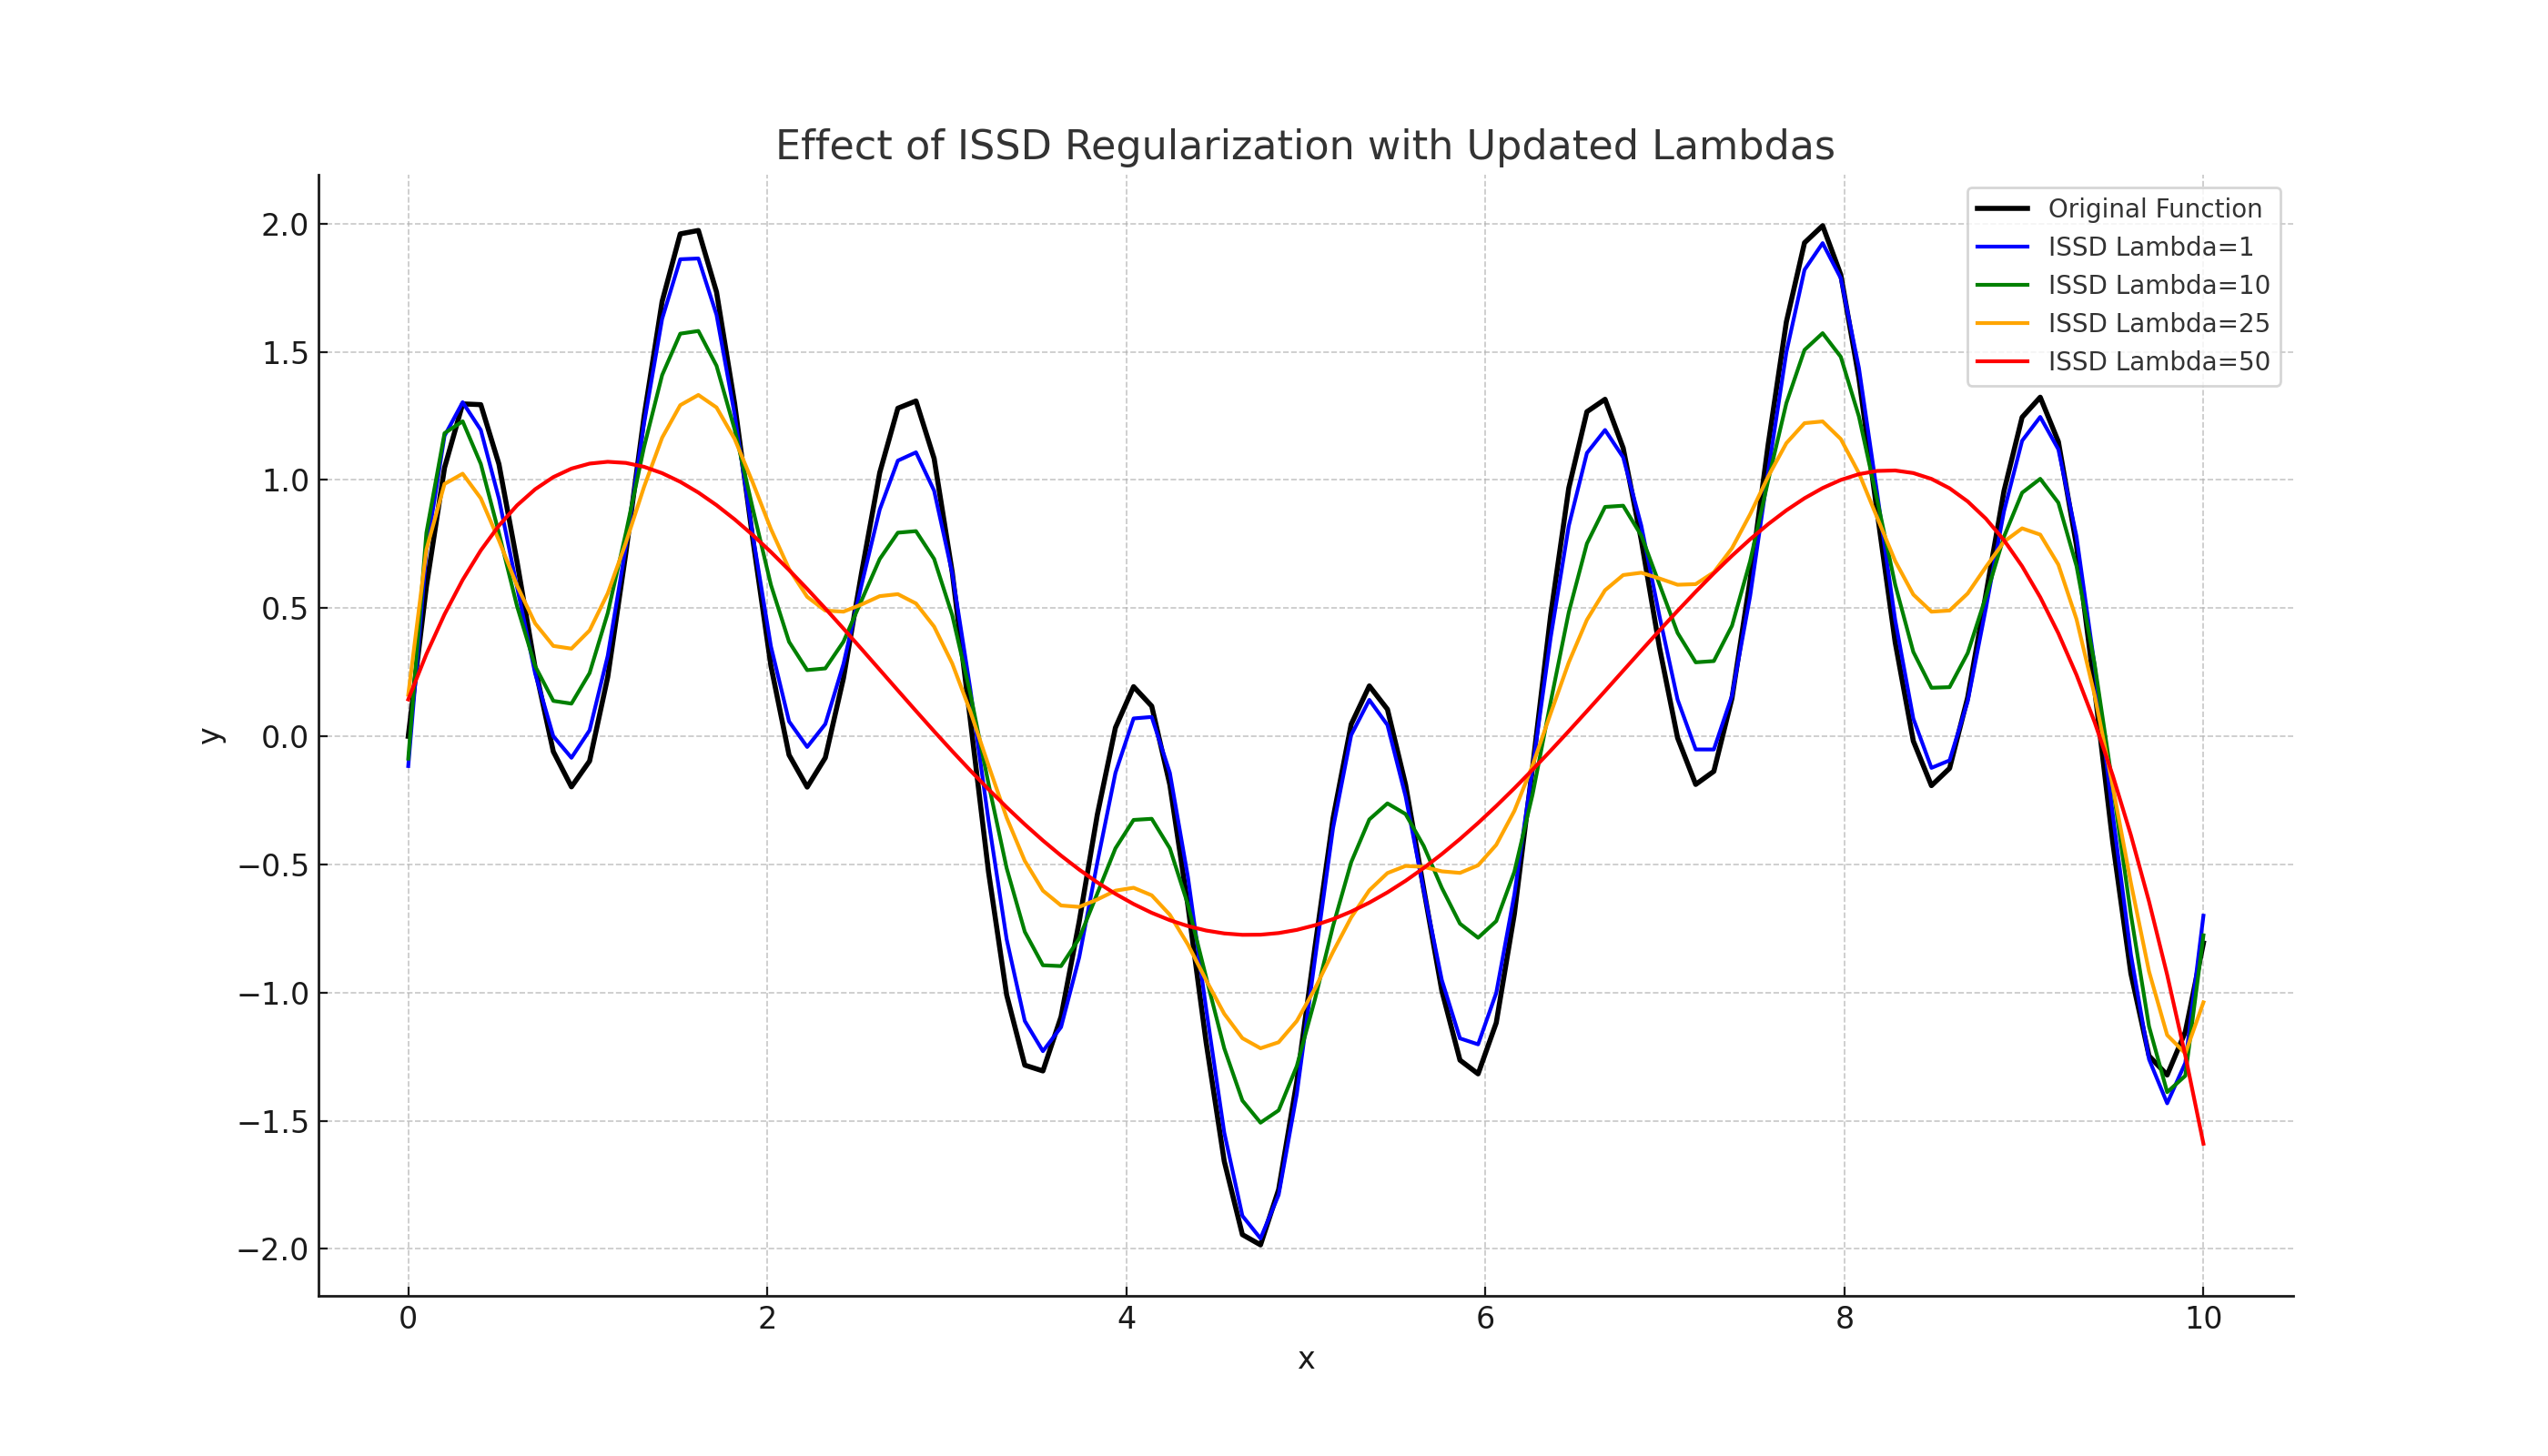
\includegraphics[width=0.9\textwidth]{visuals/Theory/issd_regularization_updated_lambdas.png}
\caption[Conceptual illustration of ISSD Regularization]{Conceptual illustration of ISSD Regularization: This figure shows the spline approximation of the function \(f(x) = \sin(x) + \sin(5x)\), a wiggly function, to be interpreted as a highly noisy dataset. The spline here is created using Python's 'scipy.interpolate.UnivariateSpline' with B-spline basis functions. The plot illustrates the effect of ISSD regularization on a spline model approximating this function. The ISSD penalty, expressed as \( \beta^T \mathbf{S} \beta \), penalizes the curvature, leading to smoother model fits as the lambda values increase (\(1\), \(10\), \(25\), and \(50\)). This visualization demonstrates how ISSD regularization in statistical modeling can effectively smooth out excessive fluctuations, hence avoiding overfitting by not adhering too closely to the 'noise' in the data, as represented by the oscillations in \(f\). The transition from less to more smoothing showcases the role of curvature penalization in achieving a balance between data representation and model simplicity.}
\label{fig:issd_effect_adjusted}
\end{figure}


\subsection{Ridge Penalty}\label{sec:smooth:ridge}

The Ridge penalty, often used in the context of linear regression, could also be applicable to the smoothing of functions. Mathematically, the Ridge penalty for a smooth function \( f \) is defined as:

\begin{equation}
    P_{\text{Ridge}}(f) = \lambda \int [f(x)]^2 \, dx.
    \label{eq:Ridge_penalty}
\end{equation}

The Ridge penalty aims to constrain the function \( f \) by penalizing its magnitude. This approach will make the function stay closer to zero, which will effectively control its variance. It can be thought of as applying a "shrinkage" effect to the function. By penalizing the square of the function, it discourages large values of \( f \), leading to a smoother and less flexible function.

\subsubsection{Relationship between Integral Expression and Matrix Formulation of Ridge Penalty}\label{sec:smooth:ridge:relation}

Similarly to the ISSD case, we have the theoretical integral representation and a computational matrix formulation.
\newline
In regression models, the function \( f(x) \) is typically represented as a linear combination of predictor variables \( x \) with coefficients \( \beta \):
\begin{equation}
    f(x) = \beta^T x.
\end{equation}
\newline
The Ridge penalty in regression analysis directly penalizes the squared coefficients, leading to the matrix form:
\begin{equation}
    \lambda \beta^T \mathbf{I} \beta,
\end{equation}
where \( \mathbf{I} \) is the identity matrix. This form effectively squares and sums each coefficient, mirroring the integral form's penalization of the function's magnitude.

\subsubsection*{Connection Between Forms}
The matrix form \( \lambda \beta^T \mathbf{I} \beta \) is a discrete approximation of the continuous integral form \( \lambda \int [f(x)]^2 \, dx \) when \( f(x) \) is represented in a regression context. The identity matrix \( \mathbf{I} \) ensures that each coefficient is squared and added, akin to integrating the square of the function over its domain.

\textbf{Note:} \( \lambda \beta^T \mathbf{I} \beta \) may be written equivalently as \( \lambda \|\beta\|^2 \).
\newline

\begin{figure}[H]
\centering
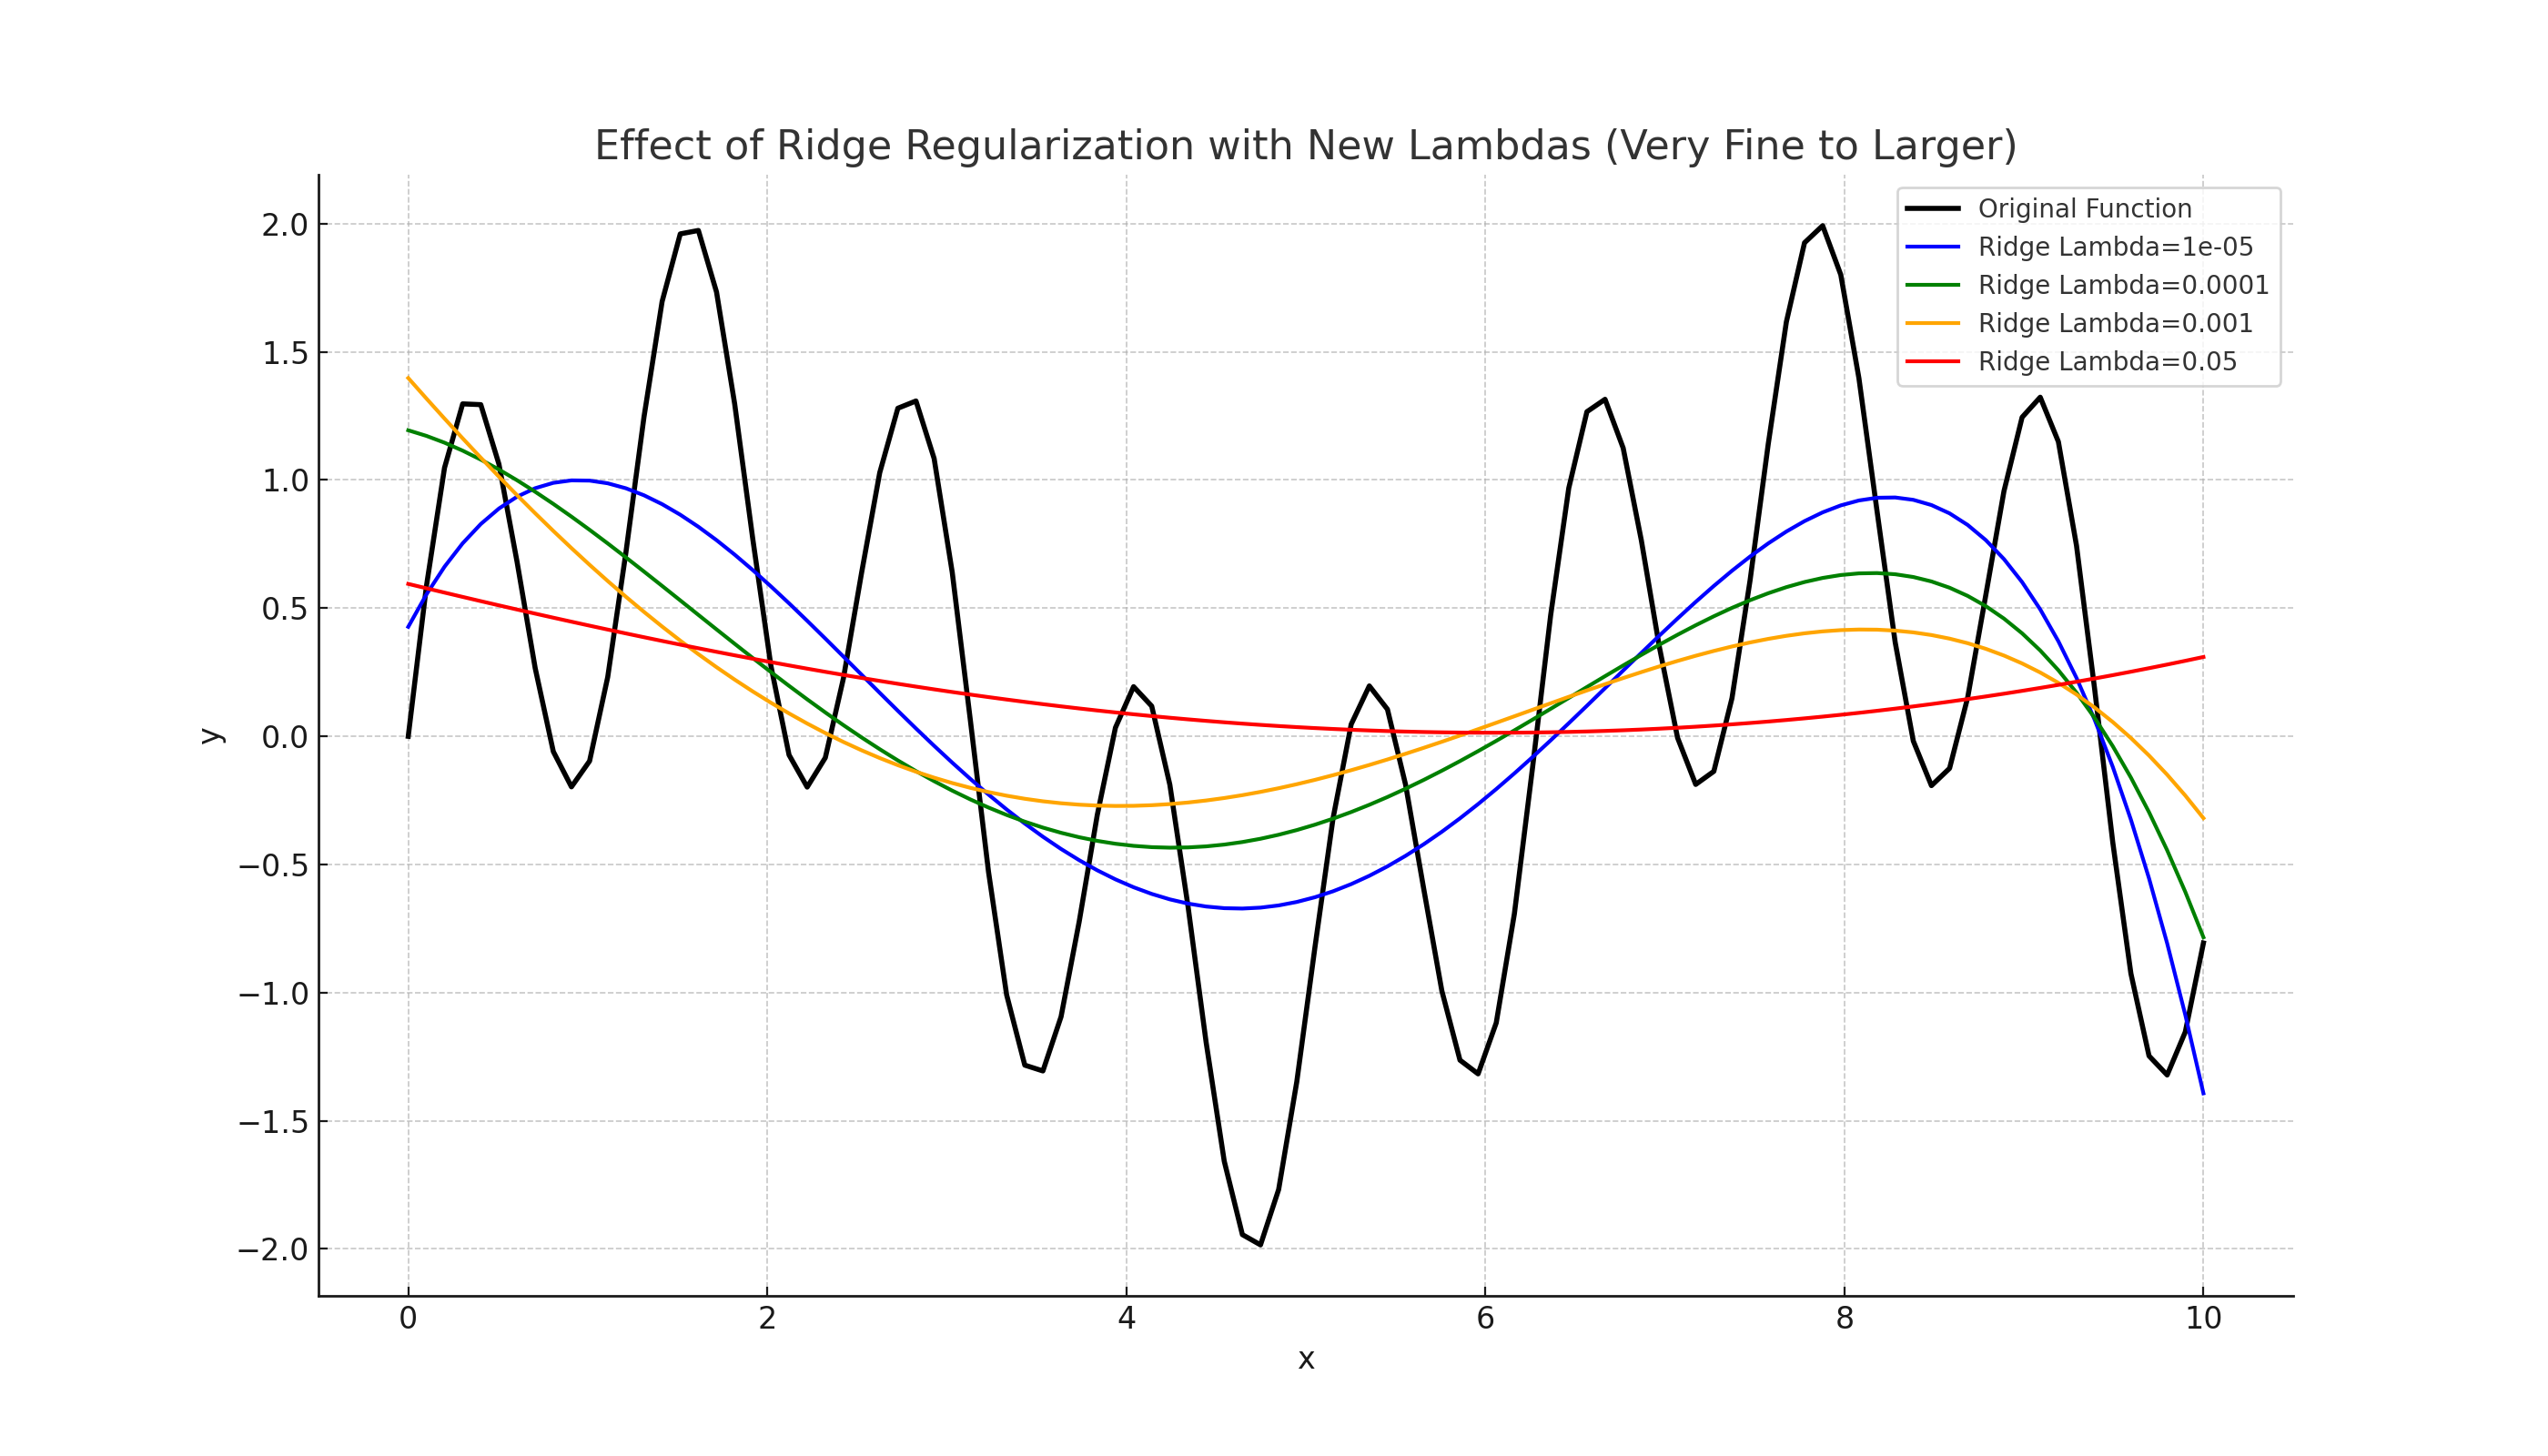
\includegraphics[width=0.9\textwidth]{visuals/Theory/ridge_regularization_new_lambdas.png}
\caption[Conceptual Illustration of Ridge Regularization]{Conceptual Illustration of Ridge Regularization: This figure shows the same spline approximation of the function \(f(x) = \sin(x) + \sin(5x)\), again interpreted as a highly noisy dataset. Here  Ridge penalties (\( \lambda \|\beta\|^2 \)) with increasing lambda values \(1e-5\), \(1e-4\), \(1e-3\), and \(5e-2\) are applied. We see a clear transition from wiggly to smoother fits which illustrates the Ridge regularization's effect: controlling complexity and avoiding overfitting by not capturing excessive 'noise' (analogous to the wiggles in \(f\)). We will come back to further analyze the efficacy of Ridge regularization in the final chapter of the paper.}
\end{figure}

\subsection{Strategies for Choosing Smoothing Parameter}\label{sec:smooth:lambda}

The selection of the appropriate value of the smoothing parameter \(\lambda\) in spline regression models is an important step to make sure an optimal balance between model complexity and data fitting is present. Different strategies can be employed to choose the optimal \(\lambda\), each with its specific mathematical framework and practical considerations. The primary goal is to minimize overfitting while retaining the model's predictive accuracy.

\subsubsection{K-Fold Cross-Validation}\label{sec:smooth:lambda:kfold}
K-Fold Cross-Validation is a resampling technique used to evaluate the model's performance. The dataset is divided into \(K\) equal-sized subsets. For each round of validation, \(K-1\) subsets are used to train the model, and the remaining subset is used as a test set to evaluate model performance. The process is repeated \(K\) times, with each subset used exactly once as the test set. The \(\lambda\) value is chosen based on the average error across all \(K\) tests. Mathematically, the optimal \(\lambda\) minimizes the Cross-Validation error, defined as:

\begin{equation}
    CV(\lambda) = \frac{1}{K} \sum_{k=1}^{K} MSE_k(\lambda),
    \label{eq:K_fold_CV}
\end{equation}

where \(MSE_k(\lambda)\) is the Mean Squared Error for the \(k\)-th fold. Intuitively, this method assesses the model's ability to generalize to unseen data, so that the chosen \(\lambda\) does not tailor the model excessively to the specificities of the training dataset.

\subsubsection{Generalized Cross-Validation}\label{sec:smooth:lambda:gcv}
Generalized Cross-Validation (GCV) is a computationally efficient approximation of Leave-One-Out Cross-Validation, particularly beneficial for large datasets. GCV estimates the model's predictive performance without the need to repeatedly re-fit the model for each datum. 

We can formulate GCV as follows:

\begin{equation}
    GCV(\lambda) = \frac{\sum_{i=1}^{n} (y_i - \hat{y}_i(\lambda))^2}{(1 - \frac{tr(\mathbf{A}(\lambda))}{n})^2},
    \label{GCV2}
\end{equation}

where \(y_i\) are the observed data points, \(\hat{y}_i(\lambda)\) are the predicted values under smoothing parameter \(\lambda\), \(n\) is the number of observations, and \(tr(A(\lambda))\) is the trace of the influence matrix \(A\) (for the chosen \(\lambda\)). This formulation is particularly relevant in spline regression, where the influence matrix plays a central role with respect to the GCV score \citet{wood2017} (p.171).
\newline

We can implement this in \texttt{glmmTMB} by considering the effective degrees of freedom, \(edf_{\lambda}\), for a given \(\lambda\).

\begin{equation}
    GCV(\lambda) = \frac{\sum_{i=1}^{n} (y_i - \hat{y}_i(\lambda))^2}{(1 - \frac{edf_{\lambda}}{n})^2},
    \label{GCV1}
\end{equation}

In both cases, the optimal \(\lambda\) is the one that minimizes \(GCV(\lambda)\). GCV adjusts the mean squared error by a penalty that increases with model complexity, thus favoring smoother, more generalizable models. The computational over efficiency over LOO-CV comes from computing the trace of the mean of \(\mathbf{A}_{ii}\) i.e $tr (\mathbf{A} / n )$ rather than for all $\mathbf{A}_{ii}$, \citep{wood2017}. 
\newline

\textbf{Note:} In binomial spline regression models, where the response variable is binary, Generalized Cross-Validation (GCV) requires special consideration. The binary nature of the response and the use of link functions necessitate a modified approach to calculating residuals and assessing model fit. GCV in this context relies on a deviance-based measure rather than the traditional sum of squared residuals.


\subsubsection{Maximum Likelihood (ML) and Restricted Maximum Likelihood (REML)}\label{sec:smooth:lambda:mlreml}
In addition to K-Fold Cross-Validation and GCV, Maximum Likelihood (ML) and Restricted Maximum Likelihood (REML) are robust methods for selecting the smoothing parameter.

Both ML and REML offer a more robust approach to smoothness selection compared to GCV with respect to overfitting. They inherently account for the model's complexity, making them particularly effective in scenarios where the response variable's relationship with predictors is complex and nonlinear.

\subsubsection{Limitations of Generalized Cross-Validation}\label{sec:smooth:lambda:limgcv}
While GCV is a widely used and computationally efficient method for selecting the smoothing parameter in spline models, it has certain limitations and is known to undersmooth in many cases, especially when paired with curvature-based regularization (\citet{wood2017}, p. 266).
\newline

\begin{itemize}
    \item \textbf{Sensitivity to Model Complexity:} GCV can be overly sensitive to the model's complexity. In models with high-dimensional data or complex underlying structures, GCV might underestimate the required smoothness, leading to undersmoothing.
    
    \item \textbf{Flat GCV Profiles:} For certain datasets, especially those with curvature-based penalties like in thin plate splines, the GCV criterion can have a flat profile. This flatness makes it difficult to discern the optimal value of \(\lambda\), as small changes in \(\lambda\) do not significantly affect the GCV score.
    
    \item \textbf{Random Variability and Overfitting:} The random variability in the data can lead GCV to favor models that are too flexible, capturing noise rather than the underlying trend. This is particularly problematic in curvature-based penalties, where the flexibility to fit local features can result in excessively wiggly fits.
\end{itemize}


\subsubsection{Alternative Approaches}\label{sec:smooth:lambda:alt}

The selection of an optimal smoothing parameter can also be effectively guided by the Corrected Akaike Information Criterion (AICc) and visual inspection of the model fit. AICc, an extension of the traditional AIC, is particularly suited for smaller sample sizes or models with a large number of parameters. It not only accounts for the goodness of fit but also includes a penalty for the number of parameters, thus discouraging overfitting. The correction in AICc can become important in spline models where the effective degrees of freedom can be substantial. When using AICc, the preferred model is the one with the lowest AICc value, balancing model complexity against the risk of overfitting. Complementing this quantitative measure, visual inspection of the fitted spline curves against the data provides an intuitive and direct assessment of the model’s adequacy. Domain knowledge of the distribution of the data and behaviour of the phenomena can inform how much or how many times you expect the predictive functional to bend. Examining residual plots and the smoothness of the fitted curves to ensure they capture the underlying data pattern without introducing artificial oscillations or ignoring significant trends is also an important step. Combining AICc with visual diagnostics offers a robust strategy for selecting the smoothing parameter, aligning statistical rigor with practical model interpretation and validation. 
\newline


\begin{figure}[H]
    \centering
    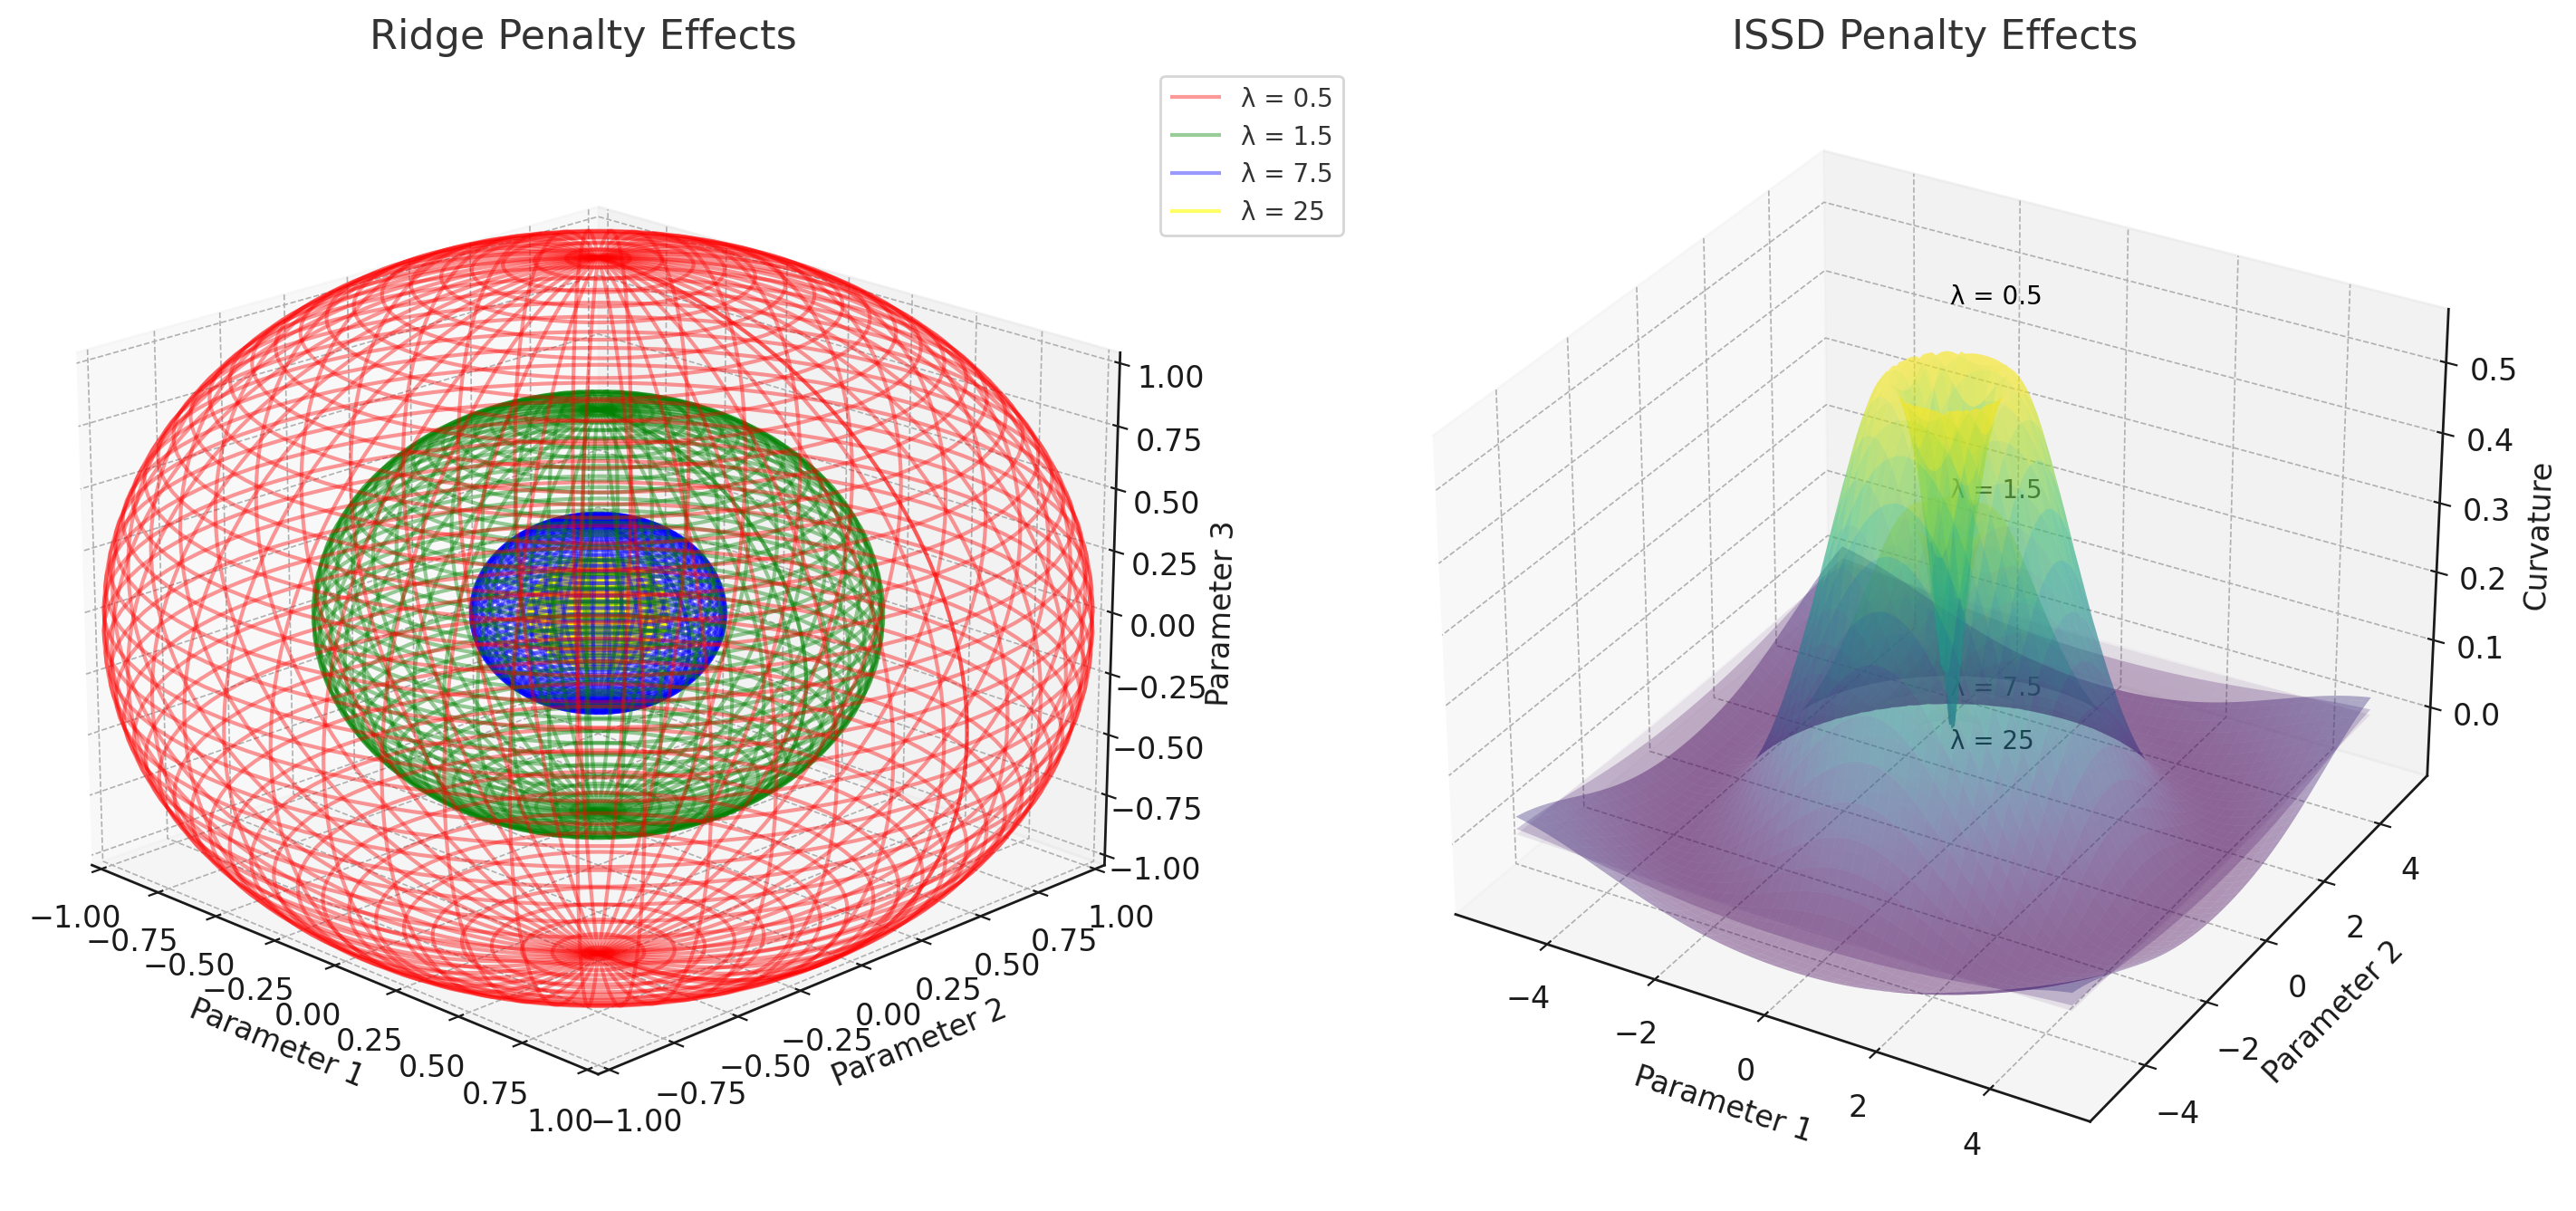
\includegraphics[width=\textwidth]{visuals/Theory/ridge_vs_issd_plot_nice.png}
    \caption{Conceptual Illustration of Ridge and ISSD Penalty Effects.}{Left: A conceptual visualization of a Ridge penalty effect on coefficients, shown as a series of ellipsoids in a three-dimensional parameter space. Each ellipsoid corresponds to a different regularization strength, demonstrating the constriction of the coefficient magnitudes as \(\lambda\) increases. Right: A two-dimensional parameter space with curvature (2nd order derivative) on the third axis to show the ISSD penalty's smoothing effect. The surfaces illustrate the reduction in curvature, with higher \(\lambda\) values leading to smoother, more flattened shapes. This figure aims to provide a visual representation of the differences in the two penalty approaches: Ridge directly penalizes coefficient magnitudes to limit overfitting, while ISSD gives model smoothness by penalizing curvature, rather than directly constraining parameter estimates. The visuals aren't direct comparisons, but show the influence of each penalty in a multidimensional parameter context.}
    \label{fig:ridge_vs_issd}
\end{figure}



\begin{table}[H]
\centering
\begin{tabular}{p{0.45\textwidth}p{0.45\textwidth}}
\hline
\textbf{Ridge Penalty Characteristics} & \textbf{ISSD Penalty Characteristics} \\
\hline
Preferred for data with multicollinearity & Suited for data with a naturally smooth underlying structure \\
Effective in high-dimensional settings where the number of predictors is high & Ideal for evenly distributed data without abrupt changes \\
Uniformly shrinks coefficients, addressing overfitting effectively & Smooths the function by penalizing high curvature, leading to a locally adaptive fit \\
Less sensitive to outliers, providing stable solutions & Can adapt to a specific level of smoothness, beneficial for data with consistent variability \\
Handles global structure in the data, making it suitable for complex models with multiple predictors & Preserves the interpretability of the model by maintaining the functional form \\
\hline
\end{tabular}
\caption{Comparison of data and model characteristics that are conducive to the use of Ridge versus ISSD penalties in regularization.}
\label{table:ridge_vs_issd}
\end{table}

\subsection{Overview of Forms of Smoothers}\label{sec:smooth:overview}

Generally we'll be dealing with three forms of smoothers: Isotropic, scale-invariant and tensor-product bases.

\subsubsection{Isotropic Smoothers}\label{sec:smooth:overview:isotropic}
Isotropic smoothers are uniform in all directions of the predictor space, ideal for spatial data or variables with similar scales.

\textbf{Characteristics:}
\begin{itemize}
    \item Uniform treatment of all input space directions.
    \item Optimal for data where directionality is irrelevant, such as circular or spherical data.
    \item Common in two-dimensional smoothing, like geographic data modeling.
\end{itemize}

\textbf{Example:} Thin Plate Regression Splines (TPRS) are examples of isotropic smoothers. These are often used in modeling geographic locations where latitude and longitude influence the response variable similarly.

\subsubsection{Scale Invariant Smoothers}\label{sec:smooth:overview:scale}
These smoothers adjust to the data scale, useful when predictors have different units or scales.

\textbf{Characteristics:}
\begin{itemize}
    \item Adapts to the scale of each predictor.
    \item Suitable for datasets with varied predictor scales or units.
    \item Common in models with mixed-type data, like financial datasets.
\end{itemize}

\textbf{Example:} Adaptive Splines, which can adjust the degree of smoothing based on the scale of predictors, are an implementation of scale invariant smoothers. They can be effective in economic data where variables like income and interest rates may have different scales.

\subsubsection{Tensor Product Smoothers}\label{sec:smooth:overview:tensor}
Designed for multidimensional smoothing, these smoothers combine univariate smoothers to allow predictor interactions.

\textbf{Characteristics:}
\begin{itemize}
    \item Facilitate modeling interactions between two or more predictors.
    \item Create multidimensional smoothing surfaces by combining lower-dimensional smoothers.
    \item Ideal for scenarios where interaction effects are important, such as in environmental models.
\end{itemize}

\textbf{Example:} Tensor Product Splines can be used in cases where interaction effects between predictors, like temperature and humidity, could reveal additional information in climate modeling.

\subsection{Quadratically Penalized Smoothers \&  Gaussian Random Fields}\label{sec:gaussian_random_quad_pen_smooth_equal}

Understanding the relationship between quadratically penalized smoothers and Gaussian random fields is key in leveraging the smooth construction machinery of \texttt{mgcv}, to random effects in glmmTMB. Recalling from sections \ref{sec:regmod:linmixmod:re} and \ref{sec:smooth:penreg:penreg} we can summarize the concepts:

\paragraph{Quadratically Penalized Smoothers}\label{sec:gaussian:quadpen}
Quadratically penalized smoothers minimize the residual sum of squares with an added quadratic penalty for excessive curve wiggles, i.e we minimize the expression:

\begin{equation}
    \text{minimize} \quad \left( \sum_{i=1}^{n} (y_i - f(x_i))^2 + \lambda \int [f''(x)]^2 dx \right).
    \label{eq:quadratic_penalty}
\end{equation}

\paragraph{Gaussian Random Effects}\label{sec:gaussian:re}
Gaussian random effects in mixed models address correlation or non-constant variance within data groups, assuming these effects follow a normal distribution;

\begin{equation}
\boldsymbol{y} = \mathbf{X}\boldsymbol{\beta} + \mathbf{Z}\boldsymbol{u} + \boldsymbol{\epsilon}, \quad \boldsymbol{u} \sim \mathcal{N}(0, \mathbf{G}).
\label{eq:gaussian_random_effects}
\end{equation}

\paragraph{Deriving an "Equivalence" of Smoothers and Random Effects}\label{sec:gaussian:equivalence}
The equivalence of these two, seemingly quite different and distinct concepts, lies in the interpretation of the quadratic penalty and Gaussian random effects. We want to show that

\begin{equation}
    \boldsymbol{u}^T \mathbf{G}^{-1} \boldsymbol{u} \quad \text{corresponds to} \quad \lambda \int [f''(x)]^2 dx .
    \label{eq:equivalence}
\end{equation}

In this relationship, the penalized smoother is viewed as a mixed model with basis coefficients \( u \) as random effects and the covariance matrix \( \mathbf{G} \) determined by the penalty term.
\newline

The derivation of the mathematical duality can be summarized in the following steps, as shown by \citet{wood2017}:

\begin{enumerate}
    \item Consider the LMM with Gaussian random effects in \ref{eq:gaussian_random_effects}
    with the likelihood function:
    \begin{equation}
    \mathcal{L}(\boldsymbol{\beta}, \boldsymbol{u} | \boldsymbol{y}) = f(\boldsymbol{y} | \mathbf{X}\boldsymbol{\beta} + \mathbf{Z}\boldsymbol{u}).
    \label{eq:lmm_likelihood}
    \end{equation}
    
    \item A GAM with a quadratic penalty is expressed as:
    \begin{equation}
    \hat{\boldsymbol{\beta}} = \arg\min_{\boldsymbol{\beta}} \left\{ -\log \mathcal{L}(\boldsymbol{\beta} | \boldsymbol{y}) + \lambda \boldsymbol{\beta}^T \mathbf{S} \boldsymbol{\beta} \right\},
    \label{eq:gam_penalty}
    \end{equation}
    where \( \mathbf{S} \) is the penalty matrix.
    
    \item The penalized log-likelihood for the GAM can be compared to the LMM log-likelihood:
    \begin{equation}
    -\frac{1}{2} (\boldsymbol{y} - \mathbf{X}\boldsymbol{\beta} - \mathbf{Z}\boldsymbol{u})^T (\boldsymbol{y} - \mathbf{X}\boldsymbol{\beta} - \mathbf{Z}\boldsymbol{u}) - \frac{1}{2} \boldsymbol{u}^T \mathbf{G}^{-1} \boldsymbol{u} \quad \text{and} \quad -\log \mathcal{L}(\boldsymbol{\beta} | \boldsymbol{y}) + \lambda \boldsymbol{\beta}^T \mathbf{S} \boldsymbol{\beta}.
    \label{eq:equivalence_derivation}
    \end{equation}

    By appropriate choices of \(\mathbf{G}\) and \(\mathbf{S}\), specifically setting \(\mathbf{G}^{-1} = \lambda \mathbf{S}\), we observe a correspondence between the random effects in a mixed model smoothers in a GAM. The precision matrix (\(\mathbf{G}^{-1}\)) of the random effects in a LMM is directly proportional to the penalty matrix (\(\mathbf{S}\)) in a GAM, adjusted by the smoothing parameter \(\lambda\).

We can summarize the correspondence we've derived as follows:
\begin{itemize}
    \item In LMMs, the random effects are regularized by their covariance matrix, \(\mathbf{G}\), which determines their spread and correlation structure. The inverse of this matrix, \(\mathbf{G}^{-1}\), is important in constraining these effects during model fitting.
    \item In GAMs, smooth terms are regularized by a penalty to avoid overfitting, with the strength and structure of this penalization defined by \(\lambda\) and the penalty matrix \(\mathbf{S}\).
\end{itemize}
\end{enumerate}

This result is the foundation for understanding the relationship between mixed modeling and smoothing methods. The mathematical similarity between the two models provides the potential for estimating smooths in mixed model frameworks, and vice versa.

\section{R packages 'mgcv' and 'glmmTMB'}\label{sec:rpack:}

\subsection{mgcv}\label{sec:rpack:mgcv}

The \texttt{mgcv} package, developed primarily by Simon Wood, is a highly optimized and powerful framework for fitting GAMs. It's  become the benchmark and standard framework in R for these models due to its flexibility, efficiency, and the range of functionalities it offers. Its extensive infrastructure and many utility functions for developers, makes it an obvious choice for smooth construction for use in \texttt{glmmTMB}. Some of it's key features include:

\begin{itemize}
    \item \textbf{Comprehensive GAM Support:} \texttt{mgcv} is optimized for fitting many forms of GAMs, including models with complex smoothing structures and interactions between predictors.
    
    \item \textbf{Robust Smoothing Parameter Selection:} The package automates the selection of smoothing parameters using methods like Generalized Cross-Validation (GCV).
    
    \item \textbf{Advanced Smoothing Techniques:} It supports many types of smoothers (via choices of basis functions), allowing for great flexibility while modeling.
    
    \item \textbf{Model Diagnostics and Visualization:} It includes many tools for model checking, plotting and diagnostics.
    
    \item \textbf{Extensions to GLMMs:} Importantly it also has utility (smooth2random) to extend its capabilities to GLMMs, making it capable of estimating random hierarchical or clustered data, and transforming smooths to random effect representation.
\end{itemize}

\subsubsection{Simple Example}\label{sec:rpack:mgcv:ex}

To help get an idea of how \texttt{mgcv} look and work, we'll present a simple example of one, and provide short explanations for what's going on.
\textbf{Note: the s()} functions calls the \texttt{smoothCon} function, which is a wrapper for \texttt{smooth.construct}. More detail can be found in the Appendix and in \href{https://cran.r-project.org/web/packages/mgcv/mgcv.pdf}{mgcv documentation}.

\begin{lstlisting}[language=R][language=R]
library(mgcv€
data(mtcars€
g1 <- gam(mpg ~ s(hp, k = 30, bs = "tp"€ + s(wt€, 
data = mtcars€
\end{lstlisting}

\begin{itemize}
  \item \texttt{hp}: The predictor variable.
  \item \texttt{k}: The maximum  degrees of freedom to use for representing the smooth term.
  \item \textbf{bs}: The type of basis to use for the smooth term. Common choices include "tp" for thin plate splines and "cr" for cubic regression splines.
\end{itemize}

\subsection{Smooth Construction in \texttt{mgcv}}\label{sec:rpack:smoothcon}

Smooth construction is the process in \texttt{mgcv} package which creates the actual smooth object (smoother), according to the basis function type and any other arguments specified. The internal function \texttt{mgcv::smooth.construct} handles the construction of the smooth. This function is usually called by the wrapper function \texttt{smoothCon()} which is interfaced on the surface level by the user with the \texttt{s()}, \texttt{te()} or \texttt{t2()} functions.

\textbf{The Role of \texttt{smooth.construct}:}
\begin{itemize}
    \item \textbf{Custom Smooth Creation:} This function builds smooth terms using specified basis functions and smoothing parameters, and is the central internal function for translating smooth specifications into usable smooth objects in GAMs.
    
    \item \textbf{Versatile Basis Functions:} It supports many different basis functions, such as cubic regression splines and thin plate splines, enabling diverse data modeling.
    
    \item \textbf{Smoothing Parameter Estimation:} \texttt{smooth.construct} automates the estimation of smoothing parameters, balancing model fit and smoothness to prevent overfitting.
\end{itemize}

\textbf{The \texttt{smoothCon}:}
\begin{itemize}
    \item \textbf{Simplification and Accessibility:} \texttt{smoothCon} is a wrapper function for \texttt{smooth.construct} which creates smooths in the \texttt{mgcv} framework. I offers an intuitive interface for users, and it handles technical details, making smooth specification more accessible.
    
    \item \textbf{Integration with GAM Fitting:} This wrapper ensures compatibility of smooth objects with \texttt{mgcv}'s model fitting functions, enhancing ease of use and applicability across various data types.
\end{itemize}

In our manually specified models which uses a Ridge penalty, we use the \texttt{smoothCon} function to generate our smooth objects. An example of how a smooth object is created and re-parameterized is shown below. More detailed code for the implementation is in the Appendix and on \href{https://github.com/AllInCade/MasterProject/tree/main}{Github}. 

\begin{lstlisting}[language=R]
    sm_tmpd <- mgcv::smoothCon(s(tmpd, bs = "cs"€,
    absorb.cons = TRUE, data = chicago€[[1]]
    re_tmpd <- mgcv::smooth2random(sm_tmpd, "", type = 2€
\end{lstlisting}

\begin{itemize}
    \item The \texttt{tmpd} variable is used to construct a smooth term using the \texttt{smoothCon} function.
    \item The resulting smooth object, \texttt{sm\_tmpd}, comes from the specification \texttt{s(tmpd, bs = "cs")}.
    \item Setting \texttt{absorb.cons = TRUE} means identifiability constraints are absorbed into the penalized basis function matrix of the smooth, requiring an adjustment of the basis functions.
    \item The \texttt{smooth2random} function is then used to re-parameterize this smooth object so that it can be represented as a random effect, making it suitable for estimation within a mixed modeling framework.
    \item The choice of the basis type argument (\texttt{bs = "..."}) determines the structure of the smooth object, which includes:
    \begin{itemize}
        \item A penalized matrix of basis function coefficients, represented as random effects.
        \item Unpenalized coefficients of the intercept and linear term components, represented and fitted as fixed effects,(the null space of the smooth object).
    \end{itemize}
\end{itemize}


\subsection{glmmTMB}\label{sec:rpack:glmmTMB}

The \texttt{glmmTMB} \citep{GlmmTMB2017} package in R specializes in fitting generalized linear mixed models (\textbf{GLMMs}). One of its main strengths is its ease of use combined with quite advanced capabilities for zero-inflation, hurdle models, and more. 'TMB' stands for Template Model Builder, which refers to its use of efficient maximum likelihood estimation techniques.

\textbf{Key Features of \texttt{glmmTMB}:}
\begin{itemize}
    \item \textbf{Diverse Distribution Support:} Handles a variety of distributions including Poisson, negative binomial, gaussian, and beta.
    \item \textbf{Zero-Inflation and Hurdle Models:} Provides functionalities for zero-inflated and hurdle models, particularly useful for count data with excess zeros.
    \item \textbf{Complex Random Effects:} Supports complicated random effects structures, including nested and crossed effects.
    \item \textbf{Dispersion Models:} Ability to include covariates as dispersion parameters.
    \item \textbf{Conditional Models:} Facilitates conditional modeling with spatial or temporal auto-correlation structures.
\end{itemize}

\subsubsection{Simple Example}\label{sec:rpack:glmmTMB:ex}

Below is a simple example of how a \texttt{glmmTMB} can look, with some short explanations of the different parts of the model.

\begin{lstlisting}[language=R]
library(glmmTMB€
data("Salamanders"€
fit <- glmmTMB(count ~ spp + (1|site€,
disp =~ site,
zi = ~1, 
family = nbinom1(link="log"€, data = Salamanders€
\end{lstlisting}

\begin{itemize}
    \item \textbf{Fixed Effect:} \texttt{spp} - A predictor variable included as a fixed effect.
    
    \item \textbf{Random Effect:} $(1|\texttt{site})$ - Includes a random effect (intercept) for each `site`. This accounts for random variation between different sites, capturing unobserved heterogeneity.
    
    \item \textbf{Zero-Inflation Formula:} \texttt{zi =~ 1} - Specifies a zero-inflation part of the model. This lets's us model a separate process generating excess zeros in the count data, which is not explained by the main model components.

    \item \textbf{Dispersion Formula:} \texttt{disp =~ site} - Specifies a separate dispersion model. Allows us to model additional dispersion (variance) as a function of the \texttt{site} variable..
    
    \item \textbf{Distribution of Response:} \texttt{family = nbinom1(link = "log")} - The response variable is modeled using a negative binomial distribution (with a log-link), common for count data which shows overdispersion.
\end{itemize}

\subsection{Template Model Builder}\label{sec:rpack:TMB}

\textbf{TMB} is a high-performance tool for fitting statistical models. It uses maximum likelihood estimation based on Laplace approximation. A key computational component of TMB is automatic differentiation, imported from \texttt{CppAD}. It is written in \texttt{C++} for computational efficiency and is interfaced with \textbf{R} through the \texttt{TMB} package. \textbf{TMB} is very efficient at computing and estimating random effects, and as a result is well-suited for complex hierarchical models, such as generalized linear mixed models.
\newline

TMB is designed to handle a wide variety of models in general, but in \texttt{glmmTMB} we will be working with GLMMs of the form described in \ref{sec:regmod:glmm}:

\begin{equation}
    \boldsymbol{y} = \mathbf{X}\boldsymbol{\beta} + \mathbf{Z} \boldsymbol{u} + \boldsymbol{\epsilon}, \quad \boldsymbol{u} \sim N(0,\mathbf{G}), \quad \boldsymbol{\epsilon} \sim N(0, \mathbf{R}),
\label{eq:glmmtmb}
\end{equation}

Here is an overview of some of the core features of TMB;

\begin{itemize}
    \item \textbf{Programming Language:} Written in \texttt{C++} for flexibility and performance.
    \item \textbf{Derivative Calculation:} Computes first and second-order derivatives of likelihood or any \texttt{C++} written function.
    \item \textbf{R Integration:} Objective functions callable from R, enabling parameter estimation.
    \item \textbf{Laplace Approximation:} Applies Laplace approximation to function arguments for marginal likelihood.
    \item \textbf{Standard Deviation via Delta Method:} Calculates standard deviations for parameters or derived parameters.
    \item \textbf{Data Processing:} Handles pre and post-processing of data in R.
    \item \textbf{Software Foundation:} Based on CppAD and Eigen (C++ libraries for Automatic Differentiation and matrix operations).
\end{itemize}

\subsection{Automatic Differentiation}\label{sec:rpack:AD}

Automatic Differentiation (AD) is a computational technique used for efficiently and accurately calculating derivatives of functions. Unlike numerical differentiation which approximates derivatives using finite differences, and symbolic differentiation which computes derivatives analytically, AD decomposes functions into a sequence of elementary operations and applies the chain rule to these operations.

\subsubsection{Principles of AD}\label{sec:rpack:AD:principles}
AD operates on the premise that any computational function, regardless of complexity, can be broken down into elementary operations such as addition, multiplication, and elementary functions like sin, exp, and log \citep{WikiAutomaticDiff2024}. These operations form the computational graph, where each node represents an elementary operation, and edges represent the flow of operands. AD then traverses this graph to compute derivatives.

\subsubsection{Modes of AD}\label{sec:rpack:AD:modes}
There are primarily two modes of AD, called forward accumulation and backward accumulation. The terms forward mode and reverse mode are perhaps more used in machine learning contexts.
\begin{itemize}
    \item \textbf{Forward Accumulation:} In this mode, derivatives are propagated alongside the computation from inputs to outputs. It is efficient for functions with few inputs and many outputs. An example of one such application is sensitivity analysis which aims to analyze how a small change in one input variable affects multiple output variables.
    \item \textbf{Reverse Accumulation:} Here, derivatives are propagated backward from outputs to inputs, which is computationally advantageous for functions with many inputs and few outputs. A special case of backward accumulation, called back-propagation, is widely used in machine learning for gradient descent optimization. Particularly, deep neural networks (like convolutional neural networks) heavily rely on back propagation to update the loss function w.r.t to the weights of the network. 
\end{itemize}

\subsubsection{Computational Efficiency}\label{sec:rpack:AD:efficiency}
The primary advantage of AD over other differentiation methods is its computational efficiency and accuracy. AD computes derivatives up to machine precision, avoiding the pitfalls of round-off errors and numerical instability that are common in numerical differentiation. Furthermore, the avoidance of symbolic manipulation, as seen in symbolic differentiation, makes AD more scalable and suitable for large-scale problems.


\subsection{Laplace Approximation in TMB for GLMMs}\label{sec:rpack:Laplace}
TMB allows for complex model fitting, and is proven highly effective in fitting GLMMs. The Laplace approximation in this context involves a nested optimization procedure comprising an inner and an outer problem.

\subsubsection{Inner Optimization Problem}\label{sec:rpack:Laplace:inner}
The inner problem involves optimizing the conditional distribution of the random effects given the fixed effects. Mathematically, this can be expressed as finding the mode (which is also the mean for Gaussians) of the random effects (\(\boldsymbol{u}\)) distribution, conditional on the current estimate of fixed effects (\(\boldsymbol{\beta}\)). This optimization can be represented as:

\begin{equation}
    \hat{\boldsymbol{u}} = \arg \max_{\boldsymbol{u}} \log p(\boldsymbol{u} | \boldsymbol{\beta}, \boldsymbol{y}, \mathbf{X}, \mathbf{Z}).
\end{equation}

Gradient-based methods, computed by AD, are often employed to efficiently find these conditional modes.

\subsubsection{Outer Optimization Problem}\label{sec:rpack:Laplace:outer}
The outer optimization problem is to maximize the marginal likelihood of the fixed effects. This is done by integrating out the random effects using the Laplace approximation. The marginal likelihood, after applying the Laplace method centered at \(\hat{\boldsymbol{u}}\), is approximated as:

\begin{equation}
    \log p(\boldsymbol{y} | \boldsymbol{\beta}, \mathbf{X}, \mathbf{Z}) \approx -\frac{1}{2} \log |\mathbf{G} + \mathbf{Z}^T\mathbf{R}^{-1}\mathbf{Z}| - \frac{1}{2} (\boldsymbol{y} - \mathbf{X}\boldsymbol{\beta} - \mathbf{Z}\hat{\boldsymbol{u}})^T \mathbf{R}^{-1} (\boldsymbol{y} - \mathbf{X}\boldsymbol{\beta} - \mathbf{Z}\hat{\boldsymbol{u}}).
\end{equation}

Optimization of the fixed effects (\(\boldsymbol{\beta}\)) is then performed via gradient-based methods, leveraging the derivatives of the marginal likelihood with respect to \(\boldsymbol{\beta}\), calculated using AD.

\subsubsection{Computational Considerations}\label{sec:rpack:Laplace:computational}
This nested structure of iterated optimizations can become computationally burdensome. Each evaluation of the marginal likelihood for a new set of fixed effects (\(\boldsymbol{\beta}\)) requires a re-optimization of the random effects (\(\boldsymbol{u}\)). This iterative process, especially in high-dimensional settings, consumes considerable computational resources, much due to repeated calculations of gradients and Hessians.

\textbf{Note:} The exact technical details of the Laplace Approximation scheme in TMB can be found in the source material \citet{Kristensen2016TMB}, as it goes beyond the scope of this project. 

\subsection{Model construction and estimation in glmmTMB}\label{sec:rpack:construct}

In \texttt{glmmTMB}, a generalized linear mixed model is constructed and estimated using the Template Model Builder (TMB) framework. An overview (omitting the technical details) of the fitting process is given below. A model is represented as:

\begin{equation}
g(E[Y]) = \mathbf{X} \boldsymbol{\beta} + \mathbf{Z}\boldsymbol{u} + \boldsymbol{\varepsilon},
\label{eq:linkglmm}
\end{equation}

where \( g \) is the link function, \( E[Y] \) is the expected value of the response variable \( Y \), \( \mathbf{X} \) and \( \mathbf{Z} \) are design matrices for fixed and random effects, respectively, \( \boldsymbol{\beta} \) and \( \boldsymbol{u} \) are vectors of fixed and random effect coefficients, and \( \boldsymbol{\varepsilon} \) is the error term.

\subsubsection{Fixed Effects Estimation}\label{sec:rpack:construct:fixed}

Fixed effects in \texttt{glmmTMB} are represented by the matrix \( \mathbf{X} \) and the coefficient vector \( \boldsymbol{\beta} \). The matrix \( \mathbf{X} \) is constructed from the observed data and includes an intercept and covariates. The Maximum Likelihood Estimation   procedure (in \texttt{TMB}) is used to estimate \( \boldsymbol{\beta} \), maximizing the likelihood function of the observed data given the model.

\paragraph{Design Matrix for Fixed Effects}

\begin{equation}
\mathbf{X} = \begin{pmatrix}
1 & x_{11} & x_{12} & \cdots & x_{1p} \\
1 & x_{21} & x_{22} & \cdots & x_{2p} \\
\vdots & \vdots & \vdots & \ddots & \vdots \\
1 & x_{n1} & x_{n2} & \cdots & x_{np}
\end{pmatrix}
\end{equation}

\subsubsection{Random Effects Estimation}\label{sec:rpack:construct:random}

Random effects are accounted for by the matrix \( \mathbf{Z} \) and the random effects vector \( \boldsymbol{u} \). The random effects are estimated by \texttt{TMB} using a combination of MLE and the Laplace approximation. As described earlier,the Laplace approximation simplifies the integral in the likelihood computation, which is especially important for models with complex random effect structures.

\paragraph{Design Matrix for Random Effects}

\begin{equation}
\mathbf{Z} = \begin{pmatrix}
z_{11} & z_{12} & \cdots & z_{1q} \\
z_{21} & z_{22} & \cdots & z_{2q} \\
\vdots & \vdots & \ddots & \vdots \\
z_{n1} & z_{n2} & \cdots & z_{nq}
\end{pmatrix}
\end{equation}

\subsubsection{Covariance Matrix Estimation}\label{sec:rpack:construct:covmat}

The covariance matrix \( \mathbf{G} \) for the random effects is also estimated using MLE, as part of the overall model fitting process. This matrix describes the variances and covariances of the random effects, capturing their underlying structure.

\paragraph{Covariance Matrix}

\begin{equation}
\mathbf{G} = \begin{pmatrix}
\sigma_{11} & \sigma_{12} & \cdots & \sigma_{1q} \\
\sigma_{21} & \sigma_{22} & \cdots & \sigma_{2q} \\
\vdots & \vdots & \ddots & \vdots \\
\sigma_{q1} & \sigma_{q2} & \cdots & \sigma_{qq}
\end{pmatrix}
\end{equation}

The estimation of the model in \texttt{glmmTMB} using \texttt{TMB}s MLE and Laplace approximation techniques ensures efficient and robust fitting, especially for complex models with multiple fixed and random effects.

\section{Implementing Smooth Terms in glmmTMB with \texttt{mgcv} machinery}\label{sec:makingsmooth}

The mathematical similarity between quadratically penalized smoothers in GAMs and Gaussian random effects in mixed models allows for the estimation of smooth terms as "type 2 random effects". This is leveraged in statistical modelling software to provide flexible and efficient ways to fit generalized additive models using mixed model frameworks. The process of implementing this in \texttt{glmmTMB} is detailed below, and relies heavily on the work of \citet{wood2017} and \texttt{mgcv}. The technical implementation in the code base is work in progress, primarily done by Ben Bolker.

\subsection{Smooth Construction using smoothCon}\label{sec:makingsmooth:smoothcon}

\begin{figure}[H]
\centering
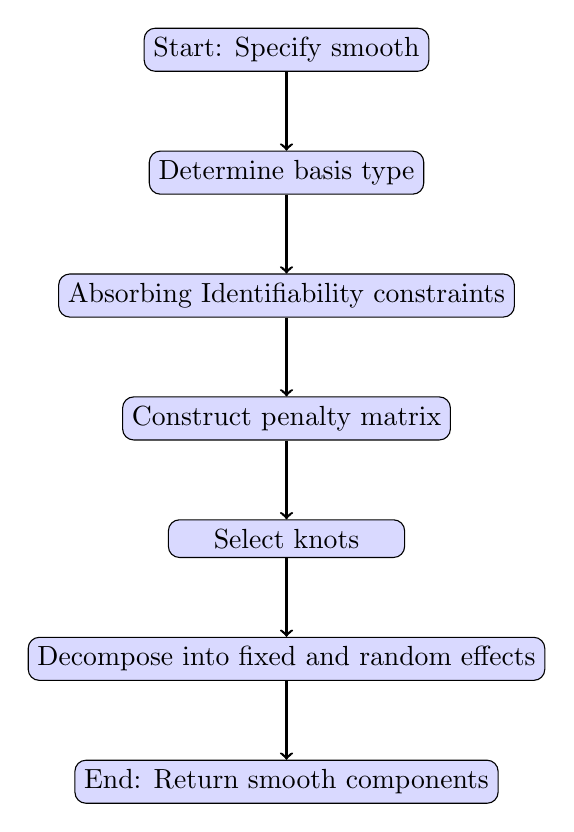
\begin{tikzpicture}[
    node distance=1cm,
    start chain=going below,
    every join/.style={->},
    every node/.style={draw, rounded corners, fill=blue!15, align=center, minimum width=3cm},
    arrow/.style={thick, ->}
]

% Nodes
\node (start) [on chain, join] {Start: Specify smooth};
\node (basis) [on chain, join] {Determine basis type};
\node (Absorb) [on chain, join] {Absorbing Identifiability constraints};
\node (penalty) [on chain, join] {Construct penalty matrix};
\node (knots) [on chain, join] {Select knots};
\node (decompose) [on chain, join] {Decompose into fixed and random effects};
\node (end) [on chain, join] {End: Return smooth components};

% Arrows
\draw [arrow] (start) -- (basis);
\draw [arrow] (basis) -- (Absorb);
\draw [arrow] (Absorb) -- (penalty);
\draw [arrow] (penalty) -- (knots);
\draw [arrow] (knots) -- (decompose);
\draw [arrow] (decompose) -- (end);

\end{tikzpicture}
\caption{Schematic overview of the \texttt{smoothCon} function from \texttt{mgcv}.}
\end{figure}


The \texttt{smoothCon} function in \texttt{mgcv} is a core utility designed to process smooth specifications in generalized additive models (GAMs). It essentially sets up the necessary matrices and information for representing and estimating the smooth components in the model. Here's an overview of its operation:

\begin{enumerate}[label=\arabic*., left=0pt]
    \item \textbf{Input Specification}: The function takes in a smooth specification, which consists of a combination of a predictor variable, a basis type (\texttt{bs} argument), and other options like the number of knots (\texttt{k} argument).
    
    \item \textbf{Determine Basis Type}: Based on the \texttt{bs} argument, \texttt{smoothCon} determines the type of basis functions to use. This choice influences the flexibility and shape of the smooth term. Common basis types include cubic splines (\texttt{cr}), thin plate splines (\texttt{tp}), and P-splines (\texttt{ps}), among others.

    \item \textbf{Absorbing Identifiability constraints}: \texttt{absorbs.cons=TRUE} ensures that the smooth terms are uniquely distinguishable and not confounded with other model components, like the intercept. The process employs QR decomposition, a mathematical method for transforming the basis functions such that they become orthogonal to the space of the constraints (e.g., the intercept). This orthogonality is essential because it prevents the overlap of effects between the smooth terms and the intercept, ensuring that each component of the model contributes distinctly to the explanation of the data. 

    
    \item \textbf{Construct Penalty Matrix}: One of the fundamental aspects of GAMs is the application of a penalty to the smooth terms to avoid overfitting. \texttt{smoothCon} constructs a penalty matrix appropriate for the chosen basis type. The penalty targets the "wiggly" (curvature) parts of the smooth to ensure a balance between fit and smoothness.
    
    \item \textbf{Select Knots}: Knots are specific points in the data range where the spline functions can change direction. \texttt{smoothCon} selects appropriate knot locations based on the data and the specified number of knots (\texttt{k} argument).
    
    \item \textbf{Decompose into Fixed and Random Effects}: For certain applications, especially when using GAMs in mixed model frameworks, the smooth terms can be decomposed into fixed and random effects components. \texttt{smoothCon} provides the necessary decomposition, allowing the smooth to be used in packages like \texttt{gamm4}.
    
    \item \textbf{Output}: The function returns a list containing various components representing the smooth, including the basis functions, penalty matrices, and other relevant information.
\end{enumerate}


\subsection{Re-parameterizing Using smooth2random}\label{sec:makingsmooth:smooth2random}

\paragraph{Duality of Gaussian Random Effects and Penalized Smooths}\label{sec:smooths:re:parametrization}

Recall the equivalence we derived between Gaussian random effects and penalized smooths in section \ref{sec:gaussian:equivalence}. Random effects in mixed models can be conceptualized and estimated as smooths, leveraging the flexibility of smooth modeling to capture complex random effects structures. Conversely, smooth terms in GAMs can be treated as random effects within a mixed model framework. In practical implementation this duality hinges on appropriate (re-)parameterization, allowing smooth terms to be integrated as random effects and vice versa. The transformation involves adjustments in the model matrix and the penalty structure, enabling the seamless transition between these two interpretations and estimation approaches.

\subsubsection{Natural Parameterization in GAMs}\label{sec:makingsmooth:smooth2random:natparams}

In the context of GAMs, the natural parameterization for smooth terms involves several key mathematical transformations. Given a model matrix \( \mathbf{X} \) and a penalty matrix \( \mathbf{S} \), the process is as follows:

\begin{itemize}
  \item Perform QR decomposition of \( \mathbf{X} \), yielding \( \mathbf{X} = \mathbf{QR} \).
  \item Reparameterize the penalty matrix \( \mathbf{S} \) as \( \mathbf{R}^{-T}\mathbf{SR}^{-1} \).
  \item Eigen-decompose this reparameterized penalty matrix to obtain \( \mathbf{R}^{-T}\mathbf{SR}^{-1} = \mathbf{UDU}^T \), where \( \mathbf{U} \) is an orthogonal matrix of eigenvectors, and \( \mathbf{D} \) is a diagonal matrix of corresponding eigenvalues.
  \item This leads to a new parameter vector \( \boldsymbol{\beta'} = \mathbf{U}^T\boldsymbol{\beta''} \), a transformed model matrix \( \mathbf{QU} \), and a modified penalty matrix \( \mathbf{D} \).
  \item The penalized parameter estimates are effectively shrunken versions of the unpenalized coefficients. The shrinkage factor is influenced by eigenvalues and the smoothing parameter \( \lambda \), reflecting the effective degrees of freedom of the model.
\end{itemize}


\subsubsection{Re-Parameterized Formulation for Mixed Models}\label{sec:makingsmooth:smooth2random:reparams}

For mixed model frameworks, smooth terms from Generalized Additive Models (GAMs) can be re-formulated to facilitate their integration. This re-parameterization is particularly useful when estimating smooths using software designed for generalized linear mixed models.
\newline

Consider \(\boldsymbol{f}\) as the vector of the smooth evaluated at observed covariate values. The smooth can be expressed in a mixed model form as
\[ \boldsymbol{f} = \mathbf{X}' \boldsymbol{\beta}' + \mathbf{Z}\boldsymbol{b}, \]
where \(\boldsymbol{b} \sim \mathcal{N}(0, \mathbf{I}\sigma^2_b)\). Then:
\begin{itemize}
  \item The columns of \(\mathbf{X}'\) form a basis for the null space of the smoothing penalty.
  \item The columns of \(\mathbf{Z}\) form a basis for its range space.
\end{itemize}

To construct \(\mathbf{X}'\) and \(\mathbf{Z}\), we partition matrix \(\mathbf{U}\) from eigen-decomposition of the smoothing penalty matrix into \(\mathbf{U} = [\mathbf{U}^+ : \mathbf{U}^0]\), where \(\mathbf{U}^+\) corresponds to eigenvectors with positive eigenvalues, and \(\mathbf{U}^0\) are the remaining eigenvectors. Thus
\[ \mathbf{X}' = \mathbf{QU}^0 \]
\[ \mathbf{Z} = \mathbf{QU}^+\mathbf{D}^{-1/2}. \]
This framework allows the smooth to be viewed and handled as a Gaussian random field within the mixed model structure.


\subsubsection{Re-Parameterization by smooth2random}\label{sec:makingsmooth:smooth2random:reparamssmooth2random}

The re-parameterization described above is implemented in \texttt{mgcv} with the utility function \texttt{smooth2random}. It transforms smooth terms in their natural parameterization, designed for Generalized Additive Models (GAMs), to the re-parameterized form that is compatible with mixed model frameworks. 

\begin{itemize}
  \item \textbf{Eigen-Decomposition}: The function starts with an eigen-decomposition of the smooth's penalty matrix, obtaining the eigenvalues and eigenvectors. This corresponds to the process of deriving \( \mathbf{U} \) and \( \mathbf{D} \) in the natural parameterization.
  
  \item \textbf{Transformation Matrices Creation}: Utilizing these eigenvectors and eigenvalues, it constructs transformation matrices, changing from the natural parameterization.

  \item \textbf{Model Matrix Adjustment}: The original model matrix \( X \) is then transformed, effectively separating the penalized and unpenalized components, corresponding to the theoretical formulation of \( \mathbf{X}' \) and \( \mathbf{Z} \) in the mixed model representation, which again correspond to the \texttt{Xr} (penalized) and \texttt{Xf} (unpenalized/null space) matrices, respectively.

  \item \textbf{Random Effect Form}: The re-parameterized smooths are then estimated as random effects (with a dummy grouping variable) in the mixed model.
\end{itemize}

The smooth objects pass through \texttt{smooth2random} introduces some differences in estimates when compared to the natural GAM parameterization, due to the resulting basis function coefficient matrix being slightly altered.


\begin{figure}[H]
\centering
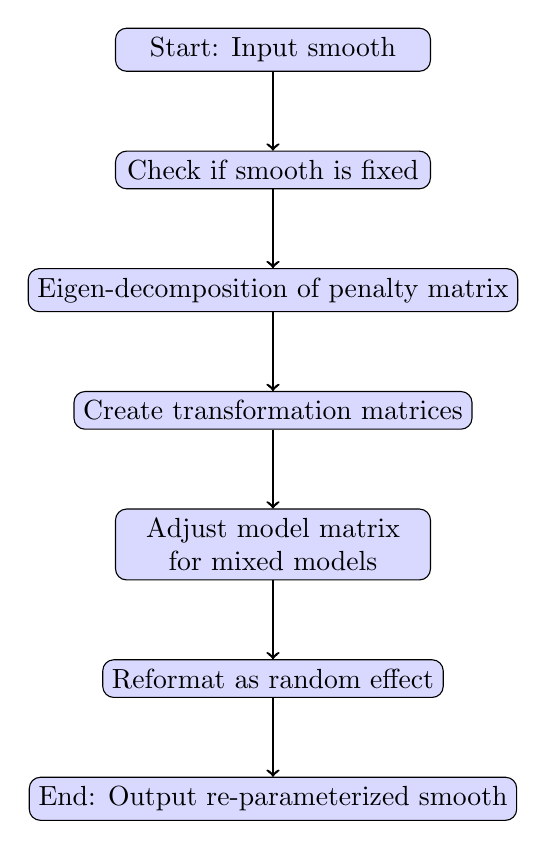
\begin{tikzpicture}[
    node distance=1cm, 
    start chain=going below,
    every join/.style={->},
    every node/.style={draw, rounded corners, fill=blue!15, align=center, minimum width=4cm},
    arrow/.style={thick, ->}
]

% Nodes
\node (start) [on chain] {Start: Input smooth};
\node (check) [on chain, join] {Check if smooth is fixed};
\node (eigen) [on chain, join] {Eigen-decomposition of penalty matrix};
\node (transform) [on chain, join] {Create transformation matrices};
\node (adjust) [on chain, join] {Adjust model matrix \\ for mixed models};
\node (reformat) [on chain, join] {Reformat as random effect};
\node (end) [on chain, join] {End: Output re-parameterized smooth};

% Arrows
\draw [arrow] (start) -- (check);
\draw [arrow] (check) -- (eigen);
\draw [arrow] (eigen) -- (transform);
\draw [arrow] (transform) -- (adjust);
\draw [arrow] (adjust) -- (reformat);
\draw [arrow] (reformat) -- (end);

\end{tikzpicture}
\caption{Schematic overview of the \texttt{smooth2random} function from \texttt{mgcv}.}
\end{figure}


\newpage


\subsection{How s() can be presented in \textbf{glmmTMB}}\label{sec:makingsmooth:s()}

While using the two functions \texttt{mgcv} functions discussed above, we can make the smoothing term in a \textbf{glmmTMB}-model.


\subsection*{R Code}

\begin{lstlisting}[language=R]
sm_tmpd <- mgcv::smoothCon(s(tmpd€, absorb.cons = TRUE, 
                           data = chicago€[[1]]             
re_tmpd <- mgcv::smooth2random(sm_tmpd, "", type = 2€
Xf_tmpd <- re_tmpd$Xf
Xr_tmpd <- re_tmpd$rand[[1]]
chicago$ID <- factor(rep(1, nrow(chicago€€€
ftmb1 <- glmmTMB(formula = death ~ Xf_tmpd +
                 homdiag(0 +Xr_tmpd | ID€, 
                 data = chicago, REML=TRUE€
\end{lstlisting}

\subsection*{Code Description}

\begin{enumerate}
    \item \textbf{Identifiability Constraints and Basis Function:}
    The code initializes a smooth term (\texttt{sm\_tmpd}) using \texttt{mgcv::smoothCon} with identifiability constraints absorbed into the basis, applicable to the variable \texttt{tmpd} in the \texttt{chicago} dataset.

    \item \textbf{Conversion to Random Effects:}
    The smooth term is then converted into random effects (\texttt{re\_tmpd}) using \texttt{mgcv::smooth2random}, specifying the type of conversion.

    \item \textbf{Extraction of Matrices:}
    Fixed effects matrix (\texttt{Xf\_tmpd}) and random effects matrix (\texttt{Xr\_tmpd}) are extracted from the converted smooth term.

    \item \textbf{Creating a Grouping Variable:}
    A fake grouping variable (\texttt{ID}) is created in the \texttt{chicago} dataset, assigning the same value to all observations for modeling purposes.

    \item \textbf{Generalized Linear Mixed Model (GLMM):}
    A GLMM (\texttt{ftmb1}) is fitted using \texttt{glmmTMB} to predict \texttt{death}, based on fixed effects and a random effect structure with a homogenous diagonal covariance structure, using Restricted Maximum Likelihood for estimation.
\end{enumerate}

\textbf{Note:} Type 1 Random Effects are akin to random intercepts in mixed models, where each group level has its own intercept, modeled using \texttt{s()} with \texttt{bs = "re"}. Type 2 Random Effects handle more complex variations like smooth random effects or random slopes, where each group level gets its own smooth function, implemented using \texttt{s()} with a grouping factor, as in \texttt{s(x, bs="fs", m=1, by=factor)}.



\subsection{Basis functions in \textbf{glmmTMB}}\label{sec:makingsmooth:bs}



\begin{table}[H]
\centering
\caption{Compatibility of Spline Types in \texttt{glmmTMB}}
\begin{tabular}{lccc}
\toprule
Spline & bs & Compatible & Reasoning \\
\midrule
Cubic Regression & \texttt{"cr"} & \checkmark &  \\
Cyclical Cubic & \texttt{"cc"} & $\times$ & Only one Xf-term \\
Cubic Smoothing & \texttt{"cs"} & $\times$ &  No Xf-terms \\
Thin Plate Regression & \texttt{"tp"} & \checkmark &   \\
B-splines & \texttt{"bs"} &  \checkmark &  \\
P-splines & \texttt{"ps"} &  \checkmark &  \\
Two-dimensional Tensor Product & \texttt{"t2"} & $\times$ & \\
Two-dimensional Tensor Product & \texttt{"te"} & $\times$ & Not supported by smooth2random (gamm4) \\
Shrinkage Smooth & \texttt{"fs"}  & \checkmark & \\
Adaptive & \texttt{"ad"}  &$\times$ & Not supported by smooth2random  \\
Random Effect & \texttt{"re"}  & $\times$ & No Xf-terms \\
% Add other splines as needed
\bottomrule
\end{tabular}
\end{table}


\subsubsection{Proposition for\texttt{ bs="cs"} and \texttt{bs="cc"}}\label{sec:makingsmooth:bs:prop}

The cyclical cubic regression spline and cubic smoothing spline do not have these \texttt{Xf} terms, fixed effects, and the model will therefore not work with the code given is section \ref{sec:makingsmooth:s()}. A seemingly nice alternative would be to code the model without the \texttt{Xf} terms, as all the information from these basis functions are given in the \texttt{Xr} terms:

\begin{lstlisting}[language=R]
    ftmb1 <- glmmTMB(formula = death ~ 
    homdiag(0+Xr_tmpd | fake_group€
    , data = chicago, REML=TRUE€
\end{lstlisting}

Later in the thesis we will do some comparison between this formula and a corresponding \textbf{GAMM} model with basis functions of cyclical and cubic smoothing splines to prove that it may be a solution.



\subsection{Complexities of Tensor Product Splines}\label{sec:makingsmooth:tensor}

Smooths of tensor product splines are more complicated and challenging to implement, due to their more complex construction and structure. One obstacle is handling the splitting of the model matrix into 4 matrices, three of which are \texttt{Xr}-matrices and one \texttt{Xf}-matrix. There is comprehensive mathematical theory on which construction methods for tensor product smooths are built (see \citet{wood2017}). Understanding the finer details and mechanisms of how tensor product splines are constructed by the smooth constructor is necessary for managing their implementation in \texttt{glmmTMB}. 

\subsubsection{Tensor Product Construction of Smooths in GAMs}\label{sec:makingsmooth:tensor:construction}

Fabian Scheipl's alternative tensor product construction in \texttt{mgcv} facilitates smooth term estimation using a method which simplifies mixed modeling by using non-overlapping penalty terms \citet{wood2017}. This construction yields a model with easily interpretable, rescaling-invariant smooth terms suitable for mixed effect modeling.

We begin with a set of unconstrained marginal smooths. The next step involves re-parameterizing each marginal so that the penalty matrix becomes an identity matrix, with \( M \) leading diagonal entries zeroed (\( M \) being the dimension of the penalty null space. This step includes a linear rescaling of parameters to equate the positive elements of the penalty matrix to 1.
\newline

We then divide each re-parameterized model matrix into columns \( \mathbf{X} \) and \( \mathbf{Z} \). \( \mathbf{X} \) corresponds to the zero elements on the leading diagonal of the penalty, and \( \mathbf{Z} \) to the unit entries, leading to \( \boldsymbol{f} = \mathbf{X} \boldsymbol{\delta} + \mathbf{Z}\boldsymbol{b} \). To enhance interpretability, it's preferable to have the constant function explicitly present in each marginal basis. An automatic re-parameterization method ensures this in the general case. For some function \( g \) in the penalty null space, the additional penalty \( P_N = \sum_i (g(x_i) - \bar{g})^2 \) shrinks \( g \) towards a constant function, i.e \( P_N = \boldsymbol{\delta}^T \mathbf{D}^T \mathbf{D} \boldsymbol{\delta} \), where \( \mathbf{D} = \mathbf{X}^{-1}_{1^T} \mathbf{X}/n \) and decomposed \( \mathbf{D}^T \mathbf{D} = \mathbf{U} \mathbf{\Omega} \mathbf{U}^T \).
\newline

Reparameterizing such that the null space model matrix is now \( XU \) ensures that the final column of the new model matrix is constant, assuming the original penalty's null space includes the constant function in its span.

For the \( d \) marginal smooths, the \( j \)th marginal has unpenalized model matrix \( X_j \) and penalized model matrix \( Z_j \) (with penalty \( I \)). We initialize matrices \( \gamma = \{X_1, Z_1\} \), or \( \gamma = \{[X_1], Z_1\} \) where \( [X_j] \) denotes the set of columns of \( X_j \), each treated as a separate matrix. The following steps are repeated for \( i \) from 2 to \( d \):

\begin{enumerate}
    \item Form row-wise Kronecker products of \( X_i \) (or of all columns \( [X_i] \)) with all elements of \( \gamma \).
    \item Form row-wise Kronecker products of \( Z_i \) with all elements of \( \gamma \).
    \item Append the matrices from the previous steps to the set \( \gamma \).
\end{enumerate}

The model matrix, \( X \), for the tensor product smooth is formed by appending all elements of \( \gamma \) columnwise. Each element of \( \gamma \) has an associated identity penalty with a smoothing parameter, except for elements involving no \( Z_j \) term, which are unpenalized. The variant using \( [X_j] \) instead of \( X_j \) ensures strict invariance with respect to linear rescaling of the covariates but requires extra penalty terms. 
\newline
Figure \ref{fig:tps} shows a smooth function \(f(z)\) is represented with a spline using six equidistant knots, with parameters varying smoothly along the \(x\)-axis. Each function parameter of \(f(z)\) is then modeled as a spline of \(x\). Scale invariance is ensured since separate smoothness penalties are applied in both the \(z\) and \(x\) directions. An \(x\)-direction penalty is formulated by summing \(\int \left[ f''(x) \right]^2 dx\) along the defined thin black curves. Similarly for a z-direction penalty.   \citet{wood2020}.

\begin{figure}[H]
    \centering
    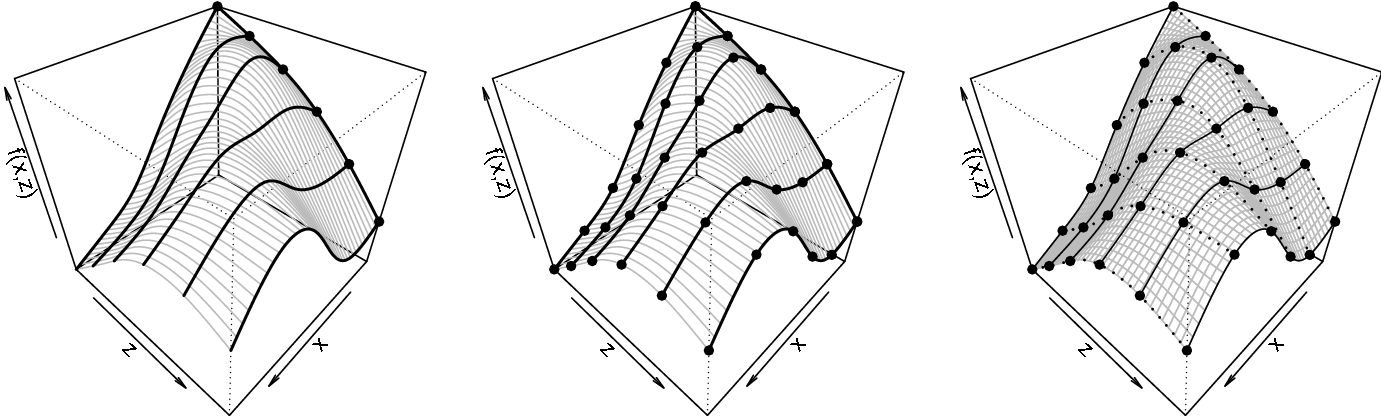
\includegraphics[width=0.9\textwidth]{visuals/Theory/tensor_product_smooth.png}
    \caption{Tensor product smooth construction illustrated through a symmetric process in x and z dimensions.}
    \label{fig:tps}
\end{figure}

\newpage


\subsection{Encountering Model Convergence Issues}\label{sec:research:convergenceissues}



Issues with convergence often arise due to insufficiently cleaned data, high model complexity, or some misalignment in the particular choice in optimization routine. Understanding these convergence problems is necessary for effective model fitting and accurate results, when such issues arise.
\newline

Convergence issues can be of various forms, each with unique characteristics and implications. For instance, problems with the Hessian matrix indicate issues with the solution's uniqueness, while difficulties in iteration or function optimization tends to indicate the need for algorithmic adjustments. Local minima, extreme eigenvalues, and false convergence are other examples of challenges that can complicate model fitting. A brief overview of optimizers and convergence problems are given in the tables below:

\subsubsection{Optimizers in \texttt{R} and \texttt{TMB}}\label{sec:makingsmooth:convergence:optimizers}

\begin{table}[H]
\centering
\begin{tabular}{lll}
\toprule
\textbf{Optimizer} & \textbf{Environment} & \textbf{Primary Use Cases} \\
\midrule
Nelder-Mead & R & Unconstrained multi-dimensional optimization \\
BFGS & R & Nonlinear optimization problems \\
L-BFGS-B & R & Bounded optimization \\
CG & R & Large-scale optimization problems \\
SANN & R & Global optimization in complex landscapes \\
nlm & R & Unconstrained optimization using Newton-type method \\
nlminb & R & Bounded/unconstrained optimization \\
optimx & R & Unified interface for various methods \\
Newton & TMB & Maximum likelihood estimates \\
Limited-memory BFGS & TMB & Large models optimization \\
Conjugate Gradient & TMB & Large-scale problems in TMB \\
CppAD and Ipopt & TMB & Complex models with automatic differentiation \\
\bottomrule
\end{tabular}
\caption{Summary of Optimization Algorithms in R and TMB}
\label{tab:optimizers}
\end{table}



\begin{table}[H]
\centering
\begin{tabular}{>{\raggedright}p{4.5cm} >{\raggedright}p{6cm} >{\raggedright\arraybackslash}p{5.5cm}}
\toprule
\textbf{Model Convergence Issue} & \textbf{Description} & \textbf{Potential Solutions} \\
\midrule
Non-Positive-Definite Hessian Matrix & Occurs when the Hessian matrix at the solution is not positive definite, suggesting a non-unique solution or saddle point. & Check model specification, simplify the model, or provide better initial values. In cases where REML struggles to converge due to the model's complexity or data limitations, switching to ML might provide a more straightforward path to convergence. \\
\addlinespace
Iteration Limit or Objective Function Failure & Optimization algorithm didn't converge within iterations or failed to improve the objective function. & Increase iterations and evaluations, adjust CONVERGE value, or try different optimization methods. \\
\addlinespace
Inadequate Convergence or Local Minimum & Convergence criterion might only approximate a minimum point or converge to a local minimum. & Use different starting values, adjust convergence criteria, or employ a grid search for global minimum. \\
\addlinespace
Extreme Eigenvalues or False Convergence & Extreme eigenvalues suggest ill-conditioning, while false convergence indicates issues with gradient computation or tolerances. & Rescale data, check multicollinearity, restart the model with different starting values, or use alternative optimizers. \\
\addlinespace
Discontinuities or NA/NaN Evaluations & Discontinuities in the model or optimizer visiting invalid parameter spaces. & Ensure parameter estimates lie in a continuous interval, avoid discontinuity points, and ensure the optimizer leaves invalid regions. \\
\addlinespace
Negative log-likelihood is NaN at starting parameter values & Can be a cryptic memory error due to many and large smooth objects. & Control the size of the smooth by lowering the number of knots, reduce number of smooths or omit interactions and/or multivariate smooths. \\
\bottomrule
\end{tabular}
\caption{Common Convergence and Model-Fitting Issues in R for Non-Linear Models and GAMs}
\label{tab:model_convergence_combined}
\end{table}
\newpage


\section{Researching Improvements for \textbf{s()} in \textbf{glmmTMB}}\label{sec:research}

In this section we present some of the current areas we think need to be addressed in the implementation of smooths in \texttt{glmmTMB}. 

\subsection{Empirical results for \textbf{glmmTMB}, \textbf{gamm4} and \textbf{mgcv:gamm}}\label{sec:research:empiric}

In this section, we will do a comparative analysis of three mixed model frameworks - \textbf{glmmTMB}, \textbf{gamm4}, and \textbf{mgcv::gamm} - as applied to a dataset (\texttt{chicago}) with the response variable death modeled as a function of temperature (\texttt{tmpd}). Based on the fact that each of models use the \texttt{smooth2random} function to re-parameterize the smooths for mixed effects models and all being fitted using REML (\texttt{gamm4} has REML set as default), we should expect the models to be equivalent. The R code used for model fitting is as follows:

\begin{lstlisting}[language=R]
glmmTMB(death ~s(tmpd€, data = chicago, REML=TRUE€
gamm4(death~s(tmpd€, data = chicago€
gamm(death~s(tmpd€, data = chicago, method="REML"€
\end{lstlisting}


\begin{table}[H]
\centering
\caption{Comparison of AIC and Log-Likelihood for Various Models}
\label{tab:model_comparison}
\begin{tabular}{lrr}
\hline
Model & AIC & logLik \\ 
\hline
glmmTMB & 41479.36 & -20735.68 \\
gamm4 & 41479.36 & -20735.68 \\
gamm & 41479.36 & -20735.68 \\
\hline
\end{tabular}
\end{table}

\subsection{Optimizing basis functions}\label{sec:research:optimizing}

In section \ref{sec:makingsmooth:bs:prop} we presented a possible option for cubic smoothing splines and cyclical cubic regression splines. 
This approach utilized a model only using the \texttt{Xr} terms, as all the information outputted from the \texttt{smooth2random} function is represented in the random effect (basis function) matrix.
\newline


\subsubsection{Presentation of models}\label{sec:research:optimizing:presentation}

We introduce three distinct models developed using the \texttt{glmmTMB} function. Each model employs different smoothing techniques and structural compositions, tailored to the analysis of mortality data in the Chicago dataset. The models are presented as follows:

\begin{itemize}
    \item \textbf{Model 1 (ftmb1)}: This model incorporates both fixed and random effects. The formula used is: 
    \begin{lstlisting}[language=R]
    ftmb1 <- glmmTMB(death ~ Xf_tmpd +
             homdiag(0 + Xr_tmpd | fake_group€, data = chicago,
             REML = TRUE€
    \end{lstlisting}
    It combines a linear term for temperature (\texttt{Xf\_tmpd}) with a random smooth term (\texttt{Xr\_tmpd}) grouped by \texttt{fake\_group}, the same way a smoothing function on the temperature would do, as the default basis function is \texttt{TPRS}.

    \item \textbf{Model 2 (ftmb1cs)}: This model focuses solely on the random smooth term using cubic splines ("cs") for smoothing as all the information is in the Xr matrix:
    \begin{lstlisting}[language=R]
    ftmb1cs <- glmmTMB(formula = death ~ 
    homdiag(0 + Xr_tmpdcs | fake_group€, 
               data = chicago, REML = TRUE€
    \end{lstlisting}
    Here, \texttt{Xr\_tmpdcs} represents the cubic spline transformation of the temperature data.

    \item \textbf{Model 3 (ftmb1cc)}: Similar to Model 2, this model uses cyclic cubic splines (CC) for the random smooth term:
    \begin{lstlisting}[language=R]
    ftmb1cc <- glmmTMB(formula = death ~ 
    homdiag(0 + Xr_tmpdcc | fake_group€,
               data = chicago, REML = TRUE€
    \end{lstlisting}
    The term \texttt{Xr\_tmpdcc} denotes the cyclic cubic spline transformation applied to the temperature data.
\end{itemize}

While the common and most straightforward way of using smooth predictors in regression models in \texttt{mgcv} and packages leveraging its smooth constructing machinery is simply using the default settings (that should use a flexible smoother with enough degrees of freedom to fit almost any curve), there are situations where we might want to specify a particular basis function type and it's maximum degrees of freedom. 
\newline

Some smoothers are more susceptible to overfitting and carry a heavier computational burden than others. The default smoother for \texttt{mgcv} is \textbf{TPRS}, which is highly flexible but also computationally intensive for growing data set sizes. It's computational complexity is of the order \(\mathcal{O}(n^3)\), which means that for very large data sets, the memory requirement and the computational time becomes very high. The complexity of computing thin plate splines is apparent from it's mathematical structure which we recall from \ref{sec:smooth:splines:basis}. Hence for large data sets we may want to employ more efficient smoothers. A more detailed and technical explanation of the computational complexity of smoothers is outlined in the Appendix \ref{app:domains:bigdata}.

\subsubsection{Comparison}\label{sec:research:optimizing:compare}

From \ref{sec:research:empiric} we now know that using smooths in \textbf{glmmTMB} is exactly equivalent with \texttt{gamm} from the \textbf{mgcv}-package, so we will use the same formulas as \texttt{mgcv:gamm}-models and compare the two. These models are also fitted with REML.


\subsubsection*{AIC and LogLik}

\begin{table}[H]
\centering
\begin{tabular}{lrr}
\hline
Model & LogLik & AIC \\ 
\hline
mgcv & -20735.68 & 41479.36 \\ 
ftmb1 & -20735.68 & 41479.36 \\ 
mgcv (cs) & -20738.91 & 41483.81 \\ 
ftmb1cs & -20738.91 & 41483.81 \\ 
mgcv (cc) & -20739.39 & 41484.78 \\ 
ftmb1cc & -20739.39 & 41484.78 \\ 
\hline
\end{tabular}
\caption{Comparative Analysis of Model Log-Likelihood and AIC}
\label{table:models_comparison}
\end{table}

Based on these observations, we can say that our proposition is fair, and a solution to the problem is adding our formula in the underlying code behind the smoothing function in \textbf{glmmTMB} for the basis functions \texttt{cs} and \texttt{cc}.

\textbf{Note:} This also works for the basis function \texttt{re}.


\textbf{Additional note:}

To replicate the output Bolker gets we have to use REML in our models, as he has described in his R-markdown file \href{https://github.com/glmmTMB/glmmTMB/blob/master/notes/smooths.rmd}{\texttt{smooths}}. It is stated that this should be done to avoid convergence failure, however, when we have done our research we have encountered a lot of convergence issues using REML, especially of the form \textit{non-positive-definite hessian matrix}. 
\newline
When changing the models to only using ML fit, this problem went away, and we developed some good models. 
 On the other hand, we also encountered some opposite examples, where the ML fit gave convergence failure, but REML worked fine. These are issues we have not solved yet and require further research.
 
\section{Data Analysis with Spline Regression}\label{sec:analysis}

Spline regression models are applicable across many different fields, including biological sciences, meteorology, physics, social sciences and engineering. In this thesis we'll analyze on financial time series, insurance data, and large weather data, as they bear relevance to the field of actuarial science. Financial time series data can be highly useful for understanding market dynamics and risk, which is essential for financial planning and investment strategies. Insurance data is at the core of actuarial science, where accurate risk modeling is key to premium setting and risk management. Lastly, large weather data is becoming more relevant in actuarial work, due to the growing impact of extreme weather events which affect risk calculations and insurance models. 


\subsection{No Free Lunch}\label{nofreelunch}

There is a well known theorem in machine learning and optimization, often referred to as the "No Free Lunch theorem" or "NFL theorem". There exists a number of "no free lunch" (NFL) theorems, many of which are presented in \citet{wolpert1997}. They establish that \textit{"for any algorithm, any elevated performance over one class of problems is offset by performance over another class".} We will not present or explain the specific theorems in any technicality, but the concept applies widely in modelling, and is highly relevant for this thesis. Very broadly speaking, the meaning of "no free lunch" for our purposes here, can be summarized by the following points \citep{Raschka2018}.

\begin{enumerate}
    \item There is no single universally best model or optimization algorithm.
    \item A strong model for a specific task may fail for tasks or data where it's assumptions are not met.
    \item We choose the best model through selection and validation.
    \item A wide variety of different modelling frameworks to choose from increases the probability of obtaining a performant model. 
\end{enumerate}

With this in mind, it's clear that we don't expect spline based models to outperform any and all other models across different data sets in this thesis. It suffices to show that in some cases, the addition of this capability can produce better models compared to other modelling frameworks or model types. Expanding the modelling capability of the \texttt{glmmTMB} package will provide the user a better chance at arriving at a stronger model.


\subsection{Datasets}\label{sec:analysis:datasets}

Below is a table of the datasets which we will analyze in this paper, and information about how / where to find and access them. The datasets have been selected on the following criteria: 

\begin{itemize}
    \item Contains at least one continuous (or approximately continuous) numeric variable to be modelled as a spline. \\
    \item Is free and publicly available for use.\\
    \item Contains enough observations that models can be split into training, validation and test sets, without risking levels of factor variables to mismatch between the data splits. \\
    \item Is of some interest and/or relevance to current domains for data modelling.
\end{itemize}


\begin{table}[H]
\centering
\begin{tabular}{@{}llll@{}}
\toprule
\textbf{Dataset} & \textbf{Models Used} & \textbf{Access} \\ \midrule
Gamestop & Log Return I (\ref{sec:analysis:timeseries:model}), Log Return II (\ref{sec:analysis:alt_mod}) &  \href{https://cran.r-project.org/web/packages/quantmod/index.html}{quantmod} R\\
Bank Failures & Fail Count (\ref{sec:analysis:bank_fail_count}), Cost (\ref{sec:analysis:bank_fail_cost}) & \href{https://banks.data.fdic.gov/explore/failures?aggReport=detail&displayFields=NAME%2CCERT%2CFIN%2CCITYST%2CFAILDATE%2CSAVR%2CRESTYPE%2CCOST%2CRESTYPE1%2CCHCLASS1%2CQBFDEP%2CQBFASSET&endFailYear=2024&sortField=CERT&sortOrder=asc&startFailYear=1975}{Download} \\
Temperature  & Classifier (\ref{sec:analysis:sig_temp_anomalies}), \degree{}F from Mean  (\ref{sec:analysis:degrees_from_mean}) & \href{https://data.world/carlvlewis/u-s-weather-outliers-1964}{Download} \\
Wind Data  & Wind Speed (\ref{sec:analysis:windspeed}), Storm Count (\ref{sec:analysis:storm_count}) & \href{https://portal.edirepository.org/nis/mapbrowse?packageid=knb-lter-sbc.159.1}{Download} \\
Insurance Data & Claim Severity (\ref{sec:analysis:claim_severity}), Claim Count (\ref{sec:analysis:claim_counts}) & \href{https://cran.r-project.org/web/packages/GLMsData/index.html}{GLMsData} \\
Insurance Data 2 & Face Values (\ref{sec:analysis:face_value}) & \href{http://cas.uqam.ca/}{CASDatasets} \\
Mortality  & Death Count (\ref{sec:analysis:mortality_data}), Death Rate (\ref{sec:analysis:death_rate}) & \href{https://www.mortality.org/Home/Index}{Website} \\ \bottomrule
\end{tabular}
\caption{Full R-code for all models found in our \href{https://github.com/AllInCade/MasterProject}{\textbf{Github}} repository.}
\end{table}


\subsection{General Analysis Approach}

The basic approach to our analysis begins with an initial phase of loading and processing the data, where we clean, format, and engineer features as needed. Following this preparatory stage, we employ a dual strategy to assess the significance of predictors. Initially, a Random Forest model is utilized for a preliminary feature importance analysis, providing insights into which variables might be impactful. Concurrently, or as a complementary step, a stepwise regression approach via Generalized Linear Models (GLM) with an AIC-based selection criterion (stepAIC) is employed to refine our understanding of predictor significance. This dual method allows us to identify a robust set of variables that warrant further investigation. Subsequently, the analysis moves into model selection, where we fit and compare various models using the \texttt{gamm4} and \texttt{glmmTMB} packages, experimenting with different model formulations, dispersion formulas, and distributions to best capture the underlying patterns in the data. Performance measurement via RMSE on validation data through k-fold cross-validation follows, ensuring the models' predictive accuracy and generalizability. Finally, a re-training of the chosen model formulations on combined training and validation datasets, followed by predictions on the test set. Finally, we evaluate the model's performance using RMSE, accompanied by plotting predictions against actual values get a visual understanding of the model fit and predictability.

\begin{figure}[H]
\centering
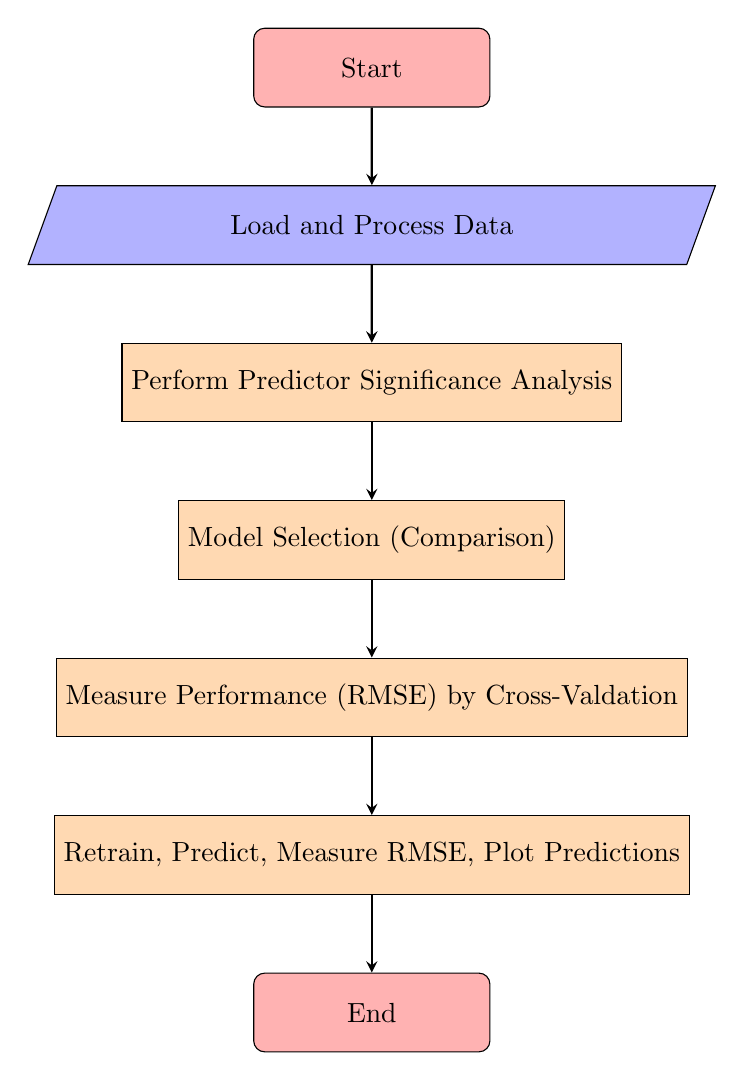
\begin{tikzpicture}[node distance=2cm]

\node (start) [startstop] {Start};
\node (data) [io, below of=start] {Load and Process Data};
\node (rf) [process, below of=data] {Perform Predictor Significance Analysis};
\node (modelSelect) [process, below of=rf] {Model Selection (Comparison)};
\node (kfold) [process, below of=modelSelect] {Measure Performance (RMSE) by Cross-Valdation};
\node (retrain) [process, below of=kfold] {Retrain, Predict, Measure RMSE, Plot Predictions};
\node (results) [startstop, below of=retrain] {End};

\draw [arrow] (start) -- (data);
\draw [arrow] (data) -- (rf);
\draw [arrow] (rf) -- (modelSelect);
\draw [arrow] (modelSelect) -- (kfold);
\draw [arrow] (kfold) -- (retrain);
\draw [arrow] (retrain) -- (results);
\end{tikzpicture}
\caption{Analysis approach}
\label{fig:analysis_approach}
\end{figure}

This schematic illustrates the general workflow in our data analyses from initial data loading and pre-processing, through feature importance analysis and model selection, to performance evaluation using k-fold cross-validation, and final model training and validation including visualization of predictions.
\newline

Before we move on: The first model will be walked through quite thoroughly in a step-by-step manner, to demonstrate the general approach and techniques we have used for the data analysis in this thesis. Subsequent models and analysis will be focus on demonstrating briefly the nature of the data, the challenges and complexities in modelling it, and the comparing the results obtained. The primary objective of the data analysis in this thesis is to demonstrate the viability of spline regression in typical data sets, and to determine if \texttt{glmmTMB} can be a good choice for specifying GAMMs with it's easy to use and flexible features like sub-models for dispersion and zero inflation, as well as a rich family of easily specified distributions.
\newline
\textbf{Disclaimer:} We are not experts in every (or any) of the domains of these particular analyses, and our models are not necessarily the most appropriate for the data. But as is mentioned in the introduction, one of the aspects of our analyses is to investigate to which degree easy inclusion of zero inflation, dispersion and specialized distributions can help non-experts develop better models. 


\subsection{Choice of Performance Metrics} 

We have found that for these complex models, the effectiveness of AIC as a metric for model performance is limited to guiding model tweaking in the experimental phase, particularly in the selection and refinement of model formulations and the combinations of explanatory variables in \textbf{linear} models (comparing nested models). Generally, in our experience, AIC has not been a good indicator of model performance, but rather to the contrary, lower AIC scores have in many cases resulted in overfitting, which we have seen manifested by larger prediction error on unseen data.

\paragraph{RMSE for Model Performance Evaluation.} Given the limitations of AIC in assessing model performance, we have opted for the use of RMSE as the primary metric for evaluating the effectiveness of models. RMSE offers a direct measure of a model's predictive accuracy by quantifying the average magnitude of the prediction errors across cross-validation folds and on unseen test data. This metric is quite useful, as it is directly interpretable in the context of the response variable's units, providing direct insights into the model's predictive capabilities. Ideally we would use \textit{true} test data external to the original data set, however, this is usually hard to obtain. Instead we opt for the typical approach of splitting the full datasets into training, validation and test sets. The models are rigorously evaluated through cross-validation (on the validation set) to aid model selection by assessment of their predictive power. Finally, the selected models are re-trained on the full data (excluding the test set) and evaluated by the RMSE of the predictions on the test data. This follows the standard and recommended practices outlines source here.
\textbf{Note:} For binary outcomes (logistic regression) we use the F1 score as our performance metric. Ideally we should perform further statistical tests on the results to determine whether the differences observed are statistically significant, or could be explained by chance. We will be taking a more "practical" approach and interpret the results based on the models and results as a whole.

\paragraph{Visual Assessment and Further Considerations.} In addition to RMSE, we try to provide informative plots and visuals comparisons. These offer an intuitive view and understanding of the model's predictive accuracy and highlight areas where improvements may be necessary. We will mainly provide \textbf{loess} regression lines and density plots of predictions vs actual values.

\subsubsection{Time Series and Forecasting Models}
Before our first analysis, we'll provide a bit of background on time series forecasting. Predicting financial trends is not easy, and for accurate results one is reliant on accessing as much information as possible, in order to maximize the probability of identifying patterns which are true signals in the midst of all the noise. Jim Simons, mathematician and Founder of one of the most successful hedge funds ever, Renaissance, says in this \href{https://english-online.hr/materials/42d8c0fe0de3cd0}{interview} that \textit{''We take in terabytes of data a day''}. Specifically, the firm possesses a research database expanding by more than 40 terabytes a day, 50,000 processing cores with 150 gigabits per second of global connectivity \citep{RenaissanceTech2024}.
\newline

We have made substantial efforts into ensuring that we have been careful and methodical in our data splitting, and have used appropriate cross-validation techniques, such as rolling or expanding windows with walk forward validation methods. We also make sure that any incorporation of engineered variables are done such as to minimize the risk of \textbf{look-ahead bias} or \textbf{information leakage} in the models. This we achieve by making sure our models have no access to information from future observations (or any information which would not have been available in a realistic forecasting setting), Such variables are only calculated from training data, and predicted/forecasted to the test data. Since, by definition, (random) variables can not be known ahead of time, we lag time specific variables appropriately. Further details can be found in \ref{sec:app:time_series} and full R code on \href{https://github.com/AllInCade/MasterProject}{GitHub}.
\newline

\textbf{Note:} Real Time Trading models are becoming increasingly utilized in finance and trading institutions, like high frequency trading hedge funds. They employ highly sophisticated models, but rely on the concepts of time series analysis fundamentally, just at an extreme level, where latency reduction and run time optimization are of upmost importance (models are often run on "bare metal"  implementations, i.e directly on hardware). 

\subsection{Financial Data}\label{sec:analysis:timeseries}
Many financial markets are characterized by inherent volatility and complex, non-linear dynamics. In such circumstances, flexible spline models can be a viable choice in modelling and predicting the behaviour of the market. 
\newline

That being said, stock prices and markets can be (and are) influenced by a all sorts of factors which are (practically) impossible to include (and predict), and are thus are inherently unpredictable, particularly on a day-to-day basis. This is actually a fundamental properties of well-behaved markets under the \textit{"Efficient Market Hypothesis"}. The assumptions the EMH are not met in the real world markets however, and there are techniques and methods that allow us to identify trends and patterns, which can be used to predict future trends with some degree of accuracy (but with significant uncertainty). 


\begin{figure}
\begin{center}
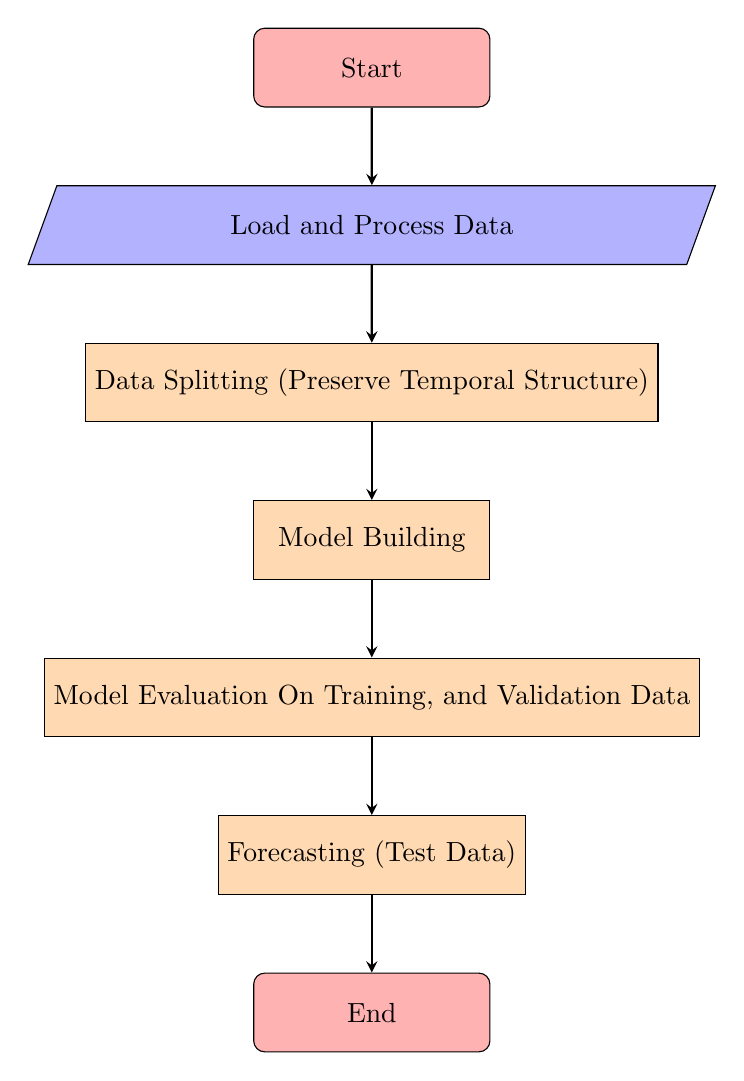
\begin{tikzpicture}[node distance=2cm]
\node (start) [startstop] {Start};
\node (data) [io, below of=start] {Load and Process Data};
\node (split) [process, below of=data] {Data Splitting (Preserve Temporal Structure)};
\node (model) [process, below of=split] {Model Building};
\node (evaluate) [process, below of=model] {Model Evaluation On Training, and Validation Data};
\node (forecast) [process, below of=evaluate] {Forecasting (Test Data)};
\node (end) [startstop, below of=forecast] {End};

\draw [arrow] (start) -- (data);
\draw [arrow] (data) -- (split);
\draw [arrow] (split) -- (model);
\draw [arrow] (model) -- (evaluate);
\draw [arrow] (evaluate) -- (forecast);
\draw [arrow] (forecast) -- (end);
\end{tikzpicture}
\caption{Model Flow}
\label{fig:Model_flow}
\end{center}
\end{figure}

This figure illustrates a general outline of the sequential steps involved in our analyses in simple terms. 

\subsubsection{Log Return I}\label{sec:analysis:timeseries:model}

For this analysis we'll fit a linear model and a GAM, using the \texttt{glmmTMB} package. We will be modelling the log-returns of the "big five indicators" of the global economy, which are the following: Dow Jones Industrial (DJI), S\&P 500 (GSPC), Nasdaq 100 (NDX), HANG SENG Index (HSI) and the FTSE 100 (FTSE). The primary objective is to investigate the differences between a spline based model and a linear model on this type of data. Although log returns are designed to linearize and normalize the data, other assumptions of a linear model may not be met.
\newline

We import up-to-date data from Yahoo Finance using the \texttt{Quantmod} package for R. We filter select data from 2014-01-01 and up to the latest available date, which is typically one trading day prior to the current date, in this case late march / early April. 

The final two models are as specified below

\begin{lstlisting}[language=R]
lm(log_ret~ time + volume + close_open_ratio +
               rsi_20 + sma_20 + hist_vol_20 +
               trend + seasonal
               trend,
               data = current_train_data€

glmmTMB(log_ret ~ s(time€ + s(volume€ + 
            s(close_open_ratio€ +
            s(rsi_20€ + s(sma_20€ + s(hist_vol_20€ +
            s(trend€,
            disp =~ month,
            data = current_train_data,
            family = gaussian(link = "identity"€,
            REML = TRUE€
\end{lstlisting}

\subsubsection*{Data Preparation and Engineering}

After the loading the data we perform the necessary pre-processing steps ensuring that the variables are formatted correctly. We define a time variable by ordering the data frame by the time series object index. We'll also define a month and day of week variable, as there may be some seasonal and week-day based patterns. 
\newline

The data is split into training and validation sets, while preserving the temporal structure (maintaining chronological order). 
\newline

We use tools form the \texttt{TTR} package to engineer relative strength index (RSI), simple moving average (SMA) and historical volatility (runSD) variables for our analysis. Additionally, we do a time series decomposition to extract trend and seasonal components. This engineering is performed carefully to avoid any look-ahead or information leakage. The variables are lagged by one observation, so that the model only has information available which can be known in a realistic setting. Example code in \ref{sec:app:time_series}.


\subsubsection{Model Selection}

Since we're accessing just the data included in the \texttt{quantmod} time series object for the particular symbol, our model is quite limited. We have made sure no information has been available to the model which couldn't have accessed ahead of time in a real world scenario. Volume, close to open ratios, the time series components and the market indicators RSI, SMA and historical volatility may provide sufficient information for the model to predict with reasonable efficiency the main body of the target distribution, but the larger values (big market swings / movements) are nearly entirely missed. This is not surprising, as the information available to the model should account for the typical trading and periodic patterns seen in financial data, but large swings are usually the result of external factors like market sentiments, commodity prices, geopolitical uncertainty (wars etc), real-estate crisis, central bank failures, pandemics or political / financial policy changes, which we have not included for our analysis. 

\subsubsection{Results}

By the results we obtained here, it's clear that we are lacking information (data) to accurately predict future log returns, and although we have incorporated engineered variables to manage autocorrelation, a GARCH or ARIMA(X) model is likely more suitable for this type of data. For these quite simple and naive models, there doesn't seem to be any advantage in using smooth terms as opposed to linear terms in the predictor set. In the next section we'll try construct a better model in a more thought-out analysis. 

\begin{table}[H]
\centering
\caption{Model Evaluation Results}
\label{table:model_evaluation}
\begin{tabular}{lcc}
\hline
\textbf{Model} & \textbf{Symbol} & \textbf{Avg. validation RMSE} \\
\hline
Linear & DJI & 0.0097 \\
GAM & DJI & 0.0089 \\
Linear & GSPC & 0.0108 \\
GAM & GSPC & 0.0109 \\
Linear & NDX & 0.0138 \\
GAM & NDX & 0.0151 \\
Linear & HSI & 0.0145 \\
GAM & HSI & 0.0147 \\
Linear & FTSE & 0.0087\\
GAM & FTSE & 0.0076 \\
\hline
\end{tabular}
\end{table}

\subsection{Log Return II}\label{sec:analysis:alt_mod}

Since we've established that predicting log returns (and financial assets in general) is quite difficult, and may require access to more data than is typically \textit{easily} available, we will now try to create a model using more data than in the previous attempt, and potentially in a more clever way. 
\newline

Since on any given day, Japan gets to wake up before Europe, the Japanese market opens and closes before the European one(s). And particularly since the Japanese market closes before the European ones open, and our data is recorded daily at closing, we can try and use the information from today's movements in the Japanese market to inform us and predict the movements in the European ones for that day. 

\subsubsection{Merged Datasets}
We import the data from the Nikkei 225 Index (N225) and try to predict the log return of the Euronext 100 Index (N100) by forecasting the log return of the Nikkei 225 of that day. Ideally we would use much more data than this, but, while joining and merging multiple time series objects and vast data tables, lagging each appropriately etc, is doable, it's quite a lot of work and it's beyond the scope of our analysis here.

We merge the N225 and N100 data, and make sure the N100 data is lagged by 1 observation so it only contains information available before time $t$. The N225 data does not need to be lagged, since its information at time $t$ (current day) is available before time $= t$ for the response variable \texttt{N100.log\_return}. That is, current day information from the Japanese market is available before the European market opens and thus we can use it. Due to the limited amount of extra information, and the inherent unpredictability of daily swings, we shouldn't expect more than marginal improvements. That is not say that if given enough information, utilized in a sufficiently intelligent way, we couldn't increase the accuracy of our predictions. Usually it's hard to deduce the best model simply from theoretical foundations, and one has to resort to simply just trying lot's of different configurations and see which works best for any given task.

\subsubsection{Model Selection}

As before we calculate indicators like RSI, SMA and historical volatility. We set a forecasting horizon of one day, since we are simulating a situation where we make predictions about the log return for the N100 index for the current day, before it opens. We'll compare linear models vs GAMs, with and without N225 data. The length of time for the indicators are experimented with. After performing a feature importance analysis we identify the most significant predictor, such as the previous days' N100's log return, today's N225 log return, the RSI of each index, among a few others. After some experimentation we arrive at the following models:
\newline

Only N100 data 
\begin{lstlisting}[language=R]

lm(log_ret ~ time + 
                N100_RSI_lag + 
                N100_trend +
                N100_log_ret_lag,
                data = train_data€

glmmTMB(log_ret ~ s(time€ +
                   N100_log_ret_lag + 
                   s(N100_RSI_lag€ + 
                   s(N100_trend€,
                   disp =~ 1,
                   data = train_data,
                   family = gaussian(€, 
                   REML = TRUE€
\end{lstlisting}

Combined N100 and N225 data

\begin{lstlisting}
lm(log_ret ~ time + 
            N100_RSI_lag + N100_trend +
            N100_log_ret_lag + N225_RSI +
            N225_log_ret,
            data = train_data€

glmmTMB(log_ret ~ s(time€ +
                N100_log_ret_lag + 
                s(N100_RSI_lag€ + N225_log_ret +
                s(N100_trend€ + s(N225_RSI€,
                disp =~ N100.Adjusted_lag,
                data = train_data,
                family = gaussian(€, 
                REML = TRUE€
\end{lstlisting}


\subsubsection{Results}

The table below contains the average RMSE of 1 day forward forecasts on the log returns of the Euronext 100 Index. The data is collected from 2020-01-01 to 2024-04-01. There is a 4:1 train to validation set ratio. All the market indicators are calculated on a 20 day basis (4 weeks). The method of validation is an expanding windows cross validation, which resembles a daily accumulation of information.

\begin{table}[H]
\centering
\caption{Average RMSE for Different Models and Data Sets}
\label{tab:rmse_comparison}
\begin{tabular}{@{}lcc@{}}
\toprule
Model & Merged Data & Average RMSE \\ 
\midrule
Linear & no & 0.0055 \\ 
GAM & no &  0.0054 \\ 
Linear & Yes & 0.0056 \\ 
GAM & Yes & 0.0052 \\ 
\bottomrule
\end{tabular}
\end{table}

\begin{figure}[H]
    \centering
    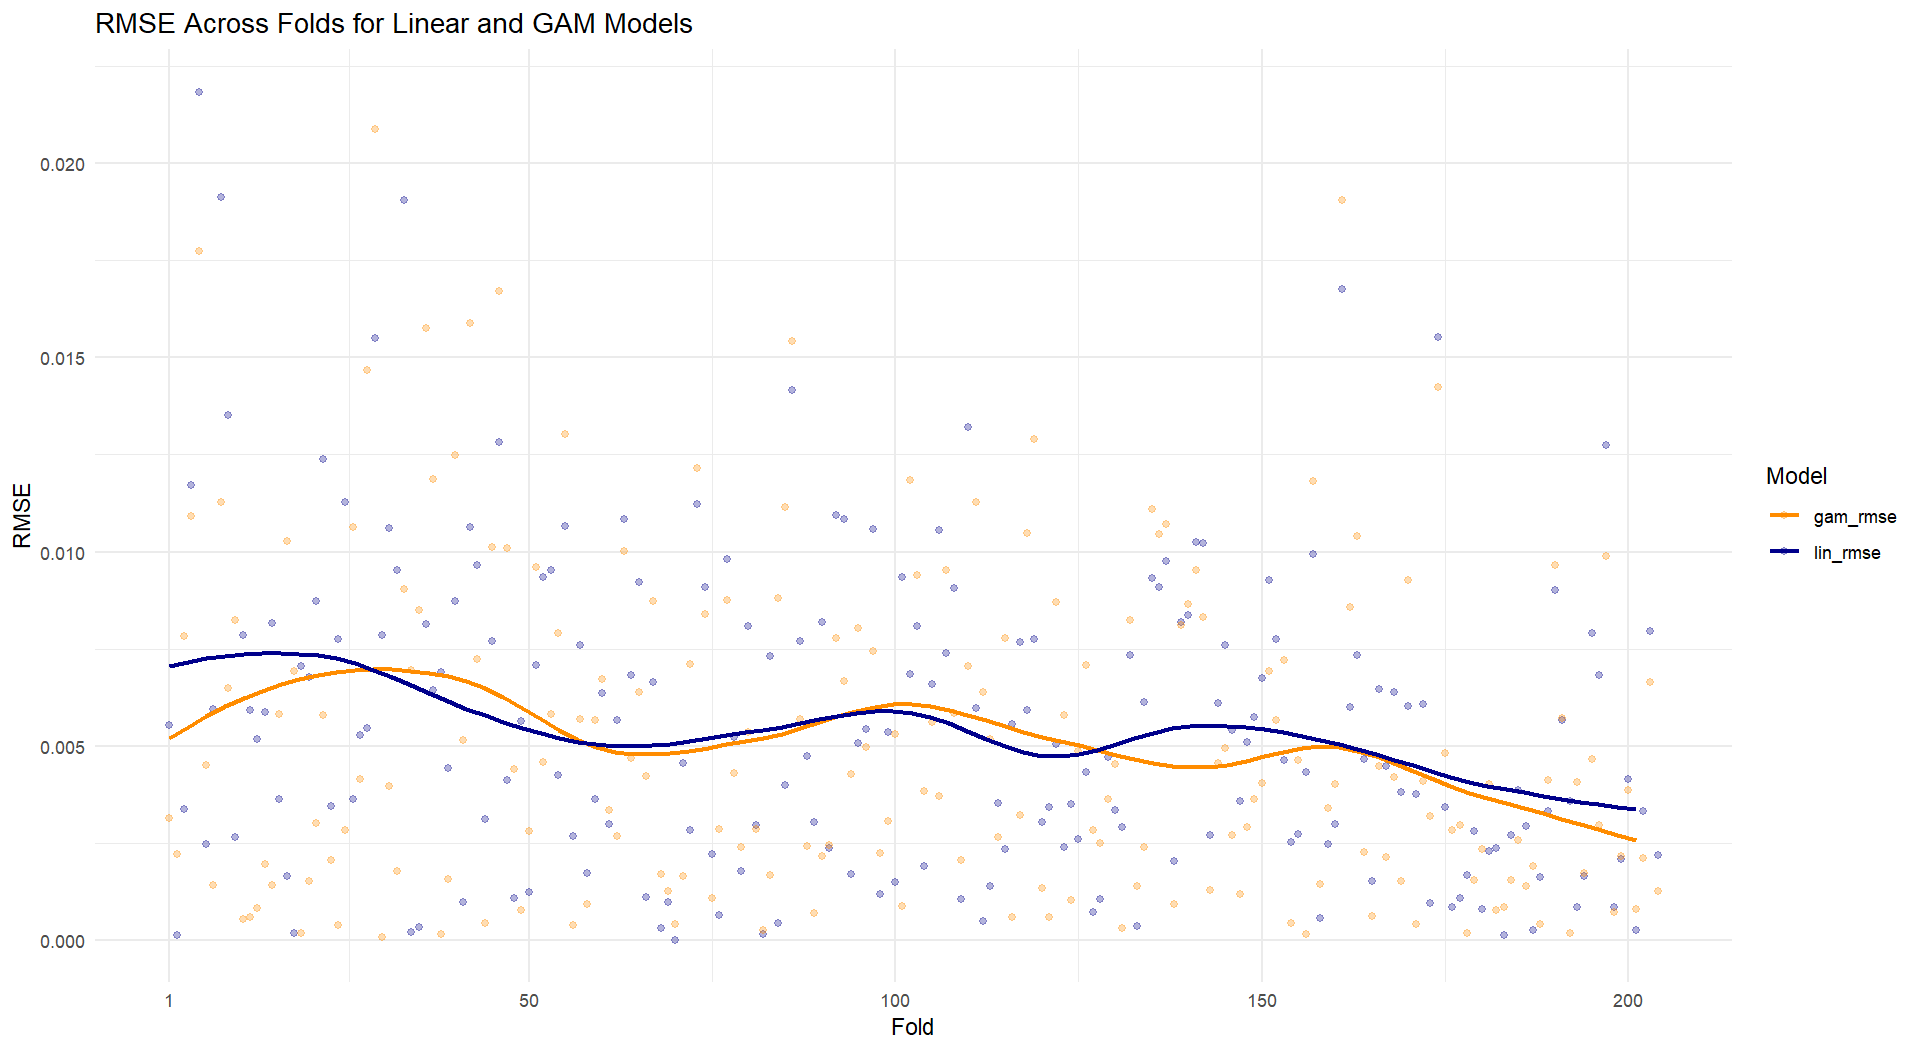
\includegraphics[width=\linewidth]{visuals/log_return/rmse_folds_lr2.png}
    \caption*{RMSE over folds (days) (lower is better).}
    \label{log_return_alt_rmse_folds}

    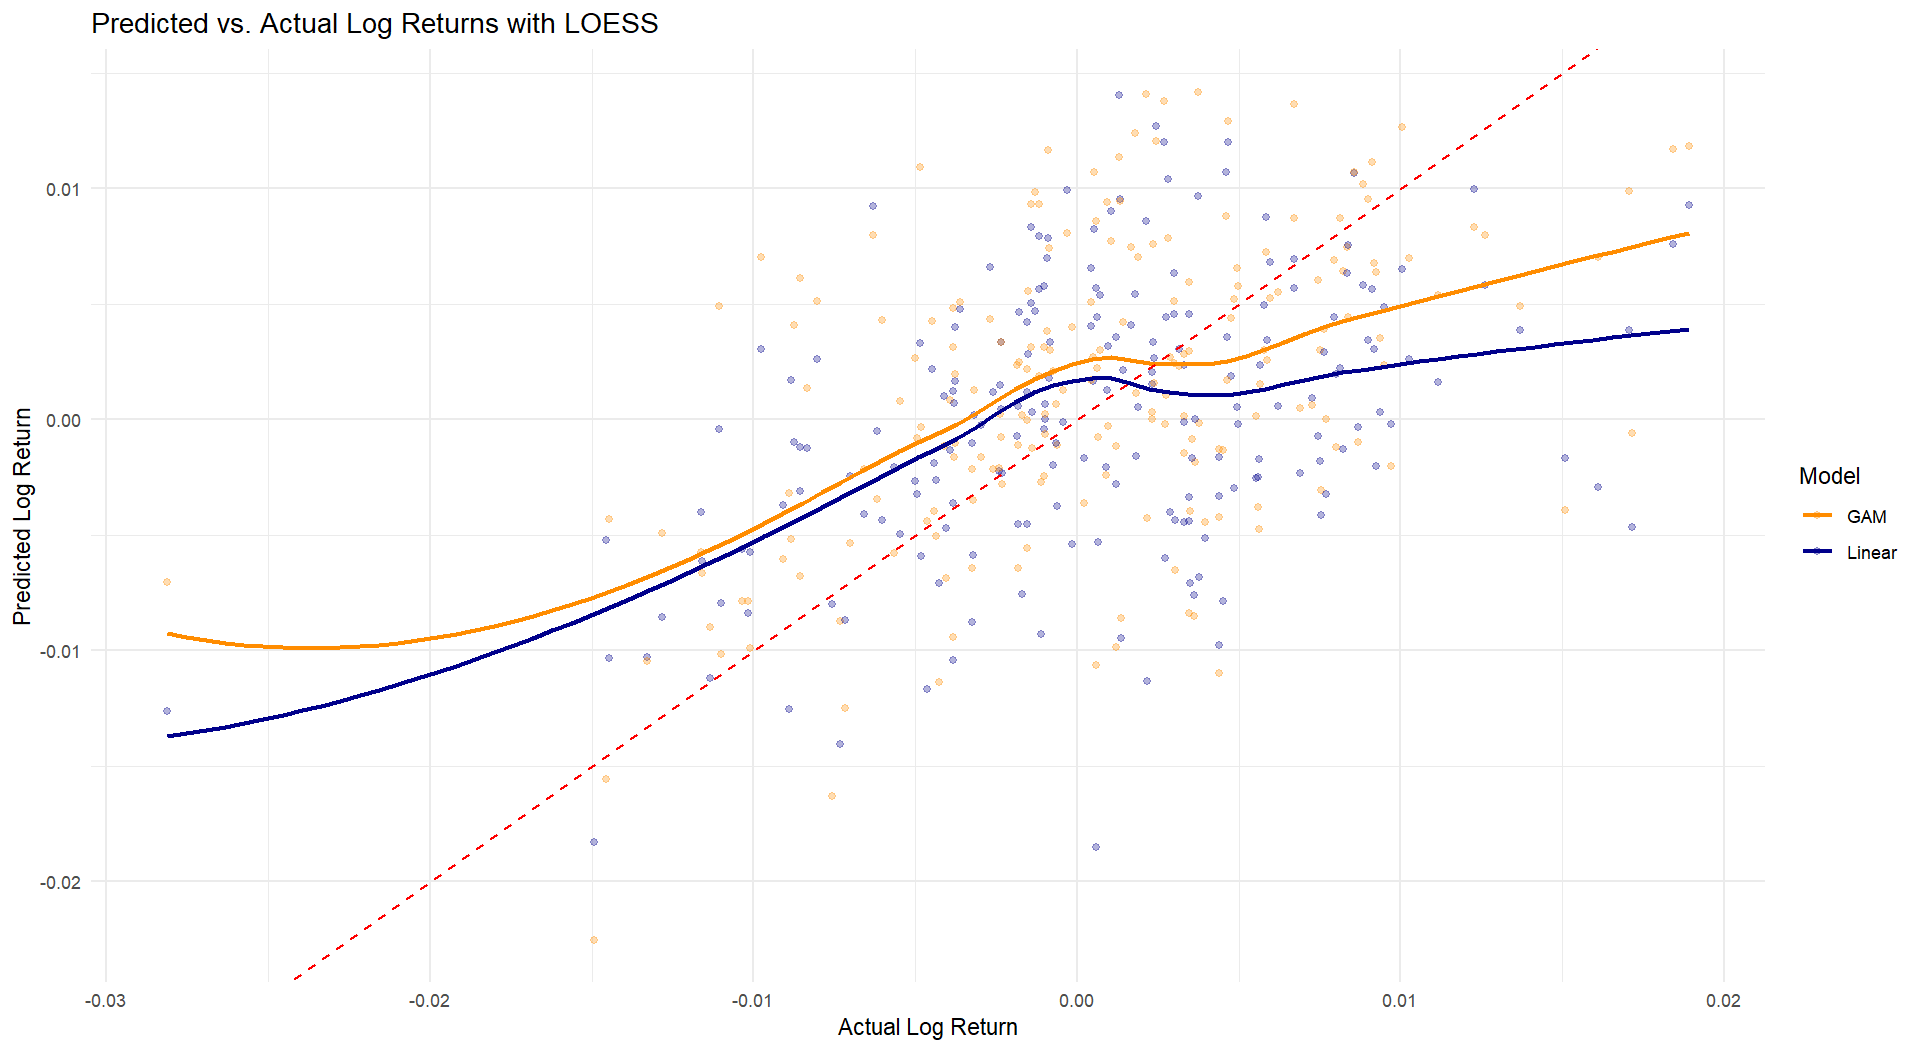
\includegraphics[width=\linewidth]{visuals/log_return/lr2_loess_bige_and_wide.png}
    \caption*{Loess regression line predicted vs actuals.}
    \label{log_return_alt_loess}

    \caption{Test Data Performance for Log Returns.}
    \label{results:log_return_alt}
\end{figure}

We observe consistent improvements with using smooth terms and including more data. A dispersion sub model slightly reduced the RMSE score as well for the GAM. The choice of training period and split ratio is somewhat arbitrary, and we would ideally cross validate over, or sample from, a large variety of time periods and data splits. For a more general model, we would ideally test the performance on more symbols as well. But in conclusion we do obtain much better results with this more sophisticated model, compared to the previous attempt in \ref{sec:analysis:timeseries:model}.

\subsection{Bank Failures Count}\label{sec:analysis:bank_fail_count}

\textbf{Note:} For this and all the following models in this chapter, we will primarily compare \texttt{glmmTMB} against \texttt{gamm4} for GAM(M) models, or against linear models. We've already established that for simple Gaussian GAMs, the two frameworks tend to produce the same outputs. Due to differences in optimizations routines. numerical procedures, parameterizations of package specific distribution families and so on, we shouldn't expect all types of models to be exactly equal.

\paragraph{Bank Failure Data}
This dataset comprises records of bank failures, compiled by The Federal Deposit Insurance Corporation (FDIC). We'll use it to analyze the factors influencing these financial institutions' stability. Each entry in the dataset represents a unique incident of bank failure, identified by a unique identifier (\textit{ID}), spanning from 1975 to 2024 (you can choose the time period on the site). The dataset includes several key variables, and you can find all the details \href{https://banks.data.fdic.gov/explore/failures?aggReport=detail&displayFields=NAME%2CCERT%2CFIN%2CCITYST%2CFAILDATE%2CSAVR%2CRESTYPE%2CCOST%2CRESTYPE1%2CCHCLASS1%2CQBFDEP%2CQBFASSET&endFailYear=2024&sortField=CERT&sortOrder=asc&startFailYear=1975}{here}.


\subsubsection{Counts of Bank Failures}

We'll begin with a model designed to analyze bank failures. The data is of the type \textit{event log} - a record of occurrences where each entry signifies an event of interest, in this case, a bank failure. We engineer our response variable, \textit{FailuresCount}, to count the number of bank failures observed on days when at least one failure is recorded. That is, we're making a counting model. When working with count data models we have to be mindful of the mean-variance relationship. Most straight forward count models assume a Poisson distribution, which has the property that the variance is equal to the mean. In many situations this is not actually the case. We'll investigate this in the model selection phase. 

\subsubsection{Model Selection}
First we compare a simple Poisson model: 

\begin{lstlisting}[language=R]
glmmTMB(FailuresCount ~ s(TIME€  + (1|STATE€,
                data = bank_data_full, 
                family = poisson,
                REML = TRUE)


gamm4(FailuresCount ~ s(TIME€, 
                random = ~(1 | STATE€,
                data = bank_data_full, 
                family = poisson,
                REML = TRUE€ 
\end{lstlisting}

We'll outline some of the basic pre-processing steps we've performed. Full code on \href{https://github.com/AllInCade/MasterProject}{Github}.

\begin{itemize}
    \item FAILDATE formatted by as.date (m, d, Y).
    \item Create the FailuresCount variable by aggregate(ID ~ FAILDATE), which counts how many banks failed on a given day (recall there are no zero count entries in the data by definition). 
    \item TIME variable is created from the FAILDATE variable. 
    \item CTIYST is split into separate CITY and STATE variables by strsplit on comma delimiter.
    \item Create WEEKDAY variable from FAILDATE and \texttt{wday()}. 
\end{itemize}

The two Poisson models are very approximately equal. A dispersion test shows that there is significant overdispersion. And a quick check of the mean and variance of the response variable confirms this as well, with the mean being about 7.9 and the variance 156. This suggests the mean-variance relationship is likely quadratic in nature, rather than linear, hence we'll use the \texttt{nbinom2} distribution for the \texttt{glmmTMB} model. For the \texttt{gamm4} model we'll use the negbin family with lower values for theta. We continue to add random effects that are significant in explaining the \texttt{FailuresCount}, and finally we fit a dispersion sub model to the \texttt{glmmTMB} model. 

Through some testing we arrive at the following best performing models for each framework

\begin{lstlisting}[language=R]
glmmTMB(FailuresCount ~ s(TIME€ + s(YEAR€ + 
            s(MONTH€ + (1|STATE€ + 
           (1|SAVR€ + (1|CHCLASS1€ + 
           (1|RESTYPE1€,
           dispformula =~ RESTYPE + WEEKDAY,
           data = train_fold, 
           family = nbinom2(link="inverse"€,
           REML = TRUE€

gamm4(FailuresCount ~ s(TIME€ + s(YEAR€ + s(MONTH€, 
         random =~ (1|STATE€ + (1|SAVR€ + 
         (1|CHCLASS1€ + (1|WEEKDAY€ + 
         (1|RESTYPE€,
         data = train_fold, 
         family = negbin(theta=2€,
         REML = TRUE€
\end{lstlisting}

\subsubsection{Results}

As evident by the RMSE scores, the \texttt{glmmTMB} framework performed best here. It's likely possible to get similar results using \texttt{gamm4}, but we attribute the more successful model fit here to the ease of implementing a dispersion sub model and the \texttt{nbinom2} parameterization of the negative binomial distribution, as these are the only (other than optimization routines) differences between the models. Efforts were made to equalize the models w.r.t to the optimizer and start values, but we had difficulties managing the control options in \texttt{gamm4}, which seem less flexible than in \texttt{glmmTMB}. 
From figure \ref{fig:test_data_performance_2} the \texttt{glmmTMB} model outperforms the \texttt{gamm4} one, which fails almost entirely to predict the higher range of values. We can see that
while the \texttt{glmmTMB} model does a decent job in predicting the higher values, it also suffers from some degree of underestimation. It's reasonable to expect that predicting large scale bank failure events requires more information than what is available in the data we have at hand. 

\begin{table}[H]
\centering
\caption{Model Evaluation Results}
\label{table:model_evaluation}
\begin{tabular}{lcc}
\hline
\textbf{Model} & \textbf{Cross Validation RMSE} & \textbf{Test Data RMSE} \\
\hline
gamm4 & 10.607 & 11.560 \\
glmmTMB & 7.915 & 7.404 \\
\hline
\end{tabular}
\end{table}

\begin{figure}[H]
    \centering
        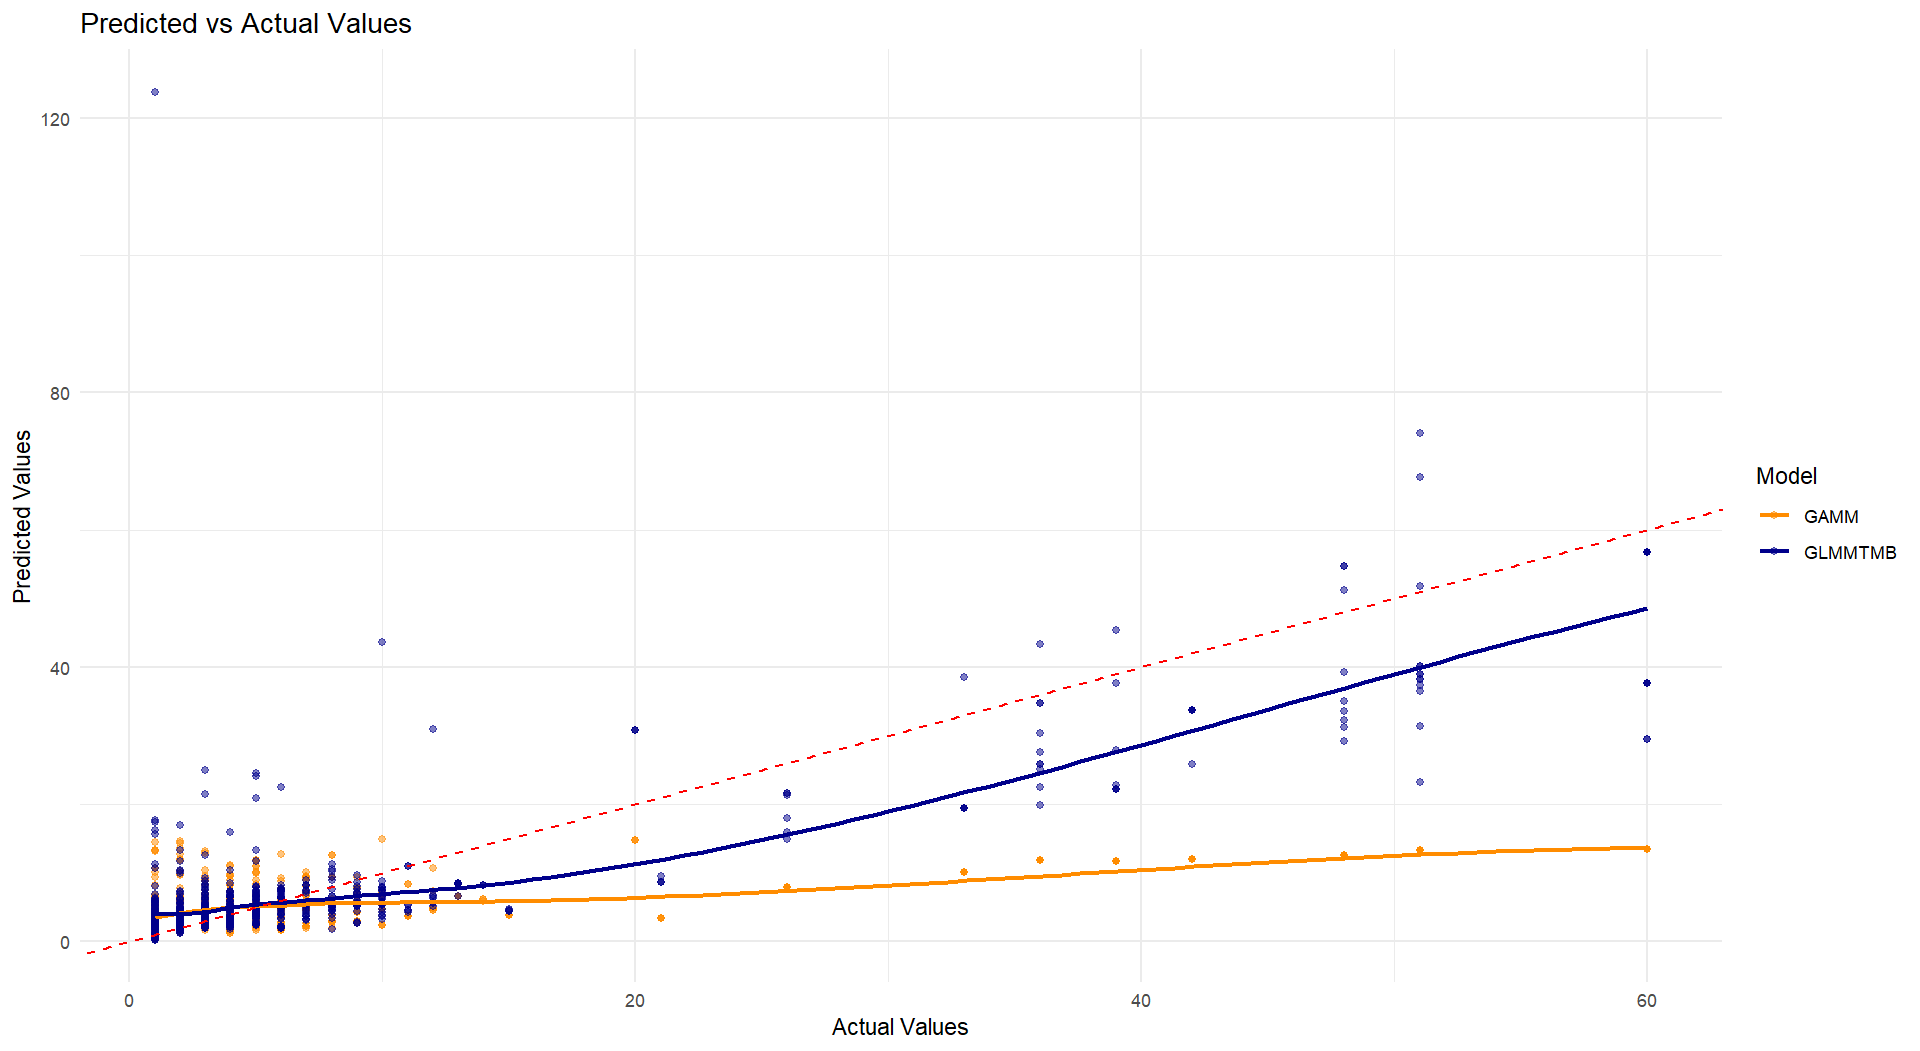
\includegraphics[width=\textwidth]{visuals/Bank_fail_count/pred_vs_acutal_fail_count_loess.png}
        \caption*{Predicted values vs actual values plotted and smoothed by loess regression. }
        \label{fig:hist_pred_errors}

        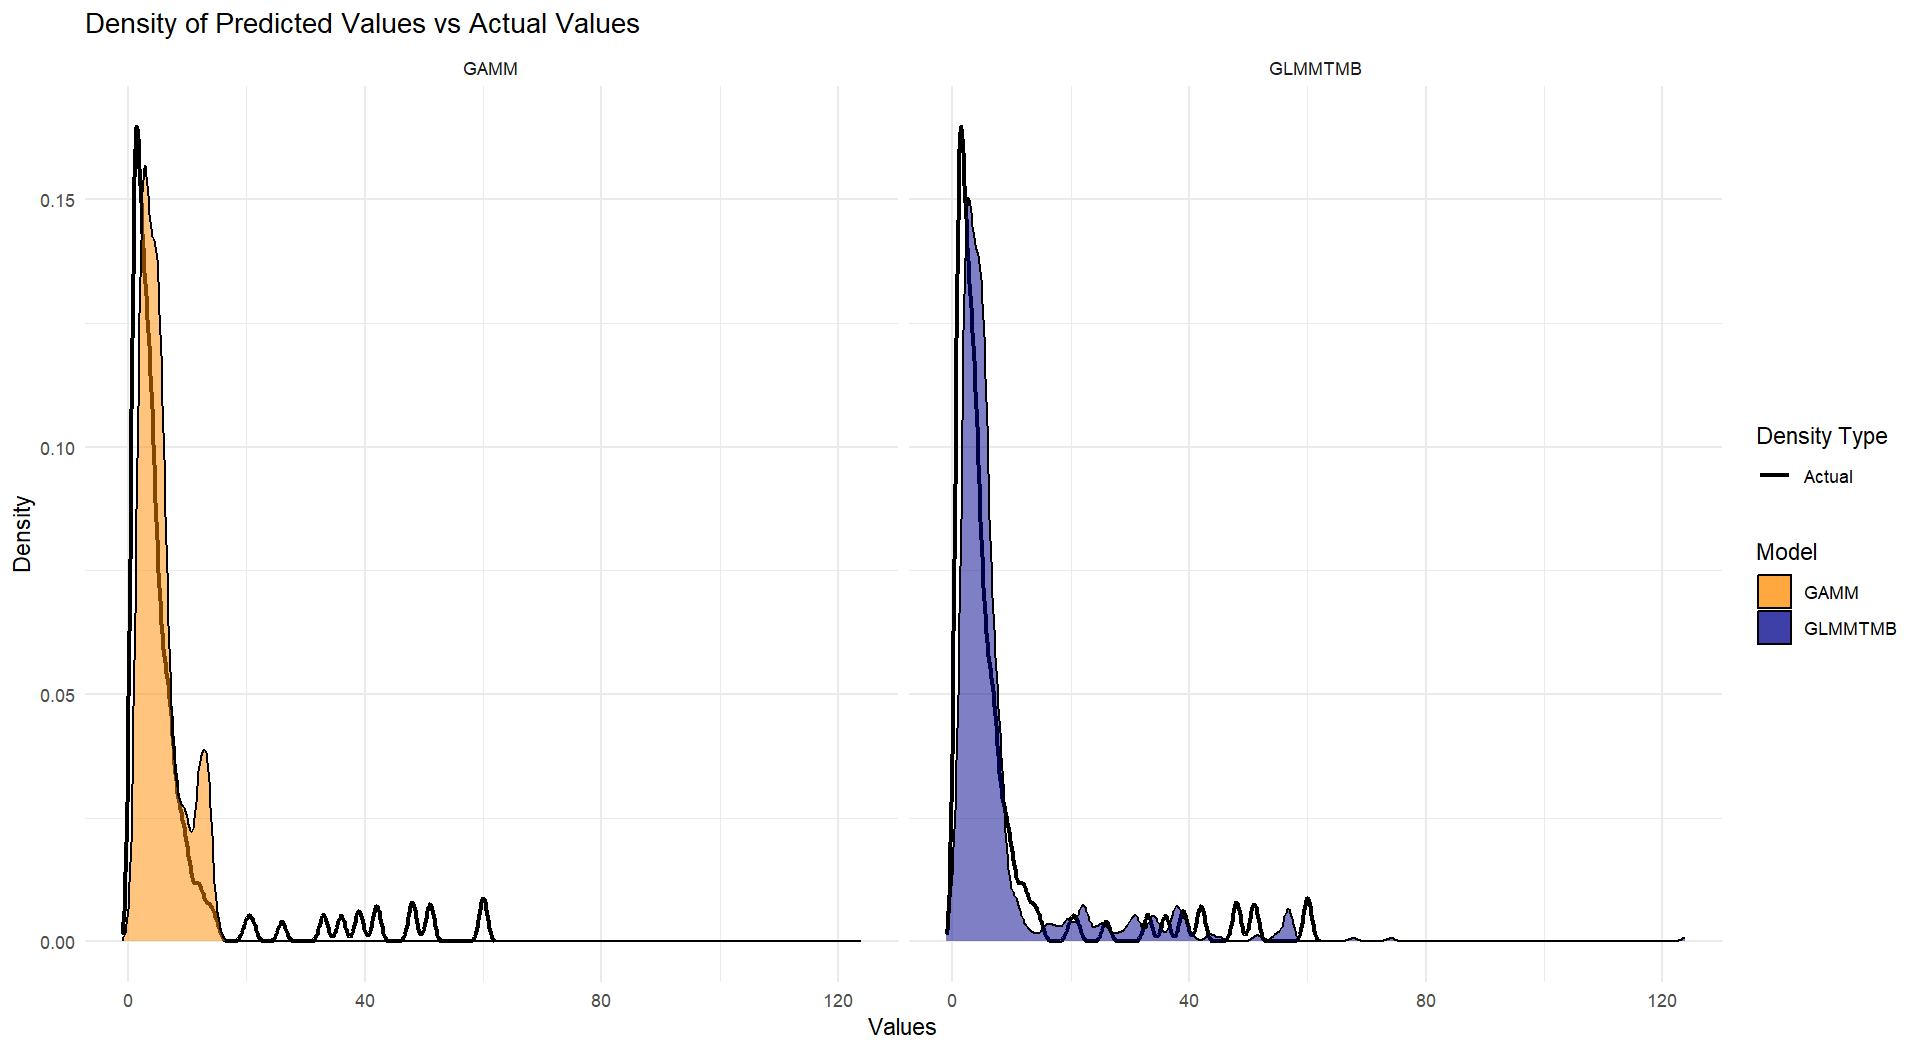
\includegraphics[width=\textwidth]{visuals/Bank_fail_count/pred_vs_actual_fail_count_density.png}
        \caption*{Predicted vs Actual Densities}
        \label{fig:predicted_vs_actual_densities}

    \caption{Test Data Performance Bank Failures.}
    \label{fig:test_data_performance_2}
\end{figure}


\subsection{Bank Failures and Estimated Loss}\label{sec:analysis:bank_fail_cost}

Using the same dataset as above, we'll try predicting the COST (estimated loss) of a given bank failure. We'll assume a Gaussian model is an appropriate starting point, despite the fact that this type of data often has heavier tails than a normal distribution. It's probably safe to assume that total assets and total deposits are highly correlated with the estimated loss. Due to the extreme range of magnitudes in these three numeric variables (COST, QBFASSET, QBFDEP), some scaling or transformation is likely needed to help normalizing the distribution and ensure numerical stability, specially for the smooths. There are some negative values in the COST variable, which we won't consider or try to explain here, so we'll filter the data to only contain non-negative values for the response. This means means we can use a standard log + 1 transformation to the response, and the two other aforementioned numeric variables. Again, the details can found on \href{https://github.com/AllInCade/MasterProject}{Github}. 
\textbf{Note:}It's worth investigating how closely assets and deposits are correlated with each other (collinearity). Inspecting the dataset we can see that they are on average quite close, but there is a lot of apparent randomness in the assets to deposits relationship, so it doesn't seem to be a significant problem. However, in the second part of the paper, we will try Ridge regularized models, which are known to handle multicollinearity well.

\subsubsection{Model selection}

We begin with a simple formula to compare a linear model vs a GAM: 

\begin{lstlisting}[language=R]
glmmTMB(log_COST ~ TIME + log_DEPOSIT + 
                  log_ASSET, 
                  data = bank_data€
  
glmmTMB(log_COST ~ s(TIME€ + s(log_ASSET€ +     
                  s(log_DEPOSIT€,
                  data = bank_data, 
                  family = gaussian(link = "identity"€,
                  REML = TRUE€ 
\end{lstlisting}

An AIC comparison shows favorable results for the GAM with 11360 (GAM) vs 11548 (LM). 
\newline

Further experimenting with model formulas lead us to the following GAMMs: 

\begin{lstlisting}[language=R]
glmmTMB(log_COST ~ s(TIME€ + s(log_ASSET€ + 
                    s(log_DEPOSIT€
                    + (1|YEAR€ + (1|STATE€ + 
                    (1|CHCLASS1€,
                    dispformula =~ SAVR + RESTYPE,
                    data = train_data, 
                    family = gaussian,
                    REML = TRUE€

gamm4(log_COST ~ s(TIME€ + s(log_ASSET€ +       
                    s(log_DEPOSIT€,
                    random =~ (1|YEAR€ + (1|STATE€ + 
                    (1|CHCLASS1€,
                    data = train_data, 
                    family = gaussian(€, 
                    REML = TRUE€
\end{lstlisting}

As you can see the two models are equal except for the dispersion submodel included in the \texttt{glmmTMB} model. One thing to note when using random effects in models and predictions in cross validation, is that there may be test folds which do not contain any of entries of a particular level present in the training data. This can be handled by setting "allow.new.levels=TRUE" in \texttt{glmmTMB}. 
For the final model, we used a student's t distribution to try and capture more of the extreme values (further from the mean). This yielded a slight improvement over a Gaussian distribution. 

\subsubsection{Results}

\begin{table}[H]
\centering
\caption{Model Evaluation Results}
\label{table:model_evaluation}
\begin{tabular}{lcc}
\hline
\textbf{Model} & \textbf{Cross Validation RMSE} & \textbf{Test Data RMSE} \\
\hline
gamm4 & 1.381 & 1.206 \\
glmmTMB & 1.363 & 1.172 \\
\hline
\end{tabular}
\end{table}


\begin{figure}[H]
    \centering
        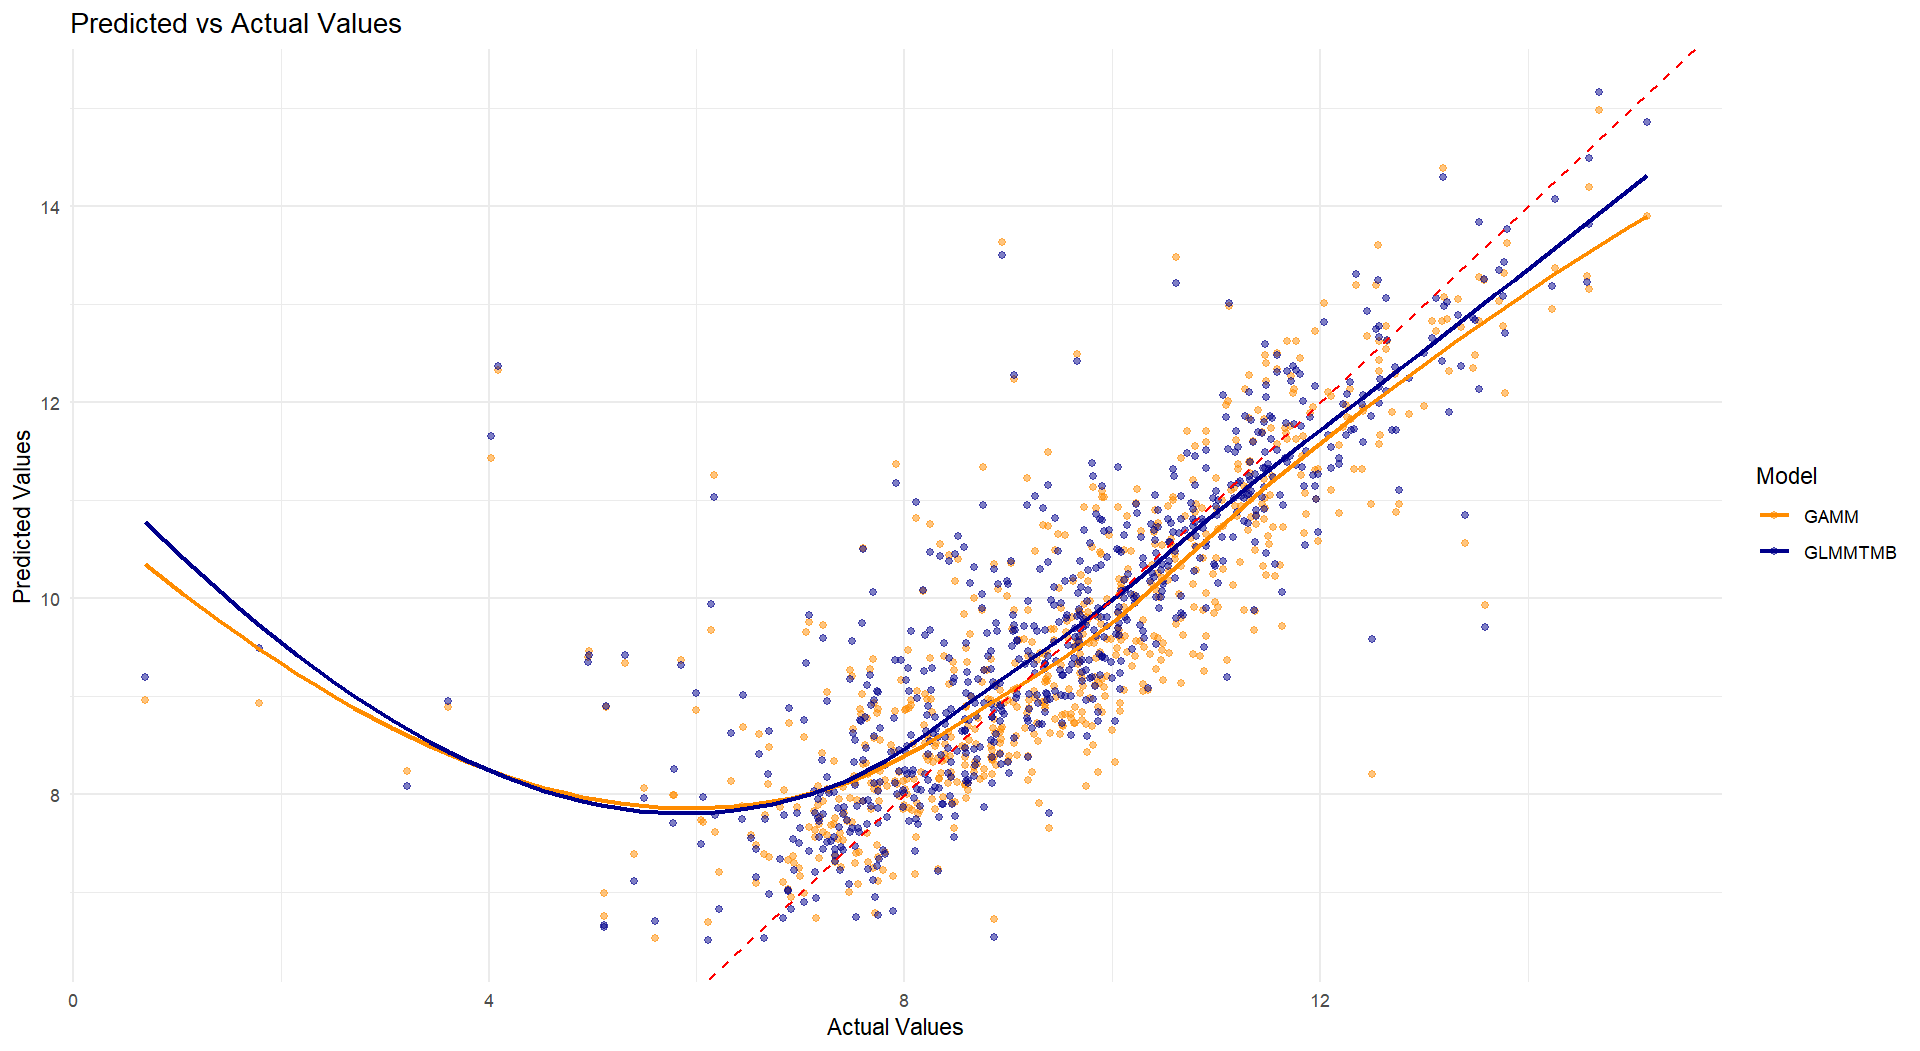
\includegraphics[width=\textwidth]{visuals/Bank_fail_cost/Pred_vs_actuals_loess.png}
        \caption*{Predicted values vs actual values plotted and smoothed by loess regression. }
        \label{fig:hist_pred_errors}

        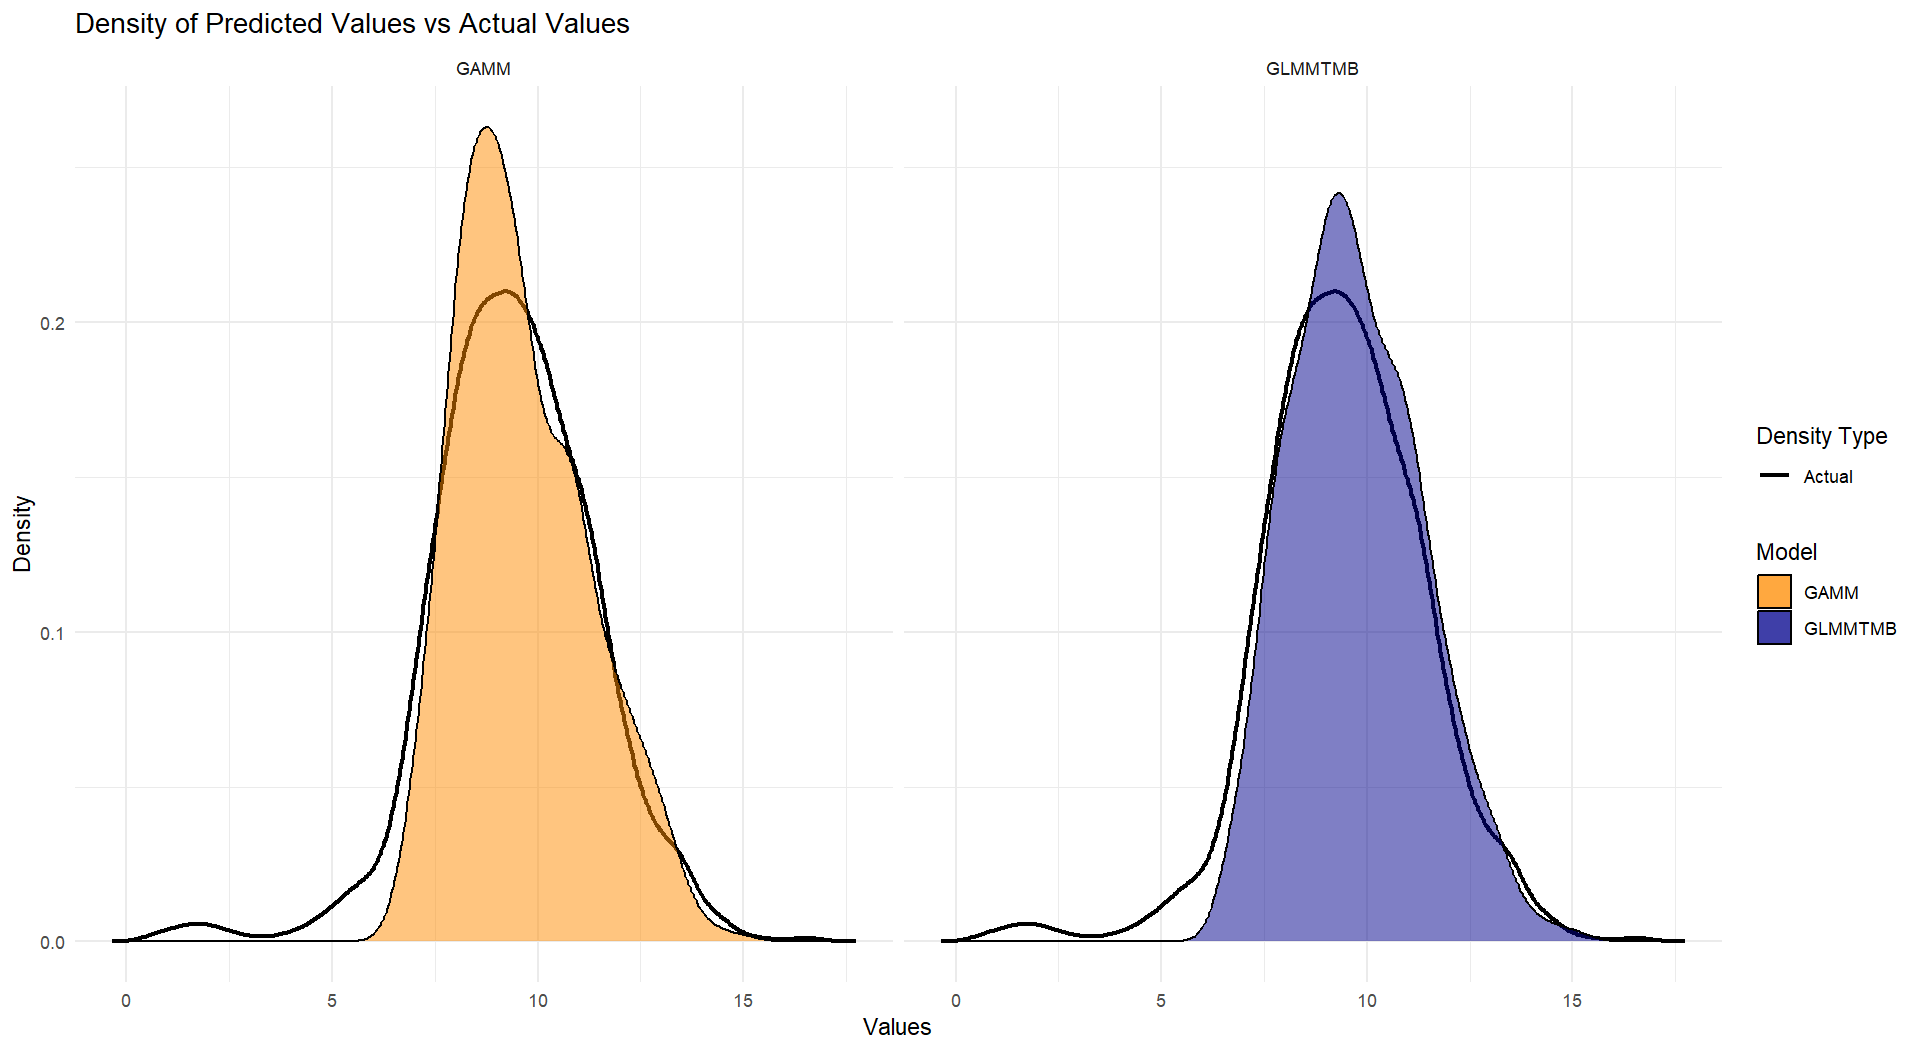
\includegraphics[width=\textwidth]{visuals/Bank_fail_cost/pred_vs_acutal_density.png}
        \caption*{Predicted vs Actual Densities}
        \label{fig:predicted_vs_actual_densities}

    \caption{Test Data Performance Log Cost.}
    \label{fig:test_data_performance_3}
\end{figure}


As the RMSE scores and the visuals show, the inclusion of a dispersion sub model and student's t distribution helped the \texttt{glmmTMB} model predict the extreme values slightly better.


\subsection{Hot and Cold Deviations Classifier}\label{sec:domains:weatherdata}\label{sec:analysis:sig_temp_anomalies}

The Weather Anomalies dataset comprehensively documents temperature deviations from historical norms from 1964 to 2013, utilizing data from various weather stations. This dataset merges raw observations from the National Oceanic and Atmospheric Administration (NOAA) with enhanced metrics derived from Enigma's weather analyses. In figure \ref{fig:heatmap_usa} we highlight coastal regions' warmer deviations and continental areas' cooler deviations. This pattern, known as continentality, features more significant temperature fluctuations—warmer summers and colder winters—inland compared to the moderated temperatures near coastlines, influenced by more stable ocean temperatures.

\begin{figure}[H]
\centering
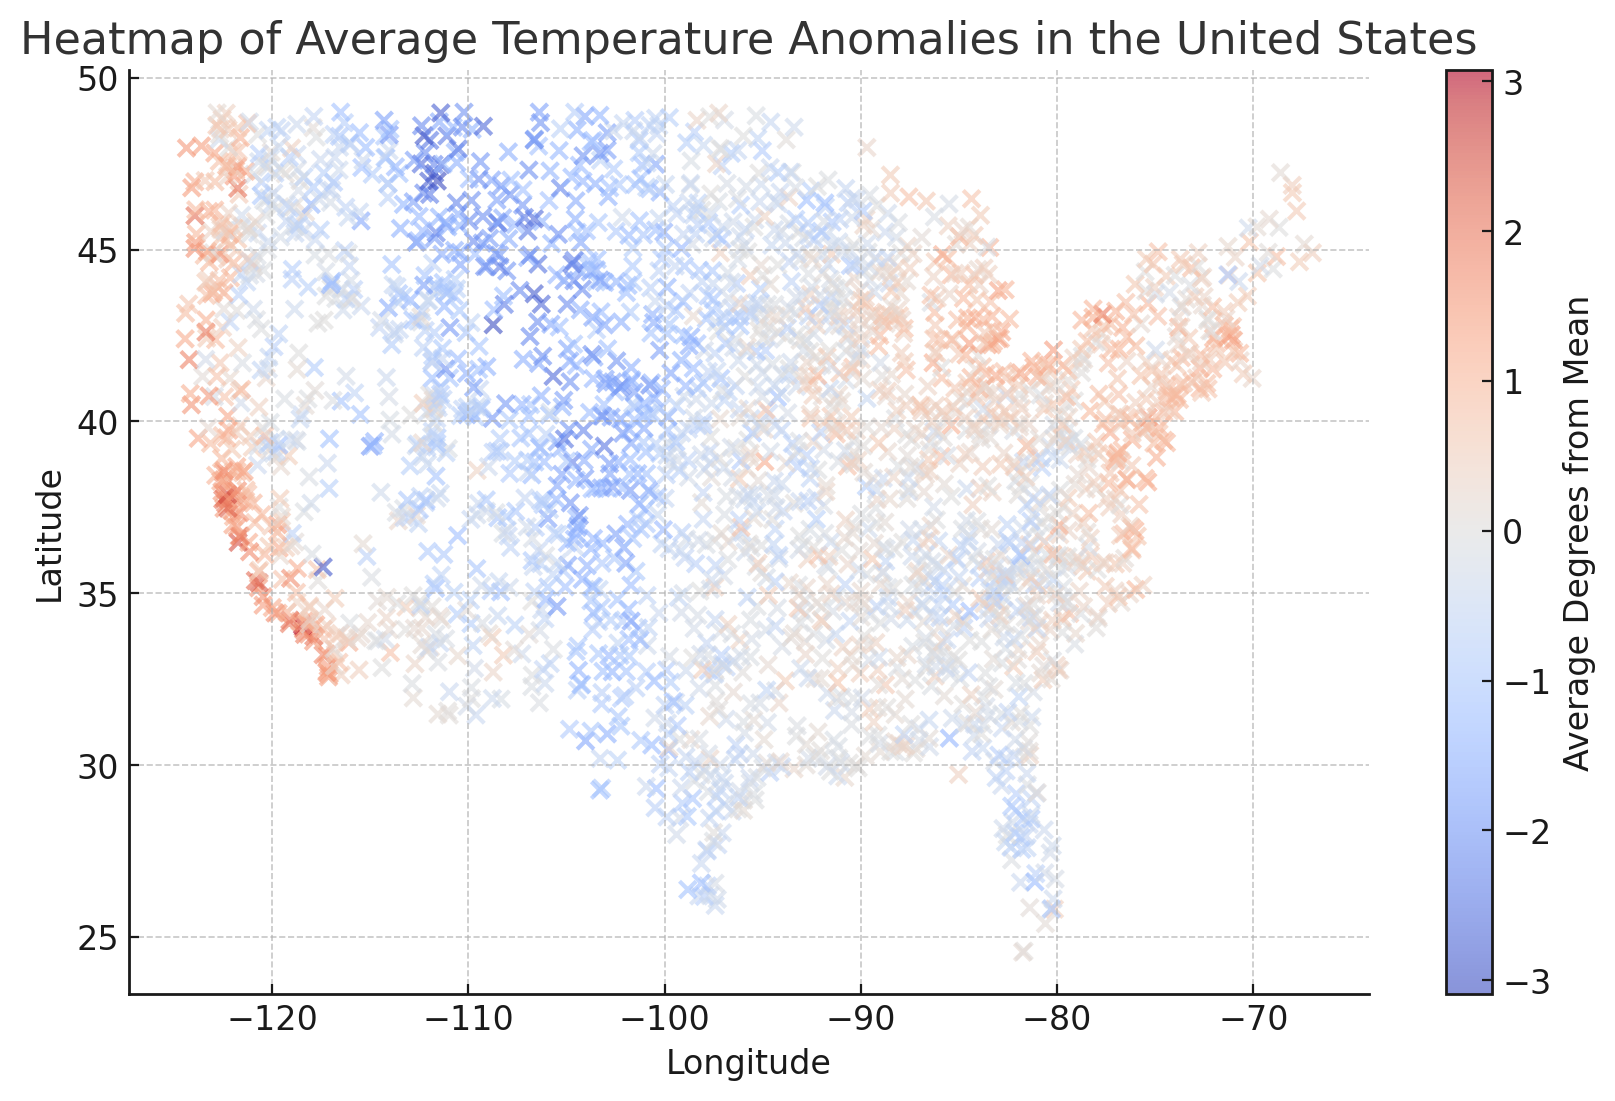
\includegraphics[width=\textwidth]{visuals/weather_visuals/Heat_map_USA.png}
\caption{Heatmap of Average Temperature Anomalies in the United States.}
\label{fig:heatmap_usa}
\end{figure}

This analysis has several aspects to it which make it challenging. The data spans extensive time periods and geographical area. These temporal and spatial structures must be handled appropriately. With data from numerous weather stations expanding rapidly over time, we limit our analysis to 1990 - 2010 data from 249 stations, selected one per 2x2 latitude/longitude grid, to manageably capture seasonal trends and geographical representation while staying within our available computational resources.

We applied a time series decomposition using base R tools, with a 365-day frequency to extract seasonal, trend, and residual components from the data. For the spatial dimension, we combined latitude and longitude information to define points for a K-nearest neighbors (KNN) algorithm, to determine spatial weights. These weights were used for generating a spatial lag variable to account for the spatial auto-correlation in temperature anomalies.

A visualization of the dataset reveals a bimodal distribution in the degrees from mean variable, which represents hot and cold anomalies. Our two-stage analytical approach consisted of:
\begin{itemize}
\item Employing a logistic regression classifier to distinguish between hot and cold anomalies.
\item Utilizing Gaussian models to quantify the extent of temperature deviations within each category.
\end{itemize}

\subsubsection{Model Selection - Classifier}

The classifier is designed to address both temporal and spatial autocorrelation, capturing the inherent dynamics and patterns in weather data to ensure accurate and context-sensitive predictions.

\begin{figure}[H]
\centering
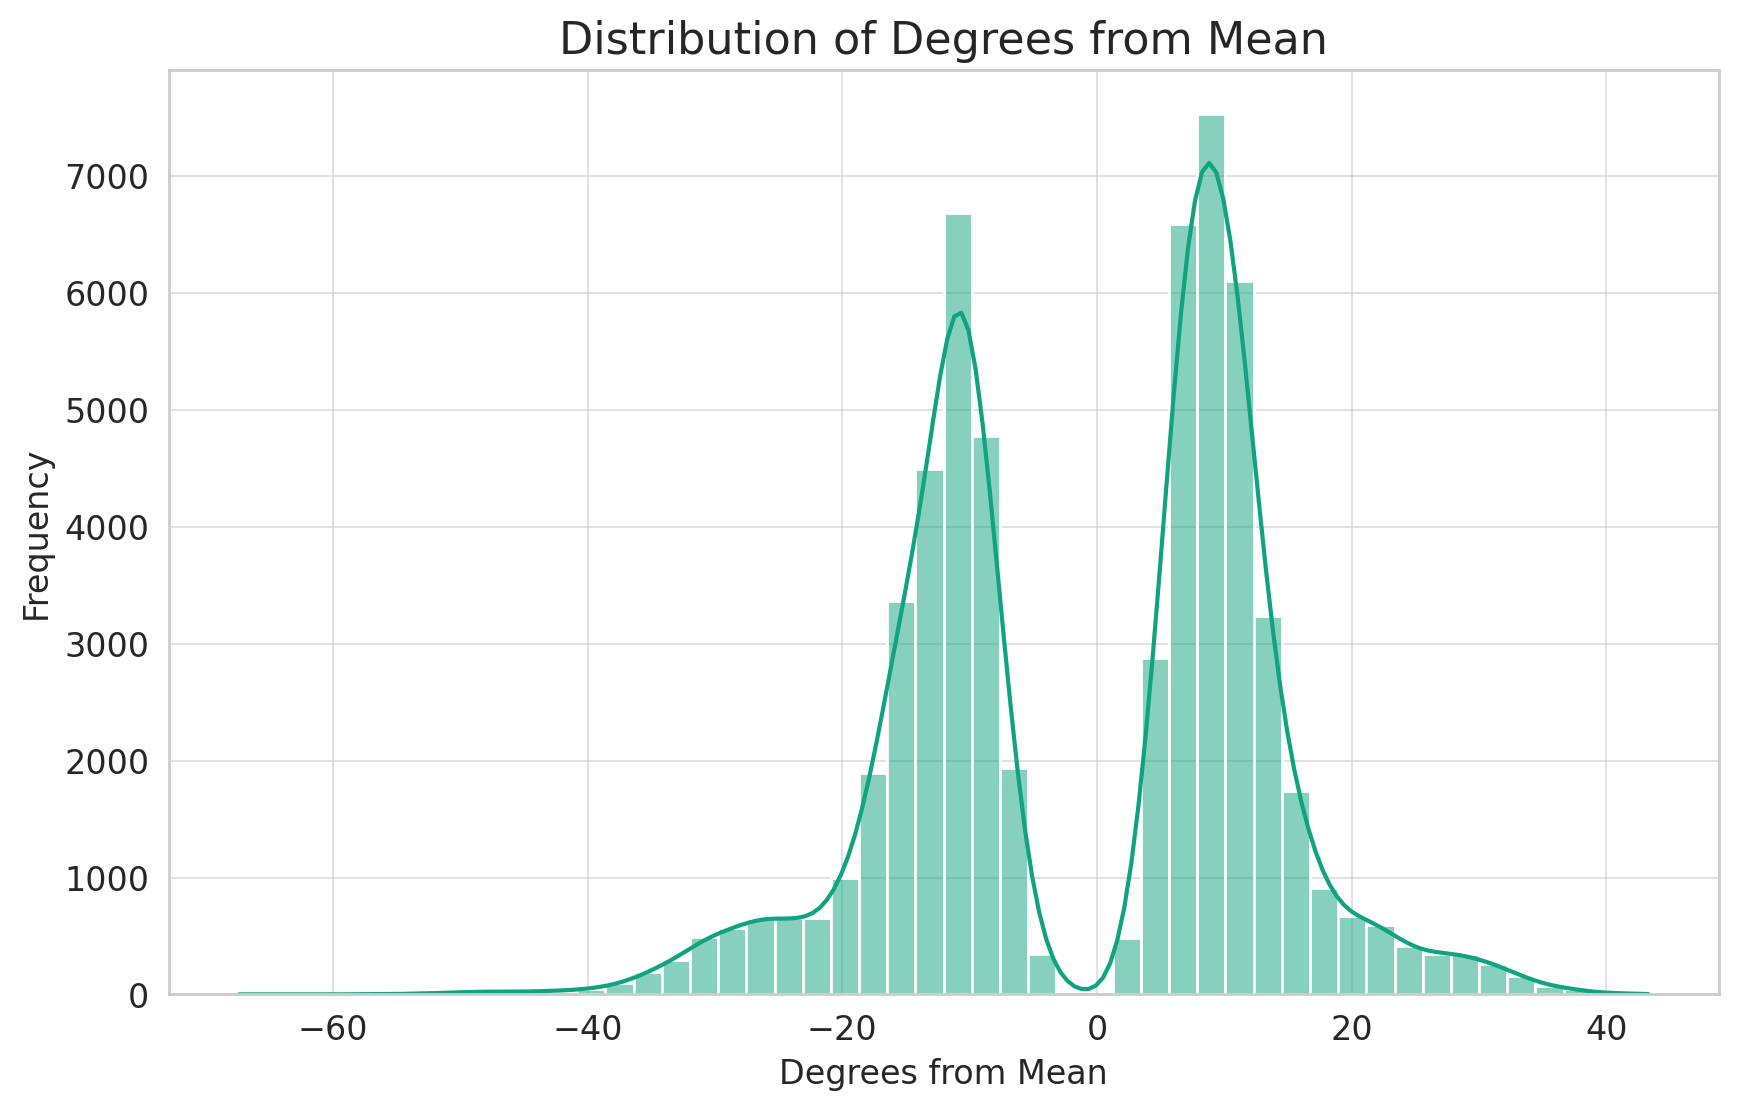
\includegraphics[width=\textwidth]{visuals/temperature_model_anomalies/degr_from_mean.png}
\caption{Bimodal distribution of the degrees from mean variable, suggesting two distinct normal distributions.}
\label{fig:deg_from_mean_dist}
\end{figure}

\begin{lstlisting}[language=R]
glmmTMB(hot_cold_indicator ~ s(time€ + (1|month€ +
                s(max_temp€*s(min_temp€ +
                s(latitude€ * s(longitude€ +
                s(trend€ + s(spatial_lag€ + 
                s(seasonal€,
                data = train_data,
                family = binomial(link="logit"€,
                REML = TRUE€
\end{lstlisting}

\subsubsection{Results}

A 5-fold cross-validation gave an average F1 score of 0.978. This score is higher than the test data score below, likely due to the final model having a several of the smooths specified with a reduced number of knots.

\begin{figure}[H]
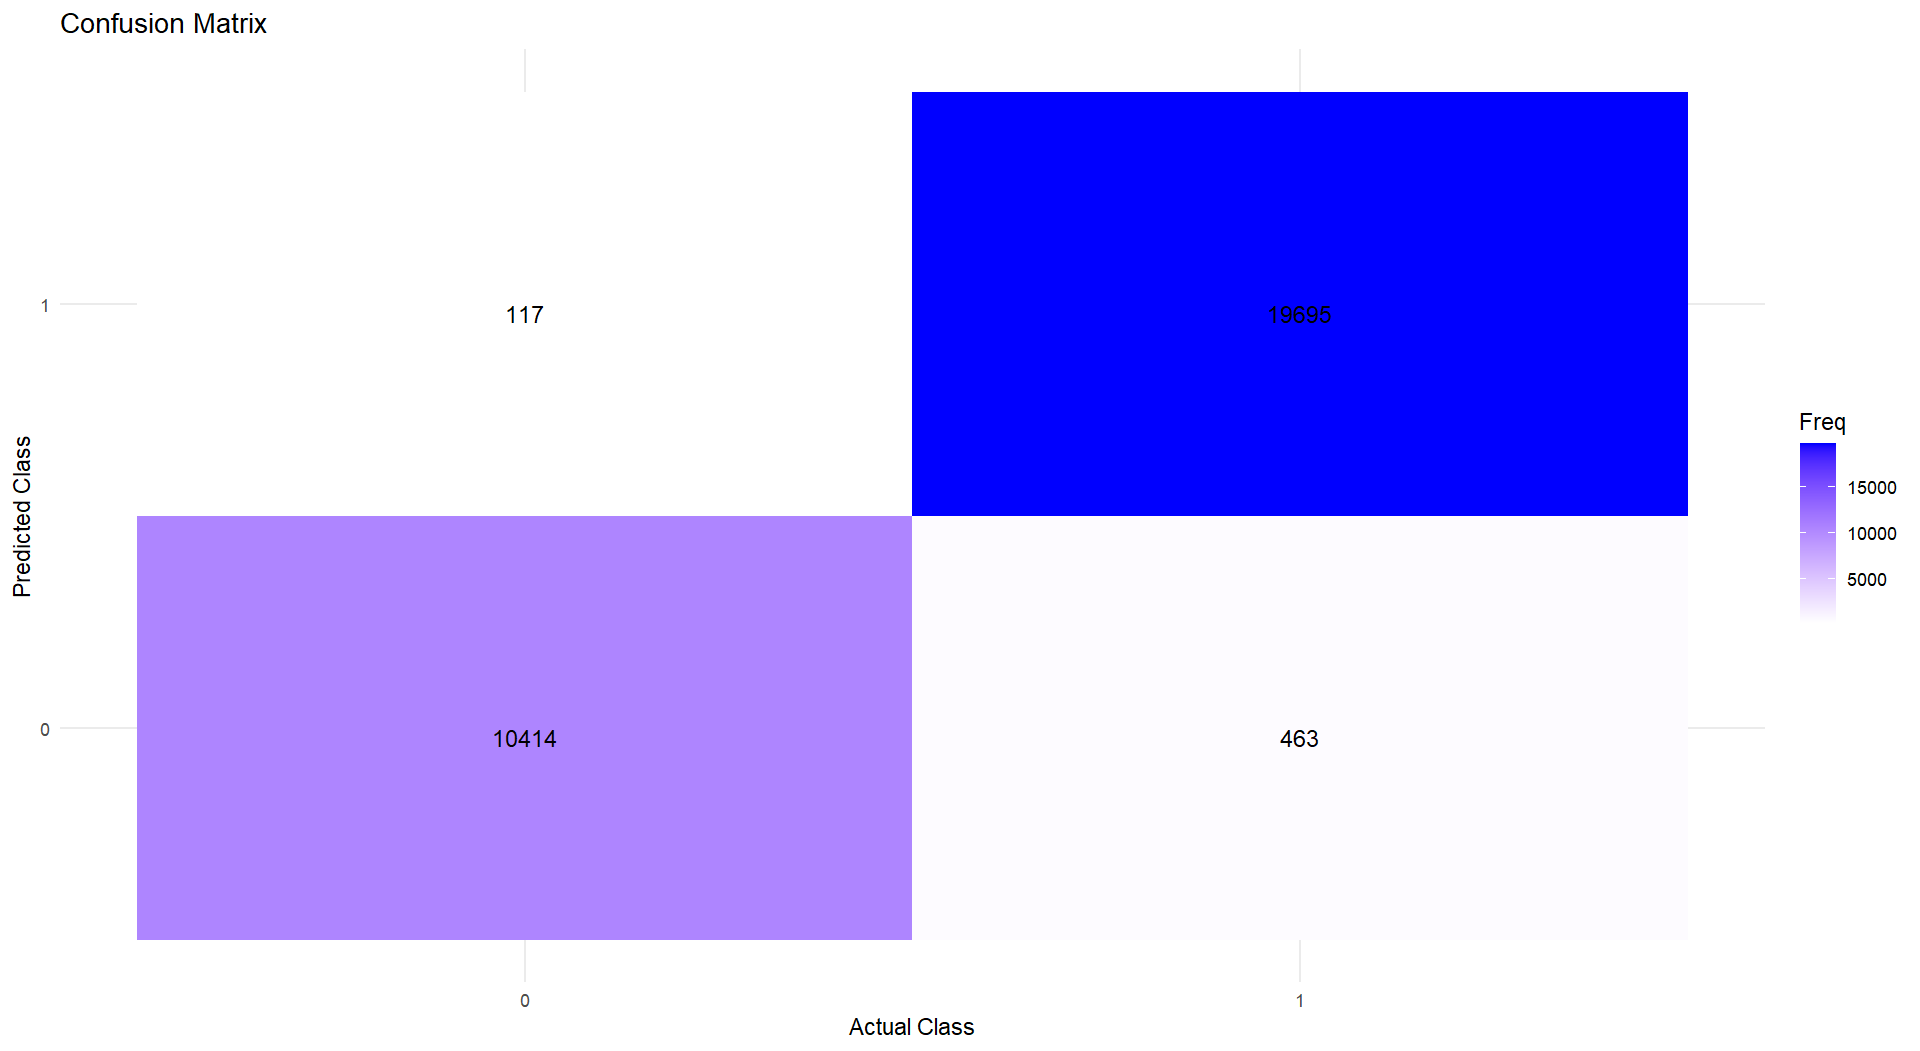
\includegraphics[width=\textwidth]{visuals/temperature_model_anomalies/final_cm.png}
\caption{Test Data Predictions Confusion Matrix demonstrating balanced accuracy, precision, and recall.}
\label{confusion_matrix}
\end{figure}

\begin{table}[H]
\centering
\begin{tabular}{lr}
\hline
Metric & Value \\
\hline
Accuracy & 0.981 \\
No Information Rate & 0.645 \\
Sensitivity (Recall) & 0.957 \\
Specificity & 0.994 \\
Precision (Pos Pred Value) & 0.989 \\
Neg Pred Value & 0.977 \\
Balanced Accuracy & 0.976 \\
F1 Score & 0.972 \\
\hline
\end{tabular}
\caption{Performance metrics of the classification model show high accuracy and balanced accuracy (0.977), confirming effective prediction for both anomaly categories. An F1 score of 0.972 underscores a robust balance between precision and recall. Significant improvement over a no-information rate of 0.645 and a Kappa score of 0.958 indicate the model's reliability and substantial predictive advantage.}
\label{table:performance_metrics}
\end{table}

Since we haven't used any capabilities here that aren't in the \texttt{gamm} toolbox, the results are essentially the same, and therefore we have omitted the performance metrics and plots from the \texttt{gamm} model.

\subsection{Temperature Anomalies: Gaussian Models}\label{sec:analysis:degrees_from_mean}

Our approach is to use two Gaussian models to separately address hot and cold temperature anomalies. This will make it easier to capture the bi-modal distribution, by modelling each mode separately. We can't think of any way to specify a a single regression model in these frameworks with the kind of mean-variance relationship of the degrees from mean data. Additionally, Gaussian models are usually efficient and robust to fit, and are less prone to convergence issues. 

\subsubsection{Model Selection}

We use the same approach as in the classifier to handle the spatial and temporal structures. The predictor set is largely similar for these models, but we now use the \texttt{type} variable to model the dispersion, which slightly enhanced our ability to more accurately model the tails of the distribution, although capturing their full extent remains challenging. 

\begin{lstlisting}[language=R]
glmmTMB(dfm ~ s(time€ + 
            s(max_temp€ * s(min_temp€ +
            s(longitude, latitude€ +
            s(trend€ + s(spatial_lag€,
            disp =~ type,
            family = gaussian(€,
            data = combined_data_hot,
            REML = TRUE€

glmmTMB(dfm ~ s(time€
            s(max_temp€ * s(min_temp€ +
            s(longitude, latitude€ +
            s(trend) + s(spatial_lag€,
            disp =~ type,
            family = gaussian(€,
            data = combined_data_cold,
            REML = TRUE€
\end{lstlisting}

\subsubsection{Results}

As we've already come to know, more training data really helps predictions for this data, as the seasonal aspects and longer term cyclical climate processes are likely quite important in accurately accounting for temperature deviations. Even at 20 years of data there is still some sensitivity (albeit much less) to specific characteristics of the validation and test sets. For instance the average RMSE for the combined models on an expanding windows cross validation was significantly lower (better) than on the test set.

\begin{table}[H]
\centering
\begin{tabular}{lr}
\hline
Model & RMSE \\
\hline
No Dispersion Adjustment & NA \\
Default Dispersion (1) & 3.03 \\
Dispersion Adjusted by Type & 2.64 \\
\hline
\end{tabular}
\caption{Test data performance: Adjusting the dispersion formula produced different outcomes, as one might expect. Setting dispersion to zero forces variance into the random effects, which is an interesting ability, but which in this case caused convergence issues. The best performance was achieved with the dispersion modelled by type.}
\label{table:performance_metrics}
\end{table}

\begin{figure}[H]
\centering

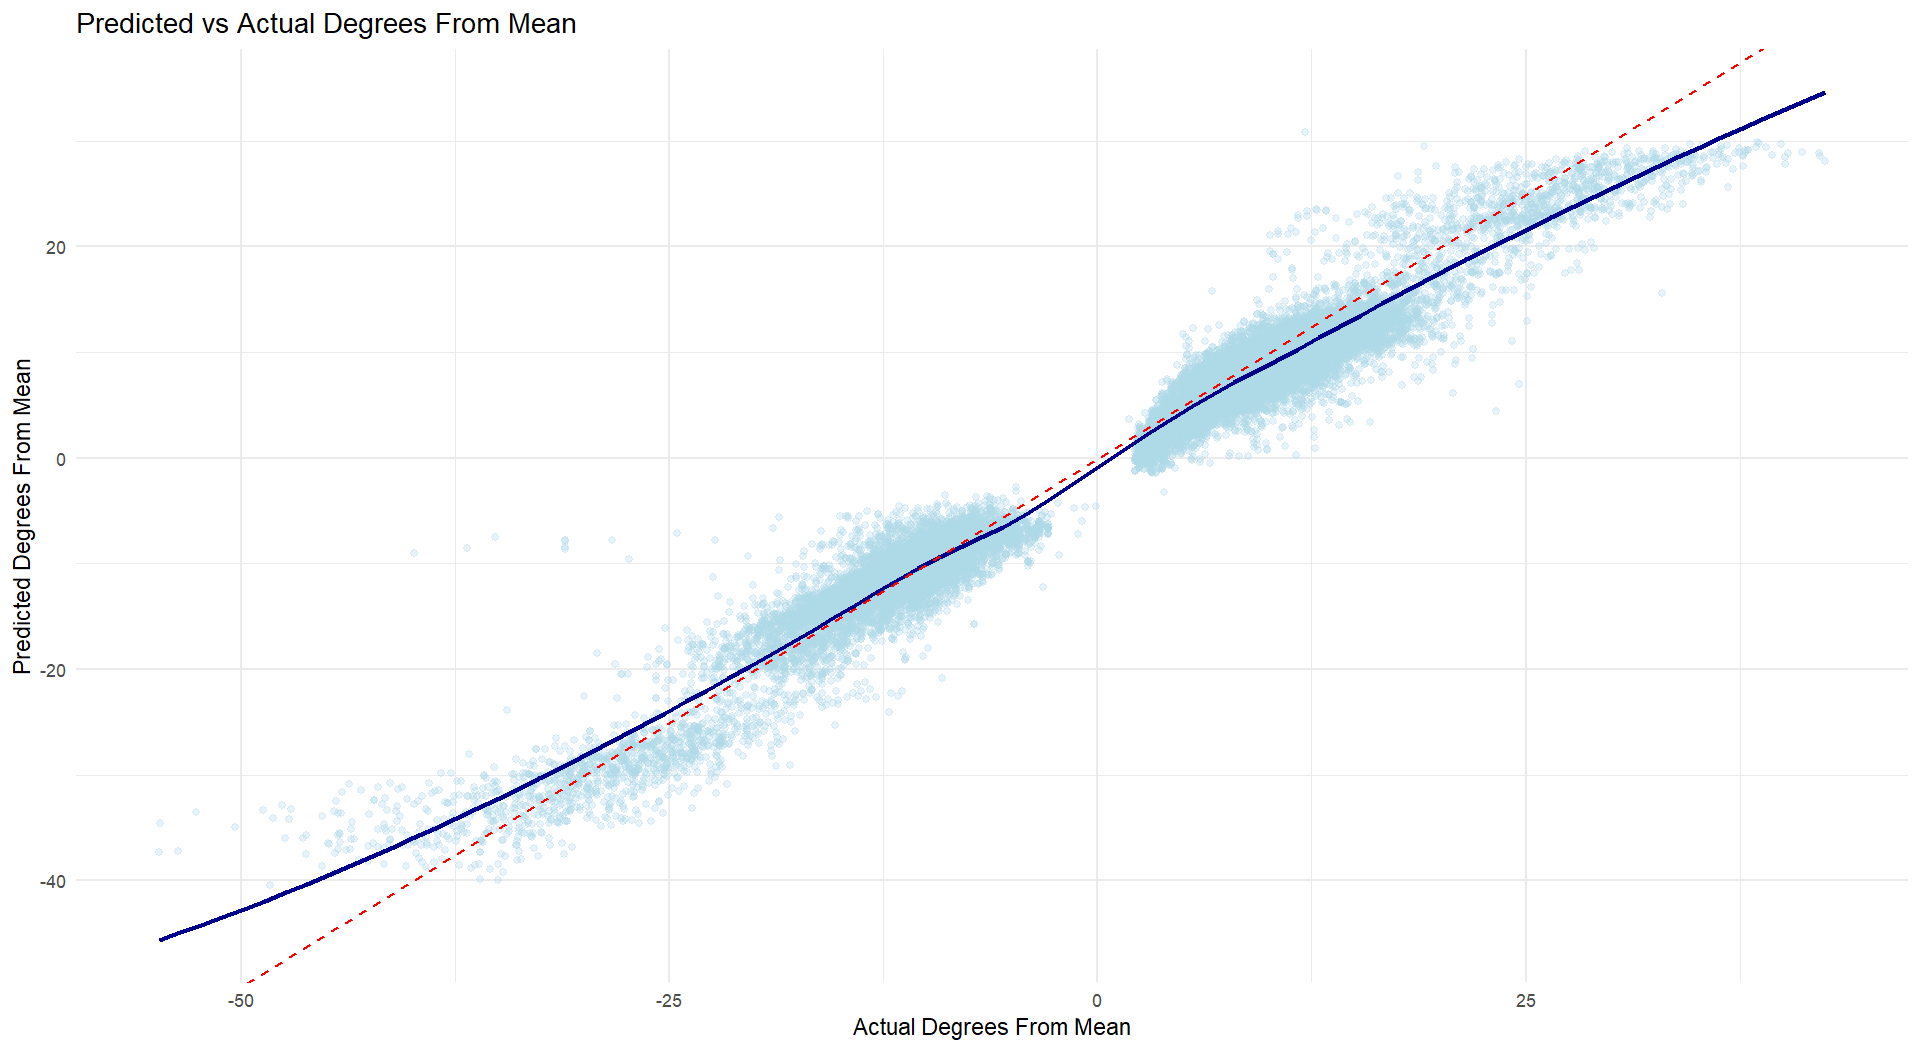
\includegraphics[width=\textwidth]{visuals/temperature_model_anomalies/final_loess_temp.png}
\caption*{Loess-smoothed plot comparing predicted versus actual values.}
\label{fig:hist_pred_errors}

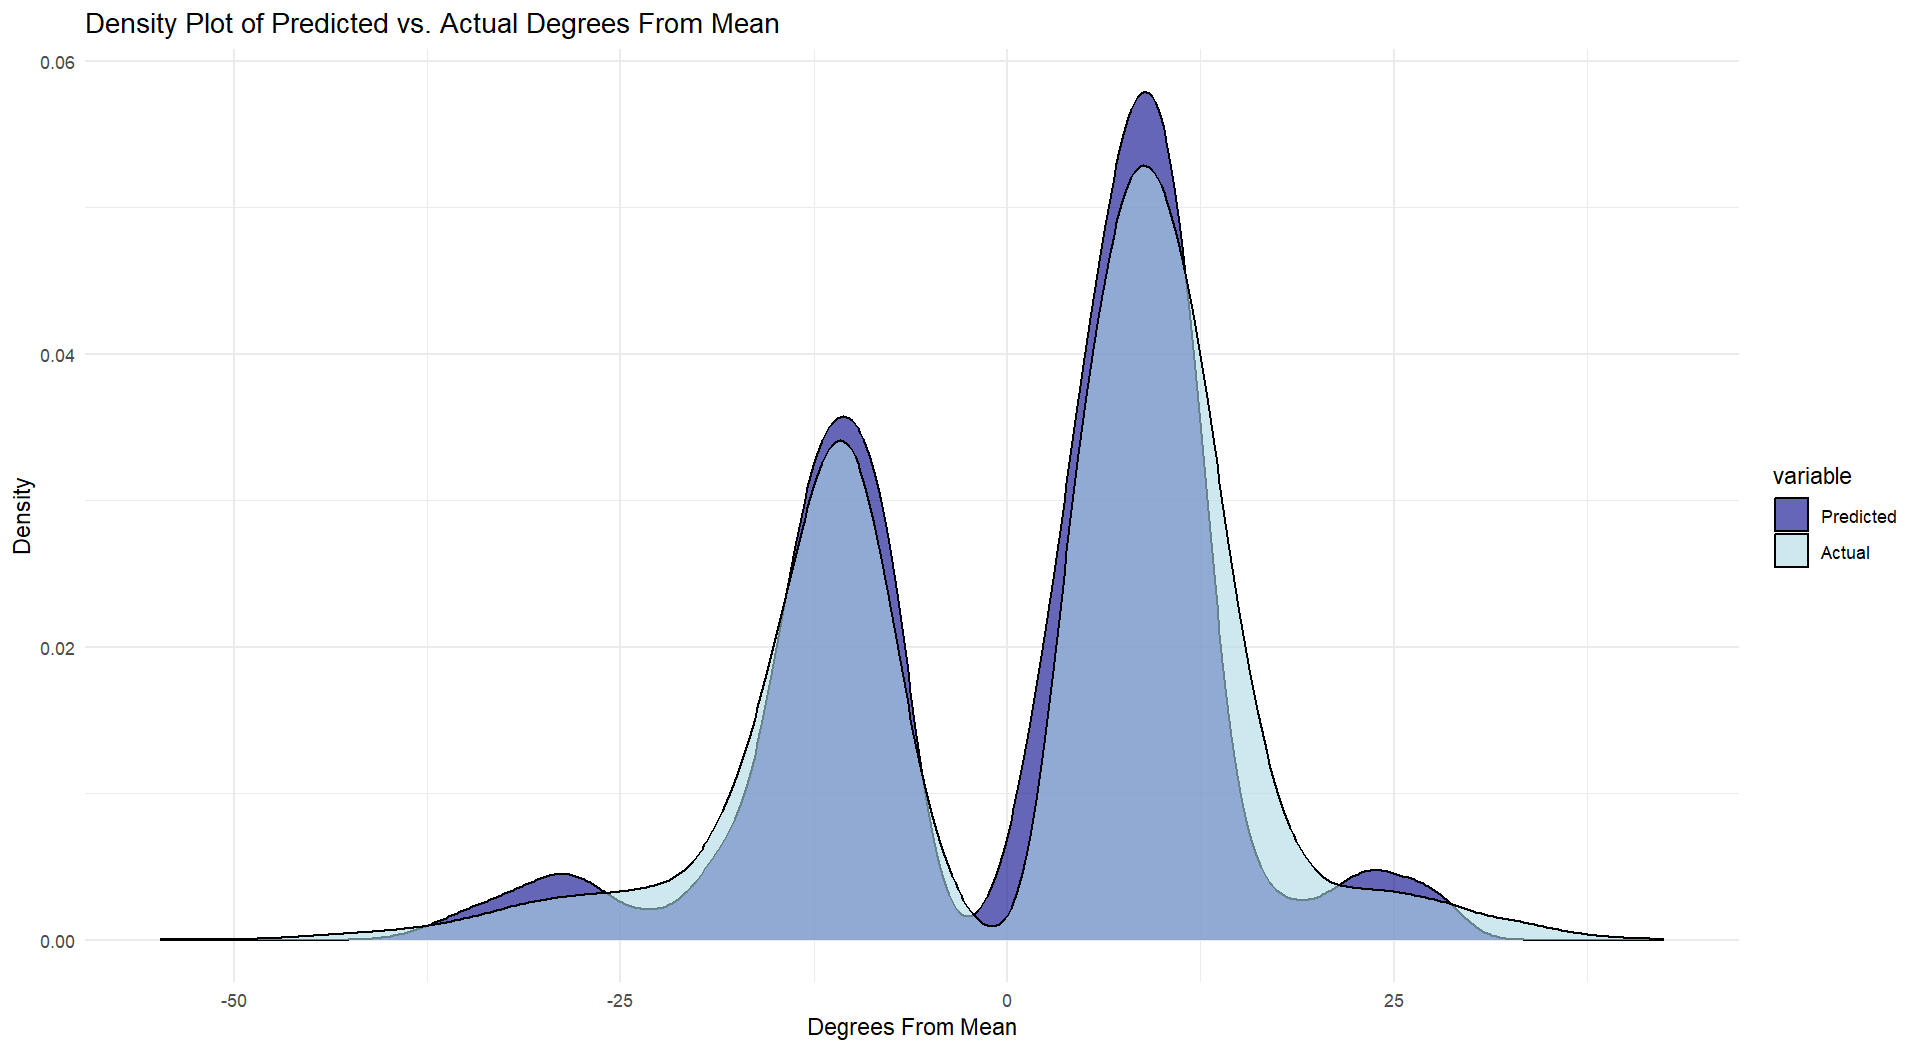
\includegraphics[width=\textwidth]{visuals/temperature_model_anomalies/final_density_temp.png}
\caption*{Density plot of predicted versus actual values.}
\label{fig:predicted_vs_actual_densities}

\caption{Performance on Test Data for Temperature: These visualizations highlight the models' effectiveness in capturing the core distribution while noting challenges with extreme values.}
\label{fig:test_data_performance_4}
\end{figure}

\subsection{Wind Speeds}\label{sec:analysis:windspeed}

This data set contains wind speeds and other meteorological parameters collected from 54 weather stations on the west coast of USA. The data goes back to 1981 and contains at the time of our download of the data observations up to 2023. The data originates from three sources: Santa Barbara County Air Pollution Control District, California Department of Water Resources, and National Data Buoy Center. The latter source provides water temperature observations. The dataset contains hourly observations.

To determine the most influential factors affecting wind speed (\texttt{spd}), we lagged variables, since we are dealing with time series data, and then used a Random Forest feature importance analysis and. The analysis identified key variables that significantly predict the response variable \texttt{spd} (wind speed). These variables include:

\begin{itemize}
    \item \textbf{spdlag:} The speed of the wind measured in meters per second one hour prior.
    \item \textbf{Time:} Continuous variable which takes value 1 at the first observation and increments by 1 for each subsequent observation.
    \item \textbf{Utau, Vtau:} Wind stress in U and V directions.
    \item \textbf{Abar:} Atmospheric pressure in mBar.
    \item \textbf{Atmp:} Air temperature in Celsius.
    \item \textbf{Wtmp:} Water temperature in Celsius.
\end{itemize}

\textbf{Note:} \texttt{spdlag} is the only variable explicitly named with the lag suffix, but all of the predictor variables are lagged (an equal amount). 

The calculation of wind stress (\(\tau\)) uses the formula \(\tau_o = C_D \cdot \rho \cdot V_{10}^2\), where \(C_D\) represents the drag coefficient, \(\rho\) denotes the air density, and \(V_{10}\) is the wind speed at a 10-meter altitude.
\newline

For the analysis, the dataset was filtered to include all observations from 2021. The models will predict/forecast the wind speed one hour forward in time. We will select out one weather station which has complete information (no NAs) for all variables and no missing observations. Weather station 46078 (Albatross Bank) fits into this category, so we'll choose it.

\subsubsection{Model Selection}

Our analysis of wind speeds will aim to investigate:

\begin{enumerate}
    \item If a GAM more accurately captures complex and non-linear physical phenomena like wind, compared to linear models. \\
    \item How flexibility in dispersion modelling can help with predicting extreme values of a distribution.
\end{enumerate}

We hypothesize that combination of $U_\tau$ and $V_\tau$ would be captured well by a bivariate TPRS spline smooth. These bivariate smoothers do however come at a significant computational cost.

\textbf{Note}: Parallelization and distributed methods can alleviate temporal burden, at the cost of memory overhead and increased hardware/compute cost.
\newline

The model and training set sizes are slightly altered between the 1 hour and 24 hour forecasting models. Specifically we use 3 months of training data for the 1 hour forecasting model, and 9 months for the 24 hour model. This might seem somewhat arbitrary, but the reason behind it is that the doing the 1 hour model results in very many iterations through cross validation loop. We use a 90-10 split training to validation for the 1 hour mode, and a 80-20 split for the 24 hour model. It's also reasonable to assume it takes more training data to achieve good predictions with a farther forecasting horizon.

\begin{lstlisting}[language=R]
lm(spd ~ time + spd_lag +
        abar + Atmp + Wtmp + Utau + Vtau,
        data = train_data€

glmmTMB(spd ~ s(time€ + s(spd_lag€ +
        s(Utau, Vtau) + Atmp + Wtmp + s(abar),
        disp =~ 1,
        data = train_data,
        family = gaussian€
\end{lstlisting}

\subsubsection{Results}
The results are slightly in favour of the GAM, with a RMSE score of 0.924 against 0.928 for the linear model.

\begin{figure}[ht]
    \centering
    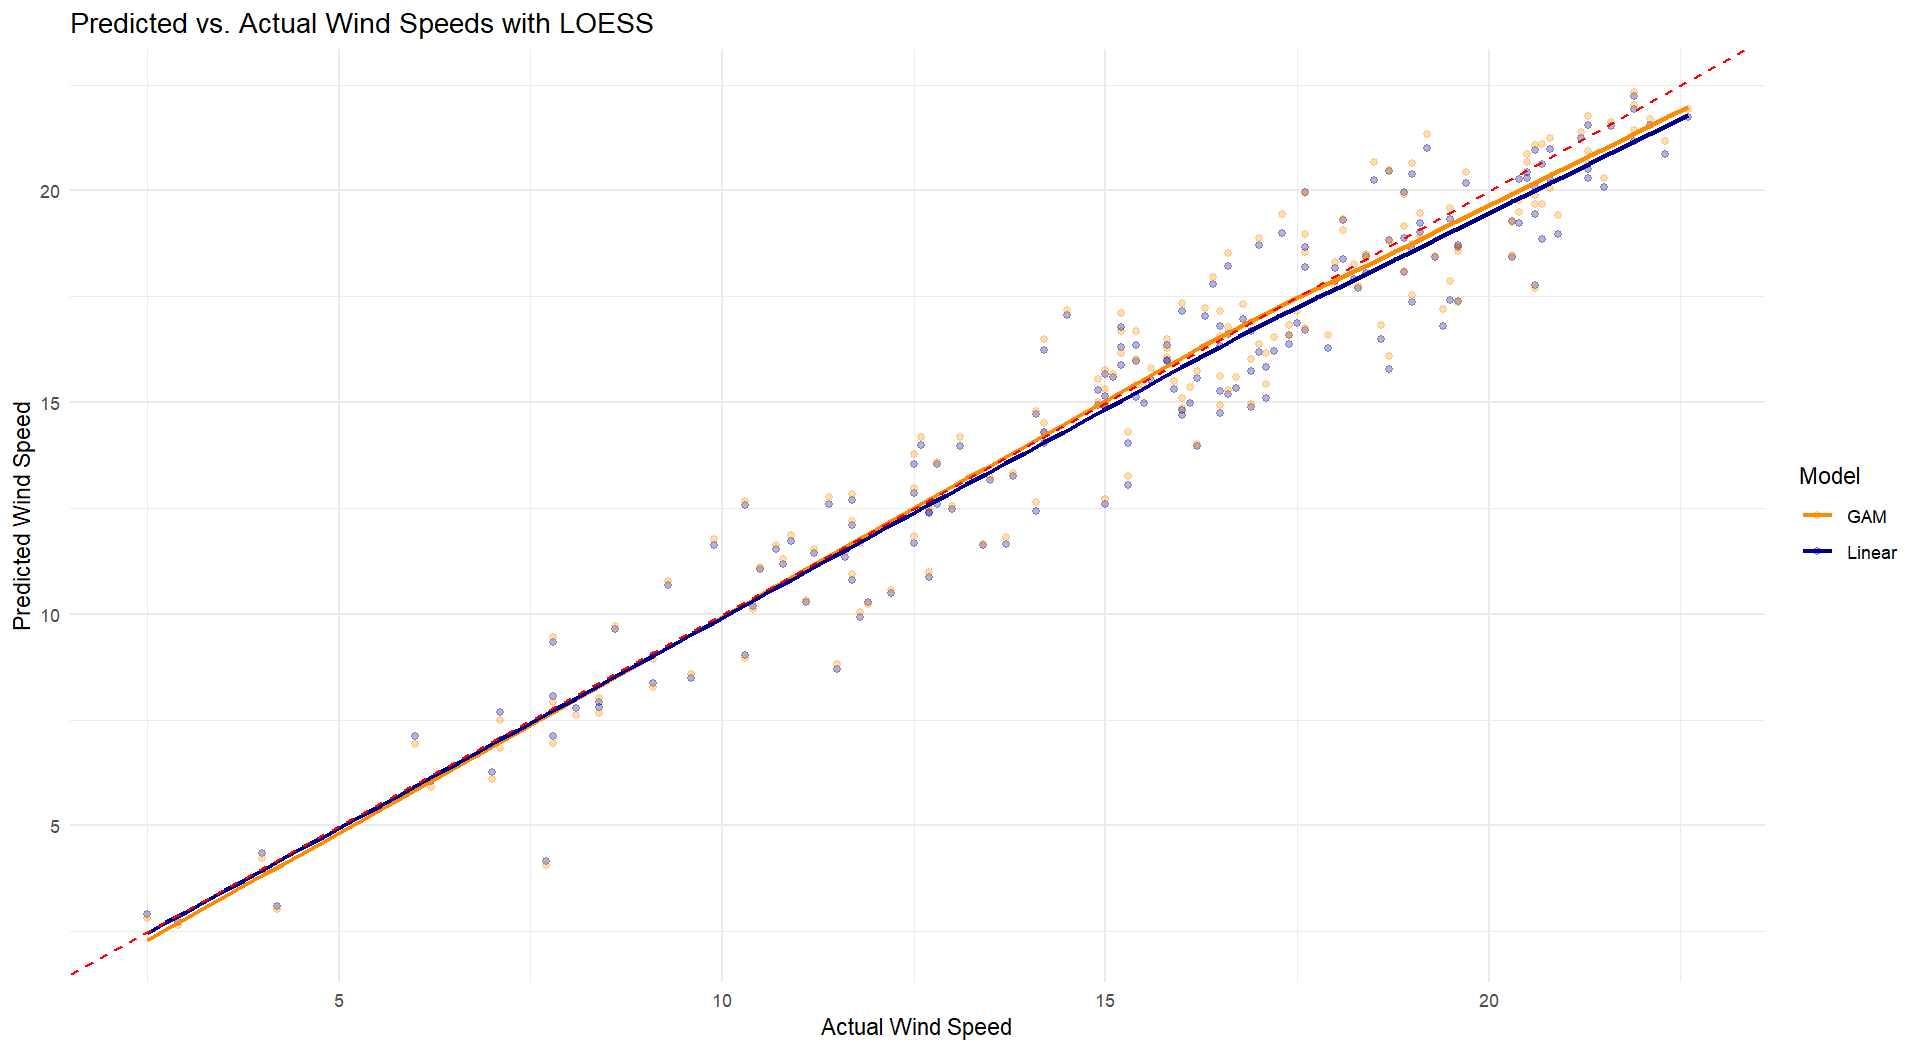
\includegraphics[width=\linewidth]{visuals/wind_model_speed/loess_wind_1.png}
    \caption{Loess regression line of predictions vs actual values for the 1 hour models.}
    \label{log_return_alt_rmse_folds}
\end{figure}

\begin{figure}[H]
    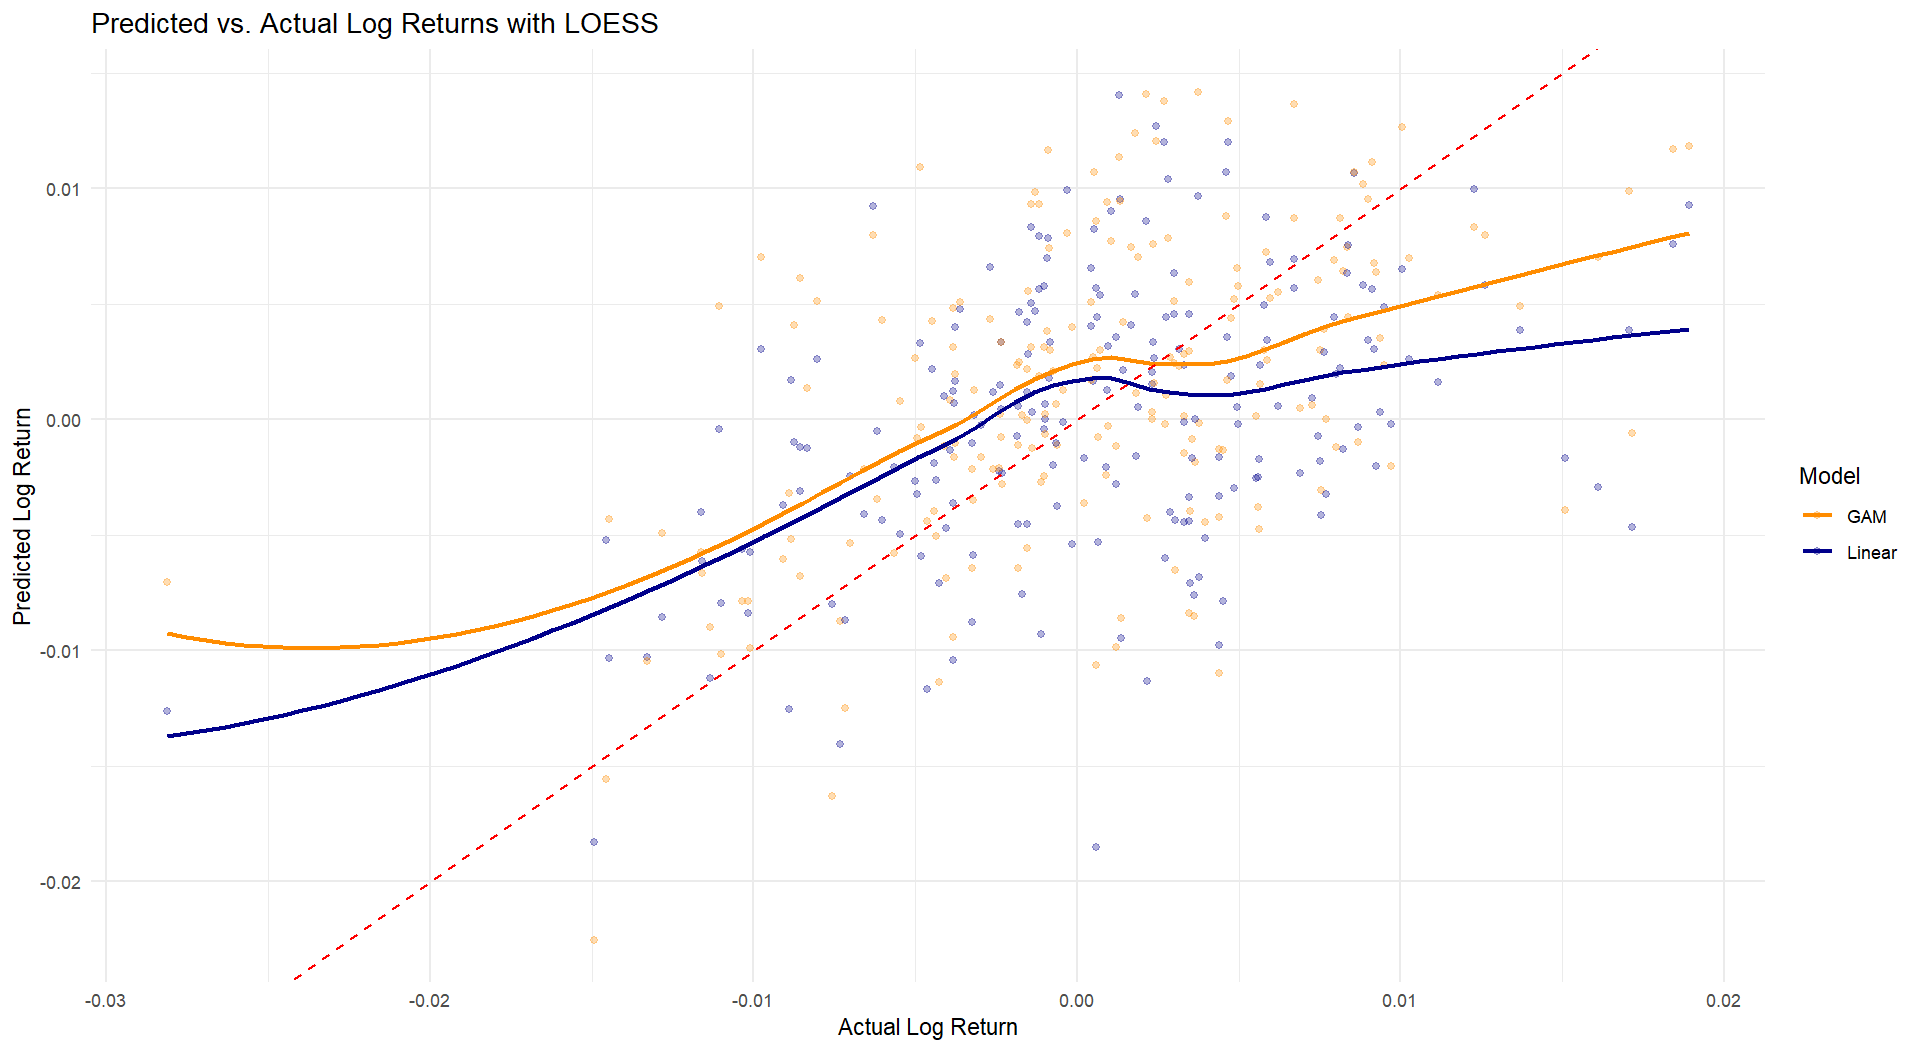
\includegraphics[width=\linewidth]{visuals/log_return/lr2_loess_bige_and_wide.png}
    \caption{Loess regression line of predictions vs actual values for the 24 hour models.}
    \label{log_return_alt_loess}
    \label{results:log_return_alt}
\end{figure}



\subsection{Wind Speeds II}\label{sec:analysis:storm_count}

Ideally, for this data set, we would create a sophisticated model capable of concurrent/global spatiotemporal predictions. However, that would be well beyond the scope of this paper. Instead we'll pick up where we left off above, see which improvements we can make on the first model, by including additional engineered variables and extending the forecasting horizon. For this analysis we'll compare \texttt{glmmTMB} against \texttt{gamm4} again, to investigate the benefit of a dispersion submodel for this data set. 

\subsubsection{Model Selection}

Based on the previous model, we select the following models. 

\begin{lstlisting}
gamm4(spd ~ s(time€ + spd_lag1 + 
            Atmp + R24 + abar,
            data = train_data,
            family = gaussian,
            REML = TRUE€
   
glmmTMB(spd ~ s(time€ + spd_lag1 + 
            Wtmp + Atmp + R24 + abar,
            disp =~ spd_lag2,
            data = train_data,
            family = gaussian, 
            REML = TRUE€
\end{lstlisting}

Here we've engineered a few new variables, including \texttt{R24} and \texttt{spd\_lag2} which represent a rolling 24 hour average, which we will include. 

\subsubsection{Results}

From the plots and the RMSE scores we see that the dispersion model helps the prediction accuracy by a little bit, enough that it's significant given how little effort it takes to include it. 

\begin{table}[H]
\centering
\begin{tabular}{lc}
\toprule
\textbf{Model} & \textbf{Average RMSE} \\
\midrule
gamm4 Model & 1.142982 \\
glmmTMB Model & 1.135019 \\
\bottomrule
\end{tabular}
\caption{Comparison of Average RMSE for gamm4 and glmmTMB Models}
\label{tab:average_rmse_comparison}
\end{table}

\begin{figure}
    \centering
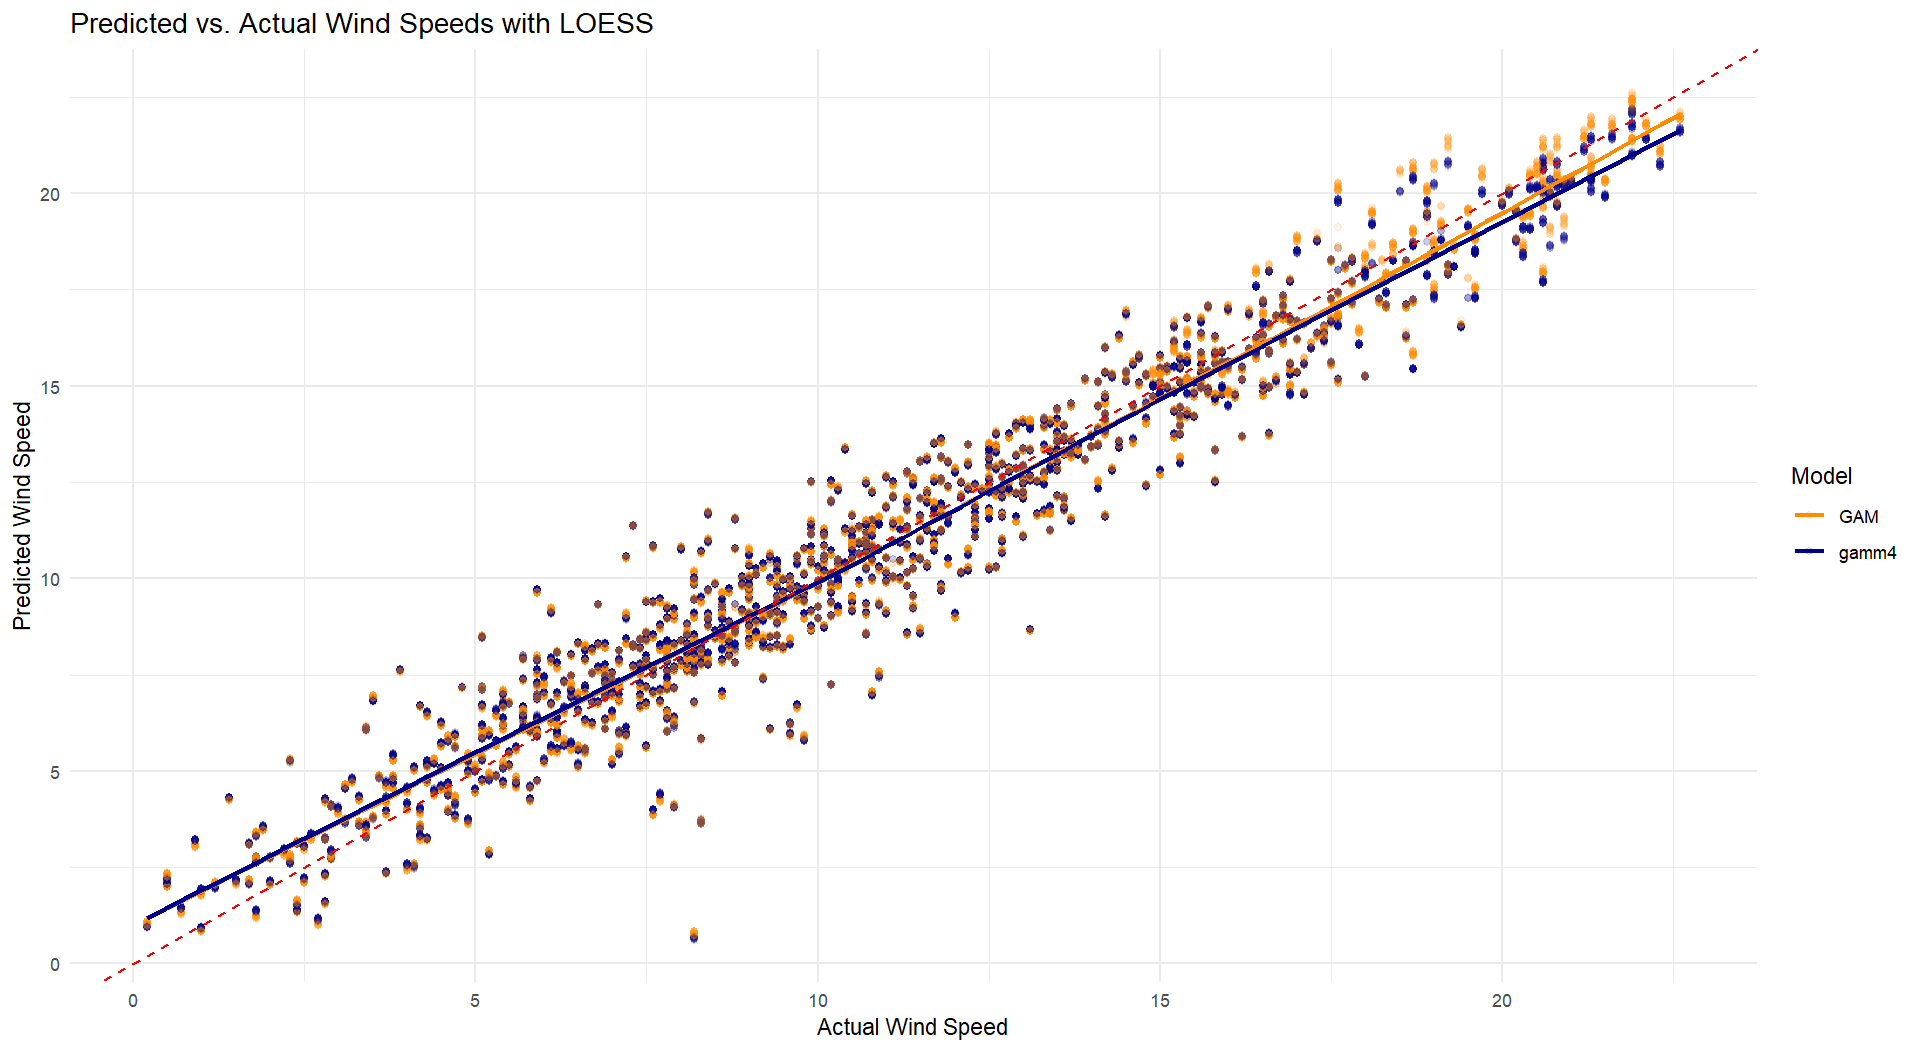
\includegraphics[width=0.8\textwidth]{visuals/wind_model_speed/loess_wind3.png}
\caption*{Loess-smoothed plot comparing predicted versus actual values.}
\label{fig:hist_pred_errors}
\end{figure}



\subsection{Claim Severity}\label{sec:analysis:claim_severity}

In the next two sections we will introduce the Swedish Motor Insurance dataset, which is a part of the \texttt{GLMsData} package. The dataset includes third-party motor insurance claims in Sweden for the year 1977. This dataset stands as a foundational resource for statistical analysis in actuarial science, specifically aimed towards understanding the risk factors influencing insurance claims within the Swedish motor insurance sector.
We chose this particular dataset as it is used in the original research of Tweedie distribution within insurance by \citet{JorgensenDeSouza1994}. 
\newline

The dataset is structured as a data frame containing 2182 observations across 7 variables. These variables offer a view of the claims process, incorporating aspects such as distance travelled, geographical zones, no-claim bonuses, vehicle make, number of insured policy-years, claims count, and total payment value in Swedish kroner, all described beneath;


\begin{itemize}
    \item \textbf{Kilometres:} Categorized into five levels, this variable signifies the annual distance covered by the insured vehicle.
    \item \textbf{Zone:} This denotes the geographical zone, ranging from urban centers like Stockholm to rural areas and Gotland.
    \item \textbf{Bonus:} Represents the no-claim bonus, quantified as the number of years plus one since the last claim.
    \item \textbf{Make:} Identifies the vehicle's make, with levels indicating common car models and a category for all other models.
    \item \textbf{Insured:} The count of insured policy-years.
    \item \textbf{Claims:} The number of claims filed.
    \item \textbf{Payment:} The total value of claims payments.
\end{itemize}

\subsubsection*{Claim Severity}

Claim severity refers to the average cost of claims over a period or for a certain category of claims. It is a measure used by insurance companies to understand the level of risk associated with insuring a particular group, policy, or coverage type.  As we do not have our own severity variable in our data set, we will refer to a proposal modeling our payment-variable using the claim counts as an offset function for modeling the claim severity.
\newline

While modeling the payment-variable gives good results using the Tweedie distribution, a severity variable would not model quite as good with the same distribution. It is also not normal including the zero counts when modeling severity. We therefore decided to make a classifier first for dividing the dataset into subsets where the claim count was zero or over zero, and model the severity afterwards using the subset containing non-zero counts.




\subsubsection{Model Selection}
The model being used as a classifier includes the number of insured as a spline, with a random effect on the zone variable;
\newline 

\begin{lstlisting}[language=R]
motorins$HasClaim <- 
    ifelse(motorins$Claims > 0, 1, 0€



classifier <- glmmTMB(HasClaim ~ s(Insured€+(1|Zone€,
                family = binomial(link = "logit"€,
                data = train_data€
\end{lstlisting}
The variables were chosen as they were significant and caused a lower AIC, considering our work on unseen data we also needed another performance metric. We therefore ran a confusion matrix for the model, with the two following tables showing our results. The accuracy of 91 percent gives a fairly decent result based on the two explanatory variables we have chosen.

\begin{table}[H]
\centering
\begin{tabular}{ccc}
\hline
\textbf{Prediction} \textbackslash \textbf{Reference} & \textbf{0} & \textbf{1} \\ \hline
\textbf{0} & 53 & 16 \\
\textbf{1} & 20 & 347 \\ \hline
\end{tabular}
\caption{Confusion Matrix for Claims}
\label{tab:confusion_matrix}
\end{table}


\begin{table}[H]
\centering
\begin{tabular}{@{}lr@{}}
\toprule
\textbf{Metric}            & \textbf{Value} \\ \midrule
Accuracy                   & 0.9174         \\
No Information Rate        & 0.8326         \\
Sensitivity                & 0.7260         \\
Specificity                & 0.9559         \\
Pos Pred Value             & 0.7681         \\
Neg Pred Value             & 0.9455         \\
Prevalence                 & 0.1674         \\
Detection Rate             & 0.1216         \\
Detection Prevalence       & 0.1583         \\
Balanced Accuracy          & 0.8410         \\ \bottomrule
\end{tabular}
\caption{Model Performance Metrics for the claim classifier}
\label{tab:logitregression:}
\end{table}

\newpage


Gamma and lognormal distribution are often used to model claim severity. However, the \texttt{mgcv}-package does not include the lognormal distribution, where as \texttt{glmmTMB} has it included as a family function.
We therefore tried the gamma distribution for the \texttt{gamm4}-model and the lognormal distribution for the \texttt{glmmTMB}-model, along with significantly tested explanatory variables. The lognormal distribution modelled well on seen data but did not work well during testing on unseen data. We therefore concluded with using the gamma distribution for both models.
\newline

We used the insured-variable as a spline also in this model, with bonus as an additional explanatory variable. To show the flexibility with the \texttt{glmmTMB}-package we also tried implementing variables in the dispersion sub-model. Adding the kilometres-variable as a dispersion parameter showed some improvements.
\newline

Using the proposition from \citet{tiwari2020modeling} our main takeaway is using counts as an offset. This is presented by generalized linear model theory.


\noindent
The generalized linear model (GLM) is set up as follows:
\begin{equation}
    \frac{\text{Claim cost}}{\text{Claim count}} = \exp(f(X))
\end{equation}\label{offsetfunction}

\noindent
When taking natural logarithms on both sides, we get:
    \[ \log\left(\frac{\text{Claim cost}}{\text{Claim count}}\right) = f(X) \]


\noindent
Where ``$\log$'' is the link function and $f(X)$ is a linear combination of the selected predictive variables, the logarithms can be expanded as:
\[ \log(\text{Claim cost}) - \log(\text{Claim count}) = f(X) \]

\noindent
This can be further simplified by isolating the claim cost on one side, resulting in the final form which includes the offset term:
    \[\log(\text{Claim cost}) = f(X) + \log(\text{Claim count})\]

\noindent
Using the amount of claims as an offset gives us the following models;





\begin{lstlisting}[language=R]

full_model_glmmTMB <- glmmTMB(Payment~
                s(Insured€+Bonus+
                offset(log(Claims€€,
                disp=~Kilometres,
                family = Gamma(link="log"€, 
                data = full_train_data€

full_model_gamm <-gamm4(Payment~
                s(Insured€+Bonus+
                offset(log(Claims€€,
                family = Gamma(link="log"€, 
                data = full_train_data€

\end{lstlisting}

\subsubsection{Results}

\begin{table}[H]
\centering
\caption{Model Evaluation Results}
\label{table:model_evaluationmort}
\begin{tabular}{lcc}
\hline
\textbf{Model} & \textbf{Cross Validation RMSE} & \textbf{Test Data RMSE} \\
\hline
gamm4 & 125504.9   & 114604.3\\
glmmTMB & 124278.5 & 107440.1 \\
\hline
\end{tabular}
\end{table}

\begin{figure}[H]
\centering

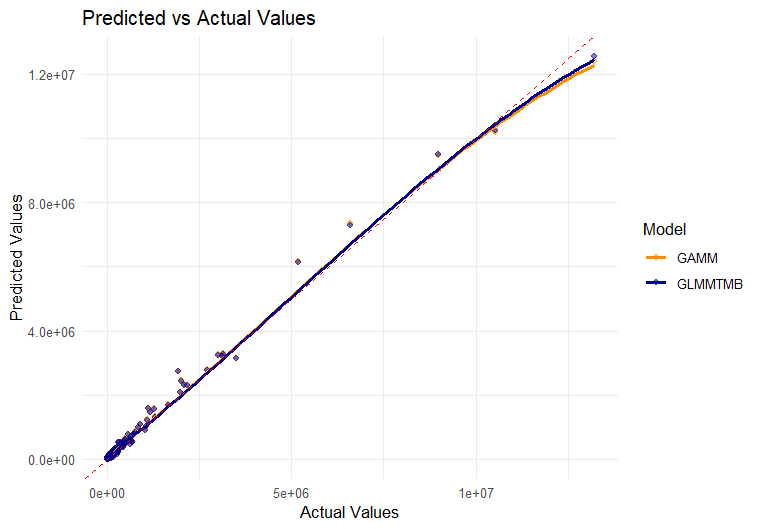
\includegraphics[width=0.8\textwidth]{visuals/InsuranceData/ClaimSeveritypredvact.png}
\caption*{Loess-smoothed plot comparing predicted versus actual values.}
\label{fig:hist_pred_errors}

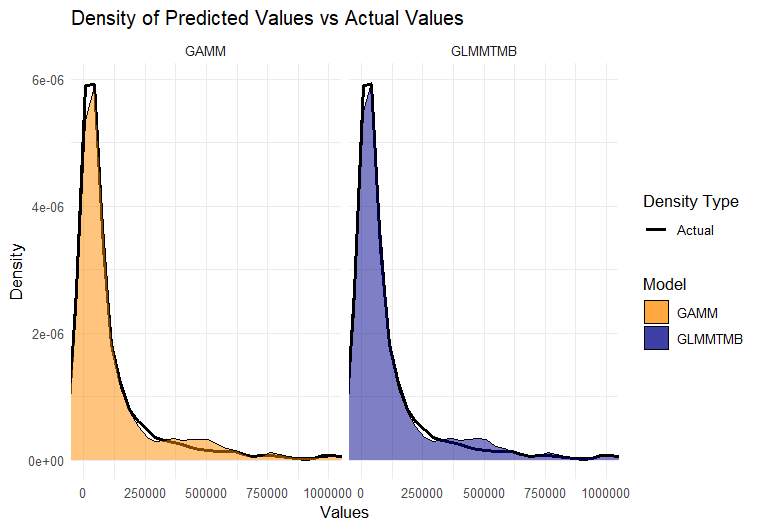
\includegraphics[width=0.8\textwidth]{visuals/InsuranceData/ClaimSeveritypredvactdens.png}
\caption*{Predicted vs Actual Densities. Scaled down for visualization purposes.}
\label{fig:predicted_vs_actual_densities}

\caption{Test data Performance for Claim Severity}
\label{fig:test_data_performance_4}
\end{figure}

From these visuals we can see that both models have rather 
good performance on unseen data. The RMSE, being rather large given the high values of payment values, but both are less than the mean of the values, meaning the model could be seen as fairly good. We see that the difference in predictions is as the values get higher, reflecting the dispersion parameter we have added to the \texttt{glmmTMB}-model.

\newpage

\subsection{Claim Counts}\label{sec:analysis:claim_counts}
We will also use the same data set to model claim counts or claim frequency in insurance.
Predicting claim frequency is important for insurers to manage risks effectively, ensuring financial stability with enough reserve setting, and tailor pricing strategies accurately. It facilitates customer segmentation, aiding in the development of customized insurance products and ensuring competitive pricing. Accurate predictions will help insurers comply with regulatory requirements, maintaining solvency and industry standing. Essentially, it supports the operational and strategic decisions of insurance companies, enhancing their ability to serve customers while managing their risk exposure efficiently. As actuarial students both claim frequency and claim severity are important variables to be able to model.


\subsubsection{Model Selection}
Using an already well known data set meant that we had access to the R-documentation linked with the data found in \ref{sec:analysis:datasets}. Here it was said that the number of claims had a Poisson distribution, however, we thought it could be appropriate to model the claims with the Tweedie distribution instead, as the data seemingly could follow such a distribution as well as the Poisson. Testing with both Poisson and Negative Binomial distribution, both with and without zero-inflation, they did neither have better AIC nor RMSE compared to the model using the Tweedie distribution. 
This might be because of the large values of counts we are modeling, as the distribution is right-skewed and have heavy tails. The Poisson distribution does not account for much skewness under the assumption that mean should be equal to the variance. The Negative Binomial distribution should work better for this type of scenario, but in our case we have a very large range. Most data sets with claim counts has probably a range from one to ten, whilst our variable has many observations ranging all the way to 3000 because of large groupings. This range makes us think we can treat the variable as continuous, having a gamma distribution for the non-zero positive values, and therefore modeling the variable with the Tweedie distribution. 
\newline

For our research with claim counts we thought of the continuous variable Insured as a spline covariate. After researching we also found Bonus to be a significant explanatory variable, and using Zone as a random effect also provided better results. Running the following code gives fairly equal models, but not quite identical, which may have something to do round-off induced discrepancy in the power constant $\xi$.

\begin{lstlisting}[language=R]
glmmTMB_model<-glmmTMB(Claims~s(Insured€+Bonus
                +(1|Zone€,
                data=motorins,
                family = tweedie(€€

xi<-family_params(glmmTMB_model€


gamm4_model<- gamm4(Claims~s(Insured€+Bonus,
                random=~(1|Zone€,
                data=motorins,
                family = Tweedie(p=xi€€
\end{lstlisting}

Looking into the additional functions that can be provided with \texttt{glmmTMB} we saw an improvement adding the number of kilometres travelled to the dispersion formula. Our final model would then look like this;

\begin{lstlisting}[language=R]
glmmTMB_model<-glmmTMB(Claims~s(Insured€+Bonus
                +(1|Zone€,
                disp=~Kilometres,
                data=motorins,
                family = tweedie(€€
\end{lstlisting}

\subsubsection{Results}


\begin{table}[H]
\centering
\caption{Model Evaluation Results}
\label{table:model_evaluationmort}
\begin{tabular}{lcc}
\hline
\textbf{Model} & \textbf{Cross Validation RMSE} & \textbf{Test Data RMSE} \\
\hline
gamm4 & 76.69  & 102.77 \\
glmmTMB & 60.78 &  72.55 \\
\hline
\end{tabular}
\end{table}

\begin{figure}[H]
\centering

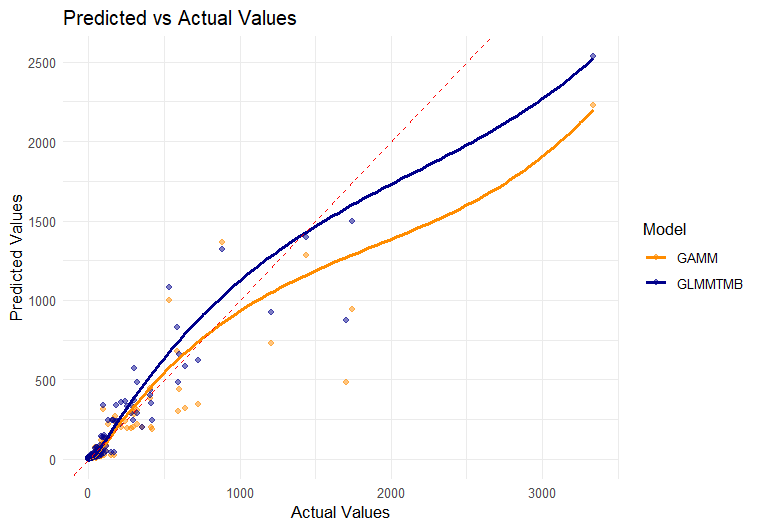
\includegraphics[width=0.8\textwidth]{visuals/InsuranceData/ClaimCountpredvact.png}
\caption*{Loess-smoothed plot comparing predicted versus actual values.}
\label{fig:hist_pred_errors}

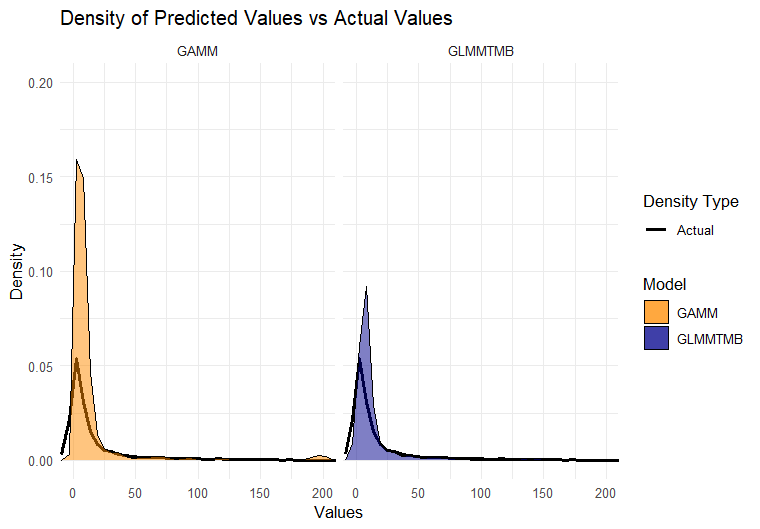
\includegraphics[width=0.8\textwidth]{visuals/InsuranceData/ClaimCountpredvactdens.png}
\caption*{Predicted vs Actual Densities. Scaled down for visualization purposes.}
\label{fig:predicted_vs_actual_densities}

\caption{Test data Performance for Claim Counts}
\label{fig:test_data_performance_4}
\end{figure}


From the performance on test data we can see that the there are a lot of zeroes to be accounted for in our modeling. Both models predict these values fairly similar, but as the value increases, the \texttt{glmmTMB}-model`s prediction is quite significantly better. Using Kilometres as a dispersion parameter seems to have made the model a better fit for the higher values and therefore has decreased the RMSE. Scaling the density plot to 200 counts gives us a better visualization on the lower values, where the \texttt{glmmTMB} model handles the prediction pretty well compared to \texttt{gamm4}.



\subsection{Face Value of Insurance Policies}\label{sec:analysis:face_value}

The \textit{ustermlife} dataset is sourced from the Survey of Consumer Finances (SCF), representing a nationally representative sample of U.S. households. It includes data from 500 households with positive incomes, surveyed in the year 2004. In this section we will try to model the Face value that was payed to customers within the period, however, we found it difficult to get a proper model using splines for these variables. Later we will try to interpret the Ridge penalty instead in search for improvements.
\newline

The variables in the dataset included Gender, Age, Education level and income to name a few. We tested different models with the continuous variables in splines, intuitively the Income and Age variables. Due to the extreme values of both the Face values and Income variables we also tried different methods of scaling and outlier-detecting to improve our models without much success. The thought of using logistic regression to predict and split the dataset into zero values and positive values for the Face variable also crossed our mind, but for this dataset we were determined to make the best model using the Tweedie distribution. 
We have pre-processed the data set and excluded the largest Face values, setting a maximum value at 500 000. Recall from \ref{nofreelunch} that by the no free lunch theorem, the performance of the model is contingent on the underlying assumptions being sufficiently met, so although the model performs well over a certain range of values, it may fail to do so completely outside of this range. Here the very large values would need a separate model, or a different approach altogether. There may be other factors to explain very large values which are discernible from the available data. The NFL theorem is not an excuse for a model not performing well, it simply implies that in order to obtain a strong model, one might need to explore many different approaches and models, and not expect one particular method to always work best for any given task. Often poor models are simply the result of poor data quality, or insufficient sample size for high-variance outcomes. 




\subsubsection{Model Selection}
For the model selection we tried multiple parameters as explanatory variables. Education was probably the most significant predictor when modeling face value, however, when using the variable along with splines on income and age we encountered convergence issues and decided to not keep Education for our research. 

Furthermore, we found the better model using a log-version of Income and Total Income as spline variables. The inclusion of Total Income did not have much effect, but to illustrate our Ridge model later in the thesis we chose to include both of the variables. We encountered convergence issues in this model as well in the \texttt{glmmTMB}-model, with no help of using start parameters we chose to include gender as a random effect which seemingly fixed our problem making the model run smoothly.


\begin{lstlisting}[language=R]

gamm4(Face~s(Income_log€
            +s(TotIncome_log€,
            family=Tweedie(p=xi€, 
            data = full_train_data€
                         

glmmTMB(Face~s(Income_log€+s(TotIncome_log€
            +(1|Gender€,
            family =  tweedie(€, 
            data = full_train_data€

\end{lstlisting}

\subsubsection{Results}

\begin{table}[H]
\centering
\caption{Model Evaluation Results}
\label{table:model_evaluationmort}
\begin{tabular}{lcc}
\hline
\textbf{Model} & \textbf{Cross Validation RMSE} & \textbf{Test Data RMSE} \\
\hline
gamm4 & NA  & 77423.05 \\
glmmTMB & NA &  79053.56 \\
\hline
\end{tabular}
\end{table}

\begin{figure}[H]
\centering

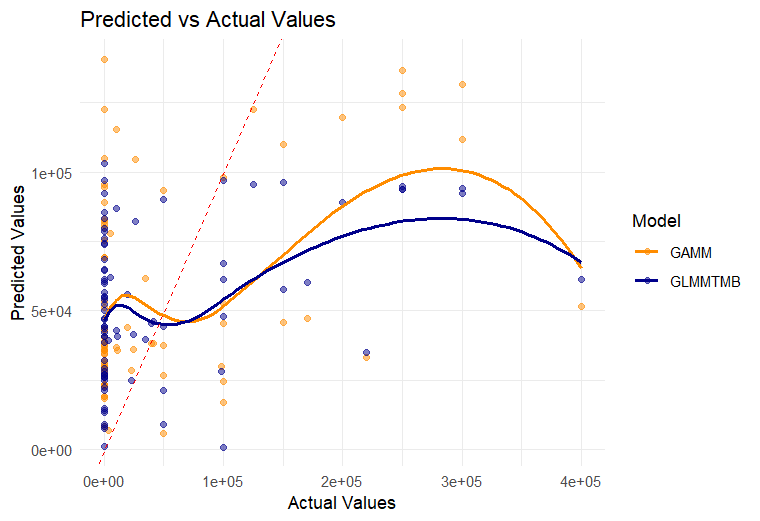
\includegraphics[width=0.8\textwidth]{visuals/InsuranceData/Facepredvact.png}
\caption*{Loess-smoothed plot comparing predicted versus actual values.}
\label{fig:hist_pred_errors}

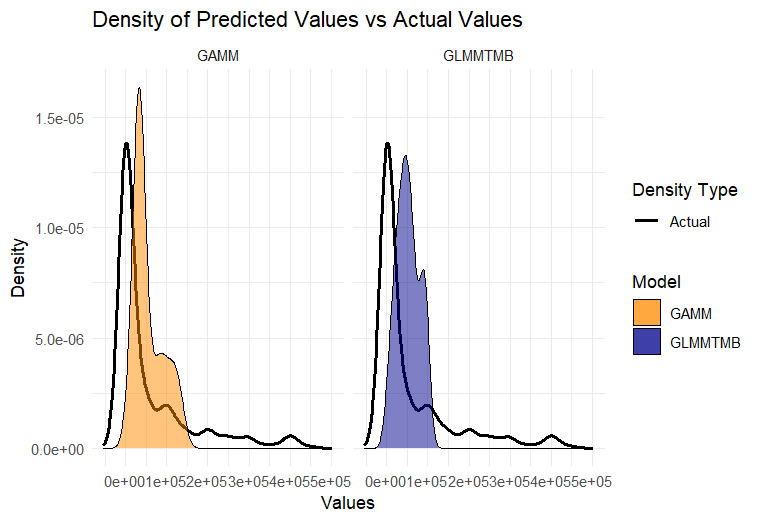
\includegraphics[width=0.8\textwidth]{visuals/InsuranceData/Facepredvactdens.png}
\caption*{Predicted vs Actual Densities.}
\label{fig:predicted_vs_actual_densities}

\caption{Performance on Test Data for Face values}
\label{fig:test_data_performance_4}
\end{figure}

From the plot we can see that both models have issues covering the larger values, including any dispersion parameter resulted in the R session was aborted and a fatal error was discovered. Although we had good reason to believe that using Tweedie distribution would help the model cover the zero-values, both models seemingly have trouble modeling these. We will therefore later try to use the same model with Ridge penalty to see if we could have some improvements.

When we tried to model the cross validation RMSE we also encountered some problems with the \texttt{gamm4}-model, the error stated \texttt{Downdated VtV is not positive definite}, which is an error commonly encountered when there are highly correlated predictors in the model, which in our case seems like a fair proposition. Given that the Ridge penalty accounts for multicollinearity we hope that we can show improvements for the model when using Ridge later on in the thesis.



\subsection{Death Counts}\label{sec:analysis:mortality_data}


Mortality data is an important aspect of actuarial science, particularly in the fields of life insurance and pension planning. Our data is collected from the Human Mortality Database (HMD) website and provides a detailed overview of mortality trends within a population, offering insights into the probabilities of death across different demographics. We have chosen to use an existing data set found in \citet[p.~17]{deJong2008} which includes data for Sweden from 1951 through to 2005.  
This example has previous been used illustrating the improvement of negative binomial distribution  by \citet[p.~91-94]{deJong2008} and later \citet{grindheim} has researched the opportunity of using dispersion parameters. We will now check how splines can improve the same model, combining them with dispersion parameters, and simultaneously compare our \texttt{glmmTMB}-model with a \texttt{gamm4}-model.


\subsubsection*{Composition of Mortality Data}
The specific variables included in our dataset includes 5865 observations of the following variables:
\begin{itemize}
    \item \textbf{Year:} The calendar year for which the data is recorded, allowing for temporal analysis of mortality trends.
    \item \textbf{Age:} The age of individuals, facilitating age-specific mortality rate calculations.
    \item \textbf{Male and Female Deaths:} The number of deaths recorded separately for males and females, providing gender-specific mortality insights.
    \item \textbf{Exposure at Risk:} The total number of individuals (male and female) at risk of dying within the year,(HMD have their own estimation formula for the parameter).
    \item \textbf{Death Rates:} Calculated separately for males and females, these rates offer a direct measure of mortality risk at different ages, relating the deaths to the people at risk.
\end{itemize}


We will firstly like to explore some count models where we use number of deaths as a response variable.  Modeling with death count could enable effective pandemic management and assess environmental impacts on mortality. Such models are important while identifying risk factors, guiding resource allocation, and implementing preventive measures. Ultimately the modeling gives understanding and predicting within mortality trends which we hope to take advantage of.


\subsubsection{Model Selection}


We first start using our data to make a poisson model for our model, but we quickly found out there was overdispersion in the model using a dispersion test. Therefore our choice fell on a negative binomial model, specifically \texttt{glmmTMB}s nbinom2() family function, as could be expected based on the previous research. As we ran our \texttt{glmmTMB}-model, we found the fitting dispersion parameter to use for our \texttt{gamm4}-model, ensuring that the models are identical before we start adding the functions exclusively found in \texttt{glmmTMB}.
\newline

The previous research has consisted of age and year as the explanatory variable. We want to see how the spline function operates so our primary model consists of the spline function regarding these two variables. We also used the logarithm of the exposure at risk as an offset, as previous research also have done;


\begin{lstlisting}[language=R]
glmmTMB(Male_death ~
            s(Age€ +s(Year€,                
            offset=log(Male_Exp€,
            family = nbinom2(€,  
            data = swedish_mortality€


gamm4(Male_death ~
            s(Age€ + s(Year€
            + offset(log(Male_Exp€€,
            family = negbin(theta=10.2€,
            data = swedish_mortality€
\end{lstlisting}



From here we continued to test with different parameters in the dispersion and zero-inflation sub-models to improve our model. There were not many variables fitting the zero-inflation narrative, so we focused mainly on fitting parameters to the dispersion model.
Adding age as a dispersion variable seemed like a good place to start, and it resulted in both better AIC and rmse. However, including year on the same sub model did not give any significant changes. As in previous research we also use the nbinom2-family as there seem to be a more quadratic relationship between the mean and variance of the death count, with mean being 419,2 and variance 270617.7. This means that the finished model we will use for training can be written; 

\begin{lstlisting}[language=R]
glmmTMB(Male_death~ 
                s(Age) +s(Year€,
                offset=log(Male_Exp€,
                disp=~Age,
                family = nbinom2(€, 
                data = train_data€
\end{lstlisting}

We will firstly compare this model to a linear model without splines to check if the spline component indeed gives better results, so we will compare the model above to the following model;

\begin{lstlisting}[language=R]
glmmTMB(Male_death~ 
                Age +Year,
                offset=log(Male_Exp€,
                disp=~Age,
                family = nbinom2(€, 
                data = train_data€
\end{lstlisting}


\textbf{Note:}  In  \citet{grindheim} there was also used polynomial covariates as both explanatory variables in expectation and dispersion model. This caused a much better AIC with larger degrees of polynomial in both Age and Year for both submodels. Comparing this to our model with splines we checked how the relationship between AIC and RMSE behave. We have experienced multiple times that the AIC does not always account for the complexity in models, and therefore does not recognise overfitting. These models are also an example where the AIC might not be the performance metrics, and the RMSE should be used to see if the model works well on unseen data. 

\begin{table}[H]
\centering
\begin{tabular}{|c|c|c|}
\hline
\textbf{Model} & \textbf{AIC} & \textbf{Average RMSE} \\
\hline
Splines & 32631.73 & 58.62 \\
Linear & 37871.05 & 79.30 \\
Poly & 29714.41 & 82.00 \\
\hline
\end{tabular}
\caption{AIC and Average CV RMSE comparison for Polynomial-model}
\label{table:models}
\end{table}



\subsubsection{Results}


\begin{table}[H]
\centering
\caption{Model Evaluation Results}
\label{table:model_evaluationmort}
\begin{tabular}{lcc}
\hline
\textbf{Model} & \textbf{Cross Validation RMSE} & \textbf{Test Data RMSE} \\
\hline
linmod & 79.30  & 79.28 \\
glmmTMB & 58.62 & 60.30 \\
\hline
\end{tabular}
\end{table}



\begin{figure}[H]
\centering

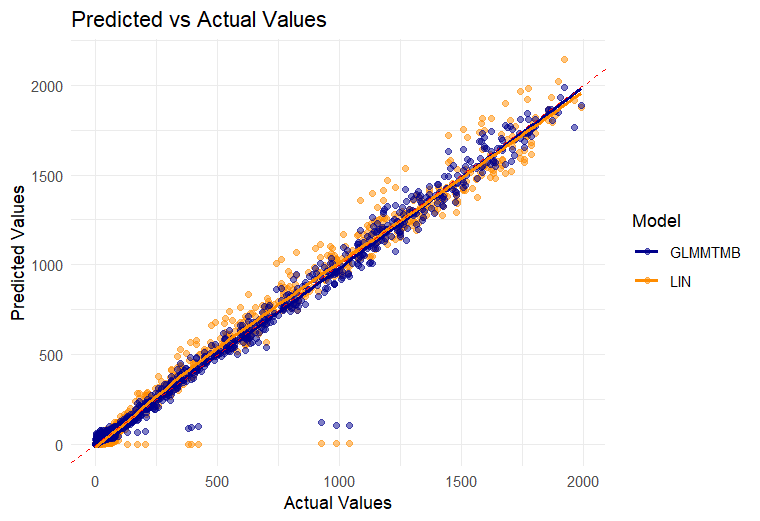
\includegraphics[width=0.8\textwidth]{visuals/mortalityData/mortpredvactLIN.png}
\caption*{Loess-smoothed plot comparing predicted versus actual values.}
\label{fig:hist_pred_errors}

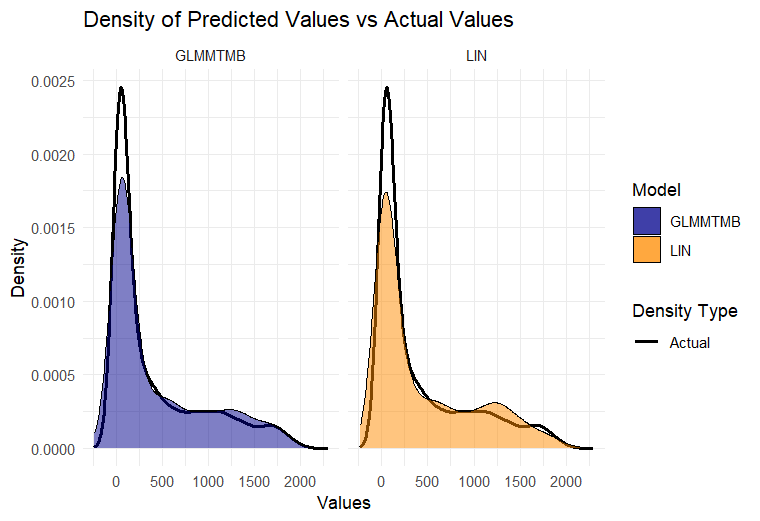
\includegraphics[width=0.8\textwidth]{visuals/mortalityData/mortdenspredvactLIN.png}
\caption*{Predicted vs Actual Densities.}
\label{fig:predicted_vs_actual_densities}

\caption{Performance on Test Data for Death Count - Linear vs Splines}
\label{fig:test_data_performance_4}
\end{figure}

From the comparison with and without spline components we see that the accuracy increases, with the RMSE being lower for the blue \texttt{glmmTMB}-model. From the plots we see that there is a wider spread from the actual values with the linear model, predicting higher values continuously with the actual value increases. Considering this we will move on with comparing the model with spline components in a \texttt{gamm4}-model.




\begin{table}[H]
\centering
\caption{Model Evaluation Results}
\label{table:model_evaluationmort}
\begin{tabular}{lcc}
\hline
\textbf{Model} & \textbf{Cross Validation RMSE} & \textbf{Test Data RMSE} \\
\hline
gamm4 &  90.70  & 92.38 \\
glmmTMB & 58.62 & 60.30 \\
\hline
\end{tabular}
\end{table}

\begin{figure}[H]
\centering

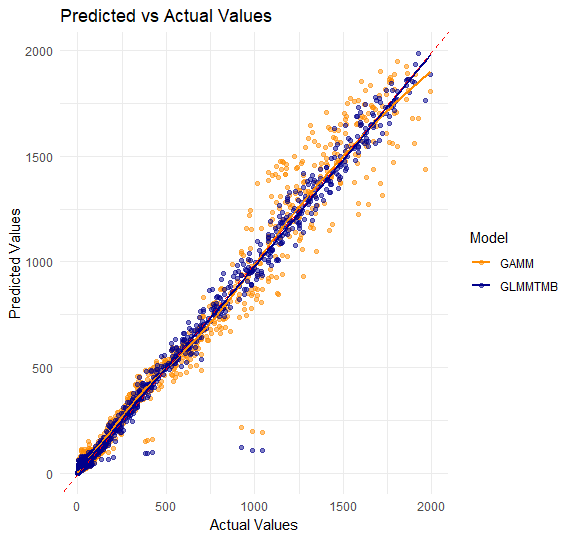
\includegraphics[width=0.7\textwidth]{visuals/mortalityData/mortpredvact.png}
\caption*{Loess-smoothed plot comparing predicted versus actual values.}
\label{fig:hist_pred_errors}

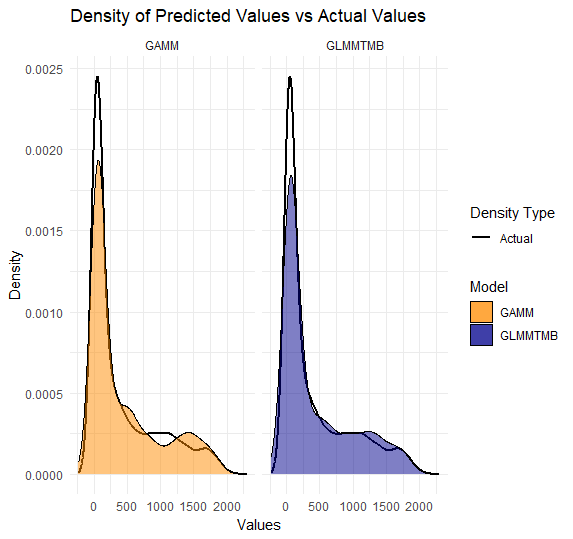
\includegraphics[width=0.7\textwidth]{visuals/mortalityData/mortdenspredvact.png}
\caption*{Predicted vs Actual Densities.}
\label{fig:predicted_vs_actual_densities}

\caption{Performance on Test Data for Death Count}
\label{fig:test_data_performance_4}
\end{figure}

We see that from the inclusion of the dispersion parameter age our \texttt{glmmTMB}-model covers the larger values much better than our \texttt{gamm4}-model. We can also see that the \texttt{gamm4}-model covers the zero value slightly better, but as the rmse shows, the \texttt{glmmTMB}-model performs better overall.

Having the variable age as a dispersion parameter is the advantage that makes \texttt{glmmTMB} the better model in this instance. The nbinom2 family in \texttt{glmmTMB} will automatically find the dispersion parameter while the negbin family needs manually input which is also a feature that makes \texttt{glmmTMB} the more user friendly model.


\subsection{Death Rates}\label{sec:analysis:death_rate}

The death rates described in the data set are the death count divided by the amount of people observed exposed and at risk. For modeling of this percentage we thought it would be a good pre-processing measure to include only the data where the rate is in the finite interval between zero and one. This would reduce the data set by about 2,5 percent to 5725 observations, and we could now use the beta distribution often used for percentages. One of the downsides of this though might be the use of the death count as a zero-inflation parameter. As we do not use the death counts as a parameter we will include it as a random effect after grouping the counts to different levels in a new variable.

\subsubsection{Model Selection}
We are using this example to show the flexibility of family distributions in \texttt{glmmTMB} compared to a \texttt{gamm4}-model. Where as \texttt{glmmTMB} have implemented the beta distribution as a family, our best shot at making a model in \texttt{gamm4} would be to use a logit-transformation to be able to model with a gaussian distribution. We of course later back-transform the prediction so it is comparable with our other model. We tried various dispersion parameters that made for a good AIC, but the rmse did not show a good performance. Using age as a dispersion parameter caused convergence issues for this response variable, but even though using a scaled age-variable helped, it did not prove to become a better model.
\newline
Instead we made our own variable for the level of deaths that we could use as a random effect. Dividing the counts into 5 levels made for a slightly better model looking at the performance measures. Since we could not compare the models as usual we compared to a normal \textbf{gamm}-model at first, which was identical to our \texttt{glmmTMB}-model before we added random effects.



\begin{lstlisting}[language=R][language=R]
gamm4(q_male_logit~ s(Age€ + s(Year€,
                   random=~(1|death_count_group€,
                   family=gaussian(€,
                   data = swedish_mortality1€ 


glmmTMB(q_male ~ s(Year€ + s(Age€
               + (1|death_count_group€,
                 family=beta_family(link = "logit"€, 
                 data = swedish_mortality1€
\end{lstlisting}

\subsubsection{Results}

\begin{table}[H]
\centering
\caption{Model Evaluation Results}
\label{table:model_evaluationmort}
\begin{tabular}{lcc}
\hline
\textbf{Model} & \textbf{Cross Validation RMSE} & \textbf{Test Data RMSE} \\
\hline
gamm4 & 0.0619  & 0.0668 \\
glmmTMB & 0.0365 & 0.0417 \\
\hline
\end{tabular}
\end{table}

\begin{figure}[H]
\centering

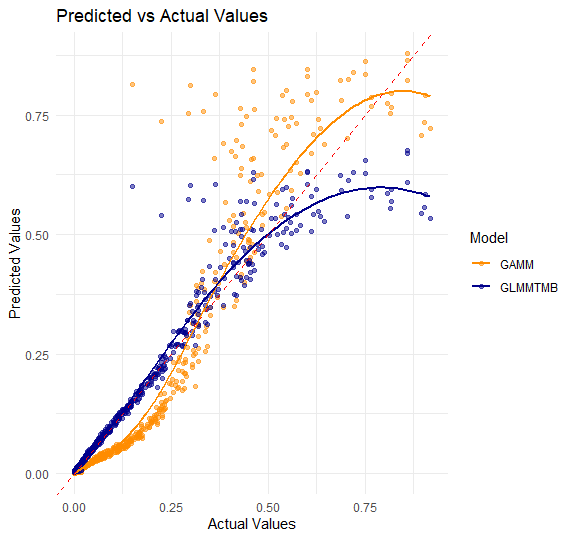
\includegraphics[width=0.7\textwidth]{visuals/mortalityData/predvactRATE.png}
\caption*{Loess-smoothed plot comparing predicted versus actual values.}
\label{fig:hist_pred_errors}

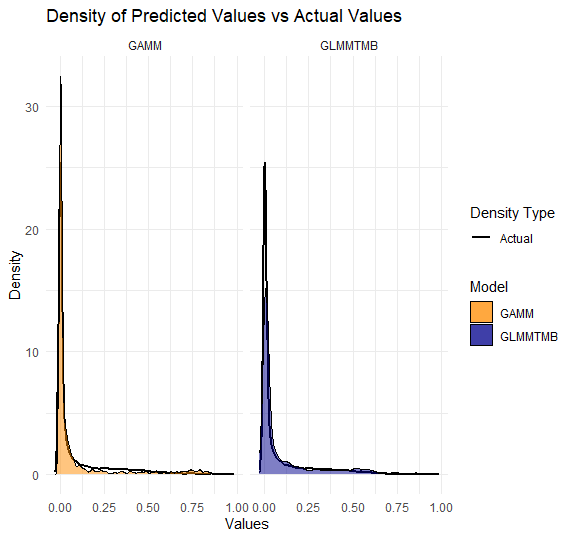
\includegraphics[width=0.7\textwidth]{visuals/mortalityData/denspredvactRATE.png}
\caption*{Predicted vs Actual Densities.}
\label{fig:predicted_vs_actual_densities}

\caption{Performance on Test Data for Death Rate}
\label{fig:test_data_performance_4}
\end{figure}

We can see that our back-transformed \texttt{gamm4}-model predicted heavily in the lower values and did not provide enough information at the tail of the density. Even though the \texttt{glmmTMB}-model did not cover all of the lower values, it had a lot better information of the tail of the distribution, as we can also tell from the rmse.


Our \texttt{glmmTMB}-model performs pretty good until the values of around 0.6. This could be explained by the small proportion of values we have between 0.5 and one. Unlike when modeling with death counts we did not have good enough variables to account for the extreme values. 
\newline
However, our main goal for predicting the death rate was including the beta distribution, as it is implemented in \texttt{glmmTMB} but not in \texttt{gamm4} and \texttt{gamm}. So, even though our results were better than using a back-transformed gaussian distribution, we would like to emphasize the flexibility \texttt{glmmTMB} gives us and its user-friendly setup not found in comparable packages.



\newpage

\section{Ridge Models in 
\texttt{glmmTMB}}\label{sec:ridge_models}

As we've come to learn, in \texttt{mgcv} and other frameworks whose smooth functionality relies on its machinery, the default approach is an Integrated Squared Second Derivative (ISSD) penalty, combined with Generalized Cross-Validation (GCV) for the selection of the smoothing parameter, and Maximum Likelihood Estimation (MLE) for model fitting. This combination, while standard, has shown a tendency to undersmooth (overfit) for complex models \citep{wood2017}. Although using REML for model fitting instead of MLE can greatly alleviate this problem, it brings additional computational burden and may still be insufficient for high-dimensional models with multiple smooth predictors where multicollinearity is also a potential consideration.
\newline

We propose that a Ridge approach could be used to robustly protect against undersmoothing a d collinearity  in these circumstances, due its effective global penalization directly on parameter coefficients. More specifically we hypothesise that a specific combination of smoother, regularization, smoothness selection and model fitting routine can provide a comparatively computationally efficient method for fitting well-regularized spline regression models in \texttt{glmmTMB}. This combination of steps is shortly summarized as:

\begin{enumerate}
    \item Construct a smooth object from cubic smoothing splines.
    \item Covert the smoother to a random effect representation.
    \item Specify the smooth object (basis function matrix \texttt{Xr}) as a fixed effect.
    \item Use GCV for smoothness ($\lambda$) selection.
    \item Fit the model using MLE.
\end{enumerate}

It's a primary goal in most modern analytic software to offer robust and flexible frameworks that don't require deep domain knowledge or technical modeling expertise from the user. Automatic regularization is a requirement for ease of use by reducing the need for intricate decisions based on domain understanding or the intricacies of the data. The current frameworks (which rely on \texttt{mgcv} machinery) have options and control over the regularization, but it's primarily rather advanced options related to the properties of the penalty matrix and structure of covariance matrices. Additionally, the actual regularization method is constrained to penalization of excess curvature (ISSD). Adding (implementing) an option for an automatic Ridge penalty will further increase the flexibility of the \texttt{glmmTMB} package. The Ridge approach can be a superior alternative for predictive analytics, like forecasting models, where the end goal is often about achieving the highest prediction accuracy possible with reasonably good computational efficiency, even if it means sacrificing some level of interpretability and local control. More user friendly options provide a better platform for non-expert users to effectively train and test a wider range of models, and thus an increased likelihood of obtaining a good model for the particular task at hand. 
\newline

\subsection{Regularization Effects}\label{sec:penunpencompare}

We've discussed much about regularization and penalties in complex models on the theoretical level in \ref{sec:smooth:penreg:penreg}. We should provide a simple example to demonstrate how penalization impacts accuracy and overfitting in spline regression models in practice. 

As we've mentioned in chapter 2, overfitting prevention is usually addressed through two primary approaches: \textbf{implicit regularization} and \textbf{explicit penalization}. The following table outlines the key characteristics of these approaches:

\begin{table}[H]
\centering
\begin{tabular}{|p{0.45\linewidth}|p{0.45\linewidth}|}
\hline
\textbf{Implicit/Local Control Regularization} & \textbf{Explicit Penalization} \\ \hline
\textbf{Variable selection:} A basic form of implicit regularization is choosing to only include the variables which explain the majority of the variance and contribute most to the models predictive power & \textbf{Penalization of Wigglyness/Curvature:} A penalty on the curvature (second derivative) of the spline, such as the Integrated Squared Second Derivative (ISSD), ensures a smoother curve by discouraging excessive bending. \\ \hline
\textbf{Number and location of Knots:} The number of knots directly affects the spline's flexibility. An appropriate number balances flexibility and overfitting. Strategic placement of knots in areas with more data variation can improve the model's fit without increasing its complexity unnecessarily.  & \textbf{Penalization of Coefficient Size (Ridge Penalty):} A quadratic penalty (like Ridge) on the spline coefficients prevents overfitting by constraining their magnitude, leading to a more robust model. \\ \hline
\textbf{Basis Functions:} An optimal choice of basis functions, like TPRS or cubic smoothing splines, (which have different degrees of inherit wigglyness / smoothness), can strike a balance between flexibility and smoothness. &  \textbf{Penalization of Variance (PCR):} Indirectly penalize variance (complexity) by focusing on the principal components that explain the most of the variance in the predictors. Often used for support vector machines (SVM) \\ \hline
\end{tabular}
\caption{Comparison of Implicit/Local Control Regularization and Explicit Penalization in Spline Regression}
\label{tab:regularization_penalization}
\end{table}

The combination of implicit/local control regularization and explicit penalization offers a compounded approach to model regularization. This dual strategy enhances the model's ability to balance complexity and overfitting. Implicit regularization, achieved through selecting knots and basis functions, establishes the foundational structure of the model, moderating its flexibility. Explicit penalization then complements this by targeting residual issues of excessive curvature or unduly large coefficients that may persist even after implicit regularization. By integrating these methods, we effectively compound their effects, ensuring a more nuanced control over the model. This synergy not only captures the data's underlying trends more accurately but also enhances the model's robustness and generalizability, particularly in complex statistical scenarios.

\subsection{Comparing Implicitly vs Explicitly Penalized Models}\label{sec:penunpencompare:compare}

Here we'll compare four different models all fitted on the same simulated data where the predictor is a linear function of the predictor plus a random noise term. We should expect the three models which initially have very much flexibility (thin plate splines with 50 degrees of freedom) to overfit the data severely if they are not subject to regularization. The model using cubic smoothing splines and only 5 degrees of freedom in the spline should inherently have much less flexibility, but may still overfit compared to a linear model.

\begin{lstlisting}[language=R]
tmb1 <- death ~ s(tmpd, k = 50€, data = train_data€
tmb2 <- death ~ homdiag(Xr_tmpd_tmb2|ID€, data = train_data€
tmb3 <- death ~ 1 + Xr_tmpd_tmb3, data = train_data€
tmb4 <- death ~ 1 + Xr_tmpd_tmb4, data = train_data€
\end{lstlisting}

\begin{itemize}
    \setlength{\itemsep}{1em} % Adjust the space between items
    \item \texttt{tmb1}: Standard implementation in glmmTMB. Rigorous implementation, which is equivalent to \texttt{gamm4}. Smoother and penalty matrix as in \texttt{mgcv::gamm}. Explicit ISSD penalty applied.
    \item \texttt{tmb2}: Manual method using the \texttt{s2rPred} function and a manually specified \texttt{homdiag} structure. The spline has \texttt{k = 50, bs="tp"}. This method also explicitly applies the ISSD penalty similarly to the example above. 
    \item \texttt{tmb3}: Simply fitting the random basis function matrix of the smooth term as a fixed effect (k = 50, bs = "tp"). No explicit or implicit regularization.
    \item \texttt{tmb4}: Similar to the above, but with more carefully chosen knot and basis function selection choices. The smooth has \texttt{k = 5, bs="cs"}. This smoother is implicitly regularized, with no explicit penalty applied. 
\end{itemize}

From figure \ref{fig:predicted_vs_actual_reglines_tmb1234} we can see  that clearly the unpenalized model, \texttt{tmb3}, is not performing well on the test data, showing clear overfitting. There are certainly some differences between the other models as well, which would be become more apparent on different data, however, here they all stay quite close to the true trend in the data, which is a straight line, which is the key takeaway from this example.


\begin{figure}[H]
    \centering
    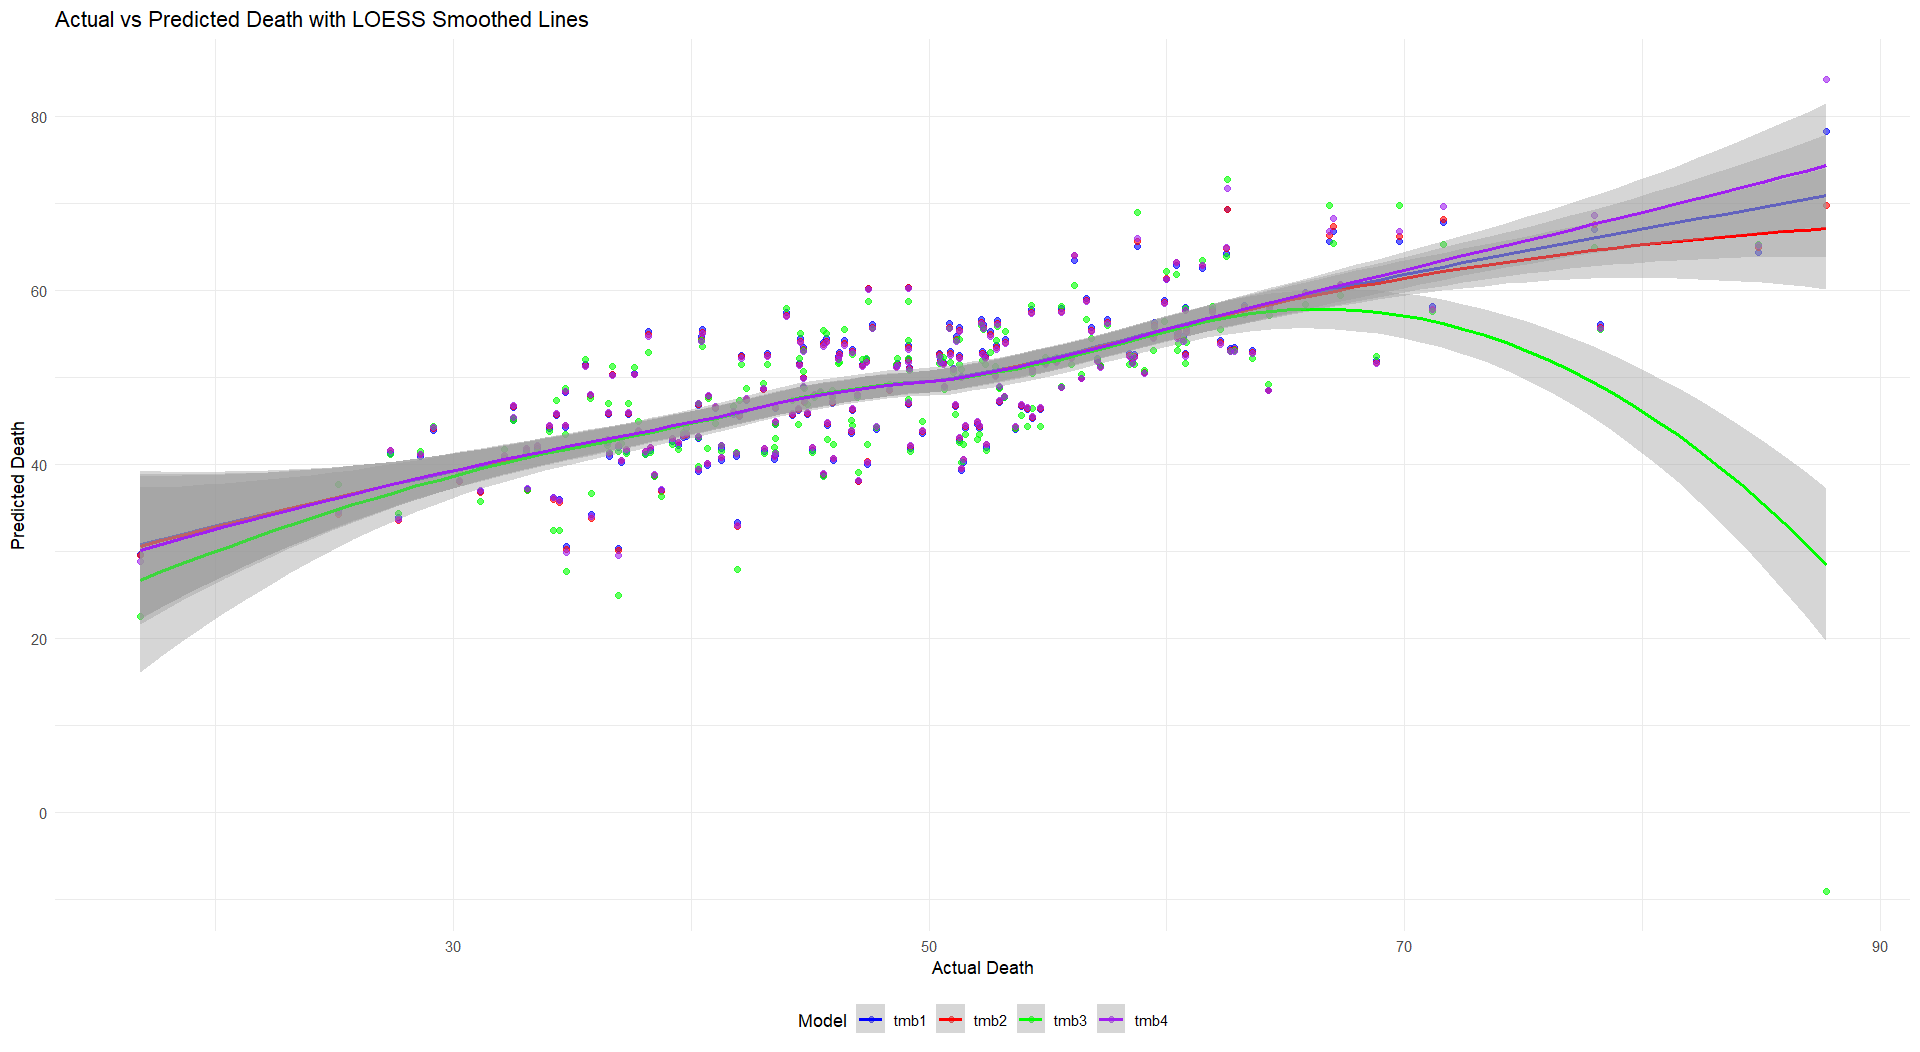
\includegraphics[width=0.9\textwidth]{visuals/Theory/overfit_tmb1234_pred_vs_act.png}
    \caption{Predicted vs actuals values on unseen test data of \texttt{tmb1, tmb2, tmb3 and tmb4}.}
    \label{fig:predicted_vs_actual_reglines_tmb1234}
\end{figure}

\subsection{Implementing Ridge Regularized GAMs}

\subsubsection{Smooths as Fixed Effects}\label{sec:ridge:smooth2random}

We've already at length analyzed and presented how smooths can be dual to random effects in \ref{sec:gaussian_random_quad_pen_smooth_equal} and later in \ref{sec:smooths:re:parametrization}. In the following models we will as mentioned in \ref{sec:ridge_models} estimate the smooths as fixed effects. The specific method is as follows: 

\begin{enumerate}
    \item Construct a smooth using cubic smoothing spline basis functions. \texttt{Xr} basis function matrix contains smooth entirely.
    \item We re-parameterize and define the smoother variable \texttt{Xr\_time} by extracting the random component, which in the case of the cubic smoothing spline, is the entire smooth object generated by \texttt{mgcv}. 
    \item We fit the model with the smooth estimated as a fixed effect. 
\end{enumerate}

Example code:

\begin{lstlisting}[language=R]
sm_time <- mgcv::smoothCon(s(time, bs="cs"€, 
absorb.cons = TRUE, data = fit_data€[[1]]
re_time <- mgcv::smooth2random(sm_time, "", type = 2€
pred_matrix_time <- s2rPred(sm_time, re_time, 
data = fit_data€
fit_data$Xr_time <- pred_matrix_time$rand[[1]]
gam <- glmmTMB(log_ret ~ Xr_time, data = fit_data€
\end{lstlisting}

The idea here is that for smooths constructed from a cubic smoothing spline, has no null space, and hence "random" part, the \texttt{Xr} basis function matrix contains the entire smooth. Estimating the smooth as a fixed effect greatly enhances the efficiency and still captures the information from the smooth object, which can flexibly adapt to non-linearity in the data. However, recalling from the example in \ref{sec:penunpencompare}, this smooth is now not subjected to any explicit penalty, and is highly likely to overfit. This is why we will impose a Ridge penalty on the model globally, which is the next step.

\subsubsection{Implementing a Ridge Penalty}

We will implement a Ridge penalty for (all) the smoother(s) to make sure our model becomes smooth and robust to overfitting. This is done through a series of steps:

\begin{enumerate}
    \item Implement a function \texttt{calculate\_n\_knots} to calculate the number of knots for smooth terms based on their rank or dimensionality.
    \item Define \texttt{augment\_design\_matrix} and \texttt{augment\_response} functions to augment the design matrix and response vector, respectively, incorporating the Ridge penalty via an augmented matrix construction.
    \item Implement \texttt{augment\_data} to augment data with penalized smooth terms, preparing it for model fitting with \texttt{glmmTMB}.
\end{enumerate}

The essential operation of the Ridge penalty is done in the augmentation functions, which in simple terms append rows at the bottom of the model matrices. The rows are constructed by taking the square root of the smoothing parameter $\lambda$ and multiplying it by the identity matrix of equal rank. For a design matrix this corresponds to 
\begin{equation}
\text{Augmented}\; X_r = \left[\begin{array}{cc}
     Xr \\
     \sqrt{\lambda} \cdot \mathbf{I} 
\end{array}\right]    
\end{equation}

Example code for a slightly more involved implementation with parallelization and multiple covariates: 

\begin{lstlisting}[language=R]

    
covariates <- c("time", "volume", "seasonal", "trend"€

calculate_n_knots <- function(smooth_term€ {
  if (!is.null(smooth_term[["rank"]]€€ {
    # For tensor product smooths, use the first element of 'rank'
    return(smooth_term[["rank"]][1]€
  } else {
    return(smooth_term[["bs.dim"]] - smooth_term[["null.space.dim"]]€
  }
}

generate_smooth_terms <- function(covariate, data, bs = "tp", k) {
  # Ensure that k is provided
  if (is.null(k€€ stop("The 'k' argument 'number of knots' must be provided."€
  formula_str <- paste0("s(", covariate, ", bs='", bs, "', k=", k, "€"€
  sm_formula <- eval(parse(text = formula_str€€
  sm <- mgcv::smoothCon(sm_formula, data = data, absorb.cons=TRUE€[[1]]
  re <- mgcv::smooth2random(sm, "", type = 2€
  pred_matrix <- s2rPred(sm, re, data = data€
  
  # Return the necessary components
  list(Xf = pred_matrix$Xf, Xr = pred_matrix$rand[[1]], n_knots = calculate_n_knots(sm€€
}
results <- future_map(covariates, ~generate_smooth_terms(.x, data = fit_data, bs = "cs", k = 5€€

for (i in seq_along(covariates€€ {
  covariate <- covariates[i]
  fit_data[[paste0("Xf_", covariate€]] <- results[[i]]$Xf
  fit_data[[paste0("Xr_", covariate€]] <- results[[i]]$Xr
  fit_data[[paste0("n_knots_", covariate€]] <- results[[i]]$n_knots
}
n_knots_list <- setNames(lapply(results, `[[`, "n_knots"€, covariates€

augment_design_matrix <- function(Xr, lambda€ {
  if (is.null(Xr€ || nrow(Xr€ == 0 || ncol(Xr€ == 0) {
    stop("Input matrix Xr is NULL or empty"€
  }
  tryCatch({
    augmented_matrix <- rbind(Xr, sqrt(lambda€ * diag(ncol(Xr€€€
    if (is.null(augmented_matrix€ || nrow(augmented_matrix€ == 0€ {
      stop("Augmented matrix is NULL or empty after applying ridge penalty"€
    }
  }, error = function(e€ {
    stop(paste("Error in augment_design_matrix: ", e$message€€
  }€
  
  return(augmented_matrix€
}

augment_response <- function(y, augmented_length) {
  c(y, rep(0, augmented_length - length(y€€€
}

augment_data <- function(data, lambda, n_knots_list) {
  augmented_matrices <- list(€
  
  for (name in names(n_knots_list€€ {
    xr_var <- data[[paste0("Xr_", name€]]
    if (is.null(xr_var€€ {
      stop(paste0("Variable ", paste0("Xr_", name€, 
      " is NULL"€€
      }
    augmented_matrix <- augment_design_matrix(xr_var,
    lambda€
    augmented_matrices[[name]] <- augmented_matrix
  }
  
  y_augmented <- augment_response(data$log_ret, 
  max(sapply(augmented_matrices, nrow€€€
  
  augmented_data <- data.frame(log_ret = y_augmented€
  # Ensure correct response variable name
  for (name in names(n_knots_list€€ {
    augmented_matrix <- augmented_matrices[[name]]
    augmented_data[[paste0("Xr_", name€]] <- I(augmented_matrix€
  }
  return(augmented_data€
}
\end{lstlisting}\label{rcode:ridge_penalty}

\subsubsection{Smoothness Selection}

The next step is to find the appropriate strength for the Ridge penalty, that smooths the model sufficiently that the model doesn't overfit the data, but also doesn't oversmooth the model such that it is unable to capture non-linear patterns when present. 
\newline

Our method for doing this is by generalized cross validation (GCV). Recall from \ref{sec:smooth:lambda:gcv} that GCV is an efficient method for this purpose. We implement GCV by the following steps: 

\begin{enumerate}
    \item Define the function \texttt{gcv\_lambda} to compute a Generalized Cross-Validation score for a given lambda, using a \texttt{glmmTMB} model fit on the augmented data.
    \item The function \texttt{cross\_validate\_lambda\_with\_early\_stopping} performs cross-validation over a range of lambda values to find the optimal lambda, using early stopping to prevent overfitting and decrease time usage.
    \item Augment the data (to be used for the model fitting) using the optimal lambda identified through cross-validation, applying Ridge penalization to the smooth terms.
\end{enumerate}

Example code (continuation of the code in \ref{rcode:ridge_penalty})

\begin{lstlisting}[language=R]
    
gcv_lambda <- function(lambda, n_knots_list, data€ {
  augmented_data <- augment_data(data, lambda, n_knots_list€
  
  gcv_model <- glmmTMB(log_ret ~ 1 + Xr_time + Xr_volume + Xr_trend + Xr_seasonal, 
  data = augmented_data, family = gaussian(link="identity"€€
  
  log_likelihood <- logLik(gcv_model€
  edf <- attr(log_likelihood, "df"€
  deviance_val <- deviance(gcv_model€
  N <- nrow(augmented_data€
  gcv_score <- deviance_val / ((1 - edf/N)^2€
  return(gcv_score€
}

cross_validate_lambda_with_early_stopping <- function(data, lambda_values, n_knots_list, early_stopping_rounds = 5€ {
  require(future.apply€
  plan(multisession, workers = 5€
  best_score <- Inf
  scores <- numeric(length(lambda_values€€
  no_improvement_count <- 0
  
  for (i in seq_along(lambda_values€€ {
    lambda <- lambda_values[i]
    score <- gcv_lambda(lambda, n_knots_list, data€
    scores[i] <- score
    
    if (score < best_score€ {
      best_score <- score
      no_improvement_count <- 0
    } else {
      no_improvement_count <- no_improvement_count + 1
      if (no_improvement_count >= early_stopping_rounds€ {
        message(sprintf("Early stopping after %d iterations", i€€
        break
      }
    }
  }
  
  scores <- scores[1:i]  # Truncate the scores vector to actual number of iterations
  lambda_values_truncated <- lambda_values[1:i]  # Truncate lambda values to match the scores length
  
  list(optimal_lambda = lambda_values[which.min(scores€], gcv_scores = scores, lambda_values = lambda_values_truncated€
}

plan(sequential€
gc(€
options(future.seed = TRUE, future.rng.onMisuse="ignore"€

lambda_values <- seq(0.00001, 1, by = 0.05€
cv_results <- cross_validate_lambda_with_early_stopping(fit_data, lambda_values, n_knots_list, early_stopping_rounds = 5€
optimal_lambda <- cv_results$optimal_lambda
gcv_values <- cv_results$gcv_scores
lambda_values_used <- cv_results$lambda_values

fit_data_augmented <- augment_data(fit_data, optimal_lambda, n_knots_list)
\end{lstlisting}

\subsubsection{Training and Validating Models}

From this point training, validating and testing the models are done similarly to the standard models. We split the data and define a few functions to facilitate model specifications, cross validation and extracting results. We use parallelization for most of the heavy computations for performance, so we have to be careful to restart the backend and free up memory after each major parallelized task. For large models, the memory requirement can escalate quickly with parallelized processes, so adjust the number of cores to be used accordingly. Full R program files for each model is available at \href{https://github.com/AllInCade/MasterProjecthttps://github.com/AllInCade/MasterProject}{GitHub}.
\newline

\textbf{Note:} Our R code to perform these steps and fit the Ridge models are just working examples intended for a proof of concept. Efficient and stable implementation into the source code of \texttt{glmmTMB} is beyond our abilities, and the scope of the thesis. 

\subsection{Data Analysis}

Revisiting a few of the datasets and models from chapter 8, we will now compare Ridge regularized models vs the standard method. We'll measure the RMSE and the time usage for each of the models and compare. 

\subsubsection{Bank Failure Estimated Loss}\label{sec:ridge:bank_model_ridge}

Recall the analysis in \ref{sec:analysis:bank_fail_cost} where we analyzed the estimated loss associated with bank failures. Here we analyze the data set again on the log transformed cost variable. 

We deploy the ridge regularization as described in earlier in the chapter, and formulate the following models.
\textbf{Note:}The generalized cross validation process for selecting the smoothing parameter took 5 seconds. However, it's only performed once, and can be optimized far more than it currently is, by using only a subset of the data.

\begin{lstlisting}
manual_formula <- formula(log_COST ~ 1 + Xr_TIME + 
                Xr_log_ASSET + Xr_DEP_ASS_RATIO +
                Xr_CERT + Xr_FIN + Xr_log_DEPOSIT€
manual_family <- gaussian(link = "identity"€

auto_model <- formula(log_COST ~ s(TIME€ + 
           s(log_ASSET€ + s(log_DEPOSIT€ +
           s(DEP_ASS_RATIO€ + s(CERT) + s(FIN€€
auto_family <- gaussian(link = "identity"€
\end{lstlisting}

The results are quite favorable for the ridge models, as seen in the table and plot below. 
 
\begin{table}[H]
\centering
\begin{tabular}{lccc}
\toprule
\textbf{Model} & \textbf{RMSE} & \textbf{Training Time (s)} & \textbf{Prediction Time (s)} \\
\midrule
ManualModel & 1.559 & 0.85 & 0.27 \\
AutoModel   & 4.996 & 23.90 & 2.17 \\
\bottomrule
\end{tabular}
\caption{Bank Failure: Comparison of RMSE, Training Time, and Prediction Time for ManualModel and AutoModel}
\label{tab:model_comparison}
\end{table}

\begin{figure}[H]
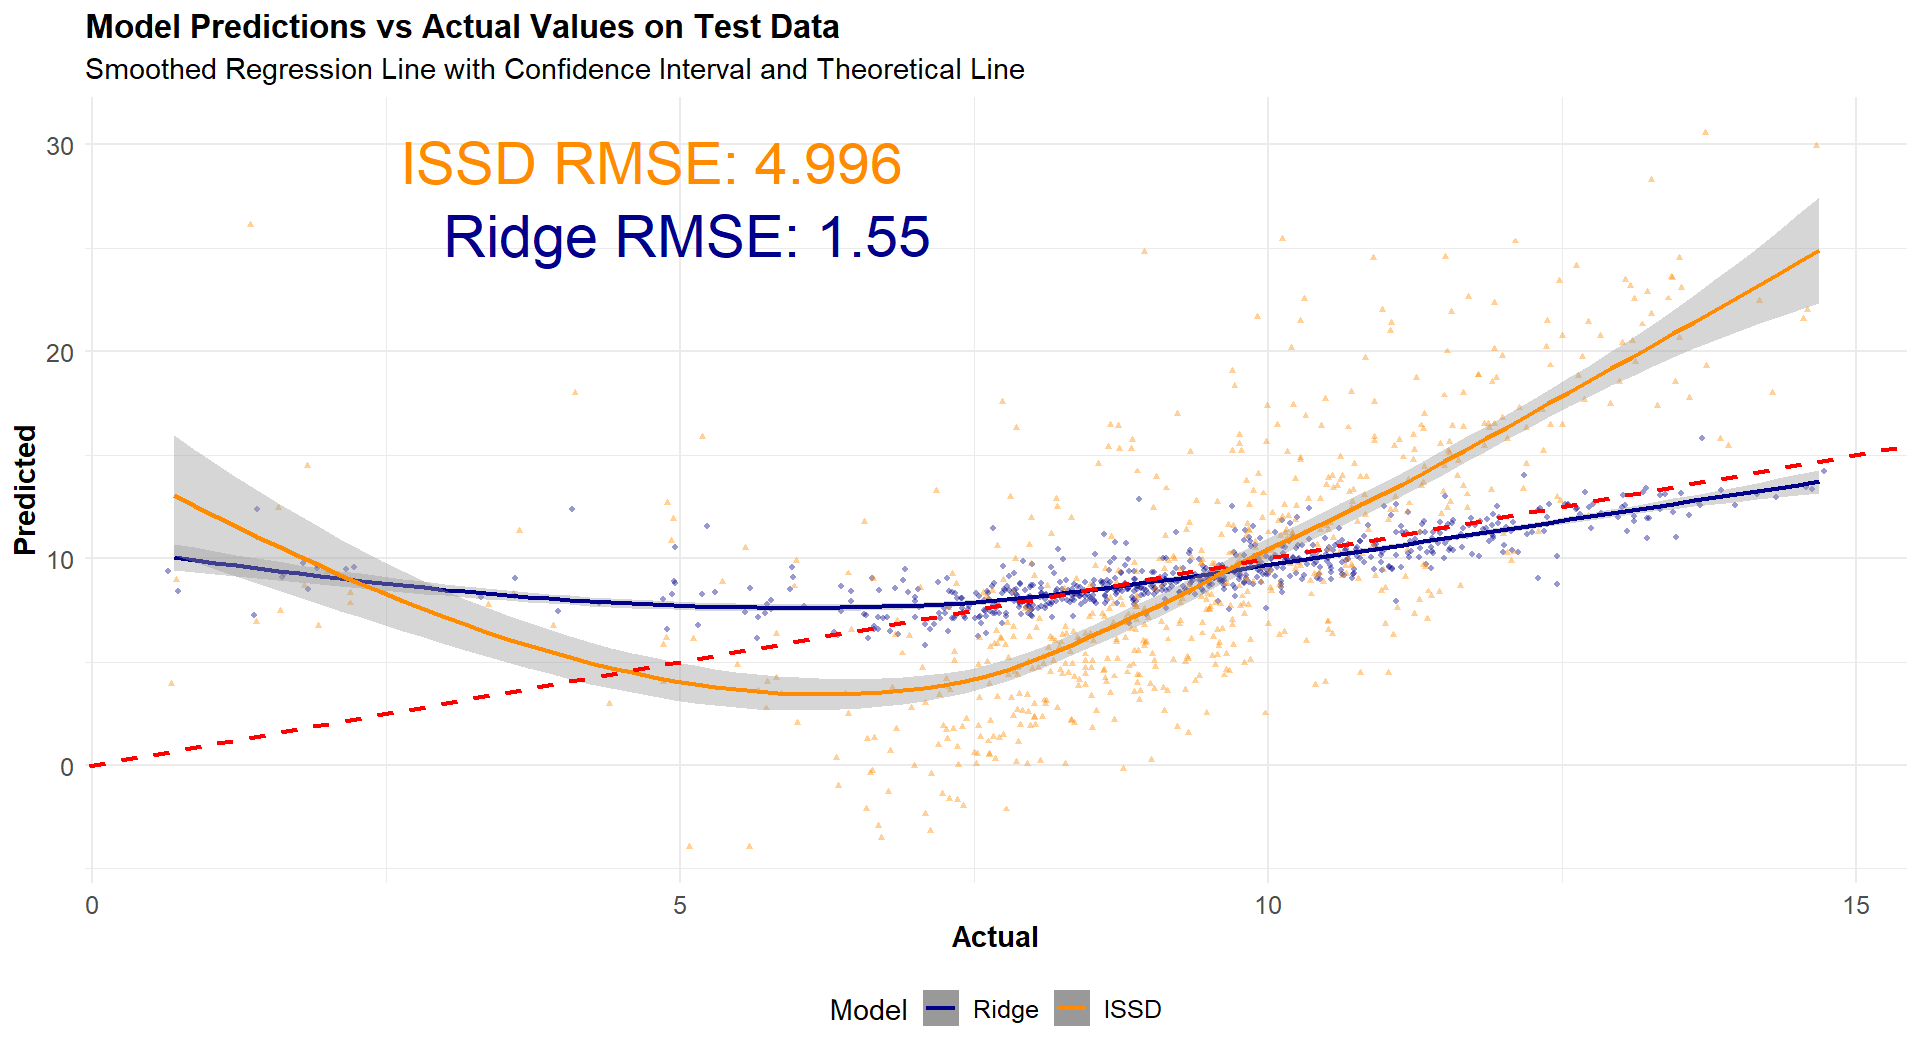
\includegraphics[width=\textwidth]{visuals/ridge/loess_ridge_issd_new.png}
\caption{Test Data Predictions vs Actuals with loess smoothing for Bank Failures}
\label{loess_bank_ridge}
\end{figure}

Explaining the differences in performance is easy with respect to the time usage, but more subtle and difficult to diagnose when it comes to the accuracy aspect. It's worth mentioning that the GCV chose a large $\lambda$ value for this data, so that the ISSD regularized (auto) model is undersmoothed is likely the cause. We also observe that there is collinearity between the ASSET and DEPOSIT variables, which is likely handled better by the ridge penalty. 

\subsubsection{Log Return III}\label{sec:ridge:wind_model_ridge}

Now we re-visit the data from \ref{sec:analysis:timeseries} and a slightly simpler version of the models from \ref{sec:analysis:alt_mod}. We'll fit the model using smoothers for all the predictors we include. We we perform some analysis using a random forest and \texttt{glmnet} lasso regression to identify the best predictors. We arrive at these models: 

\begin{lstlisting}
manual_model <- formula(N100_log_return ~ 1 + 
            Xr_time + Xr_N100_RSI_lag + 
            Xr_N225_log_return€
manual_family <- gaussian(link = "identity"€

auto_model <- formula(N100_log_return ~ s(time€ + 
           s(N100_RSI_lag€ + s(N225_log_return€€
auto_family <- gaussian(link = "identity"€
\end{lstlisting}

By the results we see that both models struggle to fit very accurately, but as we noted previously, predicting this type of data is inherently difficult and requires a lot of data and sophistication. That being said, the ridge model once again outperforms the default model. 

\newpage

\begin{table}[H]
\centering
\begin{tabular}{lccc}
\toprule
\textbf{Model} & \textbf{RMSE} & \textbf{Training Time (s)} & \textbf{Prediction Time (s)} \\
\midrule
ManualModel & 0.012 & 0.36 & 0.05 \\
AutoModel   & 0.030 & 3.16 & 0.25 \\
\bottomrule
\end{tabular}
\caption{Log Return: Comparison of RMSE, Training Time, and Prediction Time for ManualModel and AutoModel}
\label{tab:model_comparison}
\end{table}

\begin{figure}[H]
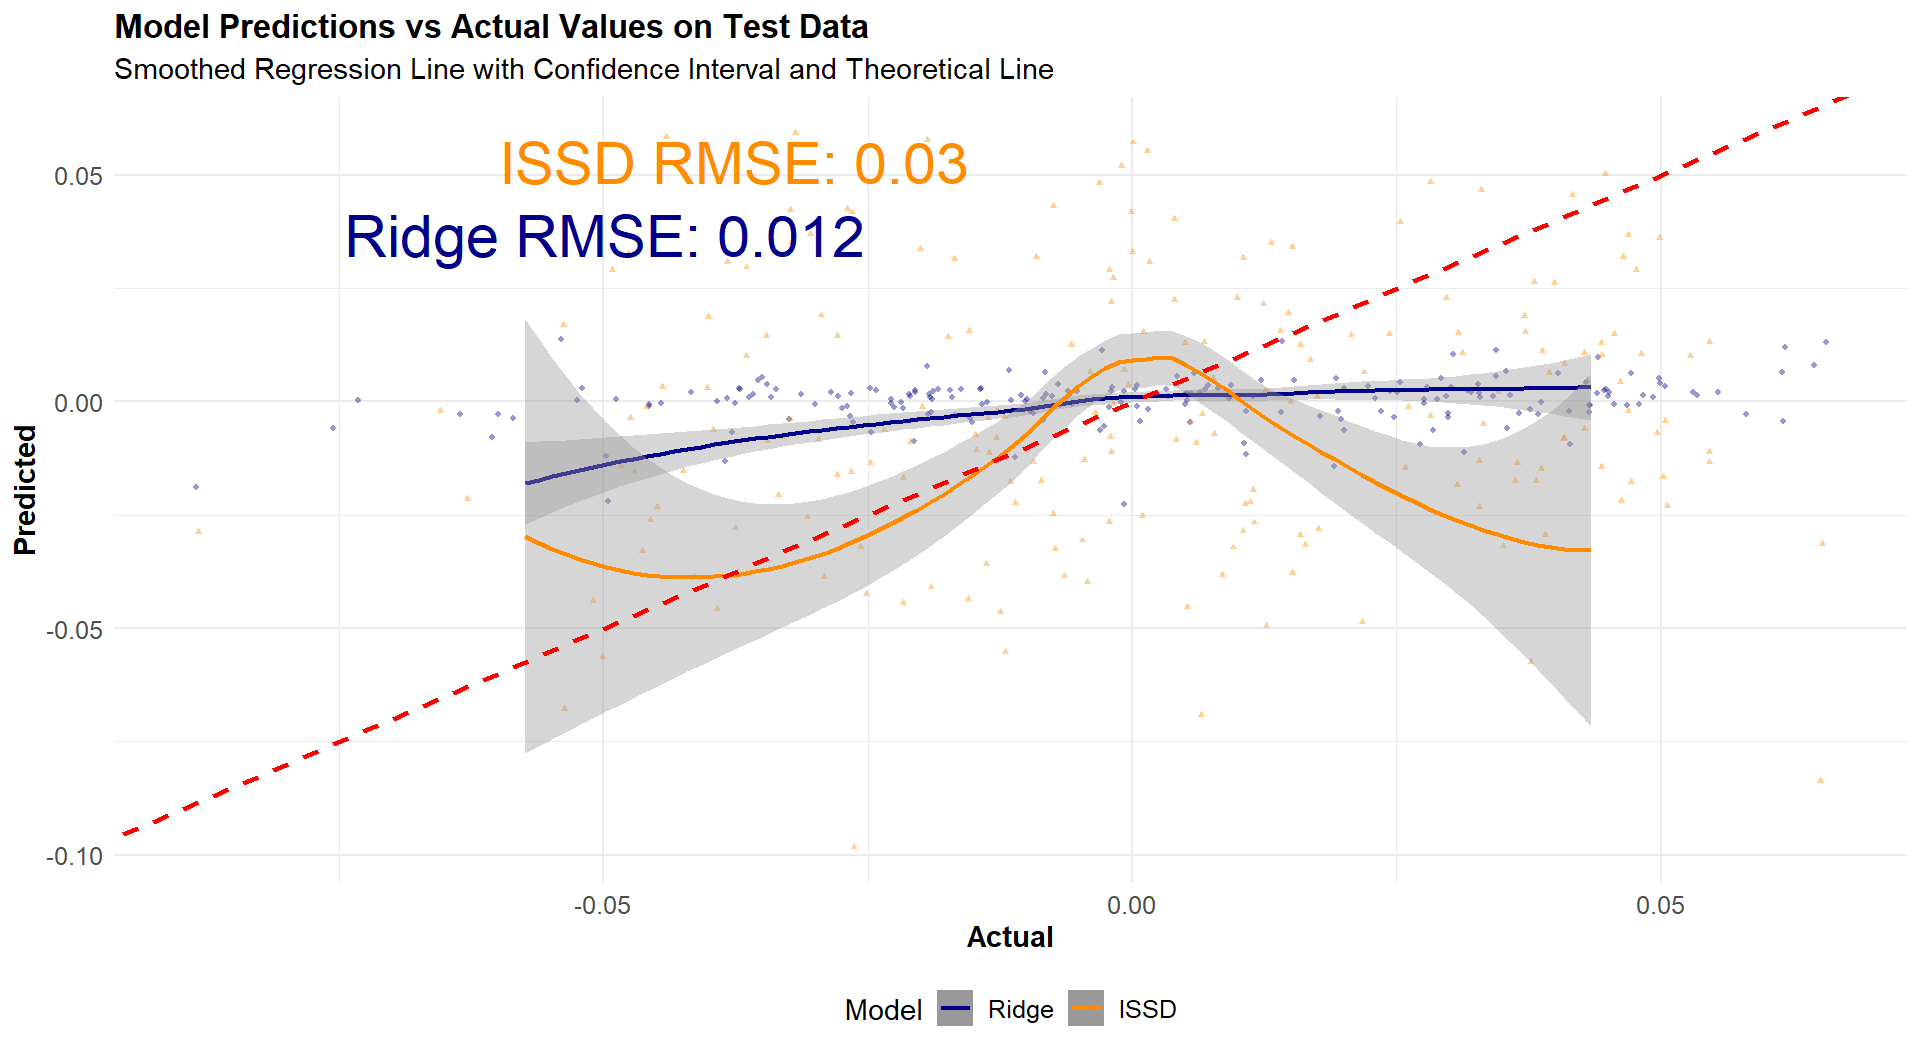
\includegraphics[width=\textwidth]{visuals/ridge/loess_issd_ridge_new.png}
\caption{Test Data Predictions vs Actuals With Loess Smoothing for Log Returns}
\label{loess_logreturn_ridge}
\end{figure}

We see a clear tendency that the ridge penalty constrains the parameter coefficient magnitudes to smooth the model more strongly than the curvature penalty from the default model does, which here results in better predictions. 

\subsubsection{Face Value}

In section \ref{sec:analysis:face_value} we encountered a data set with many extreme-valued variables. Using Face Value as a response variable seemed to be a problem for our modeling, with some zero values and a wide spread of positive values. We tried using the Tweedie distribution to account for these attributes with no luck, so we will now use gaussian to model as well to account for convergence issues. We will therefore try to use the Ridge penalty in search of a better model. The two explanatory variables were seemingly collinear, a problem the Ridge penalty should be better at handling, so we have the following models;


\begin{lstlisting}
manual_model_formula <- formula(Face ~ 1 +
                Xr_Income_log+Xr_TotIncome_log,
                data = augmented_data€
manual_model_family <- gaussian(link="identity"€

auto_model_formula <- formula(Face ~ s(Income_log€+
                    s(TotIncome_log€, 
                    data = augmented_data€
auto_model_family <- gaussian(link="identity"€

\end{lstlisting}

We can see by the results below that the models still seem to fit quite badly to the Face value, but looking at the performance metric there is a slight advantage for the Ridge penalty, possibly indicating that it handles the collinearity between the two explanatory variables better. The fact that the models largely fail to capture and predict the response is probably due to the data set not being good enough, i.e there just isn't enough good information to discern a strong and consistent pattern. 

\newpage



\begin{table}[H]
\centering
\begin{tabular}{lccc}
\toprule
\textbf{Model} & \textbf{RMSE} & \textbf{Training Time (s)} & \textbf{Prediction Time (s)} \\
\midrule
ManualModel & 81296.8 & 0.430 & 0.04 \\
AutoModel   & 81795.3 & 1.08 & 0.08 \\
\bottomrule
\end{tabular}
\caption{Face Value: Comparison of RMSE, Training Time, and Prediction Time for ManualModel and AutoModel}
\label{tab:Facemodel_comparison}
\end{table}

\begin{figure}[H]
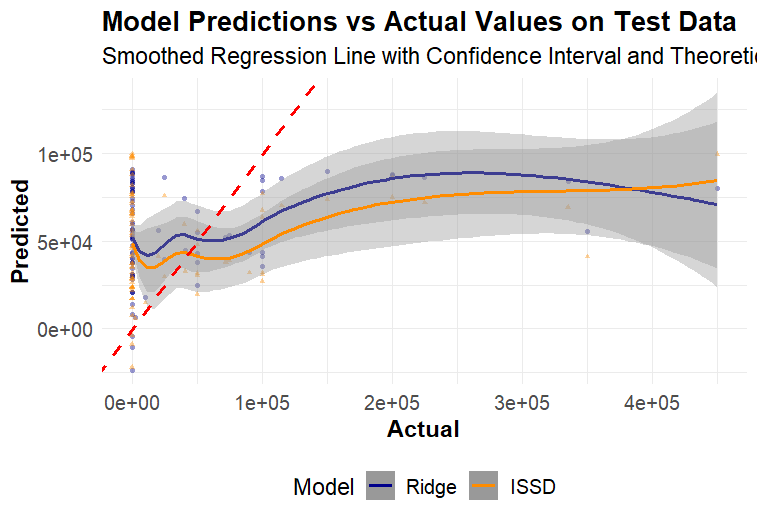
\includegraphics[width=\textwidth]{visuals/ridge/FaceValueRidgeplot.png}
\caption{Test Data Predictions vs Actuals With Loess Smoothing For Face Value.}
\label{loess_Face_ridge}
\end{figure}

We can see by the time that Ridge has an advantage also for smaller but extreme-valued data sets, while giving approximately the same results. In this case we can probably conclude with the problem being the data set, as we do not have enough information in our explanatory variables to predict the response. The two variables were the most important features when conducting a random forest and still did not perform good. In conclusion, this is clearly not the best example for the utilization of the penalty, but by the "No Free Lunch theorem" we also wanted to include an example showing that there is not always a best model.

\subsection{Time Complexity Analysis}

It's useful to get an estimate for how large the difference in performance (with respect to time usage) is between the models, and how they scale with data set size. Below is an analysis performed on the 'log return III' model using the same data, but filtered on import by the \texttt{from= "yyyy-mm-dd"} to regulate the size of the data set. We've used data up to 2024-01-01, and from 01-01 for 2002, 2006, 2010, 2014, 2018, 2020, and 2022. There are on average 252 trading days per year, so the number of observations are given somewhat approximately (less than 1\% off for all data sets). The training and prediction sets are split 80:20 respectively. 
\textbf{Note:} The time for initial GCV process is \textit{not} included in this data, which obviously skews the results. However, the GCV process is only performed once for a given model, doesn't take much time, and can be optimized much further.

\subsubsection*{Data}
\begin{table}[h!]
\centering
\begin{tabular}{|c|c|c|c|}
\hline
Model & $n$ & Training Time (s) & Prediction Time (s) \\
\hline
Ridge & 1000 & 0.36 & 0.05 \\
Auto & 1000 & 3.16 & 0.25 \\
Ridge & 1500 & 0.44 & 0.08 \\
Auto & 1500 & 4.6 & 0.41 \\
Ridge & 2500 & 0.55 & 0.13 \\
Auto & 2500 & 9.5 & 0.9 \\
Ridge & 3500 & 0.65 & 0.16 \\
Auto & 3500 & 11.7 & 1.21 \\
Ridge & 4500 & 0.8 & 0.19 \\
Auto & 4500 & 14.5 & 1.52 \\
Ridge & 5500 & 0.87 & 0.23 \\
Auto & 5500 & 19.6 & 1.9 \\
\hline
\end{tabular}
\caption{Training and Prediction Times for Ridge and Auto models}
\end{table}

\subsubsection*{Analysis}
Assuming a power law relationship, we have

\[
T_{\text{train}}(n) = k_{\text{train}} \cdot n^{a}
\]
\[
T_{\text{predict}}(n) = k_{\text{predict}} \cdot n^{b}.
\]

\subsubsection{Results} 

Computing the parameters using the \texttt{minpack.lm} package in R gives the following:
\newline

Training 
\[
T_{\text{train, Ridge}}(n) \approx 0.045 \cdot n^{0.43} = O(n^{0.43})
\]

\[
T_{\text{train, Auto}}(n) \approx 0.0037 \cdot n^{1.64} = O(n^{1.64})
\]

Prediction 
\newline
\[
T_{\text{predict, Ridge}}(n) \approx 0.005 \cdot n^{0.68} = O(n^{0.68})
\]

\[
T_{\text{predict, Auto}}(n) \approx 0.0005 \cdot n^{1.33} = O(n^{1.33})
\]
\newline

The scaling $S$ for each model is
\newline
\[
S_{\text{train}}(n) = \frac{T_{\text{train, Auto}}(n)}{T_{\text{train, Ridge}}(n)} = \frac{0.0037 \cdot n^{1.64}}{0.045 \cdot n^{0.43}} = 0.0822 \cdot n^{1.21} = O(n^{1.21})
\]

For prediction:
\[
S_{\text{predict}}(n) = \frac{T_{\text{predict, Auto}}(n)}{T_{\text{predict, Ridge}}(n)} = \frac{0.0005 \cdot n^{1.33}}{0.005 \cdot n^{0.68}} = 0.1 \cdot n^{0.65} = O(n^{0.65})
\]

It's clear by these results that the Ridge method, for this model, on this data, is vastly more efficient both in training and prediction. The difference is greatest for training, but is also highly significant for prediction. The scaling, or speedup factors, $1.21$ for training and $0.65$ for prediction, indicate clearly that for larger data sets, the relative difference in time consumption could be enormous. However, we should be careful with extrapolating power laws arbitrarily. 


\section{Discussion}\label{sec:discussion}

\subsection{Results of Interest}\label{sec:Results}

Our work on this project has been very valuable and instructive, to ourselves in particular, but we have also obtained some interesting results, which we will present and discuss below.

\paragraph{Cubic Smoothing Spline Basis Functions}

Cubic smoothing splines don't work in the current (1.1.9) \texttt{glmmTMB}-package. Section \ref{sec:makingsmooth:bs:prop} contains a proposition for an implementation method. Extending the spline options in \texttt{glmmTMB} to include cubic smoothing splines brings it more in line with other packages which rely on the same \texttt{mgcv} utilities. Implementing the changes to fix this big is fairly trivial, and there is no reason not to do it. More spline types to choose from provides more flexibility which is a general benefit. An implementation of our method as an option in the package would make the basis functions \texttt{"cs"} and \texttt{"cc"} work in \texttt{glmmTMB}, evidently making the package more "easy-to-use".

\paragraph{Smoother Parameterization}

The \texttt{mgcv::gam} function uses the "natural" parameterization for smooths, and all mixed model framework discussed in this paper \texttt{(glmmTMB, gamm4, gamm etc.)} use \texttt{mgcv::smooth2random} to re-parameterize the smooth object (\ref{sec:makingsmooth:smooth2random}). This re-formulation an re-structuring of the smooth results in a (slightly) different optimization problem (fitting the model in simple terms) which in turn yield different solutions, ultimately producing slightly different models. This implies that the most appropriate frameworks for testing and comparing the \texttt{glmmTMB} models outputs should be the aforementioned mixed modelling frameworks, e.g \texttt{gamm4}, rather than the \texttt{mgcv::gam} models. When comparing \texttt{glmmTMB} to \texttt{gamm4} models, we see that the models are approximately the same, and where the differences so minor and likely due to differences in optimization routines. 

\paragraph{Performance Metrics for Non-Linear Models}

When dealing with predictive models, specially complex and flexible ones, it's imperative to test and evaluate them appropriately. We have seen that using in-sample evaluation techniques, such as AIC or BIC, is generally not the most effective. Out of sample evaluation is needed, and various cross validation techniques need to be used to reliably and appropriately obtain measures of model performance. Ideally \textit{true }test sets should be used to evaluate the model's ability to generalize, but most of the time we are limited to holding out a portion of the data reserved solely for testing. An example to demonstrate this point is the model by \citet{grindheim} in \ref{sec:analysis:mortality_data} which uses a high degree polynomial model without regularization. This approach will minimize the in-sample performance metrics such as AIC, but will result in overfitting when the model attempts to predict on unseen data. 

\paragraph{Utility of Smooths in \texttt{glmmTMB}}

The addition of smooth term functionality extends the capabilities of \texttt{glmmTMB}.
This improvement is powerful when used together with the package's dispersion and zero-inflation formulas, as well as its support for diverse family functions.
With smoothers, \texttt{glmmTMB} can now more effectively and in a more user-friendly way handle non-linear relationships and complex variance structures in the data. For example, smooth terms can be applied to model non-linear effects of continuous predictors, while simultaneously addressing issues like heteroscedasticity or overdispersion with the dispersion formula. 
The ability to use different family functions, such as the beta family we used in \ref{sec:analysis:death_rate} or binomial family for logistic regression from \ref{sec:analysis:sig_temp_anomalies}, alongside these improved modeling capabilities, allows \texttt{glmmTMB} to be very flexible with a user friendly interface / syntax. 
In short, smooth terms improve the capacity to capture and explain variability in data sets where relationships between dependent and independent variables are non-linear more easily in \texttt{glmmTMB}.

\paragraph{Performance of Ridge Models}

We observe a clear tendency in our analyses that our implementation of Ridge regularized models outperform the default implementation using ISSD penalty and random effect estimation. Certainly the increased computational efficiency is a significant advantage, and we hypothesize that in some (perhaps most) cases the stronger smoothing effect of the Ridge penalty more effectively balances the bias-variance trade-off than the standard implementation using ISSD penalties. A very significant decrease in the time usage for fitting and predicting models can be very desirable for multiple reasons, such as increased productivity during model selection and testing, and for real time models with short forecasting horizons. The difference in time usage between the methods increases superlinearly with data set size, which obviously has implications for enterprise scale data analysis. We therefore feel that an implementation of Ridge penalty as an option alongside ISSD penalties could be a worthwhile endeavour. 


\subsection{Further Research}

There is always more to be done, and here are some of the subjects which we have not been able to investigate in this thesis.

\paragraph{Model convergence issues:} 

In our research with splines in \texttt{glmmTMB} we have encountered some convergence issues. There have been a few instances where there were convergence problems in \texttt{glmmTMB}, but not in \texttt{gamm4}, seemingly making it a framework problem. We have mostly worked around the issues when encountering them, such as simplification of the model or data set. We have not found the concrete answer to why these issues arise so further research is encouraged when optimizing splines in \texttt{glmmTMB}. Systematizing and generalizing problems related to model convergence can be difficult and time consuming, but there exists some documentation and guidance on these issues for \texttt{glmmTMB} \href{https://cran.r-project.org/web/packages/glmmTMB/vignettes/troubleshooting.html}{\textit{here}} by \citet{glmmTMBtroubleshooting}.


\paragraph{More Testing:}

Although we have produced several models across different domains there is definitively room for more testing of the use of splines in \texttt{glmmTMB}. We have not included the use of the zero-inflation submodel along with multiple family distributions such as Conway-Maxwell Poisson in our research. Analysis containing these features could be useful for testing, making sure modeling using splines could be used for all parts of the \texttt{glmmTMB}-framework.
\newline

Our observations so far with fitting ridge regularized models shows promise, but much more testing is needed to reinforce the hypothesis with robust evidence, show that the method applies in general, and thus can be justified. Implementing and integrating the method into the \texttt{glmmTMB} framework is likely a medium-to-large sized job. 
\newline

\paragraph{Ridge Method}
In our ridge models, the GCV function we have used for smoothness selection seems to works quite well in terms of selecting the appropriate value, but could and should be optimized in terms of computation, as it's currently run on the full data, rather than a subset of the data, which would yield similar results most of the time.
\newline

Our current implementation of these models is quite complicated and will obviously need to be wrapped up into nice user friendly functions, with all the messy things happening automatically behind the curtains. This, as mentioned, is likely a pretty big job. 
\newline

The use of parallel computing could be implemented for generating the smooth terms in parallel, and also for more efficiently performing the GCV process to select a smoothing parameter, so that this can be done very quickly on the fly for a potential official implementation.
\newline

Comparing our Ridge models to external, well tested and efficiently implanted frameworks and models such as \textbf{XGBoost} in Python. In our (and many others) experience, \textbf{XGBoost} tends to be a strong benchmark to measure against for quite general purpose regression tasks. We will likely perform these comparisons, but they won't be part of the thesis due to deadlines.  

\newpage

\listoffigures


\FloatBarrier % No float will pass beyond this point.

\appendix

\section{Notation}\label{app:notation}

In this document, the following notation conventions are used:

\begin{itemize}
    \item \(\mathbf{X}\): Used to denote a matrix \(X\).
    \item \(\boldsymbol{y}\): Represents a vector \(y\).
    \item \(\log\): Refers to the natural logarithm.
    \item \(\mathbb{E}\): Denotes the expectation.
    \item \(\hat{\beta}\): Indicates an estimation of \(\beta\).
    \item \(f''(x)\): Represents the second order derivative of function \(f\) with respect to \(x\).
    \item \(\arg\min_{x} f(x)\): Defined as the set of values of \(x\) for which the minimum of \(f(x)\) is attained.
    \item \(\mathbf{A} \otimes \mathbf{B}\): Denotes the Kronecker product (matrix direct product) of matrices \(\mathbf{A}\) and \(\mathbf{B}\).
    \item MSE: Mean Squared Error, defined as the average of the squares of the errors or deviations—that is, the difference between the estimator and what is estimated.
    \item Cov(\(X, Y\)): Denotes the covariance between variables \(X\) and \(Y\).
    \item Volatility: In finance, volatility refers to the degree of variation of a trading price series over time as measured by the standard deviation of logarithmic returns.
\end{itemize}

\section{Distribution Families}

The choice of distribution family is the assumed relationship between the mean of the response variable and the linear predictors via the link function. GLMs and GAMs extend the assumptions beyond those of linear regression, and allow non-Gaussian distributions for the response variable. Some of the basic distribution families include Binomial for binary data, Poisson for counts, and Gamma for positive continuous data. This allows modeling of diverse data types by approximately matching the correct mean-variance relationship of the response. Generalized model frameworks also have the added flexibility of choosing a link function, which linearizes the relationship between the expected value of the response variable's and the predictors. The link function also provides \textit{range matching}. 

\subsection{Exponential Families}

Exponential families are a broad class of probability distributions characterized by being able to be expressed in a \textit{canonical form}, \citep{dobson}. The canonical form is given by:

\begin{equation}
f(y|\theta) = h(y) \exp(\eta(\theta)^\top T(y) - A(\theta)), 
\end{equation}
where \(y\) represents the outcome, \(\theta\) the parameter vector, \(T(y)\) a sufficient statistic for \(\theta\), \(\eta(\theta)\) the natural parameter, \(A(\theta)\) the log-partition function, and \(h(y)\) a scaling function that represents a change of measure. Exponential families are very useful in statistical modeling because they encompass many common distributions and have desirable properties, such as the existence of sufficient statistics. Examples of distributions within this family include the Normal, Exponential, and Poisson distributions. Their flexibility and theoretical foundation make exponential families widely used in statistical inference and regression modeling. The theory of exponential families and maximum likelihood estimation is deep, and this is a simple overview.

\begin{table}[H]
\centering
\caption{Membership of Common Distributions in the Exponential Family. n denotes the number of trials and r denotes the number of failures}
\begin{tabular}{lc}
\toprule
\textbf{Distribution} & \textbf{Exponential Family} \\
\midrule
Gaussian (Normal) & \checkmark \\
Binomial (with known n) & \checkmark \\
Poisson & \checkmark \\
Negative Binomial (with known r) & \checkmark \\
Gamma & \checkmark \\
Tweedie & \checkmark \\
Beta & \checkmark \\
Student's t & $\times$ \\
Pareto (with known minimum) & \checkmark \\
Cauchy & $\times$ \\
Lognormal & \checkmark \\
Uniform (unbounded) & $\times$ \\
\bottomrule
\end{tabular}
\end{table}

\subsection{Gaussian (Normal)}

The Gaussian (normal) distribution is characterized by it's mean \(\mu\) and variance \(\sigma^2\). It's the most common distribution in regression models for continuous responses. Its probability density function is defined as;

\begin{equation}
f(y | \mu, \sigma^2) = \frac{1}{\sqrt{2\pi\sigma^2}} \exp\left(-\frac{(y-\mu)^2}{2\sigma^2}\right), 
\end{equation}

which is utilized when modeling the conditional mean of the response as a function of predictors.

\paragraph{Exponential Family}

The Gaussian distribution belongs to an exponential family, and can be expressed in canonical form:

\begin{equation}
    f(y | \theta, \phi) = \exp\left(\frac{y\theta - b(\theta)}{a(\phi)} + c(y, \phi)\right),
\end{equation}

where \(\theta = \mu\), \(\phi = \sigma^2\), with functions \(a(\phi) = \phi\), \(b(\theta) = \frac{\theta^2}{2}\), and \(c(y, \phi) = -\frac{1}{2}\log(2\pi\phi) - \frac{y^2}{2\phi}\). This facilitates the use of linear predictors and link functions in GAM(M)s.

\subsection{Tweedie }\label{app:tweedie}

Named after Maurice Tweedie and developed by Bent Jørgensen in several articles, including \cite{JorgensenDeSouza1994}. The Tweedie distribution is particularly useful in statistical modeling and analysis within insurance.
The Tweedie models supported by the \texttt{glmmTMB} package are compound Poisson-Gamma mixture models. That is, the outcome has a positive probability of taking on zero values, but is otherwise continuous.

The variance of the Tweedie distribution is defined by a specific relationship between the mean and variance, characterized by the power parameter \( \xi \) (often denoted as \( p \) in literature). This relationship is expressed as:

\begin{equation}
    \text{Var}(Y) = \phi \cdot \mu^\xi,
\end{equation}

where:
\begin{itemize}
    \item \( \phi \) (phi) is the dispersion parameter, which measures the spread or variability in the distribution.
    \item \( \xi \) (xi), also known as the power parameter or \( p \), determines the specific type of Tweedie distribution and the relationship between the mean and variance. Using the power parameter between one and two will give a compound Poisson-Gamma distribution
\end{itemize}

The power parameter \( \xi \) differentiates various members within the family of Tweedie distributions. For example:
\begin{itemize}
    \item When \( \xi = 0 \), the distribution is normal.
    \item When \( \xi = 1 \), it represents Poisson-like variance.
    \item When \( \xi = 2 \), it indicates gamma-like variance.
    \item When \( \xi = 3 \), it leads to inverse Gaussian-like variance.
\end{itemize}

The Tweedie distribution is noted for its ability to model data that can have different types of variance-mean relationships, which makes it a flexible choice for various statistical modeling scenarios, especially in generalized linear models.

\subsection{Negative Binomial}

The Negative Binomial (NB) model is extensively used for count data where overdispersion (relative to the Poisson distribution) is present. That is, it is appropriate in scenarios where the variance of the count data is larger than the mean. The probability mass function of the NB distribution is given by;

\begin{equation}
    P(X = k) = \binom{k+r-1}{k} \left( \frac{\theta}{1+\theta} \right)^k \left( \frac{1}{1+\theta} \right)^r,
\end{equation}

where $k$ is the number of successes, $r$ is the number of failures until the experiment is stopped, and $\theta$ is the success probability in each experiment.
\newline


The NB model can be parameterized in terms of  $\mu$ and $\phi$, which controls the degree of overdispersion;

\begin{equation}
    \mu = \frac{r\theta}{1-\theta}, \quad \text{and} \quad \phi = \frac{1}{r}.
\end{equation}

This reparameterization facilitates the interpretation of the model parameters in terms of the data mean and variance.
\newline


The Negative Binomial model has several key qualities that can make it a useful tool for statistical analysis of count data:

\begin{itemize}
    \item \textbf{Flexibility}: The inclusion of a dispersion parameter allows the NB model to take into account overdispersed data, making it more flexible than the Poisson model for a wide range of count data.
    \item \textbf{Interpretability}: Parameters of the NB model can be directly related to the mean and variance of the data, which gives better interpretation and inference.
    \item \textbf{Application}: It is widely used in fields such as ecology, epidemiology, and social sciences, where count data with overdispersion are common.
\end{itemize}



The \texttt{glmmTMB} package in R supports two parameterizations for the Negative Binomial distribution: \texttt{nbinom1} and \texttt{nbinom2}. These parameterizations offer flexibility in modeling count data, particularly in handling overdispersion.


The \texttt{nbinom1} parameterization expresses the variance as a linear function of the mean. Specifically, the variance is modeled as;

\begin{equation}
    \text{Var}(Y) = \mu + \phi \mu.
\end{equation}

 This parameterization is useful when the overdispersion in the data increases proportionally with the mean. The \texttt{nbinom1} model is typically used when the relationship between the mean and variance is believed to be linear.


The \texttt{nbinom2} parameterization, on the other hand, models the variance as a quadratic function of the mean. The variance equation is given by;

\begin{equation}
    \text{Var}(Y) = \mu + \phi \mu^2.
\end{equation}

This is particularly well-suited for situations where the variance grows at a rate proportional to the square of the mean, indicating a non-linear relationship between mean and variance. This makes \texttt{nbinom2} a more flexible choice for a wider range of overdispersed count data.
\newline
The \texttt{gamm4} uses the \texttt{negbin} family function also found in \texttt{mgcv}. The \texttt{negbin} family requires the specification of a dispersion parameter, often denoted as theta, which controls the degree of overdispersion, (a higher value of theta indicates less overdispersion). 
As we can see \texttt{glmmTMB} will have have more flexibility and is more user friendly than \texttt{gamm4} when modeling with the negative binomial distribution.



\subsection{Beta}


The Beta distribution is a continuous probability distribution that represents probabilities and proportions whose outcomes lie within the interval \((0, 1)\), \citep{gupta}. It is parameterized by two positive shape parameters, \(\alpha\) and \(\beta\), which influence the shape of the distribution. The probability density function (PDF) of the Beta distribution is given by;

\begin{equation}
f(x; \alpha, \beta) = \frac{x^{\alpha - 1}(1 - x)^{\beta - 1}}{B(\alpha, \beta)},
\end{equation}
where \(0 \leq x \leq 1\), \(\alpha, \beta > 0\), and \(B(\alpha, \beta)\) is the Beta function, a normalization constant to ensure that the area under the PDF integrates to 1. The Beta function is defined as:
\begin{equation}
B(\alpha, \beta) = \int_0^1 t^{\alpha - 1}(1 - t)^{\beta - 1} dt.
\end{equation}


The Beta distribution have several key properties, including the flexibility in shape. Depending on the values of \(\alpha\) and \(\beta\), the Beta distribution can take on various shapes, including uniform, J-shaped, U-shaped, and bell-shaped distributions. This flexibility makes it particularly useful for modeling diverse phenomena. For example, in our modeling of death rates our distribution had many values near zero leading to a high \(\beta\) value. 




There are no beta distributions supported by \texttt{gamm4}, but using the \texttt{glmmTMB}-package, the \texttt{beta\_family} can be employed. This is particularly useful for data bounded between 0 and 1, where the Beta distribution provides a flexible way to model the dependent variable.



Using the Beta distribution for modeling proportions or rates in \texttt{glmmTMB} offers several advantages, increasing the flexibility of statistical models:

\begin{itemize}
    \item \textbf{Dealing with Boundaries:} Traditional linear models may predict values outside the interval \([0, 1]\) for proportional data. The Beta distribution, being naturally bounded between 0 and 1, ensures that model predictions are always within the feasible range.
    \item \textbf{Modeling Variance Independently:} The Beta distribution allows for the modeling of the mean and variance of the data independently. This is particularly useful in cases where the variance of the proportion is not constant but depends on the mean.
    \item \textbf{Flexibility in Link Functions:} The \texttt{glmmTMB} implementation of the Beta distribution supports various link functions, such as logit, probit, and cloglog, providing flexibility in how the linear predictor is related to the mean of the distribution.
\end{itemize}

In conclusion, the integration of the Beta distribution within \texttt{glmmTMB} significantly enhances the ability to model data that are inherently proportions or rates, offering a sophisticated approach to addressing the unique challenges posed by such data. By leveraging the Beta distribution's flexibility and bounded nature, researchers can produce more accurate and interpretable models for their proportional data analysis needs.



\section{Topics in Statistical Modelling}

Here is a short and simple summary of some topics in statistical modelling relevant to this particular thesis. 


\subsection{Exploratory Data Analysis}

Exploratory Data Analysis (EDA) is an important initial stage in the data analysis process. The goal is to gain insights into the data's main characteristics through visual and quantitative methods. Typical steps in EDA include:
\begin{itemize}
    \item \textbf{Summarizing statistics}: Descriptive statistics to summarize the central tendency, dispersion, and shape of a dataset's distribution (mean, variance, skewness).
    \item \textbf{Visuals}: Using plots and graphics to understand trends, patterns, and outliers; common examples include histograms, box plots, scatter plots, and heat maps.
    \item \textbf{Correlation analysis}: Examining the relationships between variables by calculating correlation coefficients and/or cross-tabulations. This helps in formulating hypotheses and selecting appropriate models.
    \item \textbf{Assessing assumptions}: Checking assumptions required by statistical modeling techniques (normality, homoscedasticity, and independence).
\end{itemize}


\paragraph{Cleaning and Pre-processing}

Data cleaning and pre-processing are essential steps in the pipeline of statistical modeling (and machine learning). These processes involve preparing the raw data for analysis and model building by ensuring its quality and suitability. Common tasks include:
\begin{itemize}
    \item \textbf{Handling missing values}: Imputing missing data or removing instances with missing values to prevent biases and errors in model training.
    \item \textbf{Normalization and scaling}: Adjusting the scales of features to a standard range, such as \(0\) to \(1\) or \(-1\) to \(1\). Required for models that are sensitive to the magnitude of input values, like gradient descent-based algorithms.
    \item \textbf{Removing outliers}: Identifying and eliminating outlier values that can skew the results and lead to poor model performance.
    \item \textbf{Variable selection and extraction}: Reducing the dimensionality of the data by selecting relevant variables/features or extracting new ones that effectively capture the essential information.
\end{itemize}


\subsection{Feature Importance and Model Selection}
Selecting a good model is out of many possible requires an analysis of which data predict the response best. 


\paragraph{Random Forests}
Random Forests are an ensemble learning method used for classification and regression that operate by constructing a multitude of decision trees at training time. For classification tasks, the output of the Random Forest is the class selected by most trees. In regression, it is the average prediction of the individual trees. This method is very effective in its ability to rank the importance of variables, handling missing data, and maintaining accuracy even when a large proportion of the data is missing. This makes it a good choice for identifying which variables are most predictive for the task. 

\paragraph{k-Nearest Neighbour}
The k-Nearest Neighbour (k-NN) algorithm is a simple, easy-to-implement supervised machine learning algorithm that can be used for both classification and regression. It uses \textit{feature similarity} to choose the k closest data points in the feature space and makes predictions based on a majority vote (classification) or average (regression) of the nearest neighbours. k-NN is effective where the decision boundary is very irregular, but requires a meaningful distance function/metric to assess similarity. It can be sensitive to the scale of the data and the choice of the parameter \( k \).

\paragraph{Lasso Regression for Feature Importance}
Lasso regression (Least Absolute Shrinkage and Selection Operator) can be highly effective in both variable selection and regularization, crucial for identifying significant predictors. By imposing a penalty proportional to the absolute value of the regression coefficients, Lasso effectively reduces some coefficients to zero, thus highlighting the importance of features with non-zero coefficients under optimal conditions determined by the tuning parameter \( \lambda \). This parameter selection, often optimized through cross-validation, ensures that the retained features significantly impact the model's predictive accuracy, making Lasso an indispensable tool for creating interpretable and efficient statistical models.


\subsection{Performance Evaluation}

\paragraph{In-Sample Evaluation}
In-sample evaluation measures the performance of a model using the same dataset that was employed for training. This method provides immediate feedback on how well the model fits the training data. Common metrics are R-squared and AIC. It is primarily useful for initial model diagnosis and iterative model tuning during the development phase.

\paragraph{Out-of-Sample Evaluation}
Out-of-sample evaluation tests the model on data that was not used during the model's training phase. This is crucial for assessing the model's ability to generalize. The true test of its predictive power. Common techniques include using a validation dataset or performing cross-validation. Metrics like RMSE and MAE are common for regression, while accuracy and F1 are common for classification. Ideally true external test data is used to obtain an unbiased measure of the model's ability to generalize.


\subsection{Time Series Analysis}\label{sec:app:time_series}

Time Series Analysis has become an important branch of statistical modeling. It involves analyzing data points collected or recorded at successive equally spaced points in time. It's relevant to fields such as economics, weather forecasting, and stock market analysis, where understanding trends, cycles, and seasonal variations is essential. Time series models, like AutoRegressive Integrated Moving Average (ARIMA) and  Generalized AutoRegressive Conditional Heteroskedasticity (GARCH) are designed to account for auto-correlations within the time series data. We can use these types of modelling frameworks as a step to inform our more traditional regression models to enhance them. 

\paragraph{Auto-Correlation}

Auto-correlation refers to the correlation of a time series with its own past and future values. Mathematically, the auto-correlation function \(ACF\) for a time series \( \{X_t\} \) is defined as:

\[
ACF(\tau) = \frac{\text{Cov}(X_t, X_{t-\tau})}{\sqrt{\text{Var}(X_t) \times \text{Var}(X_{t-\tau})}}
\]

where \( \tau \) is the time lag, and \( \text{Cov} \) and \( \text{Var} \) are the covariance and variance, respectively.
\newline

Auto-correlation is particularly prevalent in financial time series data for several reasons:

\begin{itemize}
    \item \textbf{Market Trends}: Financial markets tend to show trends that persist over time, which in turn leads to (positive) auto-correlation.
    \item \textbf{Seasonality}: Many financial instruments have seasonal patterns, e.g increased retail stock prices before holidays, which also introduces auto-correlation.
    \item \textbf{Liquidity Constraints}: For some instruments and markets, trading restrictions or liquidity constraints can delay transactions/trades, causing a lagged effect and thus auto-correlation.
    \item \textbf{Information Diffusion}: Information takes time to propagate through the market, leading to a gradual adjustment of prices in response to new information being observed and acted on, and hence auto-correlation.
\end{itemize}

The presence of auto-correlation in financial time series data has important implications:

\begin{itemize}
    \item \textbf{Modeling}: Traditional models like ordinary least squares (OLS) regression assume no auto-correlation; thus, specialized models like ARIMA or GARCH may be more appropriate.
    \item \textbf{Risk Assessment}: Auto-correlation can affect the volatility and predictability of financial instruments, which can influence risk assessments.
    \item \textbf{Trading Strategies}: Understanding auto-correlation can help in developing more effective trading strategies, such as momentum or mean-reversion strategies.
\end{itemize}

\paragraph{Detection and Treatment}

Auto-correlation is commonly detected using statistical tests like the Durbin-Watson test or by examining the ACF and Partial Auto-Correlation Function (PACF) plots. Once detected, it can be treated or modeled using techniques like differencing, or by using models that explicitly account for auto-correlation, such as ARIMA or GARCH models.


\begin{itemize}
  \item Differencing: Transforming the series to a stationary one by differencing data points with their previous values.
  \item ARIMA models: Integrating autoregressive (AR) and moving average (MA) components to model the time series effectively.
  \item Lagged variables: Including past values as predictors in the regression model.
\end{itemize}


\paragraph{ARIMA Models}

ARIMA is short AutoRegressive Integrated Moving Average, which is a class of models that capture various standard temporal structures in time series data. The model is typically denoted as \(ARIMA(p, d, q)\), where \(p\) is the order of the AutoRegressive (AR) term, \(d\) is the number of differencing required to make the time series stationary, and \(q\) is the order of the Moving Average (MA) term.

Mathematically, an ARIMA model is expressed as:

\begin{equation}
    \phi(B)(1-B)^d X_t = \theta(B)Z_t,
    \label{eq:arima}
\end{equation}

where \( \phi(B) \) and \( \theta(B) \) are the AR and MA polynomials in the backshift operator \( B \), \( X_t \) is the time series, and \( Z_t \) is white noise. ARIMA models are effective for modeling a wide range of time series behaviors, including trends and auto-correlation, and are particularly useful for forecasting and anomaly detection, for example in financial data.

\paragraph{Extensions of ARIMA}

SARIMA, or Seasonal ARIMA, extends the ARIMA model by explicitly accounting for seasonality in time series data. SARIMA models are denoted as \(ARIMA(p,d,q)(P,D,Q)_s\), where \(P\), \(D\), and \(Q\) are the seasonal orders of the AR, differencing, and MA components, respectively, and \(s\) represents the length of the seasonal cycle.
The seasonal differencing involves subtracting the value from a previous season, thereby stabilizing the mean of a seasonal time series. .

ARIMAX, or ARIMA with eXogenous variables, is an extension of the ARIMA model that incorporates external or independent variables. This is useful when the time series is thought to be influenced by factors outside of its own past values. 

\paragraph{Preservation of Temporal Structure in Analysis}
The integrity of time series data is tied to its temporal structure, which records the sequential interdependence of observations. Maintaining this order is pivotal when modeling financial time series, where patterns and trends across time are of primary interest. We will deploy several appropriate techniques to ensure the temporal structure is maintained.
\newline

In time series cross validation it's imperative that the validation folds are always comprised of entries immediately following the training folds, and that future observations aren't used to predict backwards. Techniques like "rolling windows" or "expanding windows" are common and effective ways of implementing CV in time series models. Below is an example of a simple implementation we used to cross-validate our logistic regression classifier for hot and cold temperature deviations. 

\begin{lstlisting}[language=R][language=R]
# Expanding Windows Cross Validation
n_folds <- 5
min_initial_obs <- floor(0.7 * train_size€
rsmaining_obs <- train_size - min_initial_obs
adjusted_fold_size <- floor(rsmaining_obs / (n_folds - 1€€

Linear_rmse_values <- c(€
GAM_rmse_values <- c(€

pb <- progress_bar$new(
  format = "  Folding [:bar] :percent :etas",
  total = n_folds, clear = FALSE, width = 30
€

for (i in 1:n_folds€ {
  if (i == 1€ {
    current_train_end <- min_initial_obs
  } else {
    current_train_end <- min_initial_obs + (i - 1€ * adjusted_fold_size
  }
  
  current_train_data <- train_data[1:current_train_end, ]
  
  # Initialize final_valid_index at the start to ensure it's always defined
  final_valid_index <- min(train_size, current_train_end + adjusted_fold_size€
  
  # Dynamically calculate features for current_train_data
  current_train_data$sma_2 <- EMA(current_train_data$close, n = 2€
  current_train_data$rsi_2 <- RSI(current_train_data$close, n = 2€
  current_train_data$hist_vol_2 <- runSD(current_train_data$log_ret, n = 2, sample = FALSE€
  
  if (i < n_folds) {
    current_valid_data <- train_data[(current_train_end + 1):(current_train_end + adjusted_fold_size€, ]
  } else {
    current_valid_data <- train_data[(current_train_end + 1€:final_valid_index, ]
  }
  
  # This line now correctly accesses final_valid_index since it's always defined
  full_data_for_features <- train_data[1:final_valid_index, ]
  full_sma_2 <- EMA(full_data_for_features$close, n = 2€
  full_rsi_2 <- RSI(full_data_for_features$close, n = 2€
  full_hist_vol_2 <- runSD(full_data_for_features$log_ret, n = 2, sample = FALSE€
  
  # Assign dynamically calculated features to validation data
  current_valid_data$sma_2 <- full_sma_2[(current_train_end + 1€:length(full_sma_2€]
  current_valid_data$rsi_2 <- full_rsi_2[(current_train_end + 1€:length(full_rsi_2€]
  current_valid_data$hist_vol_2 <- full_hist_vol_2[(current_train_end + 1€:length(full_hist_vol_2€]
  
  # Recalculate features dynamically for current_train_data
  ts_data <- ts(current_train_data$log_ret, frequency = 20€ # Adjust frequency as needed
  decomposed <- stl(ts_data, s.window = "periodic", robust = TRUE€
  current_train_data$seasonal <- decomposed$time.series[, "seasonal"]
  current_train_data$trend <- decomposed$time.series[, "trend"]
  
  # Forecast for the length of the current validation set
  trend_forecast <- forecast(current_train_data$trend, h = nrow(current_valid_data€€
  seasonal_forecast <- forecast(current_train_data$seasonal, h = nrow(current_valid_data€€
  # Add forecasted trend values to current_train_data and current_valid_data
  current_valid_data$trend <- trend_forecast$mean  
  current_valid_data$seasonal <- seasonal_forecast$mean

  # Ensure all data are complete without NAs
  current_train_data <- na.omit(current_train_data€
  current_valid_data <- na.omit(current_valid_data€
  
  Linear_cv <- lm(log_ret ~ time + volume + close_open_ratio + 
                    sma_2 + rsi_2 + hist_vol_2 +
                    trend, 
                    data = current_train_data€
  
  GAM_cv <- glmmTMB(log_ret ~ s(time€ + s(volume€ + 
                      s(close_open_ratio€ + s(rsi_2€ + s(sma_2€ + s(hist_vol_2€ +
                      s(trend€,
                    disp =~ 1,
                    data = current_train_data,
                    family = gaussian(link = "identity"€,
                    REML = TRUE€
  
  Linear_predictions <- predict(Linear_cv, current_valid_data, type="response"€
  GAM_predictions <- predict(GAM_cv, current_valid_data, type="response", allow.new.levels = TRUE€
  
  Linear_rmse <- calculate_rmse(current_valid_data$log_ret, Linear_predictions€
  GAM_rmse <- calculate_rmse(current_valid_data$log_ret, GAM_predictions€
  
  Linear_rmse_values <- c(Linear_rmse_values, Linear_rmse€
  GAM_rmse_values <- c(GAM_rmse_values, GAM_rmse€
  
  cat(sprintf("Fold %d: Linear Model RMSE = %f, GAM Model RMSE = %f\n", i, Linear_rmse, GAM_rmse€€
  pb$tick(€
}
\end{lstlisting}


\subsection{Large Data and Smooth Modeling Challenges}\label{app:domains:bigdata}

Large datasets in the context of GAM(M)s present challenges and necessitate trade-offs. They provide great value and deep insights and predictive capabilities,and span many domains like healthcare, weather and finance. However, vast data sets, especially when dealing with smoothers in statistical modeling, present computational challenges. The scalability of computational models becomes important as data size increases. For spline regression and GAMs, the relationship between dataset size and computational demand is often nonlinear. As highlighted by \citet{wood2017} in the context of GAMs, the computational complexity involved in fitting smooth terms can scale superlinearly or exponentially with data size. This results in substantial increases in CPU cycles and memory requirement, which ultimately translates to higher cost, either in the form of increasing hardware capabilities, or the amount of computation used through cloud computing services.
\newline

\paragraph{The computational complexity of smoothers in GAMs}
In GAM frameworks, the choice of smoother is influential for computational efficiency during model fitting. Spline-based smoothers, such as Thin Plate Regression Splines (TPRS) and Cubic Regression Splines, offer considerable flexibility for modeling complex nonlinear relationships but can differ significantly in their computational demands. Generally they range from $\mathcal{O}(n^2)$ to $\mathcal{O}(n^3)$, with $n$ representing the number of data points. The computational complexities largely stem from the mathematical formulations of the smoothers, involving the construction and manipulation of the smoother matrix, and operations like inversion or decomposition.

TPRS smoothers have high computational complexity, and tend to scale as $\mathcal{O}(n^3)$. The high complexity is a result of the global smoothing approach, which requires computing Euclidean distances between all pairs of points, which involves square root calculations that are computationally intensive. The $r^2 \log(r)$ basis function used in TPRS, where $r$ is the Euclidean distance, further adds to the computational burden due to the inclusion of logarithmic operations. These steps result in a dense and large smoother matrix, requiring many complex matrix operations for model fitting .

Cubic Regression Splines are more computationally efficient, usually with complexity around $\mathcal{O}(n^2)$. This efficiency is achieved through the use of piecewise cubic polynomials that allow for localized smoothing, limiting the computational expense to simpler arithmetic operations and resulting in a sparser and smaller smoother matrix. The localized nature of these smoothers significantly reduces the computational burden by avoiding the complex calculations required for global smoothers like TPRS.

Penalized B-splines (P-splines) are an even more computationally efficient option, with a complexity nearing $\mathcal{O}(n)$. The efficiency of P-splines stems from the use of a B-spline basis combined with a difference penalty on the coefficients, simplifying the computational demands. Unlike TPRS, which necessitate dense matrix operations due to their global smoothing and the mathematical complexity of their basis functions, P-splines benefit from a more straightforward computational framework.

The computational complexities of these smoothers can be summarized as follows:

\begin{enumerate}
    \item \textbf{Thin Plate Regression Splines (TPRS):}
    \begin{itemize}
        \item Complexity: $\mathcal{O}(n^3)$
        \item Driven by global smoothing, Euclidean distance computations involving square roots, and the $r^2 \log(r)$ formulation.
    \end{itemize}
    
    \item \textbf{Cubic Regression Splines:}
    \begin{itemize}
        \item Complexity: $\mathcal{O}(n^2)$
        \item Benefit from localized smoothing and simpler cubic polynomial calculations.
    \end{itemize}
    
    \item \textbf{Penalized B-splines (P-splines):}
    \begin{itemize}
        \item Complexity: Close to $\mathcal{O}(n)$
        \item Leverage a straightforward computational approach with a B-spline basis and a difference penalty.
    \end{itemize}
\end{enumerate}

\textbf{Impact of Mathematical Formulations:}

The specific mathematical formulations of smoothers significantly influence their computational complexities. TPRS, with their reliance on Euclidean distances and the $r^2 \log(r)$ basis, results in higher computational demands due to the intensive nature of square root and logarithmic operations, as well as the global consideration of data points. In contrast, the simpler arithmetic operations underpinning Cubic Regression Splines and the streamlined approach of P-splines offer notable computational efficiency for model fitting in GAMs.


\paragraph{Strategies for Effective Modeling}

\begin{itemize}
     \item \textit{Data Preprocessing}: Techniques such as dimensionality reduction, sampling, and data cleaning can significantly reduce the size of the dataset without substantial loss of information, making it more manageable for personal computers.
    \item \textit{Algorithm Optimization}: Choosing algorithms with lower complexity or optimizing existing algorithms to be more efficient can mitigate the effects of non-linear scaling. For example, using approximation algorithms or algorithms with linear time complexity can be more suitable for large datasets.
    \item \textit{Parallelization}: Utilizing the multi-core architecture of modern CPUs through parallelization can significantly reduce computation time. Techniques like multithreading or using parallel processing libraries allow for distributing the workload across multiple cores.
\end{itemize}

Another strategy is stratified sampling, which offers an effective method of reducing memory requirements. It works by dividing the population into homogeneous subgroups (strata) and sampling from each, the dataset size can be significantly reduced without compromising representativeness. This reduction in size directly lowers memory requirements for data processing, enabling the fitting of complex models on limited-resource systems.
\newline

In conclusion, while modeling large datasets on personal computers is challenging due to hardware limitations and the non-linear scaling of model complexity, strategies like data pre-processing, algorithm optimization, parallelization, and memory saving steps like reducing the maximum degrees of freedom or clever sampling strategies like stratifying provide viable pathways to effectively manage and analyze large datasets.

\paragraph{Parallelization and Optimization}\label{sec:domains:bigdata:optim}

Parallelization in statistical models and computing have generated a shift in the way data analysis is performed in a multi-core and distributed computing environment. Traditionally, computational tasks in statistics are performed sequentially, but parallelization breaks these tasks into smaller, independent sub-components that can be executed concurrently. This approach can be highly beneficial for statistical modeling, where processes such as simulations, bootstrapping, or cross-validation are inherently repetitive and can be parallelized effectively.
\newline

\subsubsection*{Parallelization in R using \texttt{furrr} and \texttt{future} Packages}

Implementing efficient parallelization in R has become much easier throughthe \texttt{furrr} and \texttt{future} packages. These offer a streamlined and simple approach to parallel computing, to allow R users to efficiently leverage the power of multi-core processors and distributed computing systems, to reduce computational times.
\newline

One good example of the efficacy of parallelization, is k-fold cross-validation. Here we can theoretically (and practically) enhance computational efficiency significantly. Consider a k-fold cross-validation process computed in parallel across \( k \) processors. In principle, if each fold is processed independently and simultaneously, the computational time \( T \) could be reduced by a factor close to \( k \), assuming perfect parallelization. This ideal speedup \( S \) can be represented as:

\[ S = \frac{1}{\left(1 - p\right) + \frac{p}{k}} \]

where \( p \) represents the parallelizable fraction of the task. In the case of k-fold cross-validation, \( p \) is approximately 1, as each fold is independently processed. This result comes from Amdahl's Law, which provides a theoretical limit on the maximum improvement to an overall system's processing speed when only part of the system is improved, \citet{Amdahl1967}.

In practice, the implementation of parallelization often results in less than the theoretical maximum speedup due to various overheads. These overheads can significantly impact the efficiency of parallel computing systems, even in highly parallellizable tasks like graphics rendering on GPUs, which can leverage thousands of cores. Key points include:

\begin{itemize}
    \item \textbf{Data Distribution Overhead (\(T_{\text{data}}\))}: Time required to distribute data among processors.
    \item \textbf{Synchronization Overhead (\(T_{\text{sync}}\))}: Time needed for coordinating the parallel tasks, ensuring they operate in concert.
    \item \textbf{Communication Overhead (\(T_{\text{comm}}\))}: Time for inter-process communication. In distributed computing environments, this can be particularly significant.
    \item \textbf{CPU Orchestration}: Despite the parallel nature of tasks and the extensive use of GPU cores, the CPU is still required to orchestrate the overall process, adding to the overhead.
    \item \textbf{Memory Limitations}: With high levels of parallelization, systems may encounter memory limitations, running out of memory when trying to execute everything simultaneously.
    \item \textbf{Law of Diminishing Returns}: According to Gustafson's Law, increasing the number of processors yields diminishing returns due to the fixed size of the sequential portion of the task, impacting the overall efficiency of parallelization.
\end{itemize}

Thus, the actual speedup \(S_{\text{actual}}\) is often less than ideal, represented as:
\[ S_{\text{actual}} = \frac{T}{T/k + T_{\text{data}} + T_{\text{sync}} + T_{\text{comm}}} \]
where \(T\) is the original computation time, and \(k\) is the number of processors. The overheads are also influenced by the dataset size and the architecture of the computing environment.



\section{Vector and Matrix Algebra}

Statistical modelling, and numerical analysis in general relies heavily on the vector and matrix algebra. This is often also referred to as linear algebra.

\subsection{Vector and Matrix Multiplication}

\textbf{Vector multiplication:} Often referred to as the dot product. It multiplies two vectors to produce a scalar. Given two vectors, $\mathbf{a} = [a_1, a_2, \ldots, a_n]$ and $\mathbf{b} = [b_1, b_2, \ldots, b_n]$, where $n$ represents the dimension of the vectors, the dot product is given by:

\[
\mathbf{a} \cdot \mathbf{b} = \sum_{i=1}^{n} a_i b_i = a_1b_1 + a_2b_2 + \ldots + a_nb_n
\]


Matrix multiplication involves multiplying two matrices, $A$ and $B$, to produce the resulting matrix, $C$. The number of columns in $A$ must equal the number of rows in $B$ for the multiplication to be possible. If $A$ is an $m \times n$ matrix and $B$ is an $n \times p$ matrix, then $C$ will be an $m \times p$ matrix.

\textbf{Calculation:} The element $c_{ij}$ of matrix $C$ is calculated by taking the dot product of the $i$th row of matrix $A$ and the $j$th column of matrix $B$:

\[
c_{ij} = \sum_{k=1}^{n} a_{ik} b_{kj}
\]

where $1 \leq i \leq m$ and $1 \leq j \leq p$.

\textbf{Vector Multiplication Example:}

Given vectors $\mathbf{a} = [1, 2]$ and $\mathbf{b} = [3, 4]$,

\[
\mathbf{a} \cdot \mathbf{b} = (1)(3) + (2)(4) = 3 + 8 = 11
\]

\textbf{Matrix Multiplication Example:}

Let $A = \left[ \begin{array}{cc}
1 & 2 \\
3 & 4 \\
\end{array} \right]$ and $B = \left[ \begin{array}{cc}
5 & 6 \\
7 & 8 \\
\end{array} \right]$,

$C = AB$ will be computed as:

\[
C = \left[ \begin{array}{cc}
(1)(5)+(2)(7) & (1)(6)+(2)(8) \\
(3)(5)+(4)(7) & (3)(6)+(4)(8) \\
\end{array} \right] = \left[ \begin{array}{cc}
19 & 22 \\
43 & 50 \\
\end{array} \right]
\]


\paragraph{Tensors and Kronecker Products}

A tensor is a generalized matrix representing a multi-dimensional array of numerical values. Vectors are in essence first-order tensors and matrices are second-order tensors. Tensors can extend into any number of dimensions, denoted as orders or ranks. 

\textbf{Notation:} A tensor of order $N$ is denoted as $\mathbf{T} \in \mathbb{R}^{i_1 \times i_2 \times \ldots \times i_N}$, where each $i_n$ represents the dimension of the tensor along the $n$-th axis.

\textbf{Operations:} Tensor operations include addition, scalar multiplication, and tensor multiplication. Tensor multiplication can be complex and is defined in several ways, including the tensor product, the Hadamard product, and contraction over indices, and is beyond the scope of this framework.

The Kronecker product is an operation on two matrices that results in a block matrix. It is particularly useful in tensor representations and higher-dimensional array constructions. In GAMs, tensor product splines are often constructed through Kronecker products.

\textbf{Definition:} Given two matrices $A$ of size $m \times n$ and $B$ of size $p \times q$, their Kronecker product, denoted by $A \otimes B$, is a $mp \times nq$ matrix constructed as follows:

\[
A \otimes B = \left[ \begin{array}{cccc}
a_{11}B & a_{12}B & \cdots & a_{1n}B \\
a_{21}B & a_{22}B & \cdots & a_{2n}B \\
\vdots & \vdots & \ddots & \vdots \\
a_{m1}B & a_{m2}B & \cdots & a_{mn}B \\
\end{array} \right]
\]

\textbf{Properties:}
\begin{itemize}
    \item Associativity: $(A \otimes B) \otimes C = A \otimes (B \otimes C)$
    \item Distributivity over addition: $A \otimes (B+C) = A \otimes B + A \otimes C$
    \item Mixed product property: $(A \otimes B) \cdot (C \otimes D) = (AC) \otimes (BD)$, given that the products $AC$ and $BD$ are defined.
\end{itemize}

\subsection{Properties of Matrices}

Some fundamental properties of matrices that are important in computational fields.

\textbf{Invertibility}: A square matrix $A$ of size $n \times n$ is said to be \textbf{invertible} (or non-singular) if there exists another matrix $A^{-1}$ such that:

\[
AA^{-1} = A^{-1}A = I_n
\]

where $I_n$ is the $n \times n$ identity matrix. A matrix is invertible if and only if ($\det(A) \neq 0$) and if it does not have linearly dependent rows or columns.

\textbf{Positive Definiteness}: A square matrix $A$ is \textbf{positive definite} if for any non-zero column vector $x$, the scalar $x^TAx$ is positive:

\[
x^TAx > 0
\]

Positive definiteness is highly useful in optimization and numerical analysis, indicating that a matrix forms a convex bowl shape when used to define a quadratic form. This  ensures that solutions to optimization problems are minimums rather than maxima or saddle points.

\textbf{Diagonality}: Matrix $A$ is \textbf{diagonal} if all its entries outside the main diagonal are zero. That is, $A_{ij} = 0$ for all $i \neq j$. Diagonal matrices are denoted as:

\[
A = \mathrm{diag}(a_1, a_2, \ldots, a_n)
\]

where $a_i$ are the diagonal elements. Diagonal matrices are invertible if and only if all diagonal elements are non-zero. They are very nice to work with, as their inverse, determinant, and powers can be computed directly from the diagonal elements.

\textbf{Symmetry}: A matrix $A$ is \textbf{symmetric} if it is equal to its transpose:

\[
A = A^T
\]

Symmetric matrices are important in many areas of mathematics and physics because their eigenvalues are real and eigenvectors are orthogonal, which simplifies many problems.

\textbf{Orthogonality}: A square matrix $Q$ is \textbf{orthogonal} if its transpose is also its inverse:

\[
Q^TQ = QQ^T = I_n
\]

Orthogonal matrices represent rotations or reflections and have the property that they preserve the dot product, and thus also lengths and angles of vectors.


\paragraph{Eigenvectors and Eigenvalues}

Eigenvectors and eigenvalues are fundamental concepts in linear algebra. They provide ways to understand the properties of linear transformations represented by matrices.

\textbf{Definition}: Given a square matrix $A$ of size $n \times n$, a non-zero vector $\mathbf{v}$ in $\mathbb{R}^n$ is called an \textbf{eigenvector} of $A$ if it satisfies the linear transformation equation:

\[
A\mathbf{v} = \lambda\mathbf{v}
\]

where $\lambda$ is the \textbf{eigenvalue} associated with the eigenvector. $A\mathbf{v}$ represents the transformation of $\mathbf{v}$ by $A$, and $\lambda\mathbf{v}$ represents the scaling of $\mathbf{v}$ by $\lambda$. The equation says that the transformation of $\mathbf{v}$ by $A$ results in a vector that is parallel to $\mathbf{v}$, scaled by a factor of $\lambda$.

\textbf{Characteristic Equation}: To find the eigenvalues of $A$, we solve the \textbf{characteristic equation}:

\[
\det(A - \lambda I) = 0
\]

where $I$ is the identity matrix of size $n \times n$. Solving this equation for $\lambda$ gives the eigenvalues of $A$. Once the eigenvalues are known, eigenvectors can be found by solving the equation $(A - \lambda I)\mathbf{v} = 0$ for each eigenvalue $\lambda$.

\begin{itemize}
    \item The sum of the eigenvalues of $A$ equals the trace of $A$ (the sum of the diagonal elements).
    \item The product of the eigenvalues equals the determinant of $A$.
    \item Eigenvectors corresponding to distinct eigenvalues are linearly independent.
\end{itemize}

Eigenvectors and eigenvalues are used in various applications including:

\begin{itemize}
    \item Diagonalization of matrices.
    \item Analysis of linear dynamical systems.
    \item Principal component analysis in statistics and machine 
\end{itemize}

\paragraph{Matrix Decompositions}

\textbf{Cholesky Decomposition}: The Cholesky decomposition is a matrix factorization technique that breaks down a Hermitian, positive-definite matrix into the product of a lower triangular matrix and the conjugate transpose. It's mainly used for numerical solutions of linear equations, optimization, and Monte Carlo simulations.

Given a Hermitian, positive-definite matrix $A$, the Cholesky decomposition is:

\[
A = LL^*
\]

where $L$ is a lower triangular matrix with real and positive diagonal entries, and $L^*$ denotes the conjugate transpose of $L$. If $A$ is real, then $L^*$ is simply the transpose of $L$, denoted $L^T$.

\textbf{Computation}: The elements of $L$ are calculated through a series of steps iterating over the rows and columns of $A$. For the first row of $L$, $l_{11} = \sqrt{a_{11}}$, and for $i > 1$, $l_{i1} = \frac{a_{i1}}{l_{11}}$. Following elements are computed by subtracting the dot product of the previous elements in the rows and then dividing by the diagonal element. The process repeats until all elements of $L$ are found.
\newline

\textbf{Applications}: Cholesky decomposition is efficient for solving systems of linear equations $Ax = b$ when $A$ is symmetric and positive definite. It reduces computational complexity and improves numerical stability compared to standard Gaussian elimination methods.
\newline

\textbf{QR Decomposition}: QR decomposition partitions a matrix into a product of an orthogonal matrix and an upper triangular matrix. It is often used in solving linear least squares problems, eigenvalue problems, and for the implementation of QR algorithm for finding eigenvalues and eigenvectors.

Given a matrix $A$ of size $m \times n$, QR decomposition represents $A$ as:

\[
A = QR
\]

where $Q$ is an $m \times m$ orthogonal matrix (i.e., $Q^TQ = QQ^T = I$), and $R$ is an $m \times n$ upper triangular matrix. If $m \geq n$, $R$ will have a shape of $n \times n$ in its upper part and zeros elsewhere.

\textbf{Computation}: There are several methods to compute the QR decomposition, including the Gram-Schmidt process, Householder reflections, and Givens rotations. The choice of method depends on the specifics of the problem and domain.

QR decomposition is highly applicable in solving linear least squares problems, where the goal is to minimize the difference between the observed values and those predicted by a linear model. It is also a fundamental technique fir finding the eigenvalues and eigenvectors of a matrix.


\paragraph{Pseudo-Inverse Matrices}

The \textbf{Moore-Penrose pseudo-inverse} of a matrix \( A \), denoted \( A^{+} \), is defined as the matrix that satisfies the following four conditions:
\begin{enumerate}
\item \( A A^{+} A = A \)
\item \( A^{+} A A^{+} = A^{+} \)
\item \( (A A^{+})^{\top} = A A^{+} \)
\item \( (A^{+} A)^{\top} = A^{+} A \)
\end{enumerate}
This definition is valid for any matrix \( A \), including non-square and rank-deficient matrices.

The pseudo-inverse is extensively used in parameter estimation, where $X = A^{+}B$ minimizes the error in predictions. Common examples of uses are linear regression and singular value decomposition, to handle non-invertible covariance matrices and optimize loss functions. The efficiency and robustness of these matrices in computational applications make them very useful in statistical modelling.

\paragraph{Sparse Matrices}

A \textbf{sparse matrix} is a matrix in which most of the elements are zero. Formally, a matrix \( A \) is considered sparse if the number of non-zero elements is significantly smaller than the total number of elements, leading to storage and computational efficiencies. We can denote this as:
\[
\text{{density}}(A) = \frac{\text{{number of non-zero elements}}}{\text{{total number of elements}}}, \quad \text{{where }} \text{{density}}(A) \ll 1.
\]

Sparse matrices are highly relevant in large-scale numerical computations as they reduce the memory usage and computational complexity. Efficient algorithms utilizing sparse matrix representations are used in various applications. Examples include systems of linear equations, large networks (graph theory), and storage of large-scale data structures.


\section{R Code}\label{rcode}
Below are R code snippets of relevant functions and methods we have used and referenced in the thesis. Complete R files are available on \href{https://github.com/AllInCade/MasterProject}{GitHub}.




\subsection{Penalty Matrix (S) and Scale Matrix (A)}
Given a penalty matrix \( S \) for a smooth term, the smoothness penalty is \(\text{Penalty} = \mathbf{b}^T S \mathbf{b}\), with \( \mathbf{b} \) as basis function coefficients. \texttt{mgcv::smooth2random} facilitates transformation to a random effect using matrix \( A \) and diagonal matrix \( D \), defined as \(\mathbf{b}_{\text{fit}} = A^{-1} \mathbf{b}_{\text{original}}\). Consequently, \( S \) and \( A \) relate as \( S = (A^{-1})^T A^{-1} \).

\begin{lstlisting}[language=R][language=R]
# Smooth Term Setup
sm <- mgcv::smoothCon(s(x€, data=as.data.frame(x€€[[1]]

# Extracting S Matrix
S <- sm$S[[1]][-(9:10€, -(9:10€]

# Random Effect Transformation
re <- mgcv::smooth2random(sm, "", type=2€
A <- (re$trans.U %*% diag(re$trans.D€€[-(9:10€,-(9:10€]
S_check <- t(solve(A€€ %*% solve(A€
\end{lstlisting}

\begin{enumerate}
    \item \textbf{Smooth Term Setup}: Initialize a penalized spline setup using \texttt{mgcv::smoothCon}.
    \item \textbf{Extracting S Matrix}: Extract the penalty matrix \( S \) from the smooth object. Modify S as needed.
    \item \textbf{Random Effect Transformation}: Use \texttt{mgcv::smooth2random} to re-paramterize the smooth to a random effect representation. This step also involves taking the matrix \( A \) from the transformation provided by \texttt{smooth2random}, and then confirming that indeed \( S = (A^{-1})^T A^{-1} \) holds true.
\end{enumerate}

\subsection{Prediction Matrices}

\begin{lstlisting}[language=R][language=R]
s2rPred <- function(sm, re, data€ {  X <- PredictMat(sm, data€   
  # Get prediction matrix for new data
  # Transform to random effect parameterization
  if (!is.null(re$trans.U€€ X <- X %*% re$trans.U
  X <- t(t(X€ * re$trans.D€
  # Re-order columns according to random effect re-ordering
  X[, re$rind] <- X[, re$pen.ind != 0] 
  # Re-order penalization index in the same way  
  pen.ind <- re$pen.ind; pen.ind[re$rind] <- pen.ind[pen.ind > 0]
  # Start return object
  r <- list(rand = list(€, Xf = X[, which(re$pen.ind == 0€, 
  drop = FALSE]€
  # Loop over random effect matrices
  for (i in 1:length(re$rand€€ { 
    r$rand[[i]] <- X[, which(pen.ind == i€, drop = FALSE]
    attr(r$rand[[i]], "s.label"€ <- attr(re$rand[[i]], "s.label"€
  }
  names(r$rand€ <- names(re$rand€
  r
}
\end{lstlisting}


\newpage


\bibliographystyle{apalike}
\bibliography{References}

\end{document}
